\documentstyle[11pt,epsfig]{article}
\pagestyle{myheadings}

% -----------------------------------------------------------------------------
% ? Document identification
\newcommand{\stardoccategory}  {Starlink User Note}
\newcommand{\stardocinitials}  {SUN}
\newcommand{\stardocsource}    {sun139.7}
\newcommand{\stardocnumber}    {139.7}
\newcommand{\stardocauthors}   {Peter W. Draper}
\newcommand{\stardocdate}      {10 November 1997}
\newcommand{\stardoctitle}     {CCDPACK}
\newcommand{\stardoconeline}   {CCD data reduction package}
\newcommand{\stardocversion}   {Version 2.2}
\newcommand{\stardocmanual}    {Users' Manual}
% ? End of document identification
% -----------------------------------------------------------------------------

\newcommand{\stardocname}{\stardocinitials /\stardocnumber}
\markright{\stardocname}
\setlength{\textwidth}{160mm}
\setlength{\textheight}{230mm}
\setlength{\topmargin}{-2mm}
\setlength{\oddsidemargin}{0mm}
\setlength{\evensidemargin}{0mm}
\setlength{\parindent}{0mm}
\setlength{\parskip}{\medskipamount}
\setlength{\unitlength}{1mm}

% -----------------------------------------------------------------------------
%  Hypertext definitions.
%  ======================
%  These are used by the LaTeX2HTML translator in conjunction with star2html.

%  Comment.sty: version 2.0, 19 June 1992
%  Selectively in/exclude pieces of text.
%
%  Author
%    Victor Eijkhout                                      <eijkhout@cs.utk.edu>
%    Department of Computer Science
%    University Tennessee at Knoxville
%    104 Ayres Hall
%    Knoxville, TN 37996
%    USA

%  Do not remove the %\begin{rawtex} and %\end{rawtex} lines (used by
%  star2html to signify raw TeX that latex2html cannot process).
%\begin{rawtex}
\makeatletter
\def\makeinnocent#1{\catcode`#1=12 }
\def\csarg#1#2{\expandafter#1\csname#2\endcsname}

\def\ThrowAwayComment#1{\begingroup
    \def\CurrentComment{#1}%
    \let\do\makeinnocent \dospecials
    \makeinnocent\^^L% and whatever other special cases
    \endlinechar`\^^M \catcode`\^^M=12 \xComment}
{\catcode`\^^M=12 \endlinechar=-1 %
 \gdef\xComment#1^^M{\def\test{#1}
      \csarg\ifx{PlainEnd\CurrentComment Test}\test
          \let\html@next\endgroup
      \else \csarg\ifx{LaLaEnd\CurrentComment Test}\test
            \edef\html@next{\endgroup\noexpand\end{\CurrentComment}}
      \else \let\html@next\xComment
      \fi \fi \html@next}
}
\makeatother

\def\includecomment
 #1{\expandafter\def\csname#1\endcsname{}%
    \expandafter\def\csname end#1\endcsname{}}
\def\excludecomment
 #1{\expandafter\def\csname#1\endcsname{\ThrowAwayComment{#1}}%
    {\escapechar=-1\relax
     \csarg\xdef{PlainEnd#1Test}{\string\\end#1}%
     \csarg\xdef{LaLaEnd#1Test}{\string\\end\string\{#1\string\}}%
    }}

%  Define environments that ignore their contents.
\excludecomment{comment}
\excludecomment{rawhtml}
\excludecomment{htmlonly}
%\end{rawtex}

%  Hypertext commands etc. This is a condensed version of the html.sty
%  file supplied with LaTeX2HTML by: Nikos Drakos <nikos@cbl.leeds.ac.uk> &
%  Jelle van Zeijl <jvzeijl@isou17.estec.esa.nl>. The LaTeX2HTML documentation
%  should be consulted about all commands (and the environments defined above)
%  except \xref and \xlabel which are Starlink specific.

\newcommand{\htmladdnormallinkfoot}[2]{#1\footnote{#2}}
\newcommand{\htmladdnormallink}[2]{#1}
\newcommand{\htmladdimg}[1]{}
\newenvironment{latexonly}{}{}
\newcommand{\hyperref}[4]{#2\ref{#4}#3}
\newcommand{\htmlref}[2]{#1}
\newcommand{\htmlimage}[1]{}
\newcommand{\htmladdtonavigation}[1]{}

%  Starlink cross-references and labels.
\newcommand{\xref}[3]{#1}
\newcommand{\xlabel}[1]{}

%  LaTeX2HTML symbol.
\newcommand{\latextohtml}{{\bf LaTeX}{2}{\tt{HTML}}}

%  Define command to re-centre underscore for Latex and leave as normal
%  for HTML (severe problems with \_ in tabbing environments and \_\_
%  generally otherwise).
\newcommand{\latex}[1]{#1}
\newcommand{\setunderscore}{\renewcommand{\_}{{\tt\symbol{95}}}}
\latex{\setunderscore}

%  Redefine the \tableofcontents command. This procrastination is necessary
%  to stop the automatic creation of a second table of contents page
%  by latex2html.
\newcommand{\latexonlytoc}[0]{\tableofcontents}

% -----------------------------------------------------------------------------
%  Debugging.
%  =========
%  Remove % on the following to debug links in the HTML version using Latex.

% \newcommand{\hotlink}[2]{\fbox{\begin{tabular}[t]{@{}c@{}}#1\\\hline{\footnotesize #2}\end{tabular}}}
% \renewcommand{\htmladdnormallinkfoot}[2]{\hotlink{#1}{#2}}
% \renewcommand{\htmladdnormallink}[2]{\hotlink{#1}{#2}}
% \renewcommand{\hyperref}[4]{\hotlink{#1}{\S\ref{#4}}}
% \renewcommand{\htmlref}[2]{\hotlink{#1}{\S\ref{#2}}}
% \renewcommand{\xref}[3]{\hotlink{#1}{#2 -- #3}}
% -----------------------------------------------------------------------------
% ? Document specific \newcommand or \newenvironment commands.

% Environment for indenting and using a small font.
\newenvironment{myquote}{\begin{quote}\begin{small}}{\end{small}\end{quote}}

% In-line typed text, buttons and menu items.
\newcommand{\butt}[1]{{\small \bf \tt #1}}
\newcommand{\menu}[1]{{\small \bf \em #1}}
\newcommand{\wlab}[1]{{\small \bf #1}}
\newcommand{\text}[1]{{\small \tt #1}}

% Quick routine descriptions
\newcommand{\quickdes}[3]{
                         \parbox{1.1in}{\bf #1}
                         \parbox{4.4in}{\raggedright #2 \dotfill}
                         \parbox{0.6in}{\pageref{#3}}
                         \vspace*{0.2in}}

% Quotes for SST.
\newcommand{\qt}[1]{{\tt "}#1{\tt "}}
\newcommand{\qs}[1]{{\tt '}#1{\tt '}}
\begin{htmlonly}
   \renewcommand{\qt}[1]{ {\tt{"}}#1{\tt{"}} }
   \renewcommand{\qs}[1]{ {\tt{'}}#1{\tt{'}} }
\end{htmlonly}

% Routines with descriptions in the appendix.
\newcommand{\routine}[1]{{\sc #1}}
\newcommand{\xroutine}[1]{\htmlref{{\sc #1}}{#1}}

% Latex only sections, subsections etc. Surround these with a latexonly
% environment.
\newcommand{\latexonlysection}[1]{\section{#1}}
\newcommand{\latexonlysubsection}[1]{\subsection{#1}}
\newcommand{\latexonlysubsubsection}[1]{\subsubsection{#1}}
\begin{htmlonly}
   \newcommand{\latexonlysection}[1]{#1}
   \newcommand{\latexonlysubsection}[1]{#1}
   \newcommand{\latexonlysubsubsection}[1]{#1}
\end{htmlonly}

% ? End of document specific commands
% -----------------------------------------------------------------------------
%  Title Page.
%  ===========
\renewcommand{\thepage}{\roman{page}}
\begin{document}
\thispagestyle{empty}

%  Latex document header.
%  ======================
\begin{latexonly}
   CCLRC / {\sc Rutherford Appleton Laboratory} \hfill {\bf \stardocname}\\
   {\large Particle Physics \& Astronomy Research Council}\\
   {\large Starlink Project\\}
   {\large \stardoccategory\ \stardocnumber}
   \begin{flushright}
   \stardocauthors\\
   \stardocdate
   \end{flushright}
   \vspace{-4mm}
   \rule{\textwidth}{0.5mm}
   \vspace{5mm}
   \begin{center}
   {\Huge  \bf \stardoctitle \\ [2.5ex]}
   {\Large \bf \stardoconeline \\ [4ex]}
   {\large \bf \stardocversion}
   \end{center}
   \vspace{5mm}

% ? Heading for abstract if used.
   \vspace{10mm}
   \begin{center}
      {\Large\bf Abstract}
   \end{center}
% ? End of heading for abstract.
\end{latexonly}

%  HTML documentation header.
%  ==========================
\begin{htmlonly}
   \xlabel{}
   \begin{rawhtml} <H1> \end{rawhtml}
      \stardoctitle\\
      \stardoconeline
   \begin{rawhtml} </H1> \end{rawhtml}

% ? Add picture here if required.
% ? End of picture

   \begin{rawhtml} <P> <I> \end{rawhtml}
   \stardoccategory \stardocnumber \\
   \stardocauthors \\
   \stardocdate
   \begin{rawhtml} </I> </P> <H3> \end{rawhtml}
      \htmladdnormallink{CCLRC}{http://www.cclrc.ac.uk} /
      \htmladdnormallink{Rutherford Appleton Laboratory}
                        {http://www.cclrc.ac.uk/ral} \\
      \htmladdnormallink{Particle Physics \& Astronomy Research Council}
                        {http://www.pparc.ac.uk} \\
   \begin{rawhtml} </H3> <H2> \end{rawhtml}
      \htmladdnormallink{Starlink Project}{http://star-www.rl.ac.uk/}
   \begin{rawhtml} </H2> \end{rawhtml}
   \htmladdnormallink{\htmladdimg{source.gif} Retrieve hardcopy}
      {http://star-www.rl.ac.uk/cgi-bin/hcserver?\stardocsource}\\

%  HTML document table of contents.
%  ================================
%  Add table of contents header and a navigation button to return to this
%  point in the document (this should always go before the abstract \section).
  \label{stardoccontents}
  \begin{rawhtml}
    <HR>
    <H2>Contents</H2>
  \end{rawhtml}
  \renewcommand{\latexonlytoc}[0]{}
  \htmladdtonavigation{\htmlref{\htmladdimg{contents_motif.gif}}
        {stardoccontents}}

% ? New section for abstract if used.
  \section{\xlabel{abstract}Abstract}
% ? End of new section for abstract
\end{htmlonly}

% -----------------------------------------------------------------------------
% ? Document Abstract. (if used)
%   ==================
CCDPACK is a package of programs for reducing CCD-like data. They
allow you to debias, remove dark current, flatfield, register,
resample and normalize your data.

CCDPACK is designed to help you to reduce your data easily.
The basic reduction stages can be setup using an X based GUI that
controls an automated reduction system.
The GUI is designed to allow you to start working without any
detailed knowledge of the package (or indeed CCD reduction).
Registration is performed using graphic, script based or automated
techniques that help reduce the amount of work to a minimum.

This document is intended for all users of CCDPACK.
It provides instruction in how to use CCDPACK, describes CCD reduction
in general and contains complete descriptions of the individual
programs.

% ? End of document abstract
% -----------------------------------------------------------------------------
% ? Latex document Table of Contents (if used).
%  ===========================================
 \begin{latexonly}
   \newpage
   \markright{\stardocname}
   \null\vspace{5mm}
   \begin {center}
   \rule{80mm}{0.5mm} \\ [1ex]
   {\Large\bf \stardoctitle \\ [2.5ex]
    \normalsize \stardocversion} \\ [2ex]
   \rule{80mm}{0.5mm}
   \end{center}
   \setlength{\parskip}{0mm}
   \latexonlytoc
   \setlength{\parskip}{\medskipamount}
 \end{latexonly}
% ? End of Latex document table of contents
% -----------------------------------------------------------------------------
%  Introduction page.
%  ==================
\newpage
\renewcommand{\thepage}{\arabic{page}}
\setcounter{page}{1}
\begin{latexonly}
  \begin {center}
     \rule{80mm}{0.5mm} \\ [1ex]
     {\Large\bf   \stardoctitle \\ [2.5ex]
      \normalsize \stardocversion} \\ [2ex]
    \rule{80mm}{0.5mm}
  \end{center}
\end{latexonly}
\section{\xlabel{introduction}Introduction}

CCDPACK is a package of programs for reducing CCD-like data. They
allow you to debias, remove dark current, pre-flash, flatfield,
register, resample and normalize your data.

Using CCDPACK it is possible to automatically reduce CCD data (as far
as the flatfielding stage). This uses a scheduling system that only
requires knowledge of the frame types (bias, flatfield etc.) and
important CCD geometric features.
Using this information it can decide how to reduce your data and may
then run the necessary programs.
The frame types and detector characteristics can be obtained from FITS
headers, for certain telescopes/CCDs, so your job could be reduced to
identifying the telescope/detector used and the frames you want
reducing.

The automated reduction system can be controlled from an X based GUI
(Graphical User Interface) that has been specifically designed to
help novice and/or occasional users of CCD data (although it is
expected to appeal to the more experienced as well).
The necessary ease of use is achieved by limiting what could
potentially be a large range of options to those of immediate concern,
by providing a selection of known detectors and by having a context
sensitive help system.
It also aims to be complete by allowing you to define the necessary
geometric characteristics of your data interactively (if they cannot
be obtained elsewhere).
For those who prefer an equivalent command-line interface is also
available.

The core of CCDPACK is a suite of programs that have been designed to
help in processing large amounts of data.  Consequently {\em all}
CCDPACK routines process {\em lists} of data (these can be identified
using wildcards, \text{*,?,[a-z]}, or from lists contained in
text files) and also record the progress of a reduction using an
integral log system.

As well as performing the usual instrumental corrections you can
also do defect removal (using keyword descriptions stored in a text file)
and generate and propagate data errors (these are derived from a knowledge
of the detector noise and the Poissonian nature of the detected
electron count).
Debiassing can be performed using only the bias strips as well as
using bias frames (these are combined to reduce noise levels).
Calibration data can be combined using many different techniques
(mean, median, trimmed mean etc.), so that you can pick a method that
make most efficient use of your data.

Data registration (the determination of geometric transformations that
map the same positions in each of your data frames) is primarily based
on the {\em linear} transformation (this allows offsets, scalings,
rotation and shear), although more general transformations can be
used.

General linear transforms can be easily determined using an
interactive procedure for displaying and selecting image features.
Alternatively if your datasets are just shifted (offset) with respect
to each other, then you may be able to register them by using a series
of commands which locate the all the objects in all the frames,
determine the object-object correspondence and then derive the
transforms.
A graphical application is also provided (for offset frames) that allows
you to select the objects to be used by identifying image pairs that
overlap and have some objects in common.

Data resampling makes use of the registering transforms.
These are stored inside your data, which removes the need to remember them.
General transformations may also be applied to `rubber-sheet' the
data into novel configurations.

Normalisation and combination (often also called mosaicing) is
provided in a single {\em comprehensive} application, which is
designed to deal with very large datasets.
This uses robust methods for determining scale and/or zero point
corrections.

\section{\xlabel{startup}Starting up CCDPACK}

CCDPACK commands are made available from the C shell using the command:
\begin{myquote}
\begin{verbatim}
% ccdpack
\end{verbatim}
\end{myquote}
(note that the \text{\%} represents the C-shell prompt and shouldn't be typed).

CCDPACK commands can also be used from the Starlink/\xref{ICL}{sg5}{}
and IRAF/CL command languages (IRAF users should consult section
\S\ref{IRAFNOTES}).

\subsection{\xlabel{gettinghelp}Getting Help}

Help is available in two forms; from the command-line and via a
hypertext version of this document.
Just type:
\begin{myquote}
\begin{verbatim}
% ccdhelp
\end{verbatim}
\end{myquote}
to get the command-line version, and:
\begin{myquote}
\begin{verbatim}
% ccdwww
\end{verbatim}
\end{myquote}
to load the hypertext version. The hypertext version has one optional
parameter, the name of the WWW browser to use. The default is
\htmladdnormallink{the Netscape Navigator}{http://home.netscape.com/}
although
\htmladdnormallink{NCSA Mosaic}
{http://www.ncsa.uiuc.edu/SDG/Software/Mosaic/Docs/help-about.html}
can also be used. If you prefer Mosaic try the command:
\begin{myquote}
\begin{verbatim}
% ccdwww Mosaic
\end{verbatim}
\end{myquote}
If this doesn't work then replace the word \text{Mosaic} with the
command that starts the browser for you (this shouldn't be an alias).
If you want to always use Mosaic then set the environment variable
\text{HTX\_BROWSER} to \text{Mosaic} in your \text{.login} file.

Help is also available in the reduction GUI menus or from program
prompts (by responding with a `?').

\subsection{Running from the C-shell}
When using CCDPACK from the C-shell (or any other UNIX shell) care needs to
be taken with some special characters.
Wildcard characters \text{*,?,[a-z]}, quoted strings \text{""}
and vector braces \text{[ ]} must be protected by using either the
escape character {\small \verb+\+} or by single quotes (wildcard characters
must be protected as these are expanded internally by CCDPACK, rather than by
the shell).
So for instance to pass the names of several data frames and the extent
of the useful part of a CCD you might use a command like:
\begin{myquote}
\begin{verbatim}
% debias in='"datar*,ffr?"' extent='[51,1094,1,1024]'
\end{verbatim}
\end{myquote}

\section{Basic principles of CCD data reduction\xlabel{CCDprinciples}}

The primary aim of CCD data reduction is to remove any effects that are
due to the nature of the detector and telescope -- the `instrumental
signature'.
This is so that measurements (of intensity and possibly error) can be
made that do not require any knowledge about how the data was taken.
CCD data requires several corrections to attain this state.
The most fundermental of these corrections is the `bias level' subtraction.

The bias level is an electronic offset added to the signal from the
CCD that makes sure that the Analogue-to-Digital Converter (ADC)
always receives a positive value.
The ADC is responsible for converting the signal representing
the amount of charge accumulated in a CCD pixel to a digital value.
A pixel is one of the discrete elements of the CCD where electrons
accumulate during exposure to a light source (you see these as a
picture element on your image display).
The bias level has an intrinsic noise (induced by the signal
amplification) known as the `readout noise' (this one of the features
which limits the usefulness of CCDs at very low light levels).

Usually the bias level is removed by the subtraction of specifically
taken `bias-frames' ($0$ second exposure readouts) or by using
estimates derived from bias data that is added in regions around
the real data. These regions are known as the bias strips or
over/under-scan regions (see \hyperref{this figure}{Figure
\S}{}{CCDPICCY}).

After bias subtraction the data values are now directly related to the
number of photons detected in each CCD pixel.
The relation between the units of the data and the number of photons
is a scale factor known as the gain.
In this document the gain factor is referred to as the ADC factor.
The units of CCD data before being multiplied by the ADC factor are
known as ADUs (Analogue-to-Digital Units).
CCD data when calibrated in electrons has a Poissonian noise distribution
(if you exclude the readout noise).

Other corrections which are occasionally made to CCD data are
dark count subtraction and pre-flash subtraction.
These are only usual in older CCD data (but for IR array data the dark
current correction is essential).
Dark correction is the subtraction of the electron count which
accumulates in each pixel due to thermal noise.
Modern CCDs usually have dark counts of less than a few ADUs per pixel
per hour, so this correction can generally be ignored.
Pre-flashing of CCDs has been used to stop loss of signal in CCDs with
poor across-chip charge transfer characteristics, the reasoning being
that if signal is entered in a pixel before the main exposure, then
subsequent losses are less likely to effect the data --- note however
that this also means that a higher signal to noise level is required
for detection.

The final stage in the correction of CCD data for instrument signature
is `flatfielding'.
The sensitivity of CCDs varies from point to point (i.e.\ the recorded
signal per unit of incident flux -- photons -- is not uniform), so if
the data is to be relatively flux calibrated (so that comparison from
point to point can be made) this sensitivity variation must be
removed.
To achieve this correction exposures of a photometrically flat source
must be taken, these are known as flatfields.
The basic idea of flatfield correction is then to divide the data by a
`sensitivity map' created from the calibrations, although in real life
noise considerations, together with others (see appendix \ref{app:glos}),
mean that particular care needs to be taken at this stage.
After all these corrections have been made your data is
usually\footnote{Usually because another correction may also be
necessary -- the removal of fringing see appendix \ref{app:glos}.}
ready for analysis.

Other processes which are frequently undertaken before analysis are
registration, alignment, normalisation and combination. Registration is
the process of determining the transformations which map the same
positions on different datasets. This is essential if measurements, say
with different filters, are to be made. In this case registration may be
informal and just consists of identifying the same objects on different
datasets. However, very accurate measures are often also required;
certainly this is the case when data combination is to be performed.
`Data combination' is just when aligned datasets are combined by a
process of taking the mean or some other estimator at each pixel, this
is also frequently referred to as `mosaicing'. Aligning datasets
means achieving pixel-to-pixel correspondence (in real data it is
unlikely that this state is true, even if it was intended).
Alignment uses the registering transforms to `resample' the data onto
a new pixel grid. If the exposure times, atmospheric transparency or
sky brightness have varied, then data must be `normalised' before
combination. Normalisation is the determination of the zero points and
scale factors which correct for these changes.

\section{How to reduce your data now}

If you're now wondering how you should go about reducing your data and
don't want to read this very long document, then this is the place to
start. Later sections are rather more technical or describe data
registration and related topics and should really only be consulted
when the need arises.

\subsection{Using the CCDPACK data reduction GUI \xlabel{usingxreduce}}

If you are sitting at an X display then type the commands:
\begin{myquote}
\begin{verbatim}
%  ccdpack
%  xreduce &
\end{verbatim}
\end{myquote}
These commands will start the CCDPACK GUI.  The GUI will lead you
through the stages necessary for organising your data so that it can
be scheduled for processing and will start a background job to do the
reduction.  The GUI has a context sensitive help system, so pull down
the \menu{Help} menu and choose \menu{On Window} to get information
about your immediate concerns (the help will actually appear in a
hypertext browser -- netscape by default). Hopefully this should be
enough to get you started but read the next few paragraphs if you have
time.

The underlying purpose of \xroutine{XREDUCE} is to get sufficient
information gathered about your data so that it can plan a reduction
schedule. It can do this in one of two ways. Either you can select
from a list of known telescope/detector combinations, or enter
all the information required yourself (with lots of help of course).
\routine{XREDUCE} just really needs to know what package options to
use, where a few geometric features of the CCD are (if needed) and the
types of the various input frames (it needs to know which frames are
bias, flatfields, darks and the real astronomical ones, called
``target frames'').

If you're fortunate then your data will contain a description of
itself in a form that \routine{XREDUCE} can understand. In this case
all you need to do is identify the detector and then go on to list all
the frames you want to process. If your data is from a detector with
limited information available (such as the geometries of the various
parts of the CCD) then you can select this and all you need to do is
then inform \routine{XREDUCE} which of the input frames are which frame
type. Check the known detectors under the \menu{Options} menu in the
main window.

If neither of these options is available to you then all isn't lost as
configuring \routine{XREDUCE} is easy. All you need to do is set some
general options (press button \butt{General Options}), define the CCD
characteristics (there's graphical help available if you need to
define any of the CCD geometries, check under \menu{Options} in the
\butt{CCD Characteristics} window) and then go on to organize your
frames into their types (button \butt{Manual Organization}). To set
the reduction running look under \butt{Setup and Run}.

No matter how you inform \routine{XREDUCE} about your data you still
have to follow pretty similar routes:
\begin{enumerate}
\item set up the package (probably using both the \butt{General Options}
and \butt{CCD Characteristics} windows)
\item ``import'' your data frames (probably using one of the
\butt{Manual Organization} or \butt{Using FITS Headers} windows)
\item say how you want to debias your data (this is done in the
\butt{Setup and Run} window, where your options will be restricted
to those possible).
\end{enumerate}
Debiassing is done by two basic methods, either by subtracting bias frames
or using the bias strips. If you have bias frames then use them, if
you don't look for dark strips down the sides of your data these are
the bias strips (have a look at \hyperref{this figure}{Figure
\S}{}{CCDPICCY}).
If you have bias frames and bias strips then use both (this is the
\text{zeroed master, offsetting to bias strips} option).

The reduction is run independently of the GUI and its output is kept
in a log file \text{xreduce.log}, so exit \routine{XREDUCE} when you
are finished (this is after you have accepted the options under
\butt{Setup and Run}) and the reduction will continue.

One final piece of information concerns the nature of the ``data
frames'' as they have been called so far. These may be of any kind as
described \hyperref{later}{in section \S}{}{datatypes}) providing you
have initialized the \xref{CONVERT}{sun55}{} package before starting
up \routine{XREDUCE}.  If you have not initialized CONVERT then you
will only be able to use data frames that are stored in the Starlink
\xref{NDF}{sun33}{} format and their names will consequently have a
file type of `\text{.sdf}'. When using these names in the GUI do
include the `\text{.sdf}' extension, this is contrary to how you would
deal with these names in ``normal'' NDF processing programs where you
would not include the file type.

\subsubsection{GUI problems}
If you have a ungraceful exit from \xroutine{XREDUCE} you may have
some CCDPACK and \xref{KAPPA}{sun95}{} processes left running.  You
will now have to kill these by hand.  How you do this is system
dependent.  On BSD type systems (like Digital UNIX and Linux) try:
\begin{myquote}
\begin{verbatim}
% ps ux
\end{verbatim}
\end{myquote}
and on system V machines (Solaris) try:
\begin{myquote}
\begin{verbatim}
% ps -ef | grep $USER
\end{verbatim}
\end{myquote}
and look for the processes named \text{ccdpack\_res} and
\text{kapview\_mon} (and perhaps others, such as
\text{ndfpack\_mon}).
Get rid of these using the \text{kill} command followed by the
process identifiers (usually the number in the second column).

\subsection{Command-line reduction}
There is a command-line interface with similar abilities to
\xroutine{XREDUCE} if you do not have access to an X display (or prefer
a command-line anyway) it is started using the command:
\begin{myquote}
\begin{verbatim}
% reduce
\end{verbatim}
\end{myquote}
\xroutine{REDUCE} it isn't quite as capable as \routine{XREDUCE} so
you'll have to work a bit harder.  Consult the description in the
appendix for a little more about this routine, but it's probably
worth trying it out and failing first.

\section{Data\label{datatypes} \xlabel{datatypes} formats}
The ``native'' data format that CCDPACK uses is the Starlink NDF (the
N-dimensional data format (\xref{SUN/33}{sun33}{}), which is based on
HDS, the Hierarchical Data System \xref{(SUN/92)}{sun92}{}).  This is
portable between the operating systems that CCDPACK runs on (Digital
UNIX, Solaris and Linux at this time) so it can be copied, accessed
via NFS and ftp'd (using binary transfer) between these systems.

If you have your data stored on tapes in FITS format then you can use
the \xref{KAPPA}{sun95}{} application \xref{FITSIN}{sun95}{FITSIN} to
read them into NDFs. You can also get a complete list of all the FITS
headers of all the files on a tape (or list of files) using the KAPPA
application \xref{FITSHEAD}{sun95}{FITSHEAD}.

If you already have (or want to keep your) data in another
astronomical format such as IRAF, disk FITS or old FIGARO then CCDPACK
can also process these, but with an additional processing overhead. To
use data in these formats you should initialise the CONVERT package
(\xref{SUN/55}{sun55}{}):
\begin{myquote}
\begin{verbatim}
% convert
\end{verbatim}
\end{myquote}
and the necessary facilities will be setup. All you should now need to
do is specify your files using their full names, see
\hyperref{later}{section \S}{}{ndflists}) for more about specifying
image names.

One point that you should take note of is that not all formats are as
flexible as NDF and cannot therefore store all the information that
can be generated by CCDPACK. In particular IRAF data files cannot
store additional data arrays such as variance and quality, so for
instance you cannot gain any useful information about how errors
propagate in your data. Also the extension information stored by
CCDPACK has to be converted into native headers, this makes it less
obvious what header information CCDPACK is using.

If you are unfortunate to have data in a format not supported by the
CONVERT package then you will need to consult \xref{SSN/20}{ssn20}{}
about how to proceed. You should bare in mind that the requirements
of CCDPACK are that your format supports the storage of an image and
some associated header information (this is essential for registration).

\section{Using the CCDPACK programs\xlabel{DIY}}

The following sections lead you through the CCD reduction process as
you would do it without the aid of \xroutine{XREDUCE} or
\xroutine{REDUCE}.
The initial part details how the automated processing works and the
later parts show you how to do the same things using the core programs.

\subsection{Using the automated processing facilities directly}

There are three stages that you must go though to use the automated
processing facilities:
\begin{enumerate}
\item Configure the package.
\item Record the reduction information in your data.
\item Schedule the reduction.
\end{enumerate}

\subsubsection{Package configuration\xlabel{configuration}
               \label{configuration}}
Package configuration is performed using the \xroutine{CCDSETUP}
program.
This sets the values of a sequence of global parameters, that are used
by the other CCDPACK programs.
Starting with this routine serves as a useful reminder of what values
etc.\ will be required to perform the reduction.
Note, however, that none of the parameters are compulsory (indeed
\routine{CCDSETUP} itself is not compulsory) and may be returned as \text{`!'}
(this is the null-value symbol).
\routine{CCDSETUP} asks for the following values (together with some others
which are best accepted until more experience with the package is
gained):
\begin{itemize}
\item The ADC factor which converts the
ADUs of the input data frames into detected electrons (this also
used to generate errors).
\item The bias strip positions (used for offsetting the master bias
frame or for bias estimation).
\item The readout direction (defines bias strip positions and the
bias interpolation direction).
\item The typical readout-noise (also used to generate errors).
\item The useful CCD area.
\end{itemize}
The routine also initialises the CCDPACK logging system (see
\hyperref{later}{\S}{}{logsystem}).

Which of this information you'll have to supply depends on whether or
not your data has the correct information stored with it.
CCDPACK can ``import'' FITS headers and use these to supply the
necessary information.

A typical CCD geometry is shown in Figure \ref{CCDPICCY}; note how the
bias strips and useful CCD areas are defined. The coordinate values
for these regions are always defined in pixel indices (i.e.\ row or
column numbers, usually starting at 1,1 for the lower left-hand corner
of the data array).

A typical setup command is:
\begin{myquote}
\begin{verbatim}
% ccdsetup adc=1.5 bounds='[2,10,400,416]' rnoise=10 extent='[11,399,1,576]'
\end{verbatim}
\end{myquote}
In this example certain required characters (the \text{[ ]}) are also
special to the C shell so must be protected.

\begin{figure}
\centering\epsfig{file=sun139geo.eps}
\caption{
Typical CCD geometries.
In the figure on the left the readout direction is `Y', the bias
strips are located with bounds I,J,K,L and the useful CCD area is
M,J$+1$,N,K$-1$ (ish, you should probably use more than $\pm 1$).
In the figure on the right the readout direction is `X', the bias
strips are located with bounds I,J,K,L and the useful CCD area is
N,J$+1$,K$-1$,M$-1$ (N.B. some observatories recommend that you only use
the left-hand strip, if you use the right-hand one too, check that it
isn't contaminated by residual charge).
\label{CCDPICCY}}
\end{figure}

\xroutine{CCDSETUP} also allows you to define which parts of the CCD are
corrupt or unreliable (due to hot spots, bad columns etc.); see
\hyperref{the section on data-masks}{\S}{}{datamasks}, if you need to do this.

\subsubsection{Setting reduction information \label{settingreductioninfo}}

Before you can ask CCDPACK to schedule a reduction it is necessary to
put your data frames through a process known as ``importing''. What
this means is that all the necessary descriptions about the type of
data (target, bias, flat etc.), filter, where the CCD bias strips are
etc. are put into the data files (in a part known as the CCDPACK
extension; note that for none NDF formats this means the image
headers).

There are two ways to enter this information into your data frame
extensions, use either the \xroutine{PRESENT} or \xroutine{IMPORT} programs.
If your data has the correct FITS headers then you use \routine{IMPORT}
to interpret these and if it has none (or the FITS headers do not
give a complete description) you use \routine{PRESENT}. Unless you have
an existing FITS ``import control table'' for your detector (some of these
are available with CCDPACK, check \xroutine{XREDUCE} or \xroutine{REDUCE}
 for a list of these) using \routine{IMPORT}
isn't a trivial task and you should probably opt for using
\routine{PRESENT}, even if you have some FITS information available.
A description of how to create a FITS import control table is given in
the \routine{IMPORT} \hyperref{description}{description in \S}{}{IMPORT}.

Using \routine{PRESENT} is fairly trivial as long as you've
run \routine{CCDSETUP} and answered all the relevant parts.
\routine{PRESENT} just requires lists of the
data frames of each type and a filter type (any old value will do if this
isn't relevant). So an invocation of \routine{PRESENT} might be:
\begin{myquote}
\begin{verbatim}
% present bias='bias*' target='ngc891*' flat='ff*'
\end{verbatim}
\end{myquote}
although you'd generally run it and respond to the prompts
interactively. CCDPACK programs can generally accept lists of data
frames, so it this case it processes all the frames with names
starting with \text{bias} as bias frames etc. Note that the
expansion of the wildcard symbol ``\text{*}'' happens inside the program
(and not by the shell as is usual) so it is protected by single quotes.

When running \routine{PRESENT} it's a good idea to check the output to
make sure that your frames are given the correct frame type. The known frame
types are:
\begin{itemize}
\item \text{TARGET}: These are the frames with the real data. The
``target'' of your observations (or perhaps the target that the
telescope points at).
\item \text{FLAT}: The flatfields.
\item \text{BIAS}: The bias frames
\item \text{DARK}: Any dark count frames (not usual).
\item \text{FLASH}: Any pre-flash frames (very usual).
\end{itemize}

There are also several extra types that are used to define the
calibration masters. These are \text{MASTER\_BIAS},
\text{MASTER\_DARK}, \text{MASTER\_FLAT} and \text{MASTER\_FLASH}.
\routine{PRESENT} can be used to import foreign masters (such as
spectral flatfields).


\subsubsection{Reduction extension items \xlabel{reductionitems}}
When running \xroutine{PRESENT} you'll notice some strange names are
given under the ``\text{Item}'' column. These are the names of the
extension items stored in your data frames (at least they are for NDFs
anyway, other formats use other names). Most of their meanings are
fairly obvious as they correspond to the \xroutine{CCDSETUP}
parameters with similar names.
\begin{itemize}
\item \text{FTYPE}: The frame type (\text{TARGET}, \text{BIAS},
\text{FLAT}, \text{DARK} or \text{FLASH}).
\item \text{FILTER}: The filter name (any unique string).
\item \text{TIMES.DARK}: The dark count exposure time.
\item \text{TIMES.FLASH}: The pre-flash exposure time.
\item \text{DIRECTION}: The readout ``direction''.
\item \text{BOUNDS.START1}: The first row/column of the first bias strip.
\item \text{BOUNDS.END1}: The last row/column of the first bias strip.
\item \text{BOUNDS.START2}: The first row/column of the second bias strip.
\item \text{BOUNDS.END2}: The last row/column of the second bias strip.
\item \text{EXTENT.MINX}: Lower X value of the useful CCD section.
\item \text{EXTENT.MAXX}: Upper X value of the useful CCD section.
\item \text{EXTENT.MINY}: Lower Y value of the useful CCD section.
\item \text{EXTENT.MAXY}: Upper Y value of the useful CCD section.
\item \text{ADC}: The analogue to digital conversion factor.
\item \text{RNOISE}: The readout noise (ADUs).
\item \text{DEFERRED}: The deferred charge value.
\item \text{SATURATION}: The saturated pixel count (ADUs).
\end{itemize}

\subsubsection{Scheduling a reduction}
After you've performed the first two tasks this part is easy. Just run the
application \xroutine{SCHEDULE}:
\begin{myquote}
\begin{verbatim}
% schedule in='*' execute=true
\end{verbatim}
\end{myquote}
This requires a list of the data frames to reduce and will show what
processing it reckons is required (including a range of possible
debiassing options), write a script to perform this and (optionally)
execute it.

It also has some nifty features such as picking up reduces that fail
(just give it all the names of the files produced as well as the
originals) and deleting intermediary frames to save on disk space.

\subsubsection{Scheduling from a script}
If you expect to regularly process large amounts of data from
a particular detector (so that using automated reduction is especially
attractive), it is fairly straight forward to write a script that will
do the reductions.

If you have an import control table (check the
\menu{Set detector...} item in the \menu{Options} menu of the
\xroutine{XREDUCE} program to see what CCDPACK has already)
then you would just need a script that contained something like:

\begin{center}
\fbox{Example 1}
\end{center}
\begin{myquote}
\begin{verbatim}
#!/bin/csh
#
#   Initialize ccdpack
#
ccdpack
#
#   Clear any existing global parameters.
#
ccdclear reset accept
#
#   Do the general configuration.
#
ccdsetup logto=terminal genvar=false mask=defects.ard reset accept
#
#   Import the FITS headers into CCDPACK.
#
import in='*' table=$CCDPACK_DIR/WHTFLAT.DAT reset accept
#
#   Schedule and run the reduction.
#
schedule in='*' execute=true debias=1 spacesave=some reset accept
exit
\end{verbatim}
\end{myquote}
assuming that only the frames to be processed are in the current
directory. A copy of this file is available as
\text{\$CCDPACK\_DIR/ccdpack\_ex1.csh}

If you do not have an import control table then you will need to adopt
some method of differentiating your data into its various frame
types. Section \ref{backgroundprocessing} has some ideas about this.
Assuming you have adopted a simple naming scheme then a reduction
script might be like:

\begin{center}
\fbox{Example 2}
\end{center}
\begin{myquote}
\begin{verbatim}
#!/bin/csh
#
#   Initialize ccdpack
#
ccdpack
#
#   Clear any existing global parameters.
#
ccdclear reset accept
#
#   Restore the general and CCD configuration.
#
ccdsetup restore=true restorefile=CCDPACK_SETUP.DAT reset accept
#
#   Present the data to CCDPACK (note different filters).
#
present target='DATAV*' bias='BIAS*' flat='FFV*' onefilter=true \
        filter=V reset accept
present target='DATAR*' flat='FFR*' onefilter=true filter=R \
        reset accept
#
#   Schedule and run the reduction.
#
schedule in='"DATA*,BIAS*,FF*"' execute=true debias=1 spacesave=some \
         reset accept
exit
\end{verbatim}
\end{myquote}
The file \text{CCDPACK\_SETUP.DAT}
is a \xroutine{CCDSETUP} restoration file and has been created by
running \routine{CCDSETUP} and saving its configuration.
A copy of this file is available as \\
\text{\$CCDPACK\_DIR/ccdpack\_ex2.csh}

\subsection{Using the CCDPACK programs to reduce data}
CCDPACK reductions are based around a suite of programs (that the
automated and GUI facilities rely on) that you can use directly. These
programs are:
\begin{itemize}
\item \xroutine{MAKEBIAS} - combines bias frames into a `master' bias calibration
frame.
\item \xroutine{DEBIAS}   - debiasses lists of data frames either by master bias
subtraction or by estimation from the bias strips, applies bad data
masks, extracts a subset of the data area, produces errors and
detects saturated pixels values.
\item \xroutine{MAKECAL}  - combines pre-flash or dark count frames into a `master'
calibration frame.
\item \xroutine{CALCOR}   - performs dark or flash count corrections on a list of
frames.
\item \xroutine{MAKEFLAT} - combines flat fields into a `master' calibration
                 flatfield.
\item \xroutine{FLATCOR}  - performs the flatfield correction on a list of frames.
\end{itemize}

If you want to process your data completely by hand (or if the
limitations of the automated processing are a problem) then the
following sections will lead you through the various options. At the
end of this section reduction scripts are shown as examples.

\subsubsection{Step 1 - Setting up}
The first step in starting a CCDPACK reduction sequence is to setup
the device characteristics using the routine:
\begin{itemize}
\item \xroutine{CCDSETUP}.
\end{itemize}
\routine{CCDSETUP} is described \hyperref{elsewhere}{in \S}{}{configuration}.

\subsubsection{Step 2 - Making a bias calibration frame \xlabel{masterbias}
               \label{masterbias}}
If you intend to debias your CCD data using bias frames, then the next
move is to combine all these into a `best bet' low noise frame; a
`master bias'. There are probably only two ways in which you'd like to
do this:
\begin{itemize}
\item Just combine them.
\item Zero the mean level first and then combine them (leaving the
mean at zero).
\end{itemize}

The second option may seem strange (if you're not used to it), but it
has a good rationale behind it and is the default method. Using this
method requires that your data have bias strips.
These are used as a monitor of the bias level at readout time and the
master bias is offset to them so that any small variations in the zero
point are tracked.

You make a master bias by running the program:
\begin{itemize}
\item \xroutine{MAKEBIAS}
\end{itemize}
If you want to make a master bias using the first method, then use a
command like:
\begin{myquote}
\begin{verbatim}
% makebias in='bias/*' out=master_bias rnoise=10 zero=false
\end{verbatim}
\end{myquote}
for the second method use:
\begin{myquote}
\begin{verbatim}
% makebias in='bias/*' out=master_bias rnoise=10
\end{verbatim}
\end{myquote}

The \text{in} specification \text{bias/*} means get all the frames
in the subdirectory \text{bias/}.
The \text{rnoise} parameter specifies the readout-noise (in ADUs) of
the CCD you're using (if you've set up a global value for this using
\xroutine{CCDSETUP} then this need not be supplied).
\routine{MAKEBIAS} shows an estimate of the readout-noise which it derives from
the data, use this to check your value, or use this value if none
other exists.
The nominal readout-noise value can usually be found in the technical
descriptions issued by the observatories.
CCDPACK uses the readout noise value to generate error estimates, you
may specify \text{genvar=false} to disable this option if your
destination analysis package does not make use of data errors, your
data format doesn't support the storage of this information, or if
disk space is tight (the addition of error components to your data
will double the disk space needed).

\subsubsection{\xlabel{debiassing}Step 3 - Debiassing}

The next stage (or the first stage, if you're not using a master bias)
is to debias all your data frames; flatfields, flash frames, dark
frames, and the targets.
Debiassing can be done in two basic ways --- with and without a bias
frame (well actually three methods exist, the third being subtraction
of a constant; this is well worth avoiding unless there's nothing else
for it).
Let's tackle these methods one at a time.

\subsubsection{With a master bias}

If you have made a master bias frame using \xroutine{MAKEBIAS} then how you
debias depends on how you made it.
If your master bias has been combined to give a mean of zero then it will
require offsetting to the `zero' level in the bias strips.
\xroutine{DEBIAS} will require the values of the rows or columns that the strip(s)
are found within.
You tell \routine{DEBIAS} whether the values are rows or columns by specifying a
``readout direction'' `X' or `Y' (see Figure \ref{CCDPICCY}).
The bias strip ranges must be supplied in pairs; the column or row
number on which it starts and the column or row number on which it ends.
There are usually two strips on each side of the data, so this
requires 4 values.
If your data has three ``strips'' (probably as part of a region
running around the data) then choose the two parallel ones (but make
sure that the overscan strip, usually the one on the right, isn't
contaminated by residual charge), if it has only one then the choice
is obvious.

To subtract a zeroed master bias frame type something like:
\begin{myquote}
\begin{verbatim}
% debias in='"rdata/*,ffr/*"' out='*_debias' bounds='[2,10,400,416]' rnoise=10
         adc=1 bias=master_bias
\end{verbatim}
\end{myquote}
or conversely let \routine{DEBIAS} prompt you. If you meet any questions which you
do not understand hit return to accept the default, or respond with a
`?' to get some help. If things are really bad then `!!' (abort) will
always terminate the application immediately. (Note that \text{adc},
\text{bounds} and \text{rnoise} need not be given if you've used
\xroutine{CCDSETUP}.)

If your master bias frame has a non zero mean (if you've selected
the \text{zero=false} option in \routine{MAKEBIAS}) you just want to subtract
it so use:
\begin{myquote}
\begin{verbatim}
% debias in='"rdata/*,ffr/*"' out='*_debias' rnoise=10 adc=1 bias=master_bias
         offset=false
\end{verbatim}
\end{myquote}
The \text{adc}  -- analogue-to-digital conversion --  factor is
required to generate error estimates from the number of ADUs recorded in
each pixel, as is the \text{rnoise} value.
To avoid this just use \text{genvar=false} and leave out the
\text{adc} and \text{rnoise} parameters.

\subsubsection{\xlabel{nobiasframes}Without a bias frame}

Debiassing of CCD data can be performed reasonably well by the
subtraction of values derived from the bias strips.
If the data has two bias strips then an interpolation using a straight
line or constant for each line is used.
Alternatively a plane can be fitted to the whole of the bias strip data.
If only one bias strip is present then extrapolation across the data
is used. In this case a single value is derived for each line or
one global value for the whole frame.

To subtract the bias using interpolation type something like:
\begin{myquote}
\begin{verbatim}
%  debias in='"rdata/*,ffr/*"' out='*_tmp' bounds='[2,10,400,416]' rnoise=10
          adc=2
\end{verbatim}
\end{myquote}
This will interpolate between each pair of lines in the bias strips
using a  constant. Before the interpolation occurs the bias strips are
smoothed using a box filter (this aims to reduce the variation {\em along}
the strips rather than across them, thus reducing the inter-line noise).

If you do not have any bias frames or bias strips then it is still
possible to debias the data provided you know what the debias level
actually is (this is also useful when the debiassing has already been
done for you and you want to add estimates of the errors, such as in
IR data).
To debias using a constant try something like:
\begin{myquote}
\begin{verbatim}
% debias in='"rdata/*,ffr/*"' out='*_tmp' usecon zero=100.0
\end{verbatim}
\end{myquote}
This subtracts \text{100.0} from all the data before making error
estimates applying data masks etc.

IR data that are bias subtracted using combination bias and sky frames
should only be `debiassed' using this method if you actually know what
the bias level is (this is usually an observing option) otherwise any
errors generated will not be correct (it is not good enough to assume
that the bias level is zero and then remove the bias plus sky frames
later).
If you do this remember to debias all frames so that the zero point
remains the same.

\subsubsection{Other DEBIAS functions}
\xroutine{DEBIAS} is the most complex of the initial reduction programs and
performs much more than just debiassing. Its other functions are:
\begin{itemize}
\item Error estimation/propagation.
\item Defect removal (possibly using an \htmlref{ASCII regions definition
file}{datamasks}).
\item Gain correction (converting data values into electrons).
\item Deferred charge correction (if you must).
\item Saturated pixel detection.
\item Extraction of the useful CCD area.
\end{itemize}

For details about these functions see
\hyperref{the full description}{appendix \S}{}{DEBIAS}.

\subsubsection{\xlabel{flashordark}Step 4 - Flash or dark calibration
               \label{flashordark}}
If your CCD data has been pre-flashed or has a significant dark level
(IR arrays) and you have taken some calibration frames, then this
contribution to the data will require removal before flat fielding.

The most simple case (and probably the most usual) is when the
calibration data are exposed the same time as the data. Thus the
calibration data just require combining, to reduce the noise level,
using the routine:
\begin{itemize}
\item \xroutine{MAKECAL}
\end{itemize}
This combines a list of frames together using an associated list
of (relative) exposure times. A typical invocation of \routine{MAKECAL} in which
the data has been collected with the same exposure time is:
\begin{myquote}
\begin{verbatim}
% makecal in='darks/*' expose=1 out=master_dark
\end{verbatim}
\end{myquote}
This uses all the frames in the \text{darks/} directory to make a
master dark frame. The exposure times given are 1 as the dark frames
have exactly the same exposure time as the data. Note that if the input
data do not have exactly the same exposure times an exact number of
values must be returned, in the same order as the input names.

Correcting the data for the dark counts, or pre-flash, is performed by
the routine:
\begin{itemize}
\item \xroutine{CALCOR}
\end{itemize}
which just subtracts a scaled master calibration frame from a list.
\begin{myquote}
\begin{verbatim}
% calcor in='"rdata/*_debias,ffr/*_debias"' out='*_dark' cal=master_dark
         expose=1
\end{verbatim}
\end{myquote}

Performing pre-flash subtraction is just as straight-forward if the
pre-flash calibration frames are exposed for the same time as the
pre-flash on the data.

If the calibration data have different exposure times then an explicit
list of data frame names is required, together with their associated
times (all entered in the correct order). So you might use:
\begin{myquote}
\begin{verbatim}
% makecal in=^darkframes.lis out=master_dark expose=^darkexposures.lis
% calcor in=^frames.lis out='*_dark' cal=master_dark expose=^exposures.lis
\end{verbatim}
\end{myquote}
The contents of the text files \text{darkframes.lis} and
\text{frames.lis} are the names of all the frames to be
processed. The contents of the files \text{darkexposures.lis} and
\text{exposures.lis}  are the exposure times of the calibration
data entered in the same order as the names. Of course these names and
values could be supplied on the command line, or in response to a
prompt --- terminating a line with a `\text{-}' forces reprompting
for another line of values.

\subsubsection{\xlabel{flatfielding}Step 5 - Flatfielding}

The next stage in the instrumental correction of your data is to make
a `flatfield'. A flatfield is probably best made from exposures of the
twilight sky or from long-exposures of dark sky (these can be made
from ``dithered'' target frames, if you don't have many
objects).
Either way it is quite possible that the data have some corrupted
parts (such as stars) which should be removed before combination and
normalisation.
\xroutine{MAKEFLAT} `cleans' the input data by comparing it with a locally
smoothed mean, rejecting any deviant values outside of a number of
standard deviations, then trying again for a given number of
iterations.
After this has been done it estimates the mean value in each frame
(this is how it copes with different exposures) and using the mean as
a weight it then combines the data using a method,
such as median stacking (see
\hyperref{elsewhere}{\S}{\,}{combinations}), which rejects even more bad
data (in fact any method except the mean will reject some spurious
data).
To use \routine{MAKEFLAT} just type something like:
\begin{myquote}
\begin{verbatim}
% makeflat in='ffr/*' out=master_flatr
\end{verbatim}
\end{myquote}
and it's done.
One master flatfield should be made for each filter used.

The final process in correcting your CCD data is to divide by the
flatfield. The flatfield corrects for such things as
vignetting (the optical response) and the pixel-to-pixel variations in
the CCD response (these can be up to 10 percent).
\xroutine{FLATCOR} divides data by a flatfield.
\begin{myquote}
\begin{verbatim}
% flatcor in='rdata/*_debias_darkc' out='*|debias_darkc|processed|'
          flat=master_flatr
\end{verbatim}
\end{myquote}
The specification \text{out=*|debias\_darkc|processed|} is one we
have not seen before, its meaning is; call all the output frames the
same as the inputs except remove the string \text{`debias\_darkc'}
from the names and replace it with \text{`processed'}.

\subsubsection{Example scripts \label{examplescripts}}
This example is a full reduction with two filter types, error
generation and defect removal. The debiassing is performed using a
zeroed master bias that is offset to the bias strips. To execute this
in the background \hyperref{see elsewhere}{consult \S}{}{backgroundprocessing}.

\begin{center}
\fbox{Example 3}
\end{center}
\begin{myquote}
\begin{verbatim}
#
# Command file to run a CCDPACK reduction sequence from a
# C shell background job.
#
# set up the global parameters.
#
ccdsetup bounds='[323,349]' rnoise=10 adc=1 extent='[4,318,3,510]' \
         direction=x logto=terminal genvar=true mask=defects.ard \
         reset accept
#
# Add some explanatory notes
#
ccdnote <<FOO
Test run of CCDPACK. -
Reduction perform by AUSER on 8-JUN-1992.
FOO
#
# Make the master bias frame.
#
makebias in='bias/*' out=bias/master_bias accept
#
# DEBIAS all the frames. Note using a master bias frame and
# offsetting to the bias strips.
#
debias in='"flatr/*,flatb/*,bdata/*,rdata/*"' out='*_debias' accept
#
# Create the master flat fields for the R and B filters.
#
makeflat in='flatr/*_debias' out='flatr/master_flat' accept
makeflat in='flatb/*_debias' out='flatb/master_flat' accept
#
# Flat field all the appropriate frames.
#
flatcor in='rdata/*_debias' out='*|debias|flattened|' \
        flat=flatr/master_flat accept
flatcor in='bdata/*_debias' out='*|debias|flattened|' \
        flat=flatb/master_flat accept
#
# All done. Add note.
#
ccdnote '"Test reduction finished"'
#
\end{verbatim}
\end{myquote}


The next example is a less comprehensive one with no error generation
and just one filter type. The debiassing uses a master that is
subtracted without offsetting as the data has no bias strips.

\begin{center}
\fbox{Example 4}
\end{center}

\begin{myquote}
\begin{verbatim}
#
# Command file to run a CCDPACK reduction sequence from a
# C shell background job.
#
# Clear all existing global parameters
#
ccdclear reset accept
#
# Now set the new ones.
#
ccdsetup extent='[4,318,3,510]' logto=terminal genvar=false reset accept
#
# Make the master bias frame.
#
makebias in='bias*' out=master_bias zero=false accept
#
# DEBIAS all the frames. Note using a master bias that is just
# subtracted
#
debias in='"data*,ff*"' out='*-db' offset=false accept
#
# Create the master flat field.
#
makeflat in='ff*-db' out=master_flat accept
#
# Flat field all target frames.
#
flatcor in='data*-db' out='*-fl' accept
#
\end{verbatim}
\end{myquote}

The next example debiasses using bias strips.

\newpage
\begin{center}
\fbox{Example 5}
\end{center}

\begin{myquote}
\begin{verbatim}
#
# Command file to run a CCDPACK reduction sequence from a
# C shell background job.
#
# Clear all existing global parameters
#
ccdclear reset accept
#
# Now set the new ones.
#
ccdsetup bounds='[1,5,323,349]' extent='[4,318,3,510]' logto=terminal \
         genvar=false reset accept
#
# DEBIAS all the frames. Note using interpolation between the bias strips.
#
debias in='"data*,ff*"' out='*-db' accept
#
# Create the master flat field.
#
makeflat in='ff*-db' out=master_flat accept
#
# Flat field all target frames.
#
flatcor in='data*-db' out='*-fl' accept
#
\end{verbatim}
\end{myquote}

The next example debiasses using bias strips and creates a flatfield
using known exposure times and avoids the defect cleaning process in
\xroutine{MAKEFLAT}.

\begin{center}
\fbox{Example 6}
\end{center}

\begin{myquote}
\begin{verbatim}
#
# Command file to run a CCDPACK reduction sequence from a
# C shell background job.
#
# Clear all existing global parameters
#
ccdclear reset accept
#
# Now set the new ones.
#
ccdsetup bounds='[1,5,323,349]' extent='[4,318,3,510]' logto=terminal \
         genvar=false reset accept
#
# DEBIAS all the frames. Note using interpolation between the bias strips.
#
debias in='"data1,data2,data3,ff1,ff2,ff3"' out='*-db' accept
#
# Combine the flatfields using known exposures and avoiding
# the MAKEFLAT cleaning process. Normalize it to have a mean of 1.
#
makecal in='"ff1,ff2,ff3"' expose='"600,900,700"' out=master_tmp
kappa
set mean=`stats master_tmp | grep mean | awk '{print $4}'`
cdiv in=master_tmp scalar=$mean out=master_flat
\rm master_tmp.sdf
#
# Flat field all target frames.
#
flatcor in='data[1-3]-db' out='*-fl' flat=master_flat accept
#
\end{verbatim}
\end{myquote}

Note that in all these examples it is necessary to protect certain
symbols from being interpreted by the shell. The
\xroutine{CCDNOTE} entries use the shell to read in lines of data (until the
occurrence of \text{FOO}, that's what \text{<<FOO} means -- read
this file until an occurrence of \text{FOO}).

Copies of these files can be found in the \text{\$CCDPACK\_DIR}
directory, called
\text{ccdpack\_ex3.csh}, \\
\text{ccdpack\_ex4.csh}, \text{ccdpack\_ex5.csh}
 and \text{ccdpack\_ex6.csh}.

\subsubsection{Schematic reduction sequence}
The reduction sequences outlined above are shown in a schematic format
\latex{in figure \ref{reductionpicture}}.

\begin{figure}
\centering\epsfig{file=sun139red.eps,height=0.85\textheight}
\caption{A schematic outline of the order in which CCDPACK reduction
routines should be used.
Dashed boxes indicate that this part is optional or not required.
The \xroutine{MAKECAL}/\xroutine{CALCOR} section may need repeating
more than once (e.g. if flash and dark frames are to be processed).
\label{reductionpicture}}
\end{figure}

%  Make sure that this schematic gets printed out now.
\clearpage

\subsection{IR data reduction \label{IRreduction} \xlabel{IRreduction}}

Reducing Infra-Red (IR) array data has many similarities to
reducing CCD data.
The major differences are usually an apparent lack of bias information
(no bias frames or strips) and flatfields, and the need to remove dark
current.

Normally if you have no bias frames then your data should already be
debiassed (this is typically an observing option), in this case unless
you want to remove defective pixels (\htmlref{ARD}{datamasks} files can
be easily generated from a glitch file as it has a PIXEL keyword
\latexonly{ -- see \S\ref{datamasks}}),
and/or generate error estimates for your data (the \xref{PHOTOM
-- SUN/45}{sun45}{} package can make use of these), you can miss out
the debiassing stage. If you want to pass your data through \xroutine{DEBIAS} use
the option to subtract a constant as in:
\begin{myquote}
\begin{verbatim}
% debias in='irdata*' out='*_db' usecon zero=0.0
\end{verbatim}
\end{myquote}

Another way that IR data can be debiassed is by subtracting the bias
contribution at the same time as the dark current (since a dark
current frame must have the same bias contribution).
If you have data like this then you need to use the \xroutine{MAKECAL}
and \xroutine{CALCOR} routines to create a master dark (if you have
more then one dark count frame) and then subtract both contributions
together.
One less obvious point about this method is that you should not use
dark counts that do not have exactly the same exposure as your data
(this is because the bias level doesn't scale, it's an absolute value).

If you have bias frames then follow the normal CCD procedures for
subtracting without bias strips.

The way that flatfielding is usually done with IR array data is by
`dithering' the object frames on the sky (this also makes sure that the
defective pixels are different, relative to the objects) and then
median stacking them.
Of course this will fail if your objects cover a large area of the
detector and the typical contribution in the stack of images isn't sky
at every pixel.
You may of course have some sky frames that can be used as flatfields.

The following script shows how you might reduce you data if you want
to deglitch and generate errors if your data is already debiassed.

\begin{center}
\fbox{Example 7}
\end{center}

\begin{myquote}
\begin{verbatim}
#
#  Clear any existing setup.
#
ccdclear reset accept
#
#  Convert the glitch file into an ARD file.
#
$CCDPACK_DIR/glitch2ard GLITCH.DAT glitch.ard
#
# Debias all the frames using a 0 contribution.
#
debias in='"data*,dark*"' usecon=true zero=0 out='*_db' genvar=false \
       mask=glitch.ard accept
#
# Dark subtraction. Note all dark frames and data frames have the same
# exposures
#
makecal in='dark*-db' out=master_dark expose=1 accept
calcor in='data*_db' cal=master_dark expose=1 out='*_dk'
#
# Median filter of the debias&dark corrected frames to produce the
# flatfield.
#
makeflat in='*_dk' method=median out=master_flat accept
#
# Now flatfield all frames.
#
flatcor in='*_dk' flat=master_flat out='*-fl'
#
# The next step is to mosaic the frames, using PAIRNDF, REGISTER,
# TRANNDF and MAKEMOS routines...
\end{verbatim}
\end{myquote}

A copy of this file is available from
\text{\$CCDPACK\_DIR} in the file \text{ccdpack\_ex7.csh}.

Automated reductions are also possible for IR array data. The
following script shows how to reduce data that has already been
debiassed and uses the object data frames to produce a flatfield.

\begin{center}
\fbox{Example 8}
\end{center}

\begin{myquote}
\begin{verbatim}
#!/bin/csh
#
#  Initialise ccdpack
#
ccdpack
#
#  Clear any existing global parameters.
#
ccdclear reset accept
#
#  Convert the glitch file into an ARD file.
#
$CCDPACK_DIR/glitch2ard GLITCH.LIST glitch.ard
#
#  Set some global preferences.
#
ccdsetup logto=terminal genvar=true mask=glitch.ard reset accept
#
#  Present the darks, H, J and K data to CCDPACK.
#
present target='"^hframes,^darks"' onefilter filter=h modify \
        adddark onedarktime darktime=1 biasvalue=0 reset accept
present target=^jframes onefilter filter=j modify adddark \
        onedarktime darktime=1 biasvalue=0 reset accept
present target=^kframes onefilter filter=k modify adddark \
        onedarktime darktime=1 biasvalue=0 reset accept
#
#  Now reduce all that data.
#
schedule in='"^hframes,^jframes,^kframes,^darks"' irflats=true \
         execute=true debias=4 spacesave=some reset accept
#
exit
\end{verbatim}
\end{myquote}
A copy of this file is available from
\text{\$CCDPACK\_DIR} in the file \text{ccdpack\_ex8.csh}.

\section{Registration and mosaicing \xlabel{mosaicing}}

Multiple observations form the backbone of many astronomical programmes.
Determining the registration (inter-dataset transformations) of the
observations is a necessary step when preparing to inter-compare or
combine the data. Inter-comparison is used when performing multiple
waveband observations; combination when measurements beyond the
capabilities of the detector are required. Helping astronomers to
determine the registration of imaging data and subsequently to transform
positions or resample and combine the data is the purpose of this part
of CCDPACK.

The registration techniques provided by CCDPACK rely on the presence
of image features (objects which are centroidable). So registration is
simply determining the correspondence of the image features between
all the datasets and from that the transformations which map image
feature to image feature. If it is the intention to combine datasets
into one (to increase signal to noise levels, or to increase the
effective area or dynamic range of the detector) the registering
transforms may be used to resample the datasets so they are aligned
(i.e.\ have pixel-to-pixel correspondence).  If atmospheric
transparency, sky brightness or exposure times have varied between the
datasets, they need to go though a process of `normalisation', in
which global zero points and scale factors are determined. After these
stages the data may be combined to produce a mosaic. Data combination
usually makes use of a robust estimator to protect against spurious
values, cosmic rays etc.

In CCDPACK four methods for determining image feature correspondence
are provided. Two of these rely on the transformations being
`well modelled' by simple offsets. These methods have the advantage of
automated and semi-automated processing. The third method relies on
considerable interaction but can deal with transformations of scale,
magnification and shear as well as offsets (so called linear
transformations). The fourth method is undefined -- do-it-yourself --
and consists of making any use of the basic tools provided. Using the
CCDPACK applications it is possible to determine transformations
between datasets using completely general functions.

\subsection{\xlabel{registration}Registration}

The routine which determines the transformations between labelled
position lists is called:
\begin{itemize}
\item \xroutine{REGISTER}.
\end{itemize}
Labelled position lists are those in which the same objects (image
features) have the same identification number. So for instance if a
star say no.\ 100 is present on several datasets it should be labelled
no.\ 100 (or any other unique value) in all the datasets in which it
appears {\em regardless of its coordinates}. In many ways getting
labelled position lists may be considered as most of the process of
registration, the rest being essentially straight-forward.

The main transform used by \routine{REGISTER} is the linear transform:
\begin{myquote}
\begin{verbatim}
XX = A + B * X + C * Y
YY = D + E * X + F * Y
\end{verbatim}
\end{myquote}
where the \text{A-F} are the coefficients which are to be
determined, \text{X} and \text{Y} the current coordinates and
\text{XX} and \text{YY} the new coordinates. \routine{REGISTER} supports
various types of linear transformations namely:
\begin{itemize}
\item a shift of origin
\item a shift of origin and rotation
\item a shift of origin and magnification
\item a shift of origin, rotation and magnification (solid body)
\item or a full six parameter fit.
\end{itemize}

When using a linear fit you can register a {\em whole} list of datasets
in one go. So for instance if you have a set of position lists in which
corresponding objects have been identified, you may pick any list as the
reference set (the first is chosen by default) and all the transforms to
(and from) the reference set from the other datasets will be
derived. If the position lists are `associated' with images then the
images will have the transformation information to map to and from the
reference set entered into their CCDPACK extensions (see
\hyperref{using lists of positions}{\S}{}{using_lists_of_positions}
and
\hyperref{handling transforms}{\S}{}{handling_transforms}), this
information can be used by other CCDPACK applications.

A general transformation between {\em two} datasets can also be
determined. These are entered using suitably parameterised algebraic
expressions. A general least squares fitting algorithm is used to find
a solution which gives satisfactory values for the parameters (see
\hyperref{general transformations}{\S}{}{general_transforms}).

\subsection{\xlabel{offsetdata}Registering offset datasets}

If your datasets are just offset from each other (i.e.\ translated in X
and Y), or more precisely are sufficiently `well modelled' by simple
offsetting (with distorting terms small enough that the error in
positioning is in general a larger effect) and have image features in
common it may be possible to register them with a minimum of effort and
preparation.

\subsubsection{\xlabel{automatedregistration}Automated registration}
Automated registration is performed by the applications:
\begin{itemize}
\item \xroutine{FINDOBJ}
\item \xroutine{FINDOFF}
\item \xroutine{REGISTER}
\end{itemize}
used in that order.

\routine{FINDOBJ} locates and centroids image features. \routine{FINDOFF} determines the
correspondence of the image-features and \routine{REGISTER} produces the
transformations from this information. This sequence is used in the
CCDEXERCISE script. To see it in action change to a empty directory and
issue the command ``\text{ccdexercise}''. You should delete any
files produced by this script.

\routine{FINDOBJ} works by looking for pixels above a threshold value, objects are
then identified as groups of `connected' pixels. The groups of connected
pixels are then centroided to give an accurate position.

\routine{FINDOFF} is the crucial application in this sequence, it performs
pattern-matching between all the object positions. It assesses the
degree of match found between each pair of frames and assigns it a
weight. The best matches are then used to identify corresponding objects
on each frame.  The inter-comparison process which provides the
pattern-matching facilities uses two algorithms, one which matches
{\em all} the point pair-offsets between any two input lists, counting
all the other points which are then paired (within an error box).  The
match with the most positions paired is then chosen. The second  uses a
statistical algorithm based on histograms of the differences in the
offsets (where the peak in a histogram is assumed to be the most likely
difference). In each case an estimate of the positional error must be
given as it is used when deciding which positions match or as the bin
size when forming histograms.

Which algorithm you should use depends on the number of points your
positions lists contain and the expected number of objects in the
overlaps. Obviously it is much easier to detect a match between  two
lists which have most of their positions in common. With small overlaps
a serious concern is the likelihood of finding a `false' match. False
matches are more likely the larger the datasets and the smaller the
overlaps.

The first algorithm (named SLOW) is the most careful and is capable of
pairing positions in data with small overlaps (although a level of false
detections will always be present) but the process is inherently slow
scaling as $N^{3}\ln_{2}N$. The second algorithm (named FAST) is an
$N^2$ process so is much quicker, but requires better overlap
statistics. The {\em maximum} time taken for determining the
correspondence of two position lists for the SLOW algorithm are shown in
table \ref{table1}. If you intend to process large lists then take heed.

\begin{table}[htb]
\begin{center}
\begin{tabular}{|c|c|c|c|c|c|}
\hline
$N$ & $50$ & $100$ & $250$ & $500$ & $1000$\\
\hline
Time (seconds) &
     $0.5$ & $2.5$ & $53$ & $535$ & $5800$\\
\hline
\end{tabular}
\caption{
Maximum time taken to process two lists of $N$ points. The tests were
run on a DEC Alpha 3000/300 (that's about $70$ SPECmark). \label{table1}}
\end{center}
\end{table}

Because the FAST process takes so little CPU time it is better to try
this first (without the SLOW process as a backup,
\text{failsafe=false}), only use the SLOW algorithm when you have
small datasets or do not have large overlaps.

Having obtained estimates of the offsets between each dataset pair and
the number of positions in common, the next stage is to determine a
{\em global} solution to the registration of all the datasets. A major
consideration is the possible presence of false matches.

The global registration process works by forming a graph with each
position list at a node and with connecting edges of weight the number
of matched  position-pairs. The edge weights may be modified by a
completeness factor which attempts to assess the quality of the match
(this is based on the ratio of the expected number of matches in the
overlap region to the actual number, random matches shouldn't return
good statistics when compared with genuine ones). This still leaves a
possibility of false matches disrupting any attempt to register the
datasets so a single `spanning tree' is chosen (this is a graph which
just visits each node the minimum number of times required to get
complete connectivity, no loops allowed) which has the highest possible
number of matched positions (rejecting edges with few matched
positions/low completenesses where possible). This gives a most likely
solution to the offsets between the position lists, rather than the
{\em best} solution which could well include false matches; compare this
with a median as opposed to a mean. This registration is then used to
identify objects in all datasets, resulting in {\em labelled} position
lists which are output for use by \routine{REGISTER}.

The above scheme also works with datasets whose transformations really
need fully linear transforms provided that distorting terms are so small
that the error box used when comparing objects will include
corresponding positions. One can also envision its use when all terms
(say plate distortions) except the offset are known. Then the known
transformations could be applied to the data (using \xroutine{TRANLIST}) and the
offsets determined. The new position lists could then be transformed
back into the original coordinates.

Invoking \xroutine{FINDOBJ}, \xroutine{FINDOFF} and
\xroutine{REGISTER} is trivial:
\begin{myquote}
\begin{verbatim}
% findobj in='*' outlist='*.find'
% findoff inlist='*' outlist=*.off error=1
% register inlist='*' fittype=1
\end{verbatim}
\end{myquote}
This locates the objects on all the images in the current directory,
performs pattern-matching and finally registers them, writing the
transformations into the images.
See \hyperref{``using lists of positions''}{\S}{}{using_lists_of_positions}
if using `\text{*}' for both the \text{in} and \text{inlist}
parameters seems mysterious.
How the transformation information is stored is described in
\hyperref{``handling transforms''}{\S}{}{handling_transforms}.

FINDOFF's other parameters are detailed in
\hyperref{a later section}{\S}{}{FINDOFF} and some of its internals are
explained in, P.W. Draper, {\bf 1993}, `Preparing multiple CCD frames for the
photometry of extended fields', Proceedings of the 5th ESO/ST-ECF Data
Analysis Workshop.

\subsubsection{\xlabel{semiautomated}Semi-automated registration}

Semi-automated registration uses the applications:
\begin{itemize}
\item \xroutine{PAIRNDF}
\item \xroutine{REGISTER}
\end{itemize}

\routine{PAIRNDF} displays the images to be registered and allows the direct
selection of image features which are common between image pairs.
This works by displaying all the images in a palette region down the
right-hand side of an X windows display. The mouse buttons may then be
used to select two of the images which are re-displayed in the larger
`scratch' region. After selection these two images may be manipulated
by setting a reference position (which may be on either image), then
showing where this corresponds on the other image. The two are then
displayed overlaid with an average value in the overlap region. If the
overlap is correct then the positions of the image-features in it may
be identified. Zoom and pan are available so that images may be
closely inspected and positioned very accurately. As with all
graphically based interfaces it is difficult to describe the
advantages and ease of use, it's best to try them out.

When enough of the datasets have been selected this way, and
successfully paired, the global correspondence of the image features
is determined. Using this method avoids the need to identify each
image feature in a particular sequence, they are just selected as
being in `common' between any pair, \routine{PAIRNDF} works out the rest using
the same methods as \xroutine{FINDOFF}, except a single spanning tree is not
chosen since in this case, all pairings are assumed to be correct.

\subsection{\xlabel{usinglineartransforms}Using linear transforms}

To align datasets that require more general linear transformations
use the :
\begin{itemize}
\item \xroutine{CCDALIGN}
\end{itemize}
procedure. This accepts either a sequence of images or related images
(datasets which are already approximately aligned, at least within the
capabilities of centroiding $\approx$ few pixels) and displays them one
by one (or the first member of each group). You then have to simply
identify the image features to use, but in the correct order. Only
enough image features to identify the approximate image position are
required as the  procedure then centroids the image features, works out
an approximate registration which it then uses to extrapolate the
positions of a reference set on each dataset. This new extended set of
positions are now centroided picking up any missed objects. The
reference set of positions are either selected from a designated image or
from the first image. The reference set can be extended by identifying
objects after all the current reference set have been identified
(possibly by selecting positions off the image if they are not actually
present). The complete registration is performed using all these
positions.

\subsection{\xlabel{generaltransforms}General transformations
\label{general_transforms}}
CCDPACK can also fit and use general transformations. The fitting of
general transformations is restricted to {\em two} datasets at a time.
General transformations are based on `algebraic-like' expressions
that you must define.
An example of such a transformation is the Sanson-Flamstead
sinusoidal:
\begin{myquote}
\begin{verbatim}
XX = X * COS(Y)
YY = Y
X  = XX / COS(YY)
Y  = YY
\end{verbatim}
\end{myquote}
where \text{X} and \text{Y} are the present coordinates and
\text{XX} and \text{YY} are the new coordinates.
This is the FORTRAN related form that is used by the package
\xref{TRANSFORM SUN/61}{sun61}{}.

When fitting a general transform it is necessary to parameterise the
formulation, the object of the exercise being to determine good values
for the parameters.
An obvious way to use this ability is to test the hypothesis that a
linear transformation is not good enough to accurately register
datasets.
To do this you might use the forward transform expression:
\begin{myquote}
\begin{verbatim}
XX = PA + PB * X + PC * Y + PD * X * X + PE * Y * Y
YY = PF + PG * X + PH * Y + PI * X * X + PJ * Y * Y
\end{verbatim}
\end{myquote}
The best values of the parameters \text{PA-PJ} can then be determined.
General expressions are always given in this form with coordinates
\text{(X,Y)} and \text{(XX,YY)}, parameters \text{PA-PZ}.
Sub-expressions are also supported using the tokens \text{FA-FZ}, these
should be used when complex repeated strings (which may include
\text{PA-PZ} references) occur e.g.:
\begin{myquote}
\begin{verbatim}
XX = PA * ASIND( FA / PA ) * X / FA
YY = PA * ASIND( FA / PA ) * Y / FA
X  = PA * SIND( FB / PA ) * XX / FB
Y  = PA * SIND( FB / PA ) * YY / FB
FA = SQRT( X * X + Y * Y )
FB = SQRT( XX * XX + YY * YY )
\end{verbatim}
\end{myquote}
which is a form of perspective projection.

Transformations which are already known (as must be the case if no
objects are present in the data) may be entered directly into the images
(by-passing \xroutine{REGISTER}) using the \xroutine{CCDEDIT} command
(see its entry in appendix \S\ref{app:description}).

\subsection{Transforming\xlabel{transformingpositions} position lists}
Transforms may be applied to position lists using the routine:
\begin{itemize}
\item \xroutine{TRANLIST}
\end{itemize}
\routine{TRANLIST} can use transformations expressed in three different forms:
\begin{itemize}
\item transform structures
\item linear transform coefficients
\item and general algebraic expressions.
\end{itemize}
The first method is the usual one used for passing transformation
information between CCDPACK applications (\S\ref{handling_transforms}).
The second uses the coefficients of the linear transform and the third
allows you to transform a list using the algebraic expressions which are
understood by the \xref{TRANSFORM package (SUN/61)}{sun61}{}.

Transforming positions using transform structures is usually
straight-forward, provided you've registered your data and finally
entered this information into the images using \xroutine{REGISTER}. The
choice then becomes one of whether you want the forward or inverse
transform.

Transforming positions selected from one dataset (say using the \xroutine{IDICURS}
application) to a reference coordinate system or indeed vice-versa, is
fairly straight-forward given registered datasets. It is also possible
to transform to the coordinates of another dataset. The sequence of
commands for this operation goes like:
\begin{myquote}
\begin{verbatim}
% display  img                                      [1]
% idicurs  in=img outlist=img.approx                [2]
% findcent inlist=img outlist=img.acc               [3]
% tranlist trtype=struct inlist=img forward         [4]
           outlist=img.ref
% tranlist inlist=img inext=false                   [5]
           outlist=img.look
           transform=newimg.more.ccdpack.transform
           forward=false
\end{verbatim}
\end{myquote}

Notes:
\begin{enumerate}
\item The \xref{KAPPA (SUN/95)}{sun95}{} routine \xref{DISPLAY}{sun95}{DISPLAY}
is used for image display.
\item \xroutine{IDICURS} is used to select positions which are written into a
position list \text{image.approx} and associated with the image.
\item \xroutine{FINDCENT} centroids the positions. The new position list is
\text{img.acc} which is now associated with the image.
\item \xroutine{TRANLIST} transforms the new positions to the reference
coordinates, using the forward transformation stored in the image.
\item \xroutine{TRANLIST} now transforms the positions from the reference
coordinate system to coordinate system of \text{newimg}, using the
inverse transform stored in \text{newimg}.
\end{enumerate}

The final command is complex as the transform to be used is not
associated with the image with which the position list to be transformed
is associated, so it is necessary to give the full name of the
transform structure.
This exemplifies why storing the transformations in a standard place
that all the CCDPACK applications know about is such a good idea.
Managing the names of extension items such as these in a complex
situation could be fraught (note that if you're using a non-NDF based
format, then transform information is really stored as part of the
image headers and you will not be able to use this method).

Using linear coefficients is a quick way of applying offsets, scales and
rotations to data. The linear transform form is:
\begin{myquote}
\begin{verbatim}
XX = TR(1) + TR(2) * X + TR(3) * Y
YY = TR(4) + TR(5) * X + TR(6) * Y
\end{verbatim}
\end{myquote}
The \text{TR(1-6)} correspond to the coefficients you give to
\routine{TRANLIST}.
The identity transformation is \text{[0,1,0,0,0,1]} which corresponds
to the coefficients \text{[TR(1),TR(2),TR(3),TR(4),TR(5),TR(6)]}.
So an offset in X and Y would be \text{[TR(1),1,0,TR(2),0,1]}.
Scaling uses the \text{TR(2,3,5, \& 6)} coefficients.
Rotation uses the coefficients:
\begin{myquote}
\(
\left(
     \begin{array}{ll}
        \text{TR(2)} = cos(\theta), & \text{TR(3)} = -sin(\theta) \\
        \text{TR(5)} = sin(\theta), & \text{TR(6)} = cos(\theta) \\
     \end{array}
\right)
\)
\end{myquote}
where $\theta$ is the angle to rotate (counter-clockwise). So a rotation
of 45 degrees counter-clockwise about \text{(0,0)} is
\text{[0,0.7071,-0.7071,0,0.7071,0.7071]}.

General transformations are expressed in a `Fortran-like' form and may
use the functions \text{SIN}, \text{TAN}, \text{COS},
\text{ASIN},
\text{ACOS}, \text{LOG}, \text{LOG10} and many others  which are
listed in SUN/61 appendix A. An example of using this capability is to
transform positions by a parameterised pin-cushion distortion:
\begin{myquote}
\begin{verbatim}
% tranlist  xfor = ( fx * ( 1 + pa * ( fx*fx + fy*fy ) ) ) * ps + px
            yfor = ( fy * ( 1 + pa * ( fx*fx + fy*fy ) ) ) * ps + py
            fx = ( x - px ) / ps  fy = ( y - py ) / ps
            pa = 21.4 px = 100.0 py = 200.0 ps=11.5
\end{verbatim}
\end{myquote}
This also shows how to use sub-expressions to reduce complex formulae to
more manageable levels (\text{x} and \text{y} are offset and scaled
to some arbitrary level and now masquerade as \text{fx} and
\text{fy}). This also allows quick modifications since only the values
of the parameters need to be changed on re-runs.

\subsection{\xlabel{handlingtransforms}Handling transformation information
            \label{handling_transforms}}
The transformations determined by the \xroutine{REGISTER} application
are stored in \xref{HDS -- SUN/92 --}{sun92}{} objects known as
`transform structures'. These objects are produced by the
\xref{TRANSFORM -- SUN/61 --}{sun61}{} package and contain a full
description (in an algebraic form which may be examined using the
\xref{HDSTRACE -- SUN/102 --}{sun102}{} utility, or more concisely by
the \xref{KAPPA}{sun95}{} application
\xref{TRANTRACE}{sun95}{TRANTRACE}) of the transformation.  Usually
transform structures are written into the CCDPACK part of the
extension of the NDF to which they apply (under the item TRANSFORM)
and can be accessed without any further action. Note that if you
are using a foreign format of some kind then CCDPACK arranges
to store this information in amongst the general header items
(as it does for all other extension information it relies on)
and you should check these if required (none of the methods described
here will actually work for foreign data types).

An example trace of a transform structure is shown next:
\begin{myquote}
\begin{verbatim}
NDF.MORE.CCDPACK.TRANSFORM  <TRN_TRANSFORM>
  TRN_VERSION    <_REAL>   0.9
  FORWARD        <_CHAR*9>   'DEFINED'
  INVERSE        <_CHAR*9>   'DEFINED'
  MODULE_ARRAY(1)  <TRN_MODULE>   {structure}
    NVAR_IN        <_INTEGER>   2
    NVAR_OUT       <_INTEGER>   2
    COMMENT        <_CHAR*44>   'name of data file'
    PRECISION      <_CHAR*7>   '_DOUBLE'
    FORWARD_FUNC(2)  <_CHAR*37>  'XX=37.981916884451D0+1D0*X+0.D00*Y,'
                                 'YY=8.79311726090132D-02+0.D00*X+1D0*Y'
    INVERSE_FUNC(2)  <_CHAR*41>  'X=(-37.981916884451D0)+1D0*XX+0.D00*YY',
                                 'Y=(-8.79311726090132D-02)+0.D00*XX+1D0*YY'

  CLASSIFICATION  <TRN_CLASS>   {structure}
    LINEAR         <_LOGICAL>   TRUE
    INDEPENDENT    <_LOGICAL>   TRUE
    ISOTROPIC      <_LOGICAL>   TRUE
    POSITIVE_DET   <_LOGICAL>   TRUE
    CONSTANT_DET   <_LOGICAL>   TRUE
    UNIT_DET       <_LOGICAL>   TRUE

End of Trace.
\end{verbatim}
\end{myquote}
Note that a full transform is defined with a forward and an inverse
mapping (these are produced automatically by CCDPACK when using linear
transforms). All transformations (and positions) are stored in double
precision. The number of variables is two for the forward and inverse
functions (\text{X},\text{Y} and \text{XX},\text{YY}). Finally
the transformation is classified so that future applications know its
properties and may take action to speed up or stop processing if a
required property is not apparent (CCDPACK produces classifications for
linear transformations).

\subsection{\xlabel{usinglistsofpositions}Using lists of positions
            \label{using_lists_of_positions}}
In CCDPACK the positions of identified/detected image features are
stored in ordinary text files which are referred to as `position lists'.
The format of these lists is flexible. Usually position lists have three
columns:
\begin{myquote}
\begin{verbatim}
Identifier    X-position    Y-position
\end{verbatim}
\end{myquote}
these may be separated by commas or blanks. The identifier is an
integer value which is used to identify positions which are related
(i.e.\ are of the same object) in different lists.

If more than three columns exist then only the first three are used.
If only two columns exist it is assumed that they are:
\begin{myquote}
\begin{verbatim}
X-position   Y-position
\end{verbatim}
\end{myquote}
such lists may be produced by \xref{KAPPA}{sun95}{} applications. In
this case applications which rely on a knowledge of the identifiers
assume they are monotonically increasing from one.

Whole and in-line comments are allowed in position lists using the
character `\#'.

Usually position lists are `associated' with images. What is means is
that when a position list is created a record of its name is kept in the
extension of the image. It is then usual to refer to the image instead of
the position list when the position list is to be accessed. Applications
which create new position lists associate the new position lists with
the appropriate image. Using this method avoids any confusion about the
relationship of position lists and images, which is vital when determining
the registration of many images at one go. It also allows the use of the
wildcarding properties of image names to access position lists.

Position lists may be associated with images using the \routine{CCDEDIT}
routine. To disable associations set the NDFNAMES global parameter
(\xroutine{CCDSETUP}) to false. In this case, position lists must be specified
explicitly as a comma separated list of names or gotten from a text
file using indirection, this is exactly the same as for naming images
(see \hyperref{``processing lists of data''}{\S}{}{ndflists}) except that
wildcards are {\em not} allowed. Output list names may be formed
from the modification of these names when NDFNAMES is false, otherwise
the input image names are {\em always} used.

\subsection{Data resampling}
Data resampling is performed by the application:
\begin{itemize}
\item \routine{TRANNDF}
\end{itemize}
This uses the transformation information produced by the \xroutine{REGISTER} or
\xroutine{CCDEDIT} routines and resamples a list of images. \routine{TRANNDF} will use any
transform structure and hence has the capability of `rubber-sheeting'.
A restriction is that both the forward and the inverse transformations
must be available. This will only cause problems when using general
transformations; a tractable inverse doesn't often exist.

\routine{TRANNDF} resamples using two different techniques, linear interpolation
and nearest neighbour. Linear interpolation uses two pixels to estimate
the new pixel value, nearest neighbour just uses the nearest pixel. Flux
conservation is available but is only supported for linear
transformations. Variances are resampled in the same way as ordinary
data.

The size of the output images can be estimated from the transformation of
selected boundary positions, this is very useful when transforming whole
lists of images as the output images are made only as big as necessary,
without any interaction. Note, however, that this method will fail for
complex transformations.

To use \routine{TRANNDF} type something like:
\begin{myquote}
\begin{verbatim}
% tranndf in='*' out='*-trn'
\end{verbatim}
\end{myquote}
This resamples all the images in the current directory naming the output
images the same as the inputs except that the string `\text{-trn}' is
appended to each output name. By default \routine{TRANNDF} will guess a size for
the output image, interpolate using nearest neighbour and conserve flux.

\routine{TRANNDF} is based on the KAPPA application
\xref{TRANSFORMER}{sun95}{TRANSFORMER}, look at
TRANSFORMER if \routine{TRANNDF} does not supply the capabilities you require.

\subsection{Controlling extension information}
The contents of an NDF's CCDPACK extension may be examined at any time
using the \xref{HDSTRACE utility (SUN/102)}{sun102}{}. The CCDPACK extension
is always stored in:
\begin{myquote}
\begin{verbatim}
ndf_name.more.ccdpack
\end{verbatim}
\end{myquote}
CCDPACK `items' are stored under this object using fixed names i.e.\
transform structures are always stored as `\text{TRANSFORM}'. An example
trace of a transform structure is shown in
\hyperref{``handling transforms''}{\S}{}{handling_transforms}.  Another
useful item is `\text{CURRENT\_LIST}', which stores the name of the position
list currently associated with an image.

Controlling the contents of NDF CCDPACK extensions is performed by the:
\begin{itemize}
\item \xroutine{CCDEDIT}
\end{itemize}
application. This allows the deletion of CCDPACK items, the association
of position lists, the entry of general transforms and the inversion of
the sense of transforms.

If you are using a foreign data format then the extension information
is actually stored with the general image headers (using a special
namespace reserved for CCDPACK, examine the files
\text{\$CCDPACK\_DIR/export.table} and
\text{\$CCDPACK\_DIR/export.table} to see how the names used throughout
this document map into the names used in this case) and these will be
modified as required. However, you will not be able to delete these
and must use the facilities provided by the environment that you are
using if this process is really necessary. Also if you want to examine
the headers in the manner described above then you will need to
convert your data file into an NDF first.

\subsection{Mosaicing and normalisation}

The tasks of mosaicing and normalisation are performed by the:
\begin{itemize}
\item \xroutine{MAKEMOS}
\end{itemize}
program. \routine{MAKEMOS} is a comprehensive program and has many
capabilities. In its default mode \routine{MAKEMOS} just combines images using a
selected data combination method (\routine{MAKEMOS} supports the
methods -- mean, median, trimmed mean etc.\ \S\ref{combinations}).
In this it is similar to the \xroutine{MAKECAL} routine, but,
\routine{MAKEMOS} makes much more efficient use of
memory (it is designed to deal with datasets which may not have much
overlap and which might have a very large output extent, unlike with CCD
calibration data where the overlap will usually be complete).

The other capabilities of \routine{MAKEMOS} are concerned with data normalisation.
Normalisation is determined as two components, a scaling factor and a
zero point factor. These may be controlled independently by the
parameters \text{scale} and \text{zero}. So:
\begin{myquote}
\begin{verbatim}
% makemos in='*' out=mosaic scale
% makemos in='*' out=mosaic zero
% makemos in='*' out=mosaic scale zero
\end{verbatim}
\end{myquote}
would determine just scale factors, just zero points or both scale
factors and zero points respectively. The option also exists to modify
the data values of the input datasets so that their values are
normalised (this may be combined with producing a mosaic or not using
the \text{out} parameter). A full description of \routine{MAKEMOS}
is given in appendix \S\ref{MAKEMOS}, some of the philosophy of
its algorithms are explained in, R.F. Warren-Smith, {\bf 1993},
`The Calibration of Large-Field Mosaics', Proceedings of the 5th
ESO/ST-ECF Data Analysis Workshop.

\subsection{Schematic registration sequences}
The order in which the various application should be used are shown in
schematic form in \hyperref{the following figure}{figure}{}{registration}.

\begin{figure}
\centering\epsfig{file=sun139reg.eps,height=0.85\textheight}
\caption{A schematic of the standard sequences
of commands used to perform registration, resampling and mosaicing.
\label{registration}}
\end{figure}

%  Make sure that this picture get printed out now.
\clearpage

\section{Parameter behaviour and control}

CCDPACK has a number of `global' {\em program} parameters which you
can setup `once and for all'\footnote{This section does not apply to
\routine{XREDUCE} or IRAF.}.
The usual time to do this is at the beginning of a
reduction sequence.
Global parameters are used (when set) to override all other values
(typically the current values of other applications or perhaps
dynamically generated defaults). The global values may be overridden,
at any time by values entered on the command line, or given in
response to a prompt. The program which sets up the global parameters is:
\begin{itemize}
\item \routine{CCDSETUP}
\end{itemize}

This routine is described \hyperref{elsewhere}{in \S}{}{configuration}.

The current values of the global parameters can be viewed at any time by
using the routine:
\begin{itemize}
\item \xroutine{CCDSHOW}
\end{itemize}

The global values should always be cleared before analysing data from a
different instrument, this is achieved using:
\begin{itemize}
\item \xroutine{CCDCLEAR}
\end{itemize}

Which can also clear individual parameters.

A second control strategy that CCDPACK routines use is that of leaving
parameters set at the last used value (this is known as the `current'
value).
This means that once a parameter has a value assigned to it (by a run
of an application) this will be used again, unless it's one of those
with a global association, which if set will override this, or one
whose effect is judged so critical that you'd better ask for it on
each occasion of use.
This general principle is useful in that you do not have to remember
to set most parameters every time you run an application.
However, this does have a drawback of that you must remember what
value you gave to the parameter.
Most parameters will appear in the log or be directly reported (if
the log system is setup to do so), so always take care to inspect
the log, or the terminal output, until you're sure of how things
are setup.
To get rid of any unwanted parameter values (and restore the
`intrinsic' default behaviour of an application) just use the keyword
\text{reset}, on the command line (this is used in many of the
examples shown in this document for just this purpose).
This clears all current values but does not effect the global
parameters.

If resetting the parameters seems not to work or you want to clear all
the CCDPACK current values, then a brutal reset can be achieved
by deleting the appropriate files (\text{application\_name.sdf}) in the
\text{\$HOME/adam} or \text{\$ADAM\_USER} directories. If you're using
CCDPACK from ICL then the parameter values are kept in the
files -- \text{ccdpack\_red.sdf}, \text{ccdpack\_reg.sdf} and
\text{ccdpack\_res.sdf}. The global parameters are always kept in
\text{GLOBAL.sdf}.

\section{\xlabel{backgroundprocessing}Background processing
         \label{backgroundprocessing}}

The easiest way to do CCDPACK processing in the background is to
produce a file just containing the CCDPACK commands you want
performed\footnote{This section does not apply to IRAF/CL users}. The
content of such files is made much simpler if use of CCDPACK's image
list accessing facility is made. The best way to do this is to get
your data files organised. This organisation can be performed in
several different ways, I prefer the first method\ldots

\begin{itemize}
\item Use a naming scheme which allows differentiation between the data
types.

\item Organise all your files into related subdirectories (as in many of
the previous examples), i.e.\ put all your bias frames into a
subdirectory, put all your flatfield and target data into colour related
directories etc.

\item Make up ASCII lists of all the names of the different file types
(i.e.\ use an editor to create say a list of the names of your bias
frames, a list of your R flatfields, R data etc.).


\item None of the above, just supply all the relevant names on the
command line, or in response to the prompts.
\end{itemize}

The command file which controls CCDPACK can be written as if
responding to the C shell. Examples of such CCDPACK command files
are shown \hyperref{elsewhere}{in \S}{}{examplescripts}.

The next step after creating your command file is to run:
\begin{itemize}
\item \xroutine{CCDFORK}
\end{itemize}

\routine{CCDFORK} saves the current environment and writes a script which
when activated restores it, ensures that CCDPACK is
started and executes the commands in the command file. The point in
saving the current environment is that any global or current values
which you have set (by using \xroutine{CCDSETUP}) are restored to the job,
without interference with any other processes.

\routine{CCDFORK} has three parameters, the first is the name of the input
script, the second the name of the output script (\text{ccdpack\_fork} by
default) the final is the name of the directory in which to save the
current environment. If you do not supply a name for the last option
then a unique one will be generated as a subdirectory of the parent of
the directory that holds the environment (\text{\$ADAM\_USER} or
\text{\$HOME/adam}). Using this command results in a script file which may be
directly executed or forked (hopefully at \text{nice} priority) into
the background.

Since the execution environment of the current process is saved
when \routine{CCDFORK} is run any previous CCDPACK global and current values,
which are in force, will be restored to the background process. Thus
one labour saving strategy would be to set the global parameters for a
CCD device using \routine{CCDSETUP} {\em interactively}, this command does not
then need to be repeated in the background job.  So the chances
of making a mistake in this crucial stage are reduced. A typical
preparation sequence is:
\begin{myquote}
\begin{verbatim}
% ccdsetup etc.
% edit ccdpack_back
  <make modifications to script>
% ccdfork ccdpack_back
% nice ccdpack_fork >&ccdpack_fork.log &
\end{verbatim}
\end{myquote}

\section{The CCDPACK logging system \xlabel{logsystem} \label{logsystem}}

A major feature of the CCDPACK programs is their ability to record
their output in a logfile. The logging
system is intended to provide you with a permanent record of the
actions, parameters (given and derived) and results of all your
reduction sequences. In addition to writing to the log file CCDPACK
programs also report directly to the terminal.  Having the input and output of
any reduction sequence logged and/or reported to the terminal is an
optional feature, the level of reporting being controlled by a global
or application parameter \text{logto} which is set by
\xroutine{CCDSETUP}. \text{logto} is a character variable and can take
one of the following values: 
\begin{myquote}
\begin{description}
\item \text{NEITHER} - perform no output.
\item \text{TERMINAL} - perform output to the terminal only.
\item \text{LOGFILE} - perform output to logfile only.
\item \text{BOTH} - perform output to the logfile and the terminal [default].
\end{description}
\end{myquote}
It is recommended that \text{logto} is set so that some output
occurs, this is felt very necessary given the flexibility of the
parameter system; it is all too easy to be using values which you are
not aware of, and you should regularly inspect the log system output,
especially if starting a new sequence with a different setup. The
alternative to this approach is to make sure that every value is
prompted for, this can be achieved by issuing the command
\text{prompt}, but of course this forces the routines to be run
interactively.

The log file format is just an ordinary text file so that you can inspect
it easily.

\subsection{Writing your own comments to the log file}

It is possible to write comments about the reduction (say what object,
who was responsible for setting the reduction up etc.) directly into the
log file. To do this you can use the utility routine:
\begin{itemize}
\item \xroutine{CCDNOTE}
\end{itemize}

followed by the comments on the command line, or you can just edit the
file, redirect comments into it etc.

\section{Processing lists of data \label{ndflists} \xlabel{ndflists}}

Perhaps the most noticeable `feature' of CCDPACK programs is their ability to
accept, and process, lists of data files and other associated parameters,
such as exposure times and position list names (see
\hyperref{``using lists of positions''}{\S}{}{using_lists_of_positions}).
A list of `names' can be supplied in
response to one prompt, or can be supplied on successive lines using the
continuation character `\text{-}' to force a reprompt for more
specifications. A list of names consists of a series of character
strings separated by commas. Note that the list itself is really a
string not a vector and should be enclosed in quotes \text{""}.
The quotes are not necessary if the list consists of only one name, or if
given in response to a prompt. When using the C-shell it is necessary to
protect the \text{""} so that the final string passed to the application
still contains these (so a suitable response would be \text{'"ndf1,ndf2"'}).

\subsection{Input wildcards}
The names of images (NDFs or some foreign format) given to CCDPACK
routines may include wildcard specifications such as:
\begin{myquote}
\begin{verbatim}
   *,?,[a-z]
\end{verbatim}
\end{myquote}
all of which have usual meanings, i.e.\ any number of characters and a
single character, a range of characters etc.
The simplest return would then be:
\begin{myquote}
\begin{verbatim}
   IN > *
\end{verbatim}
\end{myquote}
and all the images in the current directory would be accessed. Other
possibilities include specifications such as:
\begin{myquote}
\begin{verbatim}
   IN > bias/*              (all images in the bias/ subdirectory)

   IN > rdata/*,bdata/*     (all images in the rdata/ and bdata/
                             subdirectories)
   IN > ffr*                (all images whose names begin with ffr)

   IN > NGC2261_?           (all images whose names begin with NGC2261,
                             followed by one extra character)
\end{verbatim}
\end{myquote}

The names of images given to programs (except for \xroutine{XREDUCE})
do not normally require the addition of the file extension. This
is only necessary when there is some ambiguity over which files to
use (when for instance several images of the same name, but of
different types are available). However, the file extension will
be accepted if given. So for instance repeating the last examples
for IRAF data frames could look like:
\begin{myquote}
\begin{verbatim}
   IN > bias/*.imh
   IN > rdata/*.imh,bdata/*.imh
   IN > ffr*.imh
   IN > NGC2261_?.imh
\end{verbatim}
\end{myquote}

\subsection{Indirection}
Names can also be stored in ordinary text files. Indirection through a
text file is indicated by the character.

\begin{description}
   \item \hspace{13pt}{\bf$^\wedge$}\hspace{3ex}   (tophat)
\end{description}

The names may include wildcards (for images) and other indirections (up to
7 deep). A typical response might be:
\begin{myquote}
\begin{verbatim}
IN > ^rflatfields.lis
\end{verbatim}
\end{myquote}

And the \text{rflatfields.lis} file would contain something like:
\begin{myquote}
\begin{verbatim}
ffr1
ffr4
ffr10
rflats/*
\end{verbatim}
\end{myquote}

Indirection can be mixed with other specifications in response to a
prompt (or on the command line) i.e.:
\begin{myquote}
\begin{verbatim}
IN > *,^otherframes,elsewhere/r*
\end{verbatim}
\end{myquote}
etc.

\subsection{Output names}

All output names may be created from wildcards and/or formed through
indirection. However, this is not as flexible as the input scheme,
and wildcards and indirection cannot be mixed. An example of an
output specification is:
\begin{myquote}
\begin{verbatim}
OUT > *
\end{verbatim}
\end{myquote}
This means call all the output images the same as the input images and put
them in the same directory.
Not necessarily what you want to do.
Alternatively:
\begin{myquote}
\begin{verbatim}
OUT > *_debias
\end{verbatim}
\end{myquote}
means call all the output images the same name as the associated
input images, but append the string `\text{\_debias}' to the names. A
third option using wildcard methods is to replace the occurrences of a
particular string within the input names with a new string, e.g.:
\begin{myquote}
\begin{verbatim}
OUT > *|debias|flattened|
\end{verbatim}
\end{myquote}
This will end with the image names having the string `\text{debias}'
replaced with `\text{flattened}'. Indirection files follow the usual
rules --- but if a wildcard is used in the file this must be the only
entry --- and of course explicit names can be always be given for the
output images in response to a prompt or on the command line.

When image names include the directories too, only the image name itself may
be modified. Changing the directory of the output images (which otherwise
will always be the same as the input images) is achieved by commands
like:
\begin{myquote}
\begin{verbatim}
IN > /temp/auser/raw/*_ccd
OUT > /home/auser/pro/*|_ccd|-pr|
\end{verbatim}
\end{myquote}
Which in this case will take all the images `\text{*\_ccd}' from one
directory and create new images in the second directory replacing any
occurrences of the string
`\text{\_ccd}' with `\text{-pr}'. {\em Remember the
`\text{*}' in output expressions represents only the names of
the input images not the directory or any other information (such as
the extension)}, these are only used if no `preferences' are shown
in the output expression. To keep images from other directories
in the current directory use commands like:
\begin{myquote}
\begin{verbatim}
IN > elsewhere/*
OUT > ./*
\end{verbatim}
\end{myquote}
In general the same rules apply for non-image output names (such as
when position list access routines are not using image association to
supply the name of the appropriate file), the only real difference is
that when dealing with file names the {\em complete} name will be used
(including the file type and directory information) and any
substitutions must take this into account.

Output data frames are written as the format determined by your
foreign data access setup. If you want to be sure of the type of your
output images then append the appropriate file type (if you use the
CONVERT defaults then output images without types are created as
NDFs). So for instance repeating the above commands with FITS output
images, you'd use:
\begin{myquote}
\begin{verbatim}
OUT > *.fit

OUT > *_debias.fit

OUT > *.fit|debias|flattened|

IN > /temp/auser/raw/*_ccd.fit
OUT > /home/auser/pro/*.fit|_ccd|-pr|

IN > elsewhere/*.fit
OUT > ./*.fit
\end{verbatim}
\end{myquote}
However, you should note that the extension \text{.fit} isn't
necessary if all you have are FITS files. It's only really necessary
when you have more than one data type around (which could be picked up
in preference to the FITS version).

\section{Bad data masks (ARD) \label{datamasks} \xlabel{datamasks}}
The CCDPACK routine \xroutine{DEBIAS} allows regions to be defined as
having poor quality by two basic methods, by use of an image whose data
component values are set bad (either explicitly or by use of the
NDF quality component and the badbits flag --- see \xref{SUN/33}{sun33}{})
or by interpreting bad-region commands within an ordinary text file
(an ASCII region definition file --- \xref{ARD}{sun183}{} file).

Setting regions of an image to bad can be done graphically using the
GAIA display tool (\xref{SUN/214}{sun214}{}) which can also create an
ARD file to describe these regions. Alternatively
\xref{KAPPA (SUN/95)}{sun95}{} also provides applications for this
task (see \xref{ZAPLIN}{sun95}{ZAPLIN}, \xref{SEGMENT}{sun95}{SEGMENT}
\xref{ARDGEN}{sun95}{ARDGEN} and \xref{ARDMASK}{sun95}{ARDMASK}).

The capabilities of the ARD option (which uses considerably less disk
space than the ``image with bad regions'' option and hence could form
part of a `database') are described below (for more details see
\xref{SUN/183}{sun183}{}).

The shapes of regions which can be defined are specified by the
following KEYWORDS:
\begin{myquote}
\text{BOX}, \text{CIRCLE}, \text{COLUMN}, \text{ELLIPSE}, \text{LINE},
\text{PIXEL}, \text{POLYGON}, \text{RECT}, \text{ROTBOX}, \text{ROW}
\end{myquote}

Regions are specified using the keywords suffixed by the following
information:
\begin{myquote}
\begin{itemize}
\item \text{BOX(XCENTRE,YCENTRE,XSIDE,YSIDE)}
\item \text{CIRCLE(XCENTRE,YCENTRE,RADIUS)}
\item \text{COLUMN(COLUMN1,COLUMN2,COLUMN3...)}
\item \text{ELLIPSE(XCENTRE,YCENTRE,SEMIMAJOR,SEMIMINOR,ANGLE)}
\item \text{LINE(XSTART,YSTART,XEND,YEND)}
\item \text{PIXEL(XCENTRE1,YCENTRE1,XCENTRE2,YCENTRE2...)}
\item \text{POLYGON(XCENTRE1,YCENTRE1,XCENTRE2,YCENTRE2...)}
\item \text{RECT(XCORNER1,YCORNER1,XCORNER2,YCORNER2)}
\item \text{ROTBOX(XCENTRE,YCENTRE,XSIDE,YSIDE,ANGLE)}
\item \text{ROW(ROW1,ROW2,ROW3...)}
\end{itemize}
\end{myquote}

The angles are measured X through Y positive.

A sample ARD description follows:
\begin{myquote}
\begin{verbatim}
#
# ARD description file for bad regions of my CCD.

COLUMN( 41, 177, 212 )        # Three bad columns
PIXEL( 201, 143, 153, 167 )   # Two Bad pixels
BOX( 188, 313, 5, 5 )         # One Hot spot centred at 188,313
ELLIPSE( 99, 120, 21.2, 5.4, 45.0 )

# Polygons defining badly vignetted corners
POLYGON( 2.2, 96.4, 12.1, 81.5, 26.9, 63.7, 47.7, 41.9,
         61.5, 24.1, 84.3, 0.0 , 0.0, 0.0 )
POLYGON( 6.2, 294.3, 27.9, 321.0, 52.6, 348.7, 74.4, 371.5,
         80.0, 384.0, 0.0, 384.0 )
#
\end{verbatim}
\end{myquote}

But you should use the \xref{ARDGEN}{sun95}{ARDGEN} application to
produce these files.

\section{Acknowledgements}

Thanks to those who contributed their ideas and views about the
development of CCDPACK. David Berry is thanked for developing the
first version of the NDF list access software. Rodney Warren-Smith
developed the excellent \xroutine{MAKEMOS}
application. \xroutine{TRANNDF} uses the internals of an early version
of the KAPPA application \xref{TRANSFORMER}{sun95}{TRANSFORMER}
written by Malcolm Currie.

The \xroutine{XREDUCE} application uses
\htmladdnormallink{Tcl/Tk}{http://www.sunlabs.com/research/tcl}
scripting language developed by John Ousterhout, together with the
\htmladdnormallink{[incr Tcl]}{http://www.tcltk.com/itcl} extensions
by Michael J. McLennan and the
\xref{Starlink Extensions to Tcl \& Tk}{sun186}{} (SUN186.1).

\newpage
\appendix
\section{Notes for IRAF users \xlabel{IRAFNOTES} \label{IRAFNOTES} }

CCDPACK is available for use from the IRAF command line. If it is
available on your system then you should initialise it in the usual
way:
\begin{quote}
\begin{verbatim}
cl> ccdpack
\end{verbatim}
\end{quote}
and all the commands that are available will be listed. You can also
get help on the commands in the usual way. A useful document to
consult is \xref{SUN/217}{sun217}{}.

The way that CCDPACK commands work from the CL is pretty much as is
described in the proceeding sections, except you'll need to write your
scripts in CL and you'll also be constrained to the choice of having
to use \routine{CCDSETUP} to define the CCD characteristics and
package preferences, or not having its facilities at all (all the
information about the behaviour and order of parameters through-out
this document is also largely irrelevant). If you choose to use
\routine{CCDSETUP} (the default position) then you must run it to
define the values of all the ``global'' parameters used by the other
CCDPACK commands. You can spot global parameters in other commands as
they all have a \verb+[G]+ indicator after their descriptions. You
will {\em{not}} be able to set the values of these parameters by using
\verb+eparam+, but you can set their values on the command-line.

If this approach is to strange for you to accept then you can switch
off this behaviour by issuing the command:
\begin{quote}
\begin{verbatim}
cc> use_globals
\end{verbatim}
\end{quote}
{\em{immediately}} after initialising CCDPACK. You can achieve this effect
permanently by adding the command:
\begin{quote}
\begin{verbatim}
set CCDPACK_GLOBALS=no
\end{verbatim}
\end{quote}
to your \text{login.cl}. If you have already run another CCDPACK
command before using \text{use\_globals} then run the \text{flpr}
command to make the change propagate. Once you have switched off the
use of global variables then the \routine{CCDSETUP} command becomes
redundant and provides no useful functions (as do \routine{CCDSHOW}
and \routine{CCDCLEAR}). Now when you run the other
commands you can \text{eparam} all parameters.

One thing that you may find a problem for large sets of data is the
loss of efficiency due to the conversion processes that CCDPACK uses
to access non-NDF data. To get around this you can tell CCDPACK to
output its results as NDFs by using the command:
\begin{quote}
\begin{verbatim}
cc> use_ndf
\end{verbatim}
\end{quote}
and then {\em{not}} adding a file extension to any output names. You can
now process these new data sets much more efficiently. To get your
images back into IRAF format do use a file extension type of
\text{.imh} for the last stage of the processing pipeline.

\section{Description of the CCDPACK routines \label{app:description}}

In this Appendix a more exhaustive catalogue of the capabilities and parameters
of the CCDPACK routines are given. Do {\em{not}} read it if the previous
descriptions have met your present needs. Read it only if they don't. Remember
that help is available at any time in the \xroutine{XREDUCE}
\menu{Help} menus, from the programs by returning a `?' in response to a prompt,
or by entering the on-line or hypertext help systems after starting CCDPACK.

\subsection{General considerations}

Throughout the following descriptions various methodologies exist which are
worthy of discussion as topics. They cover such aspects of data processing as
the control of, saturation values, data types and data combination.

\subsubsection{Data saturation \xlabel{CCDsaturate}}

CCDPACK allows you to flag data values above a given
limit as saturated. It performs this task using one of two methods,
either setting the pixels BAD (often referred to as invalidating or
setting to a magic value), in which case the future processing is
transparent if applications which can accommodate BAD values are used,
or alternatively by setting all such pixels to a defined value (this
option may be necessary if the destination analysis programs cannot
handle BAD values). In this latter case care is required because future
operations to the data can easily modify the values, so that
unintentional differentiation of the saturated data may occur. This will
only happen in such situations as flatfielding where the pixels are
modified singly, global operations such as subtraction, multiplication
etc.\ by a constant will preserve the saturated value dataset, although
modifying the actual saturation value.

If you process saturated data using a specified value within CCDPACK
then a CCDPACK extension item is created and the saturation value is
written to it. Future work within CCDPACK will then stop modification of
these saturated values (the routines \xroutine{CALCOR} and \xroutine{FLATCOR} do this). In
general if you can safely use BAD values this is by far the better
option. If you are determined to mark saturated data using a specific
value then it is recommended that calibration (dark, flash and flat)
frames are processed using BAD values as the combination processes
do not support saturated value preservation. If the resultant master
calibration frames contain BAD values then replacement (by the value 1
or by the mean) of these can be performed in KAPPA
(SUN/95: \xref{SETMAGIC}{sun95}{}).

\subsubsection{Data types and sizes}

The CCD data frames given to CCDPACK can be of any non-complex HDS
(SUN/92) numeric type (e.g. they could be of type \text{\_WORD} or
\text{\_UWORD} - Fortran \text{INTEGER*2}, \text{\_REAL},
\text{\_INTEGER} or even  \text{\_DOUBLE}). CCDPACK usually processes
the data using this type. On occasion, however, frames, such as the
master flatfield, will not be returned in their original type. This is
because normalising to a mean of one precludes data storage of a
precision less than \text{\_REAL}. However, the flatfield correction routine
\xroutine{FLATCOR} will return the data in your input type regardless of the
flatfield type so types are preserved in the longer term.

If your input frames are of a mixed data type CCDPACK will preserve the data
type of each individual frame. However, if you are combining mixed data types
into a calibration master of some kind, CCDPACK will choose the least precise
type which represents best all the input data types.

In the routines \xroutine{MAKEBIAS}, \xroutine{MAKECAL} and
\xroutine{MAKEFLAT} input images which have
different physical sizes (because they have been previously sectioned,
for some reason) will be padded to a common size before processing. This
is so that no calibration data is lost.

The corrective routines (\xroutine{CALCOR}, \xroutine{DEBIAS} and \xroutine{FLATCOR}) trim the data down
to the size which contains the smallest dataset. The trimming processes
occur separately for each input image. The most efficient method of
processing is to keep the input data files of the same type and size, as
this avoids costly trimming, padding, and mapping/unmapping of the data
(CCDPACK always attempts to minimize the amount of re-mapping of
calibration frames when processing lists of images).

The \xroutine{MAKEMOS} application is specially designed to deal with datasets
which may have very small regions in common and which produce large
output mosaics.

\subsubsection{Image combination techniques \label{combinations}}

CCDPACK supports many different methods of data combination:
\begin{itemize}
\item MEAN
\item MEDIAN
\item TRIMMED MEAN
\item MODE
\item SIGMA CLIPPED MEAN
\item THRESHOLD CLIPPED MEAN
\item MINIMUM AND MAXIMUM EXCLUSION MEAN
\item BROADENED MEDIAN
\end{itemize}

The aim is to provide you with a fairly exhaustive list of ways in which
you can combine your data. The methods include the most efficient
(mean) and the most robust (median) estimators and a range of options
in between these ideals. A description of the basis of the methods
follows:
\begin{myquote}
\begin{description}
\item[MEAN] a weighted mean.
\item[MEDIAN] a weighted median. The weighted average of the values nearest to
the half weight value. A more even handed estimator than the ordinary median
which takes no account of the errors in the individual measurements.
\item[TRIMMED MEAN] Alpha trimmed mean. The final estimate is the mean of the
values excluding the alpha (a fraction between 0 and 0.5) upper and lower
values.
\item[MODE] a maximum likelihood mean. This is essentially an iteratively sigma
(the standard deviation) clipped mean, where values outside of a given number of
sigmas of the mean value are rejected on each pass until convergence is
achieved.
\item[SIGMA CLIPPED MEAN]  the mean of the values left after rejecting those
outside of a given number of standard deviation of the initial mean.
\item[THRESHOLD CLIPPED MEAN] the mean of the values after rejecting
values above and below defined thresholds. Note this usually applies to
the output data range if some internal normalisation is performed
(\xroutine{MAKEBIAS} and
\xroutine{MAKEFLAT}).
\item[MINIMUM AND MAXIMUM EXCLUSION MEAN] the mean after the \\ minimum and
maximum values are rejected.
\item[BROADENED MEDIAN] the median if the number of input data values is
less than five. The mean of the central few values if the number of inputs is
larger.
\end{description}
\end{myquote}

All of these methods support variance propagation, provided that the
input data errors have an approximately normal distribution.

In general if the input data comprise less than 5 datasets and spurious
values are expected to be present, it is very difficult to perform
better than the median, and this is the normal default.

\newpage
\begin{latexonly}
\latexonlysubsection{Alphabetic list of CCDPACK routines.}
%
% set up a mini table of contents for this section pointing into next section.
%
\quickdes{CALCOR}{Performs dark or flash count corrections.}{CALCOR}

\quickdes{CCDALIGN}{Determines general inter-image transformations.}
         {CCDALIGN}

\quickdes{CCDCLEAR}{Clears global parameters.}
         {CCDCLEAR}

\quickdes{CCDEDIT}{Edits the CCDPACK extensions of images.}
         {CCDEDIT}

\quickdes{CCDFORK}{Creates a script for executing CCDPACK
                   commands in a background process.}{CCDFORK}

\quickdes{CCDNDFAC}{Accesses a list of NDFs, writing their names to a file.}
         {CCDNDFAC}

\quickdes{CCDNOTE}{Adds a note to the log file.}{CCDNOTE}

\quickdes{CCDSETUP}{Sets up the CCDPACK global parameters.}{CCDSETUP}

\quickdes{CCDSHOW}{Displays the current values of any CCDPACK global
                   parameters.}{CCDSHOW}

\quickdes{DEBIAS}{Debiasses lists of NDFs either by bias NDF
                 subtraction or by interpolation --
                 applies bad data masks --
                 extracts a subset of the data area --
                 produces variances --
                 applies saturation values.}
                 {DEBIAS}

\quickdes{FINDCENT}{Centroids NDF image features.}
                   {FINDCENT}

\quickdes{FINDOBJ}{Locates and centroids NDF image features.}
                  {FINDOBJ}

\quickdes{FINDOFF}{Performs pattern-matching between position lists
                   related by simple offsets.}
                   {FINDOFF}

\quickdes{FLATCOR}{Performs the flatfield correction on a list of NDFs.}
                  {FLATCOR}

\quickdes{IDICURS}{Reads co-ordinates from an X display (allows
                   zooming and panning).}{IDICURS}

\quickdes{IMPORT}{Imports FITS information into CCDPACK extensions.}{IMPORT}

\quickdes{MAKEBIAS}{Produces a bias calibration NDF.}{MAKEBIAS}

\newpage

\quickdes{MAKECAL}{Produces calibration NDFs for flash or dark counts.}
                  {MAKECAL}

\quickdes{MAKEFLAT}{Produces a flatfield NDF.}
                   {MAKEFLAT}

\quickdes{MAKEMOS}{Makes NDF mosaics by combining and (optionally) normalising.}
                  {MAKEMOS}

\quickdes{PAIRNDF}{Displays and manipulates NDF pairs to allow easy
                   registration (offsets only).}
                  {PAIRNDF}

\quickdes{PLOTLIST}{Draws position markers on a graphics display.}
                   {PLOTLIST}

\quickdes{PRESENT}{Presents a list of NDFs to CCDPACK.}{PRESENT}

\quickdes{REDUCE}{Automatic CCD data reduction facility (command-line version)}
                 {REDUCE}

\quickdes{REGISTER}{Determines transformations between lists of positions.}
                   {REGISTER}

\quickdes{SCHEDULE}{Schedules an automated CCDPACK reduction.}{SCHEDULE}

\quickdes{TRANLIST}{Transforms lists of positions.}
                   {TRANLIST}

\quickdes{TRANNDF}{Transforms (resamples) NDFs.} {TRANNDF}

\quickdes{XREDUCE}{Starts the automated CCD data reduction GUI.}{XREDUCE}
\end{latexonly}

\subsection{Complete routine descriptions \label{descriptions}}

The CCDPACK routine descriptions are contained in the following pages.

% +
%  Name:
%     SST.TEX

%  Purpose:
%     Define LaTeX commands for laying out Starlink routine descriptions.

%  Language:
%     LaTeX

%  Type of Module:
%     LaTeX data file.

%  Description:
%     This file defines LaTeX commands which allow routine documentation
%     produced by the SST application PROLAT to be processed by LaTeX and
%     by LaTeX2html. The contents of this file should be included in the
%     source prior to any statements that make of the sst commnds.

%  Notes:
%     The commands defined in the style file html.sty provided with LaTeX2html
%     are used. These should either be made available by using the appropriate
%     sun.tex (with hypertext extensions) or by putting the file html.sty
%     on your TEXINPUTS path (and including the name as part of the
%     documentstyle declaration).

%  Authors:
%     RFWS: R.F. Warren-Smith (STARLINK)
%     PDRAPER: P.W. Draper (Starlink - Durham University)

%  History:
%     10-SEP-1990 (RFWS):
%        Original version.
%     10-SEP-1990 (RFWS):
%        Added the implementation status section.
%     12-SEP-1990 (RFWS):
%        Added support for the usage section and adjusted various spacings.
%     8-DEC-1994 (PDRAPER):
%        Added support for simplified formatting using LaTeX2html.
%     {enter_further_changes_here}

%  Bugs:
%     {note_any_bugs_here}

% -

%  Define length variables.
\newlength{\sstbannerlength}
\newlength{\sstcaptionlength}
\newlength{\sstexampleslength}
\newlength{\sstexampleswidth}

%  Define a \tt font of the required size.
\newfont{\ssttt} {cmtt10 scaled 1095}

%  Define a command to produce a routine header, including its name,
%  a purpose description and the rest of the routine's documentation.
\newcommand{\sstroutine}[3]{
   \newpage
   \label{#1}
   \goodbreak
   \rule{\textwidth} {0.5mm}
   \vspace{-7ex}
   \newline
   \settowidth{\sstbannerlength} {{\Large {\bf #1}}}
   \setlength{\sstcaptionlength} {\textwidth}
   \setlength{\sstexampleslength} {\textwidth}
   \addtolength{\sstbannerlength} {0.5em}
   \addtolength{\sstcaptionlength} {-2.0\sstbannerlength}
   \addtolength{\sstcaptionlength} {-5.0pt}
   \settowidth{\sstexampleswidth} {{\bf Examples:}}
   \addtolength{\sstexampleslength} {-\sstexampleswidth}
   \parbox[t]{\sstbannerlength} {\flushleft{\Large {\bf #1}}}
   \parbox[t]{\sstcaptionlength} {\center{\Large #2}}
   \parbox[t]{\sstbannerlength} {\flushright{\Large {\bf #1}}}
   \begin{description}
      #3
   \end{description}
}

%  Format the description section.
\newcommand{\sstdescription}[1]{\item[Description:] #1}

%  Format the usage section.
\newcommand{\sstusage}[1]{\item[Usage:] \mbox{}
   \begin{description}
      {\ssttt \item #1}
   \end{description}
}

%  Format the invocation section.
\newcommand{\sstinvocation}[1]{\sloppy \item[Invocation:]\hspace{0.4em} {\tt #1}}

%  Format the arguments section.
\newcommand{\sstarguments}[1]{
   \item[Arguments:] \mbox{} \\
   \vspace{-3.5ex}
   \begin{description}
      #1
   \end{description}
}

%  Format the returned value section (for a function).
\newcommand{\sstreturnedvalue}[1]{
   \item[Returned Value:] \mbox{} \\
   \vspace{-3.5ex}
   \begin{description}
      #1
   \end{description}
}

%  Format the parameters section (for an application).
\newcommand{\sstparameters}[1]{
   \item[Parameters:] \mbox{} \\
   \vspace{-3.5ex}
   \begin{description}
      #1
   \end{description}
}

%  Format the examples section.
\newcommand{\sstexamples}[1]{
   \item[Examples:] \mbox{} \\
   \vspace{-3.5ex}
   \begin{description}
      #1
   \end{description}
}

%  Define the format of a subsection in a normal section.
\newcommand{\sstsubsection}[1]{ \item[{#1}] \mbox{} \\}

%  Define the format of a subsection in the examples section.
\newcommand{\sstexamplesubsection}[2]{\sloppy \item{\ssttt #1} \mbox{} \\ #2 }

%  Format the notes section.
\newcommand{\sstnotes}[1]{\item[Notes:] \mbox{} \\[1.3ex] #1}

%  Provide a general-purpose format for additional (DIY) sections.
%\newcommand{\sstdiytopic}[2]{\item[{\hspace{-0.35em}#1\hspace{-0.35em}:}] \mbox{} \\[1.3ex] #2}
\newcommand{\sstdiytopic}[2]{\item[#1:] \mbox{} \\[1.3ex] #2}

%  Format the implementation status section.
\newcommand{\sstimplementationstatus}[1]{
   \item[{Implementation Status:}] \mbox{} \\[1.3ex] #1
}

%  Format the bugs section.
\newcommand{\sstbugs}[1]{\item[Bugs:] #1}

%  Format a list of items while in paragraph mode.
\newcommand{\sstitemlist}[1]{
  \mbox{} \\
  \vspace{-3.5ex}
  \begin{itemize}
     #1
  \end{itemize}
}

%  Define the format of an item.
\newcommand{\sstitem} {\item}

%  Now define html equivalents of those already set. These are used by
%  latex2html and are defined in the html.sty files.
\begin{htmlonly}

%  Re-define \ssttt.
   \newcommand{\ssttt} {\tt}

%  sstroutine.
   \renewcommand{\sstroutine}[3]{
      \subsection{#1\xlabel{#1}-\label{#1}#2}
      \begin{description}
         #3
      \end{description}
   }

%  sstdescription
   \renewcommand{\sstdescription}[1]{\item[Description:]
      \begin{description}
         #1
      \end{description}
   }

%  sstusage
   \renewcommand{\sstusage}[1]{\item[Usage:]
      \begin{description}
         {\ssttt #1}
      \end{description}
   }

%  sstinvocation
   \renewcommand{\sstinvocation}[1]{\item[Invocation:]
      \begin{description}
         {\ssttt #1}
      \end{description}
   }

%  sstarguments
   \renewcommand{\sstarguments}[1]{
      \item[Arguments:]
      \begin{description}
         #1
      \end{description}
   }

%  sstreturnedvalue
   \renewcommand{\sstreturnedvalue}[1]{
      \item[Returned Value:]
      \begin{description}
         #1
      \end{description}
   }

%  sstparameters
   \renewcommand{\sstparameters}[1]{
      \item[Parameters:]
      \begin{description}
         #1
      \end{description}
   }

%  sstexamples
   \renewcommand{\sstexamples}[1]{
      \item[Examples:]
      \begin{description}
         #1
      \end{description}
   }

%  sstsubsection
   \renewcommand{\sstsubsection}[1]{\item[{#1}]}

%  sstexamplesubsection
   \renewcommand{\sstexamplesubsection}[2]{\item[{\ssttt #1}] \\ #2}

%  sstnotes
   \renewcommand{\sstnotes}[1]{\item[Notes:]
      \begin{description}
         #1
      \end{description}
   }

%  sstdiytopic
   \renewcommand{\sstdiytopic}[2]{\item[{#1}]
      \begin{description}
         #2
      \end{description}
   }

%  sstimplementationstatus
   \renewcommand{\sstimplementationstatus}[1]{\item[Implementation Status:]
      \begin{description}
         #1
      \end{description}
   }

%  sstitemlist
   \newcommand{\sstitemlist}[1]{
      \begin{itemize}
         #1
      \end{itemize}
   }
\end{htmlonly}

%  End of "sst.tex" layout definitions.
% .
% -----------------------------------------------------------------------------
\sstroutine{CALCOR} {
   Subtracts a scaled dark or flash calibration image from a series of
   images
} {
   \sstdescription{
      \routine{CALCOR} subtracts dark or flash calibration data from a series of
      bias-corrected images. The calibration data are multiplied by a
      constant before subtraction, so that calibration data which have
      been normalised to counts per unit of time per pixel, can be
      scaled to the \qt{exposure} times suitable for correcting the input
      data. If the calibration frame data levels are already correct
      to perform the necessary correction then the data should be
      scaled by a factor of one. In addition to subtracting the
      calibration data \routine{CALCOR} also processes saturated values
      protecting them from modification. This protection is necessary
      if the saturated pixels are not to become differentiated.
   }
   \sstusage{
      calcor in out cal expose [preserve] [title]
   }
   \sstparameters{
      \sstsubsection{
         CAL = LITERAL (Read)
      } {
         Name of the image containing the calibration data, this would
         normally be the output from \xroutine{MAKECAL}. The data should be
         normalised to one exposure unit. It is expected that the
         calibration image contains dark or flash exposure CCD data
         which have been bias corrected.

         The name of this file may be specified using indirection
         through a file.
         [Global calibration image]
      }
      \sstsubsection{
         EXPOSE = LITERAL (Read)
      } {
         A list of (comma separated) values specifying the numbers by
         which the calibration data need to be multiplied before
         subtraction from the input data. These are the \qt{exposure}
         factors for the dark counts expected in the input data or the
         flash exposure times. If the calibration data have been
         normalised to reflect the number of counts per second of time,
         then this is the number of seconds of flash exposure or the
         number of seconds duration between readouts, if it is a dark
         counts image.  If the calibration image has been produced so
         that the correct levels are already present, then these values
         should be returned as one. A quick method of specifying that
         all the images have the same \qt{exposure} factors is to return a
         single value, this will then be used for all input images.

         The given values must be in the same order as the input images.
         Indirection through an ASCII file may be used.  If more than
         one line is required to enter the information then a
         continuation line may be requested by adding \qt{-} to the end of
         the last value.
      }
      \sstsubsection{
         IN = LITERAL (Read)
      } {
         Names of the images to be processed. The calibration data will be
         scaled and subtracted from these.  The image names should be
         separated by commas and may include wildcards.

         NOTE the use of wildcards with this program is NOT recommended
         unless the input images all have the same calibration exposure
         factors. The processing order of any wildcarded images cannot
         be guaranteed.
      }
      \sstsubsection{
         KEEPIN = \_LOGICAL (Read)
      } {
         Whether to keep (i.e. not delete) the input images (parameter IN)
         or not. Deleting the input images has the advantage of saving
         disk space, but should probably only be used if this program
         is part of a sequence of commands and the intermediary data
         produced by it are not important.

         The calibration master frame (parameter CAL) is never deleted.

         The default for this parameter is TRUE and this cannot be
         overridden except by assignment on the command line or in
         response to a forced prompt.
         [TRUE]
      }
      \sstsubsection{
         LOGFILE = FILENAME (Read)
      } {
         Name of the CCDPACK logfile.  If a null (!) value is given for
         this parameter then no logfile will be written, regardless of
         the value of the LOGTO parameter.

         If the logging system has been initialised using \xroutine{CCDSETUP}
         then the value specified there will be used. Otherwise, the
         default is \qt{CCDPACK.LOG}.
         [CCDPACK.LOG]
      }
      \sstsubsection{
         LOGTO = LITERAL (Read)
      } {
         Every CCDPACK application has the ability to log its output
         for future reference as well as for display on the terminal.
         This parameter controls this process, and may be set to any
         unique abbreviation of the following:
         \sstitemlist{

            \sstitem
               TERMINAL  -- Send output to the terminal only

            \sstitem
               LOGFILE   -- Send output to the logfile only (see the
                               LOGFILE parameter)

            \sstitem
               BOTH      -- Send output to both the terminal and the
                               logfile

            \sstitem
               NEITHER   -- Produce no output at all

         }
         If the logging system has been initialised using \xroutine{CCDSETUP}
         then the value specified there will be used. Otherwise, the
         default is \qt{BOTH}.
         [BOTH]
      }
      \sstsubsection{
         OUT = LITERAL (Read)
      } {
         Names of the output images. These may be specified as list of
         comma separated names, using indirection if required, OR,
         as a single modification element (of the input names).
         The simplest modification element is the asterisk \qt{$*$} which
         means call each of the output images the same name as the
         corresponding input images. So:
         \begin{myquote}
            IN $>$ $*$ \\
            OUT $>$ $*$
         \end{myquote}
         signifies that all the images in the current directory should be
         used and the output images should have the same names.

         Other types of modification can also occur, such as:
         \begin{myquote}
            OUT $>$ tmp\_$*$
         \end{myquote}
         which means call the output images the same as the input images but
         put tmp\_ in front of the names. Replacement of a specified
         string with another in the output file names can also be used:
         \begin{myquote}
            OUT $>$ tmp\_$*$$|$debias$|$flattened$|$
         \end{myquote}
         this replaces the string debias with flattened in any of the
         output names tmp\_$*$.

         NOTE the use of wildcards with this program is not recommended
         unless the input images all have the same calibration exposure
         factors. The order of processing of any wildcarded images cannot
         be guaranteed.
      }
      \sstsubsection{
         PRESERVE = \_LOGICAL (Read)
      } {
         If the input data type is to be preserved and used for
         processing then this parameter should be set TRUE.
         If this parameter is set FALSE then the input data will be
         processed and returned in a suitable floating point
         representation. This option is useful if the output data will
         have a significant number of BAD values due to numeric errors
         (over or under flow), or if unacceptable loss of precision
         will occur if the data are processed in their initial data type
         (due to rounding errors).

         Note if a global value for this parameter has been set, using
         \xroutine{CCDSETUP}, then this will be used.
         [TRUE]
      }
      \sstsubsection{
         SATURATION = \_DOUBLE (Read)
      } {
         The data saturation value, if it has been applied. See SETSAT.
         [1.0D6]
      }
      \sstsubsection{
         SETSAT = \_LOGICAL (Read)
      } {
         If the input data have had a saturation value applied then
         this parameter should be given as TRUE. If the input data
         have been processed within CCDPACK then the saturation value
         will have been stored within the CCDPACK extension, if this
         is so then this value will be used. Note that data with
         different saturation properties (i.e. values) which have not
         been set within CCDPACK will require separate processing
         (i.e. in groups with the same properties -- see notes).
         [FALSE]
      }
      \sstsubsection{
         TITLE = LITERAL (Read)
      } {
         Title for the output images.
         [Output from CALCOR].
      }
   }
   \sstexamples{
      \sstexamplesubsection{
         calcor frame1 frame2 calibration 250
      } {
         This example runs \routine{CALCOR} in its most basic mode. The input data
         in image frame1 has the data in image calibration subtracted, after
         multiplying by 250. The resultant data is written to image
         frame2. Note that if saturation values have been applied to the
         data in frame1 within CCDPACK, then this will be handled
         automatically. The output data will be of the same type as the
         input data.
      }
      \sstexamplesubsection{
         calcor in=$^\wedge$frames.dat out=\qs{$*$\_darksub} cal=dark\_master
                expose=$^\wedge$dark\_exposures
      } {
         In this example a list of images are sequentially processed. The
         list of image names is stored in the file frames.dat. The output
         images are named after the corresponding input image with the
         characters \_darksub appended. The dark times for each input
         frame are read from the file dark\_exposures. This is the
         recommended method for processing lists of input images.
      }
      \sstexamplesubsection{
         calcor l1551\_f11 l1551\_f11\_ds dark\_master 1.0 preserve=false
             logto=both logfile=l1551\_darkcor.log
             title=dark\_corrected\_data
      } {
         This example follows a similar theme to the first example,
         except that the output data type is now \_REAL or \_DOUBLE,
         depending on the precision required to process the data. The
         calibration correction data are assumed to have the right
         exposure factor. The output image is given the title
         \qt{dark\_corrected\_data} and the parameters used by \routine{CALCOR}
         are
         stored in the logfile l1551\_darkcor.log.
      }
      \sstexamplesubsection{
         calcor in=ngc4151r\_f1 cal=flash\_master out=ngc4151r\_f1\_dc
             expose=310.0 setsat saturation=32767
      } {
         In this example a saturation value external to CCDPACK has
         been applied to the input image. This is indicated by setting
         SETSAT TRUE and by supplying the saturation value. Values
         which are greater than or equal to the saturation value are
         left unmodified by the calibration frame subtraction. This may
         leave the saturated values \qt{displaced} from the local values,
         causing a discontinuity in the local isophotes, but is the
         only method by which the saturated pixels may still be
         readily identified after the subtraction of the calibration
         frame.
      }
   }
   \sstnotes{
      \sstitemlist{

         \sstitem
         If any of the input data have had their saturation values set
           by applications not within CCDPACK, then this routine will
           require the saturation value which has been used if the values
           are to be propagated properly. If more than one saturation
           value has been used then the input frames will need to be
           processed singly. This is because \routine{CALCOR} only uses one
           saturation value per input group. If the saturation values
           have been set within CCDPACK (by \xroutine{DEBIAS}) these will be
           processed correctly and may be different.
      }
   }
   \sstdiytopic{
      Behaviour of parameters
   } {
      Most parameters retain their current value as default. The
      \qt{current} value is the value assigned on the last run of the
      application. If the application has not been run then the
      \qt{intrinsic} defaults, as shown in the parameter help, apply.
      The exceptions to this rule are:
      \sstitemlist{

         \sstitem
            TITLE   -- always \qt{Output from CALCOR}

         \sstitem
            KEEPIN  -- always TRUE

      }
      Retaining parameter values has the advantage of allowing you to
      define the default behaviour of the application but does mean
      that additional care needs to be taken when using the application
      on new datasets/different devices, or after a break of sometime.
      The intrinsic default behaviour of the application may be
      restored by using the RESET keyword on the command line.

      Certain parameters (LOGTO, LOGFILE, PRESERVE and CAL) have
      global values. These global values will always take precedence,
      except when an assignment is made on the command line.  In general
      global values may be set and reset using the \xroutine{CCDSETUP} and
      \xroutine{CCDCLEAR} commands, however, the CAL parameter may only be set by
      a run of the application \xroutine{MAKECAL}.
   }
   \sstimplementationstatus{
      \sstitemlist{

         \sstitem
         Supports processing of all non-complex numeric types.
           BAD pixels are processed as are all NDF components.
      }
   }
}
\sstroutine{CCDALIGN}{
   Interactive procedure to aid the alignment of images
}{
   \sstdescription{
      This procedure aids the registration of images which are not
      related by simple offsets (see \xroutine{FINDOFF} and \xroutine{PAIRNDF} if they are).
      It also has the capability of dealing with groups of images which
      are almost registered (frames which have not been moved on the
      sky) saving effort in re-identification of image features.

      The basic method used is to access groups of images (or a series
      of single images if all are moved between exposures) and an
      optional reference image. The first image of the first group or the
      reference image is then displayed and a cursor application is used
      to record the positions of centroidable image features. The
      first images of all the other groups are then displayed and you
      are invited to identify the image features in the order which
      corresponds to that used for the reference image. Missing image
      features are identified as off the currently displayed image (so
      the centroid routine will fail to find them). The reference set
      of image features may be extended by identification after the
      last reference feature has been marked.

      After centroiding you are then given the option to stop. If
      you decide to then you will have labelled position lists to use
      in the other CCDPACK routines (the labelled positions will be
      called IMAGE\_NAME.acc). If you chose the option to continue then
      a full registration of the images will be attempted. This may only
      be performed for \qt{linear} transformations.

      After choosing a transformation type the procedure will then go on
      to calculate a transformation set between all the images, this is
      then used (with the extended reference set from \xroutine{REGISTER}) to
      approximate the position of all possible image features, these are
      then located by centroiding and a final registration of all images
      is performed. The resultant images then have associated lists of
      labelled positions and TRANSFORM structures which may be used to
      transform other position lists or when resampling the data.
   }
   \sstusage{
      ccdalign
   }
}

\sstroutine{CCDCLEAR} {
   Clears CCDPACK global parameters
} {
   \sstdescription{
      \routine{CCDCLEAR} removes CCDPACK specific parameters from the globals
      file. It has the capability of removing all the CCDPACK global
      parameters or just a named subset.
   }
   \sstusage{
      ccdclear byname
   }
   \sstparameters{
      \sstsubsection{
         BYNAME = \_LOGICAL (Read)
      } {
         This parameter controls how the parameters are cleared.
         If FALSE then all CCDPACK global parameters will be cleared.
         If TRUE then a list of the names of the global parameters to
         clear is requested (see parameter NAMES).
         [FALSE]
      }
      \sstsubsection{
         LOGFILE = FILENAME (Read)
      } {
         Name of the CCDPACK logfile.  If a null (!) value is given for
         this parameter then no logfile will be written, regardless of
         the value of the LOGTO parameter.

         If the logging system has been initialised using \xroutine{CCDSETUP}
         then the value specified there will be used. Otherwise, the
         default is \qt{CCDPACK.LOG}.
         [CCDPACK.LOG]
      }
      \sstsubsection{
         LOGTO = LITERAL (Read)
      } {
         Every CCDPACK application has the ability to log its output
         for future reference as well as for display on the terminal.
         This parameter controls this process, and may be set to any
         unique abbreviation of the following:
         \sstitemlist{

            \sstitem
               TERMINAL  -- Send output to the terminal only

            \sstitem
               LOGFILE   -- Send output to the logfile only (see the
                               LOGFILE parameter)

            \sstitem
               BOTH      -- Send output to both the terminal and the
                               logfile

            \sstitem
               NEITHER   -- Produce no output at all

         }
         If the logging system has been initialised using \xroutine{CCDSETUP}
         then the value specified there will be used. Otherwise, the
         default is \qt{BOTH}.
         [BOTH]
      }
      \sstsubsection{
         NAMES = LITERAL (Read)
      } {
         Only used when BYNAME is TRUE. The response to this parameter
         should be a comma separated list of the names of the CCDPACK
         parameters which are to be cleared. Valid names are:
         \begin{myquote}
            ADC, BIAS, BOUNDS, CAL, DEFERRED, DIRECTION, EXTENT, FLAT,
            GENVAR, MASK, NDFNAMES, PRESERVE, RNOISE, SATURATE,
            SATURATION, SETSAT
         \end{myquote}
         These correspond to the parameter names used in \xroutine{CCDSETUP} (and
         in the other applications which access these parameters).

         The names may be abbreviated to unique values.
      }
   }
   \sstexamples{
      \sstexamplesubsection{
         ccdclear
      } {
         Invoking \routine{CCDCLEAR} without any arguments will clear all the
         CCDPACK globals, unless the BYNAME=TRUE option has been used in
         a previous invocation.
      }
      \sstexamplesubsection{
         ccdclear false
      } {
         Using this invocation will definitely clear all the CCDPACK
         global parameters.
      }
      \sstexamplesubsection{
         ccdclear byname names=\qs{\qt{adc,rnoise,direc}}
      } {
         This example shows how to clear specific CCDPACK global
         parameters. The NAMES need only be unique amongst the
         possibilities so could have been abbreviated to \qt{a,r,di}.
      }
   }
   \sstdiytopic{
      Behaviour of parameters
   } {
      All parameters retain their current value as default. The
      \qt{current} value is the value assigned on the last run of the
      application. If the application has not been run then the
      \qt{intrinsic} defaults, as shown in the parameter help, apply.

      Retaining parameter values has the advantage of allowing you to
      define the default behaviour of the application. The intrinsic
      default behaviour of the application may be restored by using the
      RESET keyword on the command line.

      Certain parameters (LOGTO and LOGFILE ) have global values. These
      global values will always take precedence, except when an
      assignment is made on the command line.  Global values may be set
      using the \xroutine{CCDSETUP} command.
   }
   \sstdiytopic{
      Deficiencies
   } {
      \sstitemlist{

         \sstitem
         Relies on subpar routine call to get global file. Uses direct
           HDS calls to erase components.
      }
   }
}
\sstroutine{CCDEDIT}{
   Edits CCDPACK image extensions
}{
   \sstdescription{
      This routine provides the ability to edit the contents the
      CCDPACK extensions of a list of images. The following modes
      of operation are available:

      \sstitemlist{

         \sstitem
           associate position list(s)

         \sstitem
           erase extension items

         \sstitem
           add a transform structure

         \sstitem
           invert a transform structure.

      }
      The associate list facility allows the names of position lists to
      be added to image extensions, these lists are then accessed when the
      image names are given in response to an INLIST prompt (provided the
      application NDFNAMES parameter is TRUE). This option also allows a
      single position list to be associated with a range of images.

      Erase extension items is a safe way of deleting primitives and
      structures from an image CCDPACK extension and removes the need to
      remember the exact object name and path.

      Add transform allows arbitrary transform structures to be added.
      The transform may be generated from linear transform
      coefficients, copied from a existing transform structure or may
      be specified as an expression. Forward and inverse transformations
      are required.

      Invert transform inverts the sense of the transformation.
   }
   \sstusage{
      ccdedit mode in
   }
   \sstparameters{
      \sstsubsection{
         CLASS( ) = LITERAL (Read)
      }{
         If CLASSIFY is TRUE then a list of classifications that
         describe the properties of the transformation (parameters
         XFOR, YFOR, XINV and YINV) should be given. This is
         optional, but the information can be used to make other
         applications run more efficiently.  Valid values are:

         \sstitemlist{

            \sstitem
               LINEAR        -- Linear and preserves straight lines.

            \sstitem
               INDEPENDENT   -- Preserves the independence of the axes.

            \sstitem
               DIAGONAL      -- Preserves the axes themselves.

            \sstitem
               ISOTROPIC     -- Preserves angles and shapes.

            \sstitem
               POSITIVE\_DET  -- A component of reflection is absent.

            \sstitem
               NEGATIVE\_DET  -- A component of reflection is present.

            \sstitem
               CONSTANT\_DET  -- The scale factor is constant.

            \sstitem
               UNIT\_DET      -- Areas (or volumes etc.) are preserved.

         }
         See SUN/61 Appendix B for more details of transformation
         classification and a table of the classifications of common
         mappings.
      }
      \sstsubsection{
         CLASSIFY = \_LOGICAL (Read)
      }{
         If TRTYPE=\qt{EXPRES} is chosen then this parameter decides
         whether or not a classification of the transformation
         using parameters XFOR, YFOR, XINV and YINV will be given.
         Classification is optional, but you should note that the
         information can be used to make other applications run more
         efficiently, and the lack of a classification may stop certain
         types of operation. See SUN/61 appendix B for details. Linear
         transformations are classified by this routine using the
         FITTYPE parameter.
         [FALSE]
      }
      \sstsubsection{
         FA-FZ = LITERAL (Read)
      }{
         These parameters supply the values of \qt{sub-expressions} used in
         the expressions XFOR, YFOR, XINV and YINV. These parameters
         should be used when repeated expressions are present in complex
         transformations. Sub-expressions may contain references to
         other sub-expressions and constants (PA-PZ).
         An example of using sub-expressions is:
         \begin{myquote}
            XFOR $>$ \qs{XX=PA$*$ASIND(FA/PA)$*$X/FA}\\
            YFOR $>$ \qs{YY=PA$*$ASIND(FA/PA)$*$Y/FA}\\
            XINV $>$ \qs{X=PA$*$SIND(FB/PA)$*$XX/FB}\\
            YINV $>$ \qs{Y=PA$*$SIND(FB/PA)$*$YY/FB}\\
            FA $>$ SQRT(X$*$X$+$Y$*$Y)\\
            PA $>$ 100D0\\
            FB $>$ SQRT(XX$*$XX$+$YY$*$YY)
        \end{myquote}
      }
      \sstsubsection{
         FITTYPE = \_INTEGER (Read)
      }{
         The type of fit specified by coefficients supplied via the
         TR parameter. Appropriate values are.
         \sstitemlist{

            \sstitem
               1 -- shift of origin

            \sstitem
               2 -- shift of origin and rotation

            \sstitem
               3 -- shift of origin and magnification

            \sstitem
               4 -- shift of origin, rotation and magnification
                      (solid body)

            \sstitem
               5 -- a full six parameter fit

         }
         The value of this parameter is used to classify the
         transformation (see the CLASS parameter).
         [5]
      }
      \sstsubsection{
         IN = IMAGE (Read)
      }{
         A list specifying the names of the images whose CCDPACK
         extensions are to be modified. The image names should be
         separated by commas and may include wildcards.
      }
      \sstsubsection{
         INLIST = LITERAL (Read)
      }{
         A list specifying one or more position list names (only used
         if MODE = \qt{ALIST} ). If a single name is given then this
         position list will be associated with all the input images. If
         a list of names is given then there should be as many names
         as input images. The order of the input image names is shown so
         that the correct correspondence may be achieved.

         Position list names may NOT include wildcards. So a comma
         separated list of explicit names should be used and/or the
         names should be read from indirection files (the indirection
         indicator is \qt{$^\wedge$}).
      }
      \sstsubsection{
         LOGFILE = FILENAME (Read)
      }{
         Name of the CCDPACK logfile.  If a null (!) value is given for
         this parameter then no logfile will be written, regardless of
         the value of the LOGTO parameter.

         If the logging system has been initialised using \xroutine{CCDSETUP}
         then the value specified there will be used. Otherwise, the
         default is \qt{CCDPACK.LOG}.
         [CCDPACK.LOG]
      }
      \sstsubsection{
         LOGTO = LITERAL (Read)
      }{
         Every CCDPACK application has the ability to log its output
         for future reference as well as for display on the terminal.
         This parameter controls this process, and may be set to any
         unique abbreviation of the following:
         \sstitemlist{

            \sstitem
               TERMINAL  -- Send output to the terminal only

            \sstitem
               LOGFILE   -- Send output to the logfile only (see the
                               LOGFILE parameter)

            \sstitem
               BOTH      -- Send output to both the terminal and the
                               logfile

            \sstitem
               NEITHER   -- Produce no output at all

         }
         If the logging system has been initialised using \xroutine{CCDSETUP}
         then the value specified there will be used. Otherwise, the
         default is \qt{BOTH}.
         [BOTH]
      }
      \sstsubsection{
         MODE = LITERAL (Read)
      }{
         The mode of operation. Can be one of
         \sstitemlist{

            \sstitem
               ALIST

            \sstitem
               ERASE

            \sstitem
               TRANSFORM

            \sstitem
               INVERT

         }
         The \qt{ALIST} option \qt{associates} a position list(s) with images
         (this sets the \qt{CURRENT\_LIST} item).  This is useful when
         importing position lists generated externally to CCDPACK.

         The \qt{ERASE} option removes a named item from NDF extensions.
         Two possible items are \qt{CURRENT\_LIST} and \qt{TRANSFORM}.

         The \qt{TRANSFORM} option allows the generation or import of
         transforms into image extensions. Transforms from other NDFs
         may be copied. Linear transforms may be generated from the (6)
         coefficients. General transforms may be specified by
         algebraic-like expressions containing the functions allowed by
         the TRANSFORM package (SUN/61). If you intend to do this, see
         the related parameters (XFOR, YFOR, XINV, YINV, FA-FZ, PA-PZ,
         CLASSIFY and CLASS) and the examples section.

         The \qt{INVERT} option inverts the sense of transformations in
         the images.
         [ALIST]
      }
      \sstsubsection{
         NAME = LITERAL (Read)
      }{
         If MODE = \qt{ERASE} is chosen then the value of this parameter
         names the CCDPACK extension item of the input NDFs which is to
         be erased. Typical items are \qt{CURRENT\_LIST} and
         \qt{TRANSFORM}.
      }
      \sstsubsection{
         PA-PZ = \_DOUBLE (Read)
      }{
         These parameters supply the values of constants used in the
         expressions XFOR, YFOR, XINV and YINV. Using parameters allows
         the substitution of repeated constants (with extended
         precisions?) using one reference. It also allows easy
         modification of parameterised expressions (expressions say
         with an adjustable centre) provided the application has not
         been used in the interim. The parameter PI has a default
         value of 3.14159265359D0. An example of using parameters is:
         \begin{myquote}
            XFOR $>$ \qs{XX=SQRT(FX$*$FX$+$FY$*$FY)}\\
            YFOR $>$ \qs{YY=ATAN2D(-FY,FX)}\\
            XINV $>$ \qs{X=XX$*$SIND(YY)$+$PA}\\
            YINV $>$ \qs{Y=-YY$*$COSD(XX)$+$PB}\\
            FX $>$ X-PA\\
            FY $>$ Y-PB\\
            PA $>$ X-centre-value\\
            PB $>$ Y-centre-value
         \end{myquote}
         This maps (X,Y) to (R,THETA) about a specified centre.
      }
      \sstsubsection{
         TRANSFORM = TRN (Read)
      }{
         If TRTYPE=\qt{STRUCT} is chosen then this parameter is used to
         access the HDS object which contains a transform structure
         to copy into the input images. The standard place to store a
         transform structure (in CCDPACK NDFs) is

         \sstitemlist{

            \sstitem
                NDF\_NAME.MORE.CCDPACK.TRANSFORM
         }
      }
      \sstsubsection{
         TR( 6 ) = \_DOUBLE (Read)
      }{
         If TRTYPE=\qt{COEFF} is chosen then the values of this parameter
         are the 6 coefficients of a linear transformation of the
         type:
         \begin{myquote}
               X' = PA $+$ PB$*$X $+$ PC$*$Y \\
               Y' = PD $+$ PE$*$X $+$ PF$*$Y
         \end{myquote}
         The default is the identity transformation.

         [0,1,0,0,0,1] [PA,PB,PC,PD,PE,PF]
      }
      \sstsubsection{
         TRTYPE = LITERAL (Read)
      }{
         If MODE = \qt{TRANSFORM} is selected then this parameter specifies
         the type of transform which will be supplied. Valid returns are
         \sstitemlist{

            \sstitem
               COEFF

            \sstitem
               EXPRES

            \sstitem
               STRUCT

         }
         If \qt{COEFF} is chosen then the transform will be generated from
         the 6 coefficients of the equations:
         \begin{myquote}
            X' = PA $+$ PB$*$X $+$ PC$*$Y \\
            Y' = PD $+$ PE$*$X $+$ PF$*$Y
         \end{myquote}
         supplied in the order PA,PB,PC,PD,PE,PF.

         If \qt{STRUCT} is chosen then an existing transformation structure
         will be copied into the extensions of the images. Note that
         no checking of the transforms validity will be made.

         If \qt{EXPRES} is chosen then the transformation will be specified
         using algebraic-like statements of the type:
         \begin{myquote}
            XFOR $>$ \qs{XX=PA$+$PC$*$X}\\
            YFOR $>$ \qs{YY=PD$+$PE$*$Y}\\
            XINV $>$ \qs{X=(XX-PA)/PC}\\
            YINV $>$ \qs{Y=(YY-PD)/PE}
         \end{myquote}
         The values of PA-PZ are accessed through the PA-PZ parameters.
         The PA-PZ's are reserved for constants (FA-FZ are also
         reserved for repeated expressions). This example allows
         independent offsets and scales in X and Y. The inverse
         transformation must be supplied.
         [COEFF]
      }
      \sstsubsection{
         XFOR = LITERAL (Read)
      }{
         If TRTYPE=\qt{EXPRES} is chosen then this parameter's value is
         the transformation that maps to the new X coordinate. The
         expression can contain constants, arithmetic operators
         ($+$,-,/,$*$,$*$$*$) and the functions described in SUN/61
         (SIN,COS,TAN, etc.).

         Constants may be specified using the special tokens PA-PZ.
         Prompts for the values for these tokens will then be made (this
         provides a mechanism for parameterising functions allowing
         trivial value changes). Sub-expressions which occur in many
         places may also be specified using the special tokens FA-FZ.
         These are prompted for and placed into the main expression.
         Sub-expressions may contain references to constants and other
         sub-expressions. An example expression is:
         \begin{myquote}
            XFOR $>$ \qs{XX=PA$*$ASIND(FA/PA)$*$X/FA}
         \end{myquote}
         Note the single quotes. They are necessary to protect the
         equals sign.
      }
      \sstsubsection{
         XINV = LITERAL (Read)
      }{
         If TRTYPE=\qt{EXPRES} is chosen then this parameter's value is
         the transformation that maps to the old X coordinate - the
         inverse transformation of XFOR. The expression can contain
         constants, arithmetic operators ($+$,-,/,$*$,$*$$*$) and the
         functions described in SUN/61 (SIN,COS,TAN, etc.).

         Constants may be specified using the special tokens PA-PZ
         prompts for values for these tokens will then be made (this
         provides a mechanism for parameterising functions allowing
         trivial values changes). Sub-expressions which occur in many
         places may also be specified using the special tokens FA-FZ.
         These are prompted for and placed into the main expression.
         Sub-expressions may contain references to constants and other
         sub-expressions. An example expression is:
         \begin{myquote}
            XINV $>$ \qs{X=PA$*$SIND(FB/PA)$*$XX/FB}
         \end{myquote}
         Note the single quotes. They are necessary to protect the
         equals sign.
      }
      \sstsubsection{
         YFOR = LITERAL (Read)
      }{
         If TRTYPE=\qt{EXPRES} is chosen then this parameter's value is
         the transformation that maps to the new Y coordinate. The
         expression can contain constants, arithmetic operators
         ($+$,-,/,$*$,$*$$*$) and the functions described in SUN/61
         (SIN,COS,TAN, etc.).

         Constants may be specified using the special tokens PA-PZ.
         Prompts for the values of these tokens will then be made (this
         provides a mechanism for parameterising functions allowing
         trivial value changes). Sub-expressions which occur in many
         places may also be specified using the special tokens FA-FZ.
         These are prompted for and placed into the main expression.
         Sub-expressions may contain references to constants and other
         sub-expressions. An example expression is:
         \begin{myquote}
            YFOR $>$ \qs{YY=PA$*$ASIND(FA/PA)$*$Y/FA}
         \end{myquote}
         Note the single quotes. They are necessary to protect the
         equals sign.
      }
      \sstsubsection{
         YINV = LITERAL (Read)
      }{
         If TRTYPE=\qt{EXPRES} is chosen then this parameter's value is
         the transformation that maps to the old Y coordinate - the
         inverse transformation of YFOR. The expression can contain
         constants, arithmetic operators ($+$,-,/,$*$,$*$$*$) and the
         functions described in SUN/61 (SIN,COS,TAN, etc.).

         Constants may be specified using the special tokens PA-PZ.
         Prompts for the values of these tokens will then be made (this
         provides a mechanism for parameterising functions allowing
         trivial value changes). Sub-expressions which occur in many
         places may also be specified using the special tokens FA-FZ.
         These are prompted for and placed into the main expression.
         Sub-expressions may contain references to constants and other
         sub-expressions. An example expression is:
         \begin{myquote}
            YINV $>$ \qs{Y=PA$*$SIND(FB/PA)$*$YY/FB}
         \end{myquote}
         Note the single quotes. They are necessary to protect the
         equals sign.
      }
   }
   \sstexamples{
      \sstexamplesubsection{
         ccdedit mode=alist in=\qs{$*$} inlist=reference\_set
      }{
         This example shows how to \qt{associate} a single position list
         called reference\_set with all the images in the current
         directory.
      }
      \sstexamplesubsection{
         ccdedit mode=alist in=\qs{\qt{image1,image2,image3}} \\
              inlist=\qs{\qt{pos1.dat,pos2.dat,pos3.dat}}
      }{
         In this example the image image1 is associated with pos1.dat, the
         image image2 with pos2.dat and the image image3 with pos3.dat.
      }
      \sstexamplesubsection{
         ccdedit mode=erase in=image\_with\_bad\_transform name=transform
      }{
         In this example the TRANSFORM structure in the CCDPACK
         extension of the image image\_with\_bad\_transform is removed.
      }
      \sstexamplesubsection{
         ccdedit mode=invert in=\qs{$*$}
      }{
         In this example all the images in the current directory have
         their transforms inverted.
      }
      \sstexamplesubsection{
         ccdedit mode=transform trtype=coeff in=shift\_this\_image
              tr=\qs{[10.25,1,0,-101.1,0,1]} fittype=1
      }{
         In this example the image shift\_this\_image has a transform
         structure written into its CCDPACK extension which specifies a
         shift of 10.25 in X and a negative shift of 101.1 in Y.
         The shift is specified using the appropriate linear
         transformation coefficients [XSHIFT,1,0,YSHIFT,0,1] and is
         correctly classified as a fittype of 1.
      }
      \sstexamplesubsection{
         ccdedit mode=transform trtype=coeff in=rotate\_this\_image
              tr=\qs{[0,0.965926,-0.258819,0,0.258819,0.965926]} fittype=2
      }{
         In this example the image rotate\_this\_image has a transform
         structure written into its CCDPACK extension which specifies a
         rotation by 15 degrees about the [0,0] position. The rotation
         is specified using the appropriate linear transformation
         coefficients [0,cos,-sin,0,sin,cos].
      }
      \sstexamplesubsection{
         ccdedit mode=transform trtype=struct in=need\_transform
      }{
              transform=trn.more.ccdpack.transform
         In this example the transformation structure
         trn.more.ccdpack.transform is copied to the image need\_transform.
      }
      \sstexamplesubsection{
         ccdedit mode=transform trtype=expres in=map2gls
              xfor=\qs{\qt{xx=x$*$cosd(y)}} yfor=\qs{\qt{yy=y}}
              xinv=\qs{\qt{x=xx/cosd(yy)}}
              yinv=\qs{\qt{y=yy}}
      }{
         In this example the transform structure to be added to image
         map2gls is defined as an algebraic expression. The mapping used
         is a Sanson-Flamstead sinusoidal with X and Y in degrees.
      }
      \sstexamplesubsection{
         ccdedit mode=transform trtype=express in=map2merc
              xfor=\qs{\qt{x=xx}}
yfor=\qs{\qt{y=180/pi$*$log(tand((90d0$+$min(pa,max(-pa,yy))/2d0)))}}
              xinv=\qs{\qt{xx=x}}
yinv=\qs{\qt{2d0$*$(atand(exp(y$*$pi/180d0)))-90d0}} \\
              pa=89.9999d0
      }{
         In this example a Mercator-like transform structure is added to
         the image map2merc. The arguments to TAND are limited to the
         range $+$/- 89.9999D) to stop blow-up. The parameter PI is
         defaulted to 3.14159265359D0.
      }
   }
   \sstnotes{
      \sstitemlist{

         \sstitem
         NDF extension items.
            All NDF extension items dealt with by this routine are in the
            structure .MORE.CCDPACK.

         \sstitem
         When using the MODE=ALIST option the item CURRENT\_LIST in the
           CCDPACK extension of the input images is set to the name of the
           input list(s). Such image items may be used by other CCDPACK
           position list processing routines to automatically access
           these lists.

         \sstitem
         When using the MODE=ERASE option the name of the item to be
           erase is the name of the structure or primitive after the
           XXX.MORE.CCDPACK has been removed.

         \sstitem
         Transforms are stored in the item .MORE.CCDPACK.TRANSFORM .
      }
   }
   \sstdiytopic{
      Behaviour of parameters
   }{
      All parameters retain their current value as default. The
      \qt{current} value is the value assigned on the last run of the
      application. If the application has not been run then the
      \qt{intrinsic} defaults, as shown in the parameter help, apply.

      Retaining parameter values has the advantage of allowing you to
      define the default behaviour of the application but does mean
      that additional care needs to be taken when using the application
      after a break of sometime.  The intrinsic default behaviour of
      the application may be restored by using the RESET keyword on the
      command line.

      Certain parameters (LOGTO and LOGFILE) have global values. These
      global values will always take precedence, except when an
      assignment is made on the command line.  Global values may be set
      and reset using the \xroutine{CCDSETUP} and \xroutine{CCDCLEAR} commands.
   }
}
\sstroutine{CCDFORK}{
    Creates a script for executing CCDPACK commands in a background
    process.
}{
   \sstdescription{
       This procedure performs any additional work that is required
       to safely execute a set of CCDPACK commands in a background job.

       The input to it is a file that contains just the CCDPACK commands
       that you want to execute. This procedure then writes another
       script that re-initializes CCDPACK and isolates any existing
       program parameters from your interactive processes.

       The output script should be executed as a nice priority
       background job (see the examples section).
   }
   \sstusage{
      ccdfork user\_script [output\_script] [directory]
   }
   \sstparameters{
      \sstsubsection{
         \$1 = filename (read)
      }{
         The name of the script file which contains the
         CCDPACK commands which are to be run in the background.
      }
      \sstsubsection{
         \$2 = filename (write)
      }{
         The name of the output script which will re-establish
         the current ADAM context and execute your command
         file. [ccdpack\_fork]
      }
      \sstsubsection{
         \$3 = directory (write)
      }{
         The name of a directory in which to store the current
         ADAM context. If no value is given then a sub-directory
         of the current ADAM\_USER parent is created.

         [adam\_unique\_string]
      }
   }
   \sstexamples{
      \sstexamplesubsection{
         ccdfork ccdred \\
         \hspace*{-\leftmargin} nice ccdpack\_fork \&
      }{
         In this example \routine{CCDFORK} saves the current ADAM parameter
         files and writes a script file named ccdpack\_fork which
         will enable the ccdred script file to execute in the
         background. The output script ccdpack\_fork is then nice{\tt '}d
         into the background.
      }
      \sstexamplesubsection{
         ccdfork ccdred batch1 \\
         \hspace*{-\leftmargin} nice batch1 \&
      }{
         As above except that the output script is now called
         batch1.
      }
      \sstexamplesubsection{
         ccdfork ccdred batch2 /scratch/user/batch2
      }{
         As above except the output script is now called batch2
         and the ADAM parameter files are written to the directory
         /scratch/user/batch2.
      }
   }
   \sstdiytopic{
      Note
   }{
      \sstitemlist{

         \sstitem
         C shell specific.
      }
   }
}
\sstroutine{CCDNDFAC} {
   Accesses a list of images and writes their names to a file
} {
   \sstdescription{
      This routine accesses a list of images and writes their names to a
      text file. It is intended to be used as an aid to producing
      procedures which require the facilities of image list access used
      in CCDPACK. For this reason the usual application introductory
      message is suppressed. The names of the images may be written
      out to the terminal as an aid to memory. If no images are accessed
      then the output file will not be created, testing for the
      existence of this file is a platform independent way of
      determining if the invocation has been successful.
   }
   \sstusage{
      ccdndfac namelist echo
   }
   \sstparameters{
      \sstsubsection{
         ECHO = \_LOGICAL (Read)
      } {
         If TRUE then the names of the images will be written to the
         terminal unless there is only one input image.
         [TRUE]
      }
      \sstsubsection{
         LOGFILE = FILENAME (Read)
      } {
         Name of the CCDPACK logfile.  If a null (!) value is given for
         this parameter then no logfile will be written, regardless of
         the value of the LOGTO parameter.

         If the logging system has been initialised using \xroutine{CCDSETUP}
         then the value specified there will be used. Otherwise, the
         default is \qt{CCDPACK.LOG}.
         [CCDPACK.LOG]
      }
      \sstsubsection{
         LOGTO = LITERAL (Read)
      } {
         Every CCDPACK application has the ability to log its output
         for future reference as well as for display on the terminal.
         This parameter controls this process, and may be set to any
         unique abbreviation of the following:
         \sstitemlist{

            \sstitem
               TERMINAL  -- Send output to the terminal only

            \sstitem
               LOGFILE   -- Send output to the logfile only (see the
                               LOGFILE parameter)

            \sstitem
               BOTH      -- Send output to both the terminal and the
                               logfile

            \sstitem
               NEITHER   -- Produce no output at all

         }
         If the logging system has been initialised using \xroutine{CCDSETUP}
         then the value specified there will be used. Otherwise, the
         default is \qt{BOTH}.
         [BOTH]
      }
      \sstsubsection{
         IN = LITERAL (Read)
      } {
         A list of image names. The image names should be separated
         by commas and may include wildcards.
         [!]
      }
      \sstsubsection{
         MAXNDF = \_INTEGER (Read)
      } {
         The maximum number of images which should be accessed. If a null
         return \qt{!} is given for this parameter then the normal CCDPACK
         limit will be applied.
         [!]
      }
      \sstsubsection{
         NAMELIST = LITERAL (Read)
      } {
         The name of the output file to contain the names of the
         accessed images.
         [CCDNDFAC.LIS]
      }
   }
\newpage
   \sstexamples{
      \sstexamplesubsection{
         ccdndfac image\_name\_list true
      } {
         In this example the list of image names is written to
         image\_name\_list and the image names are echoed to the terminal. No
         constraint is placed on the number of images accessed (other than
         the normal CCDPACK limit).
      }
      \sstexamplesubsection{
         ccdndfac image\_name true maxndf=1
      } {
         In this example only a single image name is accessed. The name is
         not echoed to the terminal (even though echo is set TRUE).
      }
   }
   \sstdiytopic{
      Behaviour of parameters
   } {
      All parameters retain their current value as default. The
      \qt{current} value is the value assigned on the last run of the
      application. If the application has not been run then the
      \qt{intrinsic} defaults, as shown in the parameter help, apply.

      Retaining parameter values has the advantage of allowing you to
      define the default behaviour of the application. The intrinsic
      default behaviour of the application may be restored by using the
      RESET keyword on the command line (you may well want to do this
      when using the application from a procedure).

      Certain parameters (LOGTO and LOGFILE) have global values. These
      global values will always take precedence, except when an
      assignment is made on the command line. Global values may be set
      and reset using the \xroutine{CCDSETUP} and \xroutine{CCDCLEAR} commands.
   }
}
\sstroutine{CCDNOTE} {
   Adds a note to the current CCDPACK log file
} {
   \sstdescription{
      This routine allows you to add a note to the CCDPACK log
      file. Notes are intended to cover such things as the object name,
      the person responsible for the data processing, etc. Notes can
      span more than one line if earlier lines are terminated by the
      continuation character \qs{-}.
   }
   \sstusage{
      ccdnote note
   }
   \sstparameters{
      \sstsubsection{
         LOGFILE = FILENAME (Read)
      } {
         Name of the CCDPACK logfile.  If a null (!) value is given for
         this parameter, then no logfile will be written, regardless of
         the value of the LOGTO parameter.

         If the logging system has been initialised using \xroutine{CCDSETUP},
         then the value specified there will be used. Otherwise, the
         default is \qt{CCDPACK.LOG}.
         [CCDPACK.LOG]
      }
      \sstsubsection{
         LOGTO = LITERAL (Read)
      } {
         Every CCDPACK application has the ability to log its output
         for future reference as well as for display on the terminal.
         This parameter controls this process, and may be set to any
         unique abbreviation of the following:
         \sstitemlist{

            \sstitem
               TERMINAL  -- Send output to the terminal only

            \sstitem
               LOGFILE   -- Send output to the logfile only (see the
                               LOGFILE parameter)

            \sstitem
               BOTH      -- Send output to both the terminal and the
                               logfile

            \sstitem
               NEITHER   -- Produce no output at all

         }
         If the logging system has been initialised using \xroutine{CCDSETUP},
         then the value specified there will be used. Otherwise, the
         default is \qt{BOTH}.
         [BOTH]
      }
      \sstsubsection{
         NOTE = LITERAL (Read)
      } {
         The comment to enter into the CCDPACK logfile. This may be
         continued on to other lines by using the continuation
         character \qt{-}. Input can be terminated either by not ending a
         line with a continuation character, or by use of the ! null
         character at the beginning of the line.
      }
   }
   \sstexamples{
      \sstexamplesubsection{
         ccdnote \qs{\qt{Start of the NGC2261 CCD reduction - R filter}} \\
\hspace*{-\leftmargin}
         ccdnote \qs{\qt{Reduction performed by Tel. E. Scope}}
      } {
         In this example a record of the object and observer is entered
         into the current log file.
      }
   }
   \sstdiytopic{
      Behaviour of parameters
   } {
      The NOTE parameter has no default and retains no information
      about any previous values.
   }
}
\sstroutine{CCDSETUP} {
   Sets the CCDPACK global parameters
} {
   \sstdescription{
      \routine{CCDSETUP} sets the values of a sequence of global parameters to be
      used within CCDPACK. The values of these parameters, when set,
      will override those of any others, except values entered on the
      command line. This routine should be used before starting a
      CCDPACK reduction sequence. The parameters are primarily
      concerned with values to do with the CCD device characteristics,
      items such as:

      \sstitemlist{

         \sstitem
           The ADC factor which converts the ADUs of the input data
             frames into detected electrons, for which Poissonian
             statistics are valid

         \sstitem
           The bias strip placements

         \sstitem
           The readout direction

         \sstitem
           The typical readout noise

         \sstitem
           The useful CCD area

         \sstitem
           The definition of the BAD areas of the chip

      }
      The routine also initialises the CCDPACK logging system.

      All parameters may be returned as ! (the parameter-system null
      value) this indicates that the current value is to be left
      unchanged if one exists (this will be shown as the default and
      can also be accepted by pressing return) or that a value is not
      to be assigned for this global parameter. If a value is not
      assigned it will be defaulted or prompted as appropriate when
      other CCDPACK applications are run.

      The removal of global parameters is performed by the \xroutine{CCDCLEAR}
      application.
   }
   \sstusage{
      ccdsetup logto=? logfile=? adc=? bounds=? rnoise=? mask=?
               direction=? deferred=? extent=? preserve=? genvar=?
               ndfnames=?
   }
   \sstparameters{
      \sstsubsection{
         \xlabel{CCDADC}
         ADC = \_DOUBLE (Read and Write)
      } {
         The Analogue-to-Digital units Conversion factor (ADC). CCD
         readout values are usually given in Analogue-to-Digital Units
         (ADUs). The ADC factor is the value which converts ADUs back
         to the number of electrons which were present in each pixel in
         the CCD after the integration had finished. This value is
         required to allow proper estimates of the inherent noise
         associated with each readout value. CCDPACK makes these
         estimates and stores them in the variance component of the
         final NDFs. Not supplying a value for this parameter may be a
         valid response if variances are not to be generated by \xroutine{DEBIAS}.
         [!]
      }
      \sstsubsection{
         \xlabel{CCDbounds}
         BOUNDS( 2 or 4 ) = \_INTEGER (Read and Write)
      } {
         The bounds of the bias strips of the CCD. These should be in
         pixel indices (see notes) and be given in pairs up to a limit
         of 2. The sense of the bounds is along the readout direction.
         For example, 2,16,400,416 means that the bias strips are
         located between pixels 2 to 16 and 400 to 416 inclusive along
         the readout direction. The bias strips are used to either
         offset the bias frame or as an estimate of the bias which is to
         be interpolated across the frame in some way (see \xroutine{DEBIAS}). Not
         supplying values for this parameter may be a valid response if
         the bias frame is to be directly subtracted from the data
         without offsetting.
         [!]
      }
      \sstsubsection{
         \xlabel{CCDdeferred}
         DEFERRED = \_DOUBLE (Read and Write)
      } {
         The deferred charge value. Often known as the \qt{fat} or \qt{skinny}
         zero (just for confusion). This is actually the charge which is
         not transferred from a CCD pixel when the device is read out.
         Usually this is zero or negligible and is only included for
         completeness and for processing very old data.
         [!]
      }
      \sstsubsection{
         \xlabel{CCDdirection}
         DIRECTION = LITERAL (Read and Write)
      } {
         The readout direction of the CCD. This may take the values X
         or Y.  A value of X indicates that the readout direction is
         along the first (horizontal) direction, an Y indicates that
         the readout direction is along the direction perpendicular to
         the X axis. If this value is not supplied then it will be
         defaulted to X by \xroutine{DEBIAS}.
         [!]
      }
      \sstsubsection{
         \xlabel{CCDextent}
         EXTENT( 4 ) = \_INTEGER (Read and Write)
      } {
         The extent of the useful CCD area in pixel indices (see notes).
         The extent is defined as a range in X values and a range in Y
         values (XMIN,XMAX,YMIN,YMAX). These define a section of an image
         (SUN/33). Any parts of the CCD outside of this area will not
         be present in the final output. This is useful for excluding
         bias strips, badly vignetted parts etc.
         [!]
      }
      \sstsubsection{
         GENVAR = \_LOGICAL (Read and Write)
      } {
         The value of this parameter controls whether or not variance
         estimates will be generated within CCDPACK. A value of TRUE
         indicates that the routines \xroutine{MAKEBIAS} and \xroutine{DEBIAS} should generate
         variances. A value of FALSE inhibits variance generation.
         Normally variances should be generated, even though disk and
         process-time savings can be made by their omission.
         [TRUE]
      }
      \sstsubsection{
         LOGFILE = FILENAME (Read and Write)
      } {
         Name of the CCDPACK logfile.  If a null (!) value is given for
         this parameter then no logfile will be written, regardless of
         the value of the LOGTO parameter.
         [CCDPACK.LOG]
      }
      \sstsubsection{
         LOGTO = LITERAL (Read and Write)
      } {
         Every CCDPACK application has the ability to log its output
         for future reference as well as for display on the terminal.
         This parameter controls this process, and may be set to any
         unique abbreviation of the following:
         \sstitemlist{

            \sstitem
               TERMINAL  -- Send output to the terminal only

            \sstitem
               LOGFILE   -- Send output to the logfile only (see the
                               LOGFILE parameter)

            \sstitem
               BOTH      -- Send output to both the terminal and the
                               logfile

            \sstitem
               NEITHER   -- Produce no output at all
            [BOTH]
         }
      }
      \sstsubsection{
         MASK = LITERAL (Read and Write)
      } {
         This parameter allows you to supply information about the
         presence of defective parts of your data (such as bad lines,
         columns, hot spots etc.). You can supply this information in
         two basic forms.

         \sstitemlist{

            \sstitem
              By giving the name of an image that has the areas which are
                to be masked set BAD or to a suitable quality value
                (see \xroutine{DEBIAS}). This can be achieved by displaying a typical
                image using KAPPA, getting logs of the positions of an outline
                enclosing the BAD area and using the KAPPA application
                \xref{SEGMENT}{sun95}{SEGMENT}, by using the
                \xref{ZAPLIN}{sun95}{ZAPLIN}
                facility or by using the \xref{ARDGEN}{sun95}{ARDGEN}
                application together with \xref{ARDMASK}{sun95}{ARDMASK} (
                but see the next option instead).

            \sstitem
              By giving the name of an ordinary text file that contains an
                ARD (ASCII Region Definition) description. ARD is a textual
                language for describing regions of a data array. The
                language is based on a set of keywords that identify simple
                shapes (such as Column, Row, Line, Box and Circle).  ARD
                files can be generated by the KAPPA application
                \xref{ARDGEN}{sun95}{}, or
                can be created by hand. A description of ARD is given in
                the section \qt{ASCII region definition files} in the
                \xroutine{DEBIAS} help.

         }
         If no mask file is available simply return an !

         [!]
      }
      \sstsubsection{
         NDFNAMES = \_LOGICAL (Read and Write)
      } {
         The value of this parameter controls whether or not position
         list processing applications are expected to find the names of
         lists via association with images or not.

         When position lists (which are just text files of positions
         with either an index, an X and a Y value, or or just X and Y
         values) are used the option exists to associate them with a
         particular image. This is achieved by entering the name of the
         position list file into an image's CCDPACK extension under the
         item \qt{CURRENT\_LIST}. Associating position lists with images has
         the advantage of allowing wildcards to be used for the input
         names and makes sure that positions are always used in the
         correct context (this is particularly useful when determining
         inter-image transformations).
         [TRUE]
      }
      \sstsubsection{
         PRESERVE = \_LOGICAL (Read and Write)
      } {
         The value of this parameter controls whether or not processed
         image data arrays retain their input data types. If it is set
         TRUE then CCDPACK applications will return and process any
         data in the input type. If it is set FALSE then the
         applications will output an image whose type is determined by
         which data type was considered necessary to allow processing
         of the input data. This will usually mean an output type of
         \_REAL (all types not \_INTEGER or \_DOUBLE) or \_DOUBLE (when
         input types are \_INTEGER or \_DOUBLE). This option should be
         used when a unacceptable loss of accuracy may occur, or when
         the data range can no longer be represented in the range of
         the present data type. The latter effect may occur when
         expanding input ADU values into electrons in \xroutine{DEBIAS}, if the
         ADC factor is large and the input data has a type of \_WORD.
         [TRUE]
      }
      \sstsubsection{
         RESTORE = \_LOGICAL (Read)
      } {
         Whether or not you want to restore the values of the program
         parameters from a \qt{restoration} file. If TRUE then you'll
         need to specify the name of the file using the RESTOREFILE
         parameter. A description of the contents of restoration files is
         given in the notes section.
         [FALSE]
      }
      \sstsubsection{
         RESTOREFILE = FILENAME (Read)
      } {
         This parameter is only used if the RESTORE parameters is TRUE.
         It allows you to give the name of the restoration file to be used
         when restoring the program parameters. Restoration files are
         described in the notes section.
         [CCDPACK\_SETUP.DAT]
      }
      \sstsubsection{
         RNOISE = \_DOUBLE (Read and Write) \xlabel{CCDrnoise}
      } {
         The nominal readout noise (in ADUs) for the current CCD.
         Estimates of the readout noise are made by the routines
         \xroutine{MAKEFLAT} and \xroutine{DEBIAS}. These can be used to estimate the
         validity of this value. Not supplying a value for this
         parameter may be a valid response if variances are not to be
         generated by \xroutine{MAKEBIAS} and/or \xroutine{DEBIAS}.
         [!]
      }
      \sstsubsection{
         SATURATE = \_LOGICAL (Read)
      } {
         This parameter controls whether the data are to be processed to
         detect saturated values or not. The actual saturation value is
         given using the SATURATION parameter.
         [FALSE]
      }
      \sstsubsection{
         SATURATION = \_DOUBLE (Read)
      } {
         The data saturation value. Only used if SATURATE is TRUE.
         [1.0D6]
      }
      \sstsubsection{
         SETSAT = \_LOGICAL (Read)
      } {
         This parameter controls how saturated data will be flagged for
         identification by later programs. If it is set TRUE then saturated
         values will be replaced by the value of the parameter SATURATION
         (which is also the value used to detect saturated data). If it is
         FALSE then saturated values will be set to BAD (also known as
         invalid).
         [FALSE]
      }
      \sstsubsection{
         SAVE = \_LOGICAL (Read)
      } {
         Whether or not to save the values of the program parameters to a
         \qt{restoration} file. If TRUE then you'll need to specify the name
         of the file using the SAVEFILE parameter. A description of the
         contents of restoration files is given in the notes section.
         [FALSE]
      }
      \sstsubsection{
         SAVEFILE = FILENAME (Read)
      } {
         This parameter is only used if the SAVE parameters is TRUE.
         It allows you to give the name of the restoration file to be used
         when restoring the program parameters. Restoration files are
         described in the notes section.
         [CCDPACK\_SETUP.DAT]
      }
   }
   \sstnotes{
      \sstitemlist{

         \sstitem
         Pixel indices. The bounds supplied to \xroutine{DEBIAS} should be given as
           pixel indices. These usually start at 1,1 for the pixel at the
           lower left-hand corner of the data array component (this may
           be not true if the images have been sectioned, in which case the
           lower left hand pixel will have pixel indices equal to the data
           component origin values). Pixel indices are different from
           pixel coordinates in that they are non-continuous, i.e. can
           only have integer values, and start at 1,1 not 0,0. To change
           pixel coordinates to pixel indices add 0.5 and round to the
           nearest integer.

         \sstitem
         Restoration files. \routine{CCDSETUP} has the ability to store and restore
           its parameter values from a description stored in a text file.
           This is intended for use in retaining a particular instrumental
           setups for long periods of time (so that it is easy to create a
           database of common setups). The format of these files is very
           simple and consists of lines containing \qt{keyword=value}
           descriptions. Where \qt{keyword} is the name of the \routine{CCDSETUP}
           parameter and \qt{value} its value. Comments can be included using
           the character \qt{\#} at the start of a line or an \qt{!} inline.
           Continuation lines are indicated by a \qt{-} as the last character.
           An example of the contents of a restoration file is shown next
           (this is an actual file created by \routine{CCDSETUP}):
           {\tt \begin{myquote}
           \#\\
           \#   CCDPACK - Restoration file\\
           \#\\
           \#   Written by pdraper on Wed Sep  6 17:41:54 1995.\\
           \#\\
           ADC = 1  ! electrons/ADU\\
           RNOISE = 9.95  ! Nominal readout noise in ADUs\\
           EXTENT = 6, 119, 1, 128  ! Extent of useful CCD area\\
           BOUNDS = 1, 5, 120, 128  ! Bounds of bias strips\\
           DIRECTION = X  ! Readout direction\\
           DEFERRED = 0  ! Deferred charge in ADUs\\
           MASK = ccdtest\_ard.dat ! Defect mask\\
           SATURATE = TRUE  ! Look for saturated pixels\\
           SATURATION = 180000 ! Saturation value\\
           SETSAT = FALSE ! Set saturated pixels to saturation value\\
           PRESERVE = TRUE  ! Preserve data types\\
           GENVAR = TRUE  ! Generate data variances\\
           NDFNAMES = TRUE  ! Position lists associated with images\\
           LOGTO = BOTH  ! Log file information to\\
           LOGFILE = CCDPACK.LOG  ! Name of logfile
           \end{myquote}}
      }
   }
   \sstdiytopic{
      Behaviour of parameters
   } {
      All parameters values are obtained by prompting. The suggested
      values (defaults) are either the current global values, if they
      exist, or the application current values (from the last time that
      the application was run). If the application has not been run
      then the \qt{intrinsic} defaults are shown. The intrinsic defaults
      may be obtained at any time (in the absence of global values) by
      using the RESET keyword on the command line.
   }
}
\sstroutine{CCDSHOW} {
   Displays the value of the CCDPACK global parameters
} {
   \sstdescription{
      This routine shows the current value of any CCDPACK global
      parameters.
   }
   \sstusage{
      ccdshow
   }
   \sstparameters{
      \sstsubsection{
         LOGFILE = FILENAME (Read)
      } {
         Name of the CCDPACK logfile.  If a null (!) value is given for
         this parameter, then no logfile will be written, regardless of
         the value of the LOGTO parameter.

         If the logging system has been initialised using \xroutine{CCDSETUP},
         then the value specified there will be used. Otherwise, the
         default is \qt{CCDPACK.LOG}.
         [CCDPACK.LOG]
      }
      \sstsubsection{
         LOGTO = LITERAL (Read)
      } {
         Every CCDPACK application has the ability to log its output
         for future reference as well as for display on the terminal.
         This parameter controls this process, and may be set to any
         unique abbreviation of the following:
         \sstitemlist{

            \sstitem
               TERMINAL  -- Send output to the terminal only

            \sstitem
               LOGFILE   -- Send output to the logfile only (see the
                               LOGFILE parameter)

            \sstitem
               BOTH      -- Send output to both the terminal and the
                               logfile

            \sstitem
               NEITHER   -- Produce no output at all

         }
         If the logging system has been initialised using \xroutine{CCDSETUP},
         then the value specified there will be used. Otherwise, the
         default is \qt{BOTH}.
         [BOTH]
      }
   }
   \sstdiytopic{
      Behaviour of parameters
   } {
      The parameters (LOGTO and LOGFILE ) have global values. These
      global values will always take precedence, except when an
      assignment is made on the command line.  Global values may be set
      using the \xroutine{CCDSETUP} command.
   }
}
\sstroutine{DEBIAS} {
   Performs the debiassing and initial preparation of CCD
   data
} {
   \sstdescription{
      This routine debiasses CCD frames, masks defects, sets variances,
      corrects for CCD gain and deferred charge, sets saturated values
      and extracts the useful portion of the CCD data.

      The debiassing section operates in two basic modes -- with and
      without a bias frame. If a bias frame is supplied then it is
      subtracted from the data arrays of the input images. The subtraction
      can either be direct, or by offsetting the values of the bias by
      the mean value in the bias-strip region(s). When determining
      the mean in the bias strips a function of the distance from the
      edges is used, this reduces the effect of any contamination. If
      you are offsetting to the bias strip mean then the bias frame
      should be averaged to zero (\xroutine{MAKEBIAS} does this).

      The second debiassing method which \routine{DEBIAS} supports is the
      subtraction of interpolated values. The interpolation is
      performed between the bias strips. If only one strip is given the
      interpolation is really an extrapolation and is limited to
      constant values either for each line or for the frame as a whole.
      Interpolation between bias strips can be as for a single strip or
      may be a straight line fit for each line, or a fit of a plane to
      the bias strips (see parameter SMODE). The interpolation uses
      weighting operations as for bias frame subtraction. Bad values
      can also be rejected from the strips by sigma clipping, or the
      noise can be reduced by smoothing the values.

      Additional \routine{DEBIAS} functionality includes the (optional)
      production of variance estimates for the input CCD data. It does
      this by assuming Poissonian statistics for the bias-subtracted
      data, together with a contribution for the readout noise. The
      masking of bad data areas is achieved using the transfer of
      quality information from an NDF, or by using an ASCII Regions
      Definition (ARD) file. The expansion of the data values into
      counts and the extraction of the useful area of the CCD are also
      performed.
   }
   \sstusage{
      debias in out bias [bounds] rnoise adc [mask]
   }
   \sstparameters{
      \sstsubsection{
         ADC = \_DOUBLE (Read)
      } {
         The Analogue-to-Digital Conversion factor. This number converts
         input ADUs to detected electrons. This value is used to
         estimate the Poissonian noise in the output (debiassed) data
         values. If variances are not being generated then this value
         will not be used.

         If a global value for this parameter has been set using
         \xroutine{CCDSETUP} then this will be used.
         [1.0]
      }
      \sstsubsection{
         BADBITS = \_INTEGER (Read)
      } {
         If the first input image has no quality component, and you have
         specified the SETBAD= FALSE option, you will be requested to
         supply a value for BADBITS (SUN/33).  The default for this
         is 1. BADBITS is a byte value and hence can only be in the
         range 0-255.
         [1]
      }
      \sstsubsection{
         BIAS = LITERAL (Read)
      } {
         Name of the image which contains the bias calibration data. This
         parameter may be specified as ! in which case either a
         constant or values derived from the bias strip(s) are used.
         The name of this file may be specified using indirection
         through an ASCII file. The offered default is either the last
         used master bias name or (if one exists) the name of the image
         produced by the last run of \xroutine{MAKEBIAS}.
         [Global master bias or !]
      }
      \sstsubsection{
         BOUNDS( 2 or 4 ) = \_INTEGER (Read)
      } {
         The pixel indices (see notes) of the upper and lower bounds of
         the bias strip(s). These bounds can run in either the
         horizontal or vertical directions. The direction is controlled
         by the DIRECTION parameter. The bounds must be supplied in
         pairs. Pixel indices are the actual number of pixels, starting
         at 1,1 at the lower left hand corner of the image data array,
         which includes any origin offsets within the input images.

         If global values for these bounds have been set using
         \xroutine{CCDSETUP} then those values will be used.
      }
      \sstsubsection{
         BOXSIZE( 2 ) = \_INTEGER (Read)
      } {
         The sizes of the sides of the box to be used when smoothing the
         bias strips. Only used when CMODE=\qt{BOX}.
         [15,15]
      }
      \sstsubsection{
         CMODE = LITERAL (Read)
      } {
         The \qt{clean-up} mode for the bias strips. This parameter may
         take values of \qt{BOX}, \qt{SIGMA} or \qt{WEIGHT}.
         If CMODE=\qt{BOX} then
         the bias strips are smoothed with a box filter before being
         processed. If CMODE=\qt{SIGMA} then the bias strips are sigma
         clipped before being processed. If CMODE=\qt{WEIGHT} then only
         the weighting as indicated by the WMODE parameter is used to
         attempt to decrease the effects of erroneous pixel values.
         [BOX]
      }
      \sstsubsection{
         DEFERRED = \_DOUBLE (Read)
      } {
         The deferred charge value. This is also often known as the
         \qt{fat} or \qt{skinny} zero. It represents the amount of charge
         left behind in a pixel on a readout transfer. This value is
         subtracted from the data.

         If a global value for this parameter has been set using
         \xroutine{CCDSETUP} then this will be used.
         [0.0]
      }
      \sstsubsection{
         DIRECTION = LITERAL (Read)
      } {
         The readout direction of the CCD. This parameter can take
         values of \qt{X} or \qt{Y}. X indicates that the readout direction is
         horizontal , Y indicates that the readout direction is
         vertical. The BOUNDS parameter values are assumed to be values
         along the readout direction.

         If a global value for this parameter has been set using
         \xroutine{CCDSETUP} then this will be used.
         [X]
      }
      \sstsubsection{
         EXPAND = \_LOGICAL (Read)
      } {
         This value controls whether or not the output data should be
         multiplied by the ADC factor to convert the input ADUs to
         counts (electrons). This option is disabled if no variances
         are generated. Care should be taken when using this option
         with a large ADC factor and data types of \_WORD,\_UWORD,\_BYTE
         or \_UBYTE as the output data range may exceed that allowed
         with these types. In this case the best option is to set
         the PRESERVE parameter FALSE.

         [Default is TRUE if input data is not an unsigned data type
         otherwise FALSE.]
      }
      \sstsubsection{
         EXTENT(4) = \_INTEGER (Read)
      } {
         The extent of the useful CCD area. This should be given in
         pixel index values (see notes). The extent is restricted to
         that of the CCD frame, so no padding of the data can occur. If
         values outside of those permissable are given then they are
         modified to lie within the CCD frame. The values should be
         given in the order XMIN,XMAX,YMIN,YMAX.

         Normally the extent should be set so that the bias strips
         are excluded from the output data, this is essential for
         flatfields whose normalisation could be adversely biased.

         If global values for these bounds have been set using
         \xroutine{CCDSETUP} then those values will be used.
      }
      \sstsubsection{
         FMODE = LITERAL (Read)
      } {
         The fit mode which will be used when interpolating bias values.
         May take values of \qt{LINE} or \qt{PLANE}. This is used together
         with the SMODE parameter to define the interpolation method,
         ie. FMODE=\qt{LINE} \& SMODE=\qt{LINEAR}, fits each row or column of
         the bias strips by a straight line; FMODE=\qt{PLANE} \&
         SMODE=\qt{CONSTANT} derives a single constant for the bias value; \\
         FMODE=\qt{PLANE} \& SMODE=\qt{LINEAR} fits a plane to the bias-strip
         data.
         [LINE]
      }
      \sstsubsection{
         GENVAR = \_LOGICAL (Read)
      } {
         If variances are to be generated then this value is set
         TRUE. If variances are not to be generated then this value
         should be set FALSE. Normally variances should be generated,
         even though disk and process time savings can be made by their
         omission.

         If a global value has been set up using \xroutine{CCDSETUP} this value
         will be used.
         [FALSE]
      }
      \sstsubsection{
         GETBIAS = \_LOGICAL (Read)
      } {
         This parameter controls whether or not an attempt is to be made
         to access a master bias image.
         [TRUE]
      }
      \sstsubsection{
         GETMASK = \_LOGICAL (Read)
      } {
         This parameter controls whether or not an attempt is to be made
         to access a defect mask using the parameter MASK.
         [TRUE]
      }
      \sstsubsection{
         IN = LITERAL (Read)
      } {
         A list of the names of the images which contain the raw CCD
         data. Note that at present the input data must have a common
         processing mode, i.e. use the same bias frame, have the same
         ADC factor, readout noise etc. These values are represented
         by the parameter values of the task.

         The image names should be separated by commas and may include
         wildcards.
      }
      \sstsubsection{
         KEEPIN = \_LOGICAL (Read)
      } {
         Whether to keep (i.e. not delete) the input images (parameter IN)
         or not. Deleting the input images has the advantage of saving
         disk space, but should probably only be used if this program
         is part of a sequence of commands and the intermediary data
         produced by it are not important.

         The calibration master frames (parameters BIAS and possibly MASK)
         are never deleted.

         The default for this parameter is TRUE and this cannot be
         overridden except by assignment on the command line or in
         response to a forced prompt.
         [TRUE]
      }
      \sstsubsection{
         LOGFILE = FILENAME (Read)
      } {
         Name of the CCDPACK logfile.  If a null (!) value is given for
         this parameter then no logfile will be written, regardless of
         the value of the LOGTO parameter.

         If the logging system has been initialised using \xroutine{CCDSETUP},
         then the value specified there will be used. Otherwise, the
         default is \qt{CCDPACK.LOG}.
         [CCDPACK.LOG]
      }
      \sstsubsection{
         LOGTO = LITERAL (Read)
      } {
         Every CCDPACK application has the ability to log its output
         for future reference as well as for display on the terminal.
         This parameter controls this process, and may be set to any
         unique abbreviation of the following:
         \sstitemlist{

            \sstitem
               TERMINAL  -- Send output to the terminal only

            \sstitem
               LOGFILE   -- Send output to the logfile only (see the
                               LOGFILE parameter)

            \sstitem
               BOTH      -- Send output to both the terminal and the
                               logfile

            \sstitem
               NEITHER   -- Produce no output at all

         }
         If the logging system has been initialised using \xroutine{CCDSETUP}
         then the value specified there will be used. Otherwise, the
         default is \qt{BOTH}.
         [BOTH]
      }
      \sstsubsection{
         MASK = LITERAL (Read)
      } {
         The name of an image or ASCII Regions Definition (ARD) file.

         If an image is given then any regions of BAD values (set through
         explicit BAD values or by BADBITS in the quality component)
         will be transferred to the output image.

         If an ARD file is given then its regions will be interpreted
         and transferred to the output image. ARD is described in its own
         section.

         The regions whose quality is to be set are probably hot spots,
         line defects etc.  which contain little or no useful
         information. This parameters may be returned as ! indicating
         that no mask is to be applied.

         If a global value for this parameter has been set using
         \xroutine{CCDSETUP} then this will be used.

         The name of this file may be specified using indirection
         through a file.
         [!]
      }
      \sstsubsection{
         NSIGMA = \_REAL (Read)
      } {
         The number of standard deviations to clip the bias strips at.
         This is only used in CMODE=\qt{SIGMA}. The actual clipping
         occurs at NSIGMA$*$RNOISE. If no variances are being generated
         then the RNOISE value is estimated from the data values in
         the strips.
         [4.0]
      }
      \sstsubsection{
         OFFSET = \_LOGICAL (Read)
      } {
         If TRUE then the input bias data array is offset
         by the mean value derived from the bias-strip areas. If FALSE
         then the bias data is directly subtracted. This parameter is
         disabled for unsigned data types as the bias data cannot have
         been previously zeroed.
         [TRUE]
      }
      \sstsubsection{
         OUT = LITERAL (Write)
      } {
         Names of the output images. These may be specified as list of
         comma separated names, using indirection if required, OR,
         as a single modification element (of the input names). The
         simplest modification element is the asterisk \qt{$*$} which means
         call each of the output images the same name as the
         corresponding input images. So:
         \begin{myquote}
            IN $>$ $*$\\
            OUT $>$ $*$\\
         \end{myquote}
         signifies that all the images in the current directory should be
         used and the output images should have the same names.

         Other types of modification can also occur, such as:
         \begin{myquote}
            OUT $>$ tmp\_$*$
         \end{myquote}
         which means call the output images the same as the input images but
         put tmp\_ in front of the names. Replacement of a specified
         string with another in the output file names can also be used:
         \begin{myquote}
            OUT $>$ tmp\_$*$$|$debias$|$flattened$|$
         \end{myquote}
         this replaces the string debias with flattened in any of the
         output names tmp\_$*$.
      }
      \sstsubsection{
         PRESERVE = \_LOGICAL (Read)
      } {
         If TRUE then the data type of the input images are used for
         processing and are preserved on exit from this routine. If
         FALSE then a suitable floating point type will be chosen for
         the output type and the processing will be performed using
         this choice.

         This option should be used when a unacceptable loss of
         accuracy may occur, or when the data range can no longer be
         represented in the range of the present data type. The latter
         effect may occur when expanding input ADU values into
         electrons, if the ADC factor is large and the input data have
         types of \_WORD,\_UWORD,\_BYTE or \_UBYTE.

         If a global value for this parameter has been set using
         \xroutine{CCDSETUP} then this will be used.
         [TRUE]
      }
      \sstsubsection{
         RNOISE = \_DOUBLE (Read)
      } {
         The readout noise in input data units (ADUs). An estimate of
         the readout noise is shown for unweighted values in the bias
         strips, if the bias strips are used. If variances are not
         generated then this value is not used. If variances are
         generated then the readout noise is included in the variance
         estimates.

         If a global value has been set using \xroutine{CCDSETUP} then this will
         be used.
         [Dynamic default or 1.0]
      }
      \sstsubsection{
         SATURATE = \_LOGICAL (Read)
      } {
         This parameter controls whether the data are to be processed to
         detect saturated values or not. The actual saturation value is
         given using the SATURATION parameter.
         [FALSE]
      }
      \sstsubsection{
         SATURATION = \_DOUBLE (Read)
      } {
         The data saturation value. Only used if SATURATE is TRUE.
         [1.0D6]
      }
      \sstsubsection{
         SETBAD = \_LOGICAL (Read)
      } {
         If TRUE then the quality information will be transferred
         from the MASK image to the output images in the form of BAD
         (\qt{flagged}) values in the data component. This is the usual
         method of indicating the presence of pixels with no value. If
         FALSE then the quality information will be transferred into
         the quality component, all output quality pixels will have
         their BADBITS set. (Note that if the input image already has a
         quality component the BADBITS will be set by a logical OR of
         the current bits with the BADBITS value).
         [TRUE]
      }
      \sstsubsection{
         SETSAT = \_LOGICAL (Read)
      } {
         This parameter controls how saturated data will be flagged.
         If it is set TRUE then saturated values will be replaced by
         the value of the parameter SATURATION (which is also the value
         used to detect saturated data). If it is FALSE then saturated
         values will be set to BAD (also known as invalid).
         [FALSE]
      }
      \sstsubsection{
         SMODE = LITERAL (Read)
      } {
         The mode which will be used to perform any interpolation fit
         between the bias strips. Can take values of \qt{CONSTANT} or
         \qt{LINEAR}. If only one bias strip is given this may only take
         the value \qt{CONSTANT}. This is used together with the FMODE
         parameter to define the interpolation method, i.e.
         FMODE=\qt{LINE}, SMODE=\qt{LINEAR}, fits each row or column of the
         bias strips by a straight line; FMODE=\qt{PLANE},
         SMODE=\qt{CONSTANT} derives a single constant for the bias value;
         FMODE=\qt{PLANE}, SMODE=\qt{LINEAR} fits a plane to the bias-strip
         data.
         [CONSTANT]
      }
      \sstsubsection{
         TITLE = LITERAL (Read)
      } {
         Title for the output image.
         [Output from DEBIAS]
      }
      \sstsubsection{
         USECON = \_LOGICAL (Read) \xlabel{CCDbiaslevel}
      } {
         If TRUE then you can supply an estimate for the bias
         contribution (parameter ZERO). This value is then subtracted
         from the input image. Only use this option if you do not have
         any bias frames or bias strips and you have good reason to
         believe that the value you are supplying is accurate enough
         for your purposes.
         [FALSE]
      }
      \sstsubsection{
         USEEXT = \_LOGICAL (Read)
      } {
         If TRUE then certain of the parameters of this program will not
         be used and the required values will be obtained from the
         CCDPACK extensions of the input images instead. This method can
         only be used if the images have been \qt{imported} using the
         programs \xroutine{PRESENT} or \xroutine{IMPORT}. Typically it is used when
         processing using CCDPACK's \qt{automated} methods (in this case
         the input images should contain all the information necessary to
         process them).

         The parameters that this effects are:
         \begin{myquote}
            ADC\\
            BOUNDS\\
            DEFERRED\\
            DIRECTION\\
            EXTENT\\
            RNOISE\\
            SATURATION\\
            ZERO
         \end{myquote}

         Values obtained from the CCDPACK extension are identified in
         the output log by the presence of a trailing asterisk ($*$).
         [FALSE]
      }
      \sstsubsection{
         WMODE = LITERAL (Read)
      } {
         The weighting method which is to be used when deriving means
         or performing the least squares interpolation fits using any
         bias strips. Can take the values \qt{LINEAR}, \qt{EXP}, or \qt{NONE}.
         \qt{LINEAR} and \qt{EXP}-onential produce weights which are maximum
         in the centre of each bias strip and which fall off towards
         the edges. \qt{LINEAR} weighting gives zero weighting for the
         edge lines and so is the more robust.
         [LINEAR]
      }
      \sstsubsection{
         ZERO = \_DOUBLE (Read)
      } {
         If USECON=TRUE then this value is subtracted from the input
         image.
      }
   }
\newpage
   \sstexamples{
      \sstexamplesubsection{
         debias r1 r1b bias \qs{[2,10,400,415]} adc=1.1 rnoise=8
      } {
         This example debiasses the data array in image r1 writing the
         result to image r1b. It uses the data component of image BIAS as
         the bias estimator. The bias is offset by the mean value found
         within the ranges 2-10 and 400-415 pixels along the X axis.
         The data in the bias strips are smoothed by a box filter and
         weighted linearly from the edges inwards. The output variance
         is produced by a combination of the Poisson statistics (using
         an ADC value of 1.1) and readout noise (value 8), together
         with the variance of the bias image (if present).
      }
      \sstexamplesubsection{
         debias in=r1 out=r2 bounds=\qs{[2,10,401,416]} adc=2.5 rnoise=10
      } {
         This example debiasses the image r1 data component writing the
         result to the image r2. The bias is estimated by an interpolation
         of a constant for each data row. The constant is the result of
         a linearly weighted average of the bias strip data which has
         been box filtered.
      }
      \sstexamplesubsection{
         debias in=r1 out=r2 bounds=\qs{[2,10,401,416]} smode=linear adc=5
             fmode=plane direct=y wmode=exp cmode=sigma rnoise=10
             nsigma=4
      } {
         This example debiasses the image r1 data component writing the
         result to the image r2. The bias is estimated by the fitting of a
         plane to the data in the bias strips. The bias-strip data are
         first sigma clipped at a level RNOISE$*$NSIGMA. The fit is
         performed with weighting based on a exponential fall off
         from the centre of the strips. The bias strips are defined by
         the bounds applied up the Y axis.
      }
      \sstexamplesubsection{
         debias in=\qs{$*$} out=\qs{$*$\_debias}
             bounds=\qs{[3,16,912,940]} adc=1 rnoise=4
             bias=bias/master\_bias
      } {
         In this example all the images in the current directory are
         debiassed. The names of the output images are as those of the
         corresponding input images, except that they are trailed by the
         \qt{\_debias} string.
      }
   }
   \sstnotes{
      \sstitemlist{

         \sstitem
         If the input images have variance components and no variances
           are to be generated then they are processed.

         \sstitem
         Pixel indices. The bounds supplied to \routine{DEBIAS} should be given as
           pixel indices. These usually start at 1,1 for the pixel at the
           lower left-hand corner of the data-array component (this may
           not be true if the images have been sectioned, in which case the
           lower left hand pixel will have pixel indices equal to the data
           component origin values). Pixel indices are different from
           pixel coordinates in that they are non-continuous, i.e. can
           only have integer values, and start at 1,1 not 0,0. To change
           from pixel coordinates add 0.5 and round to the nearest integer.
      }
   }
   \sstdiytopic{
      ASCII\_region\_definition files
   } {
      \routine{DEBIAS} allows regions which are to be defined as having poor
      quality (either by setting the appropriate pixels BAD or by
      setting part of the quality component) to be described within an
      ordinary text file using the ARD (ASCII Region Definition)
      language. The ARD language is based on a set of keywords that
      identify simple shapes. Some of the regions which can be defined
      are:

      \sstitemlist{

         \sstitem
            BOX

         \sstitem
            CIRCLE

         \sstitem
            COLUMN

         \sstitem
            ELLIPSE

         \sstitem
            LINE

         \sstitem
            PIXEL

         \sstitem
            POLYGON

         \sstitem
            RECT

         \sstitem
            ROTBOX

         \sstitem
            ROW

      }
      ARD descriptions can be created using the KAPPA application
      \xref{ARDGEN}{sun95}{ARDGEN}, or you can of course create your own by hand. An example
      of the contents of an ARD file follows:
      {\tt \begin{myquote}
         \#\\
         \# ARD description file for bad regions of my CCD.\\
         \\
         COLUMN( 41, 177, 212 )        \# Three bad columns\\
         PIXEL( 201, 143, 153, 167 )   \# Two Bad pixels\\
         BOX( 188, 313, 5, 5 )         \# One Hot spot centred at 188,313\\
         ELLIPSE( 99, 120, 21.2, 5.4, 45.0 )\\
         \\
         \# Polygons defining badly vignetted corners\\
         POLYGON( 2.2, 96.4, 12.1, 81.5, 26.9, 63.7, 47.7, 41.9,\\
                  61.5, 24.1, 84.3, 0.0 , 0.0, 0.0 )\\
         POLYGON( 6.2, 294.3, 27.9, 321.0, 52.6, 348.7, 74.4, 371.5,\\
                  80.0, 384.0, 0.0, 384.0 )\\
         \#
     \end{myquote}}
   }
   \sstdiytopic{
      Behaviour of parameters
   } {
      Most parameters retain their current value as default. The
      \qt{current} value is the value assigned on the last run of the
      application. If the application has not been run then the
      \qt{intrinsic} defaults, as shown in the parameter help, apply.
      The exceptions to this rule are:
      \sstitemlist{

         \sstitem
            TITLE   -- always \qt{Output from DEBIAS}

         \sstitem
            KEEPIN  -- always TRUE

      }
      Retaining parameter values has the advantage of allowing you to
      define the default behaviour of the application but does mean
      that additional care needs to be taken when using the application
      on new datasets/different devices, or after a break of sometime.
      The intrinsic default behaviour of the application may be
      restored by using the RESET keyword on the command line.

      Certain parameters (ADC, BIAS, BOUNDS, DEFERRED, DIRECTION,
      EXTENT, GENVAR, LOGFILE, LOGTO, MASK, PRESERVE, RNOISE, SATURATE,
      SATURATION and SETSAT) have global values. These global values
      will always take precedence, except when an assignment is made on
      the command line.  In general global values may be set and reset
      using the \xroutine{CCDSETUP} and \xroutine{CCDCLEAR} commands, however, the BIAS
      parameter may only be set by a run of the application \xroutine{MAKEBIAS}.

      If the parameter USEEXT is TRUE then the following parameters
      are not used: ADC, BOUNDS, DEFERRED, DIRECTION, EXTENT, RNOISE,
      SATURATION and ZERO. Values are obtained from the input image
      extensions instead.
   }
   \sstimplementationstatus{
      \sstitemlist{

         \sstitem
         This task supports all components of an NDF. If requested
           [default] a variance is produced from the bias subtracted
           values. The task processes BAD pixels. The UNITS of the output
           NDF are set to ADUs or electrons depending on whether data
           expansion has occurred or not. Processing is supported for all
           HDS (non-complex) numeric types.
      }
   }
}
\sstroutine{FINDCENT} {
   Centroids image features
} {
   \sstdescription{
      This routine determines the centroids of image features located
      in the data components of a list of images. It is useful for
      locating accurate values for the positions of stars given hand
      selected positions. It can also be used for centroiding any
      sufficiently peaked image features.

      The initial positions associated with each image are given in
      formatted files whose names are determined either using the
      CCDPACK image extension item CURRENT\_LIST (which is maintained by
      list processing CCDPACK applications) or from an explicit list of
      names.
   }
   \sstusage{
      findcent in outlist
   }
   \sstparameters{
      \sstsubsection{
         IN = LITERAL (Read)
      } {
         The names of the images whose data components contain image
         features which are to be centroided.  The image names should be
         separated by commas and may include wildcards.
      }
      \sstsubsection{
         INLIST = LITERAL (Read)
      } {
         If NDFNAMES is FALSE then this parameter will be used to
         access the names of the lists which contain the initial
         positions. The format of the data in the files is described in
         the notes section.

         The names of the input lists may use modifications of the
         input image names, so for instance if the position lists are
         stored in files with the same name as the input images but with
         a file type of \qt{.dat} instead of \qt{.sdf} then use:
         \begin{myquote}
            INLIST $>$ $*$.dat
         \end{myquote}
         If the input list names are a modification of the image names
         say with a trailing type of \qt{\_initial.positions}. Then a
         response of:
         \begin{myquote}
            INLIST $>$ $*$\_initial.positions
         \end{myquote}
         will access the correct files. Names may also use substitution
         elements, say the NDF names are $*$\_data and the position lists
         are $*$\_pos.dat, then a response like:
         \begin{myquote}
             INLIST $>$ $*|$data$|$pos.dat$|$
         \end{myquote}
         may be used. If a naming scheme has not been used then an
         explicit list of names should be returned (wildcards cannot be
         used to specify list names). These names should be given in
         the same order as the input NDF names and may use indirection
         elements as well as names separated by commas. A listing of
         the input NDF name order (after any wildcard expansions etc.
         have been made) is shown to make sure that the order is
         correct.
      }
      \sstsubsection{
         ISIZE = \_INTEGER (Read)
      } {
         The size of a box side (in pixels) centered on current
         position which will be used to form the marginal profiles used
         to estimate the centroid.
         [9]
      }
      \sstsubsection{
         LOGFILE = FILENAME (Read)
      } {
         Name of the CCDPACK logfile.  If a null (!) value is given for
         this parameter, then no logfile will be written, regardless of
         the value of the LOGTO parameter.

         If the logging system has been initialised using \xroutine{CCDSETUP},
         then the value specified there will be used. Otherwise, the
         default is \qt{CCDPACK.LOG}.
         [CCDPACK.LOG]
      }
      \sstsubsection{
         LOGTO = LITERAL (Read)
      } {
         Every CCDPACK application has the ability to log its output
         for future reference as well as for display on the terminal.
         This parameter controls this process, and may be set to any
         unique abbreviation of the following:
         \sstitemlist{

            \sstitem
               TERMINAL  -- Send output to the terminal only

            \sstitem
               LOGFILE   -- Send output to the logfile only (see the
                               LOGFILE parameter)

            \sstitem
               BOTH      -- Send output to both the terminal and the
                               logfile

            \sstitem
               NEITHER   -- Produce no output at all

         }
         If the logging system has been initialised using \xroutine{CCDSETUP},
         then the value specified there will be used. Otherwise, the
         default is \qt{BOTH}.
         [BOTH]
      }
      \sstsubsection{
         MAXITER = \_INTEGER (Read)
      } {
         The maximum number of iterations which may be used in
         estimating the centroid. Only used if the tolerance criterion
         is not met in this number of iterations.
         [3]
      }
      \sstsubsection{
         MAXSHIFT = \_DOUBLE (Read)
      } {
         The maximum shift (in pixels) allowed from an initial position.
         [5.5]
      }
      \sstsubsection{
         NAMELIST = LITERAL (Read)
      } {
         Only used if NDFNAMES is FALSE. If this is the case then this
         specifies the name of a file to contain a listing of the names
         of the output lists. This file may then be used to pass the
         names onto another CCDPACK application using indirection.
         [FINDCENT.LIS]
      }
      \sstsubsection{
         imageNAMES = \_LOGICAL (Read)
      } {
         If TRUE then the routine will assume that the names of the
         input position lists are stored in the CCDPACK extension item
         \qt{CURRENT\_LIST} of the input images. The names will be present
         in the extension if the positions were located using a CCDPACK
         application (such as \xroutine{IDICURS}). Using this facility allows the
         transparent propagation of position lists through processing
         chains.

         If a global value for this parameter has been set using
         \xroutine{CCDSETUP} then that value will be used.
         [TRUE]
      }
      \sstsubsection{
         POSITIVE = \_LOGICAL (Read)
      } {
         If TRUE then the image features have increasing values
         otherwise they are negative.
         [TRUE]
      }
      \sstsubsection{
         OUTLIST = FILENAME (Write)
      } {
         A list of names specifying the centroid result files. The
         names of the lists may use modifications of the input image
         names.  So if you want to call the output lists the same name
         as the input images except to add a type use:
         \begin{myquote}
            OUTLIST $>$ $*$.cent
         \end{myquote}
         Or alternatively you can use an explicit list of names.
         These may use indirection elements as well as names separated
         by commas.
         [$*$.cent]
      }
      \sstsubsection{
         TOLER = \_DOUBLE (Read)
      } {
         The required tolerance in the positional accuracy of the
         centroid. On each iteration the box of data from which the
         centroid is estimated is updated. If the new centroid does not
         differ from the previous value by more than this amount (in X
         and Y) then iteration stops. Failure to meet this level of
         accuracy does not result in the centroid being rejected, the
         centroiding process just stops after the permitted number of
         iterations (MAXITER).
         [0.05]
      }
   }
   \sstexamples{
      \sstexamplesubsection{
         findcent in=\qs{$*$} outlist=\qs{$*$.cent}
      } {
         In this example all the images in the current directory are
         processed. It is assumed that the images are associated with
         positions lists of inaccurate positions (via the item
         CURRENT\_LIST in the image CCDPACK extensions). These position
         lists are accessed and centroided with the appropriate images.
         On exit the new lists are named $*$.cent and are associated with
         the images (instead of the original \qt{input} lists).
      }
      \sstexamplesubsection{
         findcent ndfnames=false in=\qs{\qt{image1,image2,image3}} \\
               inlist=\qs{\qt{image1.pos,image2.pos,image3.pos}}
               outlist=\qs{$*$.acc}
               namelist=new\_position\_lists
      } {
         In this example the position list names are not previously
         associated with the images and must have their names given
         explicitly (and in the same order as the image names). The
         output lists are called the same names as the input images except
         with the extension .acc. The names of the output lists are
         written into the file new\_position\_lists which can be used to
         pass these names onto another application using indirection
         (in which invoke the next application with ndfnames=false
         inlist=$^\wedge$new\_position\_lists).
      }
   }
   \sstnotes{
      \sstitemlist{

         \sstitem
         Position list formats.

      }
        CCDPACK supports data in two formats.

        CCDPACK format - the first three columns are interpreted as the
        following.

      \sstitemlist{

         \sstitem
              Column 1: an integer identifier

         \sstitem
              Column 2: the X position

         \sstitem
              Column 3: the Y position

      }
        The column one value must be an integer and is used to identify
        positions which are the same but which have different locations
        on different images. Values in any other (trailing) columns are
        usually ignored.

        EXTERNAL format - positions are specified using just an X and
        a Y entry and no other entries.

      \sstitemlist{

         \sstitem
              Column 1: the X position

         \sstitem
              Column 2: the Y position

      }
        This format is used by KAPPA applications such as
        \xref{CURSOR}{sun95}{CURSOR}.

        Comments may be included in a file using the characters \qt{\#} and
        \qt{!}. Columns may be separated by the use of commas or spaces.

        Data following the third column is copied without modification
        into the results files

      \sstitemlist{

         \sstitem
         NDF extension items.

      }
        If NDFNAMES is TRUE then the item \qt{CURRENT\_LIST} of the
        .MORE.CCDPACK structure of the input NDFs will be located
        and assumed to contain the names of the lists whose positions
        are to be centroided. On exit this item will be updated to
        reference the name of the centroided list of positions.
   }
   \sstdiytopic{
      Behaviour of parameters
   } {
      All parameters retain their current value as default. The
      \qt{current} value is the value assigned on the last run of the
      application. If the application has not been run then the
      \qt{intrinsic} defaults, as shown in the parameter help, apply.

      Retaining parameter values has the advantage of allowing you to
      define the default behaviour of the application but does mean
      that additional care needs to be taken when using the application
      on new datasets or after a break of sometime.  The intrinsic
      default behaviour of the application may be restored by using the
      RESET keyword on the command line.

      Certain parameters (LOGTO, LOGFILE and NDFNAMES) have global
      values. These global values will always take precedence, except
      when an assignment is made on the command line.  Global values may
      be set and reset using the \xroutine{CCDSETUP} and \xroutine{CCDCLEAR} commands.
   }
   \sstimplementationstatus{
      \sstitemlist{

         \sstitem
         This routine correctly processes the DATA and QUALITY components
           of an NDF data structure. Bad pixels and all non-complex numeric
           data types can be handled.
      }
   }
}
\sstroutine{FINDOBJ} {
   Locates and centroids image features
} {
   \sstdescription{
      This routine processes a list of images, locating and centroiding
      image features (such as stars) which have groups of connected
      pixels above threshold values.

      Connected groups of pixels are accepted as objects if they have
      more than a minimum number of pixels. Such groups may be rejected
      if they contact the edges of the data array.

      Threshold estimation is performed using either a percentage data
      point (i.e. the value for which this percentage of pixels have a
      lower value) or by using a standard deviation and background
      value determined by fitting a gaussian to the data histogram.
   }
   \sstusage{
      findobj in minpix outlist
   }
   \sstparameters{
      \sstsubsection{
         AUTOTHRESH = \_LOGICAL (Read)
      } {
         If this parameter is TRUE then a threshold determined by
         this routine for each of the images will be used. If FALSE then
         you will be prompted for a threshold value for each image.
         [TRUE]
      }
      \sstsubsection{
         BINFRAC = \_DOUBLE (Read)
      } {
         The minimum fraction of the image area (expressed as a
         percentage) which is required in the peak bin when forming the
         histogram.  Ensuring that at least one bin contains this
         fraction of counts is intended to make sure that the image
         histogram is well sampled. This increases the robustness of
         mode estimates made from the histogram but decreases the
         accuracy.
         [2.5]
      }
      \sstsubsection{
         IN = LITERAL (Read)
      } {
         A list of image names which contain the data components to be
         scanned for image features.  The image names should be separated
         by commas and may include wildcards.
      }
      \sstsubsection{
         LOGFILE = FILENAME (Read)
      } {
         Name of the CCDPACK logfile.  If a null (!) value is given for
         this parameter then no logfile will be written, regardless of
         the value of the LOGTO parameter.

         If the logging system has been initialised using \xroutine{CCDSETUP},
         then the value specified there will be used. Otherwise, the
         default is \qt{CCDPACK.LOG}.
         [CCDPACK.LOG]
      }
      \sstsubsection{
         LOGTO = LITERAL (Read)
      } {
         Every CCDPACK application has the ability to log its output
         for future reference as well as for display on the terminal.
         This parameter controls this process, and may be set to any
         unique abbreviation of the following:
         \sstitemlist{

            \sstitem
               TERMINAL  -- Send output to the terminal only

            \sstitem
               LOGFILE   -- Send output to the logfile only (see the
                               LOGFILE parameter)

            \sstitem
               BOTH      -- Send output to both the terminal and the
                               logfile

            \sstitem
               NEITHER   -- Produce no output at all

         }
         If the logging system has been initialised using \xroutine{CCDSETUP}
         then the value specified there will be used. Otherwise, the
         default is \qt{BOTH}.
         [BOTH]
      }
      \sstsubsection{
         MINPIX = \_INTEGER (Read)
      } {
         The minimum number of non-BAD pixels which must be present in
         a connected group for acceptance as an image feature.
         [6]
      }
      \sstsubsection{
         NAMELIST = LITERAL (Read)
      } {
         The name of a file to contain the names of the output
         position lists. The names written to this file are those
         generated using the expression given to the OUTLIST parameter.
         The file may be used in an indirection expression to input
         all the position lists output from this routine into another
         routine.
         [FINDOBJ.LIS]
      }
      \sstsubsection{
         NSIGMA = \_DOUBLE (Read)
      } {
         The number of standard deviations above the background that
         should be used as the threshold. This parameter is only
         accessed if the USEPER parameter is FALSE and a gaussian is
         being fitted to the background.
         [5]
      }
      \sstsubsection{
         OUTLIST = LITERAL (Read)
      } {
         The names of the output lists.

         These may be specified as list of comma separated names,
         using indirection if required, OR, as a single modification
         element (of the input image names). The simplest modification
         element is the asterisk \qt{$*$} which means call each of the
         output lists the same name as the corresponding input images.
         So:
         \begin{myquote}
            IN $>$ $*$\\
            OUTLIST $>$ $*$
         \end{myquote}
         signifies that all the images in the current directory should be
         used and the output lists should have the same names.

         Other types of modification can also occur, such as:
         \begin{myquote}
            OUTLIST $>$ $*$\_objs.dat
         \end{myquote}
         which means call the position lists the same as the input images
         but put \qt{\_objs.dat} after the names. Replacement of a specified
         string with another in the output file names can also be used:
         \begin{myquote}
            OUTLIST $>$ $*$$|$\_debias$|$\_images.dat$|$
         \end{myquote}
         this replaces the string \qt{\_debias} with \qt{\_images.dat} in any
         of the output names.

         If wildcarded names for the input images are used then is it
         recommended that wildcards are also used for the position list
         names (the order of input names is not guaranteed).

         The output files contain a integer index for each image
         feature followed by the X and Y centroid (formed using all the
         intensity information) and finally the mean intensity of
         pixels in the group.
         [$*$.DAT]
      }
      \sstsubsection{
         OVERSAMP = \_INTEGER (Read)
      } {
         An oversampling factor which is used when forming the initial
         histogram (greater than 1). The oversample is estimated by
         making the initial histogram mean count OVERSAMP times
         smaller than the mean count which would give BINFRAC in every
         bin. Increasing the oversample will increase the probability
         that only one bin will meet the BINFRAC criterion.
         [5]
      }
      \sstsubsection{
         PERCENTILE = \_DOUBLE (Read)
      } {
         The percentage point in the data histogram which is to be used
         as the threshold estimate.  For data which has a significant
         background count this value should always be much greater than
         50 (the median) and probably greater than the upper quantile
         (75). Only used if USEPER is TRUE.
         [96]
      }
      \sstsubsection{
         THRESH = \_DOUBLE (Read)
      } {
         The threshold which is to be used for detecting image
         features.  Connected pixel groups above this threshold form
         image features. This parameter is only used if the AUTOTHRESH
         parameter is set FALSE. In this case a value may be supplied
         for each image which is being processed.
         [Dynamic default]
      }
      \sstsubsection{
         TOUCH = \_LOGICAL (Read)
      } {
         If TRUE then pixel groups may contact the edges of the data
         array. Contact is defined as any pixel in the connected group
         of pixels being on the first or last column or row of the
         actual data array (not including any image origin information).
         Setting this FALSE decreases the probability of incomplete
         pixel groups being centroided which would result in inaccurate
         positions.
         [FALSE]
      }
      \sstsubsection{
         USEPER = \_LOGICAL (Read)
      } {
         If TRUE then a percentage point (of the total counts) in the
         histogram will be used to estimate the threshold. Otherwise a
         gaussian fit to the data histogram will be used to estimate the
         background value.
         [TRUE]
      }
   }
   \sstexamples{
      \sstexamplesubsection{
         findobj in=\qs{$*$} minpix=10 outlist=\qs{$*$.find}
      } {
         In this example \routine{FINDOBJ} processes all the images in the current
         directory locating objects with connected pixel groups which
         have more than 9 pixels above the threshold.
      }
      \sstexamplesubsection{
         findobj \qs{\qt{image1,image2,image10}} 6
                 \qs{\qt{obj1.dat,obj2.dat,obj3.dat}}
                 useper=false nsigma=3
      } {
         In this example \routine{FINDOBJ} estimates the threshold using the mode
         value in the histogram of data values as an estimate of the
         background and the fit of a gaussian to this to estimate the
         background standard deviation. The threshold used for each image
         is then 3 times the standard deviation above the estimated
         background.
      }
   }
   \sstnotes{
      \sstitemlist{

         \sstitem
         Threshold estimation.

      }
        \routine{FINDOBJ} is optimised to determine a reliable detection
        threshold and is not concerned with the accurate
        determination of the background value on a frame (as it
        performs no photometric measurements). For this reason the
        histogram which it uses to determine the background value is
        made in such a way that it is usually very well sampled
        (probably oversampled, for most other purposes). \routine{FINDOBJ}
        should not be used in a manner for which it is not suited
        without understanding how if differs from other more
        specialized routines.

      \sstitemlist{

         \sstitem
         Histogram formation and gaussian fitting.

      }
        The histogram used by \routine{FINDOBJ} is formed by (if necessary)
        re-binning until the BINFRAC criterion is met, it is expected
        that this will always result in a well sampled histogram. The
        background value is the mode of this histogram and is not
        refined during the gaussian fitting. The gaussian fitting just
        estimates the standard deviation of the background and uses a
        fixed peak value and position (the mode of the histogram) and
        iterates rejecting bins whose counts fall below 20 percent of
        the peak value, stopping when either 3 iterations have been
        performed or the standard deviation does not change by more
        than one bin width in data values.

      \sstitemlist{

         \sstitem
         NDF extension items.

      }
        On exit the CURRENT\_LIST items in the CCDPACK extensions
        (.MORE.CCDPACK) of the input NDFs are set to the names of the
        appropriate output lists. These items will be used by other
        CCDPACK position list processing routines to automatically
        access the lists.

      \sstitemlist{

         \sstitem
         Output position list format.

      }
        CCDPACK format - Position lists in CCDPACK are formatted files
        whose first three columns are interpreted as the following.

      \sstitemlist{

         \sstitem
              Column 1: an integer identifier

         \sstitem
              Column 2: the X position

         \sstitem
              Column 3: the Y position

      }
        The column one value must be an integer and is used to identify
        positions which may have different locations but are to be
        considered as the same point. Comments may be included in the
        file using the characters \# and !. Columns may be separated by
        the use of commas or spaces.
   }
   \sstdiytopic{
      Behaviour of parameters
   } {
      Most parameters retain their current value as default. The
      \qt{current} value is the value assigned on the last run of the
      application. If the application has not been run then the
      \qt{intrinsic} defaults, as shown in the parameter help, apply.
      The exception to this rule is:
      \sstitemlist{

         \sstitem
            THRESH  -- dynamic value

      }
      Retaining parameter values has the advantage of allowing you to
      define the default behaviour of the application but does mean
      that additional care needs to be taken when re-using the
      application after a break of sometime. The intrinsic default
      behaviour of the application may be restored by using the RESET
      keyword on the command line.

      Certain parameters (LOGTO and LOGFILE) have global values. These
      global values will always take precedence, except when an
      assignment is made on the command line.  Global values may be set
      and reset using the \xroutine{CCDSETUP} and \xroutine{CCDCLEAR} commands.
   }
   \sstimplementationstatus{
      \sstitemlist{

         \sstitem
         This routine correctly processes the DATA and QUALITY components
           of an NDF data structure. Bad pixels and all non-complex numeric
           data types can be handled.
      }
   }
}
\sstroutine{FINDOFF} {
   Performs pattern-matching between position lists related by
   simple offsets
} {
   \sstdescription{
      This routine is designed to determine which positions in many
      unaligned and unlabeled lists match, subject to the condition
      that the transformations between the lists are well modelled by
      simple translations.

      The results from this routine are labelled position lists (one
      for each input list) which may be used to complete image
      registration using the \xroutine{REGISTER} routine. The estimated offsets are
      also reported.
   }
   \sstusage{
      findoff inlist error outlist
   }
   \sstparameters{
      \sstsubsection{
         COMPLETE = \_DOUBLE (Read)
      } {
         A completeness threshold for rejecting matched position
         list pairs. A completeness factor is estimated by counting the
         number of objects in the overlap region of two lists, taking
         the minimum of these two values (this adjusts for
         incompleteness due to a different object detection threshold)
         and comparing this with the number of objects actually
         matched. Ideally a completeness of 1 should be found, the lower
         this value the lower the quality of the match.
         [0.5]
      }
      \sstsubsection{
         ERROR = \_DOUBLE (Read)
      } {
         The error in the X and Y positions. This value is used to
         determine which positions match within an error box (SLOW) or
         as a bin size (FAST). An inaccurate value may result in
         excessive false or null matches.
         [1.0]
      }
      \sstsubsection{
         FAILSAFE = \_LOGICAL (Read)
      } {
         If FAST is TRUE then this parameter indicates whether the SLOW
         algorithm is to be used when FAST fails.
         [TRUE]
      }
      \sstsubsection{
         FAST = \_LOGICAL (Read)
      } {
         If TRUE then the FAST matching algorithm is used, otherwise
         just the SLOW algorithm is used.
         [TRUE]
      }
      \sstsubsection{
         INLIST = LITERAL (Read)
      } {
         This parameter is used to access the names of the lists
         which contain the positions and, if NDFNAMES is TRUE, the names
         of the associated images. If NDFNAMES is TRUE the names of the
         position lists are assumed to be stored in the extension of the
         images (in the CCDPACK extension item CURRENT\_LIST) and the names
         of the images themselves should be given in response (and may
         include wildcards).

         If NDFNAMES is FALSE then the actual names of the position
         lists should be given. These may not use wildcards but may be
         specified using indirection (other CCDPACK position list
         processing routines will write the names of their results file
         into files suitable for use in this manner) the indirection
         character is \qt{$^\wedge$}.
      }
      \sstsubsection{
         LOGFILE = FILENAME (Read)
      } {
         Name of the CCDPACK logfile.  If a null (!) value is given for
         this parameter then no logfile will be written, regardless of
         the value of the LOGTO parameter.

         If the logging system has been initialised using \xroutine{CCDSETUP}
         then the value specified there will be used. Otherwise, the
         default is \qt{CCDPACK.LOG}.
         [CCDPACK.LOG]
      }
      \sstsubsection{
         LOGTO = LITERAL (Read)
      } {
         Every CCDPACK application has the ability to log its output
         for future reference as well as for display on the terminal.
         This parameter controls this process, and may be set to any
         unique abbreviation of the following:
         \sstitemlist{

            \sstitem
               TERMINAL  -- Send output to the terminal only

            \sstitem
               LOGFILE   -- Send output to the logfile only (see the
                               LOGFILE parameter)

            \sstitem
               BOTH      -- Send output to both the terminal and the
                               logfile

            \sstitem
               NEITHER   -- Produce no output at all

         }
         If the logging system has been initialised using \xroutine{CCDSETUP}
         then the value specified there will be used. Otherwise, the
         default is \qt{BOTH}.
         [BOTH]
      }
      \sstsubsection{
         MINMATCH = \_INTEGER (Read)
      } {
         This parameter specifies the minimum number of positions
         which must be matched for a comparison of two lists to be
         deemed successful. This must be greater than 2.
         [3]
      }
      \sstsubsection{
         MINSEP = \_DOUBLE (Read)
      } {
         Positions which are very close may cause false matches by being
         within the error box of other positions. The value of this
         parameter controls how close objects may be before they are
         both rejected (this occurs before pattern-matching).
         [Dynamic -- 5.0$*$ERROR]
      }
      \sstsubsection{
         NAMELIST = LITERAL (Read)
      } {
         The name of a file to contain the names of the output
         position lists. The names written to this file are those
         generated using the expression given to the OUTLIST parameter.
         This file may be used in an indirection expression to input
         all the position lists output from this routine into another
         routine (say \xroutine{REGISTER}), if the associating position lists with
         images option is not being used.
         [FINDOFF.LIS]
      }
      \sstsubsection{
         NDFNAMES = \_LOGICAL (Read)
      } {
         If TRUE then the routine will assume that the names of the
         position lists are stored in the image CCDPACK extensions under
         the item \qt{CURRENT\_LIST}. The names will be present in the
         extension if the positions were located using a CCDPACK
         application (such as \xroutine{FINDOBJ}). Using this facility allows the
         transparent propagation of position lists through processing
         chains.

         If a global value for this parameter has been set using
         \xroutine{CCDSETUP} then that value will be used.
         [TRUE]
      }
      \sstsubsection{
         OUTLIST = FILENAME (Write)
      } {
         A list of names specifying the result files. These contain
         labelled positions which can be used in registration.
         The names of the lists may use modifications of the
         input names (image names if available otherwise the names of the
         position lists). So if you want to call the output lists
         the same name as the input images except to add a type use:
         \begin{myquote}
            OUTLIST $>$ $*$.find
         \end{myquote}
         If no image names are given (NDFNAMES is FALSE) then if you want
         to change the extension of the files (from \qt{.find} to \qt{.off}
         in this case) use:
         \begin{myquote}
            OUTLIST $>$ $*$$|$find$|$off$|$
         \end{myquote}
         Or alternatively you can use an explicit list of names.
         These may use indirection elements as well as names separated
         by commas.
         [$*$]
      }
      \sstsubsection{
         USECOMP = LOGICAL (Read)
      } {
         This parameter specifies whether the completeness value will
         be used to weight the number of matches between a pair, when
         determining the graph connecting all input datasets. Using
         a completeness weight increases the chance of selecting high
         quality matches, but may reduce the chance of selecting matches
         with the highest counts in favour of those with lower counts.
         [TRUE]
      }
   }
   \sstexamples{
      \sstexamplesubsection{
         findoff inlist=\qs{$*$} error=1 outlist=\qs{$*$.off}
      } {
         In this example all the images in the current directory are
         accessed and their associated position lists are used. The
         matched positions are named $*$.off. The method used is to try
         the FAST algorithm, switching to SLOW if FAST fails. The
         completeness measure is used when forming the spanning tree.
         Matches with completenesses less than 0.5 and with less than
         three positions are rejected.
      }
      \sstexamplesubsection{
         findoff fast nofailsafe
      } {
         In this example the only the FAST algorithm is used.
      }
      \sstexamplesubsection{
         findoff usecomp=false
      } {
         In this example the completeness factor is derived but not used
         to weight the edges of the spanning tree.
      }
      \sstexamplesubsection{
         findoff error=0.002 minsep=0.008
      } {
         In this example very precise measurements (or small units)
         are being used. The intrinsic error in the measurements is
         around 0.002 and positions within a box 0.008 of each other are
         rejected.
      }
   }
   \sstnotes{
      \sstitemlist{

         \sstitem
         Position list formats.

      }
        CCDPACK supports data in two formats.

        CCDPACK format - the first three columns are interpreted as the
        following.

      \sstitemlist{

         \sstitem
              Column 1: an integer identifier

         \sstitem
              Column 2: the X position

         \sstitem
              Column 3: the Y position

      }
        The column one value must be an integer and is used to identify
        positions which are the same but which have different locations
        on different images. Values in any other (trailing) columns are
        usually ignored.

        EXTERNAL format - positions are specified using just an X
        and a Y entry and no other entries.

      \sstitemlist{

         \sstitem
              Column 1: the X position

         \sstitem
              Column 2: the Y position

      }
        This format is used by KAPPA applications such as
        \xref{CURSOR}{sun95}{CURSOR}.

        Comments may be included in a file using the characters \qt{\#} and
        \qt{!}. Columns may be separated by the use of commas or spaces.

      \sstitemlist{

         \sstitem
         NDF extension items.

      }
        If NDFNAMEs is TRUE then the names of the input position lists
        will be gotten from the item \qt{CURRENT\_LIST} of the CCDPACK
        extension of the input images. On exit this item will be updated
        to contain the name of the appropriate output lists.
   }
   \sstdiytopic{
      Notes on Algorithms
   } {
      The pattern-matching process uses two algorithms, one which
      matches all the point pair-offsets between any two input lists,
      looking for the matches with the most common positions, and one
      which uses a statistical method based on a histogram of the
      differences in the offsets (where the peak in the histogram is
      assumed the most likely difference). In each case an estimate of
      the positional error must be given as it is used when deciding
      which positions match (given an offset) or is used as the bin
      size when forming histograms.

      Which algorithm you should use depends on the number of points
      your positions lists contain and the expected size of the overlaps
      between the datasets. Obviously it is much easier to detect two
      lists with most of their positions in common. With small overlaps
      a serious concern is the likelihood of finding a `false{\tt '} match.
      False matches must be more likely the larger the datasets and the
      smaller the overlap.

      The first algorithm (referred to as SLOW) is more careful and is
      capable of selecting out positions when small overlaps in the
      data are present (although a level of false detections will
      always be present) but the process is inherently slow (scaling as
      n$*$$*$3log2(n)).  The second algorithm (referred to as FAST) is an
      n$*$n process so is much quicker, but requires much better
      overlapping.

      Because the FAST process takes so little CPU time it is better to
      try this first (without the SLOW process as a backup), only use
      the SLOW algorithm when you have small datasets and do not
      expect large areas (numbers of positions) of overlap.

      The global registration process works by forming a graph with
      each position list at a node and with connecting edges of weight
      the number of matched position-pairs. The edge weights may be
      modified by a completeness factor which attempts to assess the
      quality of the match (this is based on the ratio of the expected
      number of matches in the overlap region to the actual number,
      random matches shouldn't return good statistics when compared
      with genuine ones). This still leaves a possibility of false
      matches disrupting any attempt to register the datasets so a
      single \qt{spanning tree} is chosen (this is a graph which just
      visits each node the minimum number of times required to get
      complete connectivity, no loops allowed) which has the highest
      possible number of matched positions (rejecting edges with few
      matched positions/low completenesses where possible). This gives
      a most likely solution to the offsets between the position lists,
      rather than the \qt{best} solution which could well include false
      matches; compare this solution with a median as opposed to a
      mean. The final registration is then used to identify all the
      objects which are the same in all datasets (using a relaxation
      method), resulting in labelled position lists which are output
      for use by \xroutine{REGISTER}.
   }
   \sstdiytopic{
      Behaviour of parameters
   } {
      Most parameters retain their current value as default. The
      \qt{current} value is the value assigned on the last run of the
      application. If the application has not been run then the
      \qt{intrinsic} defaults, as shown in the parameter help, apply.

      Retaining parameter values has the advantage of allowing you to
      define the default behaviour of the application but does mean
      that additional care needs to be taken when re-using the
      application after a break of sometime. The intrinsic default
      behaviour of the application may be restored by using the RESET
      keyword on the command line.

      Certain parameters (LOGTO, LOGFILE and NDFNAMES) have global
      values. These global values will always take precedence, except
      when an assignment is made on the command line.  Global values may
      be set and reset using the \xroutine{CCDSETUP} and \xroutine{CCDCLEAR} commands.
   }
}
\sstroutine{FLATCOR} {
   Divides a series of images by a flatfield
} {
   \sstdescription{
      This routine applies a flat field correction to a series of images.
      If the input data have been saturated using a saturation value
      (instead of using BAD pixel flagging) then the saturation values
      may be protected from modification.
   }
   \sstusage{
      flatcor in out flat
   }
   \sstparameters{
      \sstsubsection{
         FLAT = LITERAL (Read)
      } {
         Name of the image which contains the normalised (mean of one)
         flatfield data. This should have been produced by a program
         such as \xroutine{MAKEFLAT}. The data should have a floating point
         data type (\_REAL or \_DOUBLE).
         The name of this file may be specified using indirection
         through a file.
         [Global flatfield]
      }
      \sstsubsection{
         IN = LITERAL (Read)
      } {
         Names of the images containing the data which are to have the
         flatfield correction applied.  The image names should be
         separated by commas and may include wildcards.
      }
      \sstsubsection{
         KEEPIN = \_LOGICAL (Read)
      } {
         Whether to keep (i.e. not delete) the input images (parameter IN)
         or not. Deleting the input images has the advantage of saving
         disk space, but should probably only be used if this program
         is part of a sequence of commands and the intermediary data
         produced by it are not important.

         The calibration master frame (parameter FLAT) is never deleted.

         The default for this parameter is TRUE and this cannot be
         overridden except by assignment on the command line or in
         response to a forced prompt.
         [TRUE]
      }
      \sstsubsection{
         LOGFILE = FILENAME (Read)
      } {
         Name of the CCDPACK logfile.  If a null (!) value is given for
         this parameter then no logfile will be written, regardless of
         the value of the LOGTO parameter.

         If the logging system has been initialised using \xroutine{CCDSETUP},
         then the value specified there will be used. Otherwise, the
         default is \qt{CCDPACK.LOG}.
         [CCDPACK.LOG]
      }
      \sstsubsection{
         LOGTO = LITERAL (Read)
      } {
         Every CCDPACK application has the ability to log its output
         for future reference as well as for display on the terminal.
         This parameter controls this process, and may be set to any
         unique abbreviation of the following:
         \sstitemlist{

            \sstitem
               TERMINAL  -- Send output to the terminal only

            \sstitem
               LOGFILE   -- Send output to the logfile only (see the
                               LOGFILE parameter)

            \sstitem
               BOTH      -- Send output to both the terminal and the
                               logfile

            \sstitem
               NEITHER   -- Produce no output at all

         }
         If the logging system has been initialised using \xroutine{CCDSETUP}
         then the value specified there will be used. Otherwise, the
         default is \qt{BOTH}.
         [BOTH]
      }
      \sstsubsection{
         OUT = LITERAL (Write)
      } {
         Names of the output images. These may be specified as list of
         comma separated names, using indirection if required, or,
         as a single modification element (of the input names).
         The simplest modification element is the asterisk \qt{$*$} which
         means call each of the output images the same name as the
         corresponding input images. So:
         \begin{myquote}
            IN $>$ $*$\\
            OUT $>$ $*$
         \end{myquote}
         signifies that all the images in the current directory should be
         used and the output images should have the same names.

         Other types of modification can also
         occur, such as:
         \begin{myquote}
            OUT $>$ tmp\_$*$
         \end{myquote}
         which means call the output images the same as the input images but
         put tmp\_ in front of the names. Replacement of a specified
         string with another in the output file names can also be used:
         \begin{myquote}
            OUT $>$ tmp\_$*$$|$debias$|$flattened$|$
         \end{myquote}
         this replaces the string debias with flattened in any of the
         output names tmp\_$*$.
      }
      \sstsubsection{
         SATURATION = \_DOUBLE (Read)
      } {
         The value at which the input data has been saturated. This
         is only required if the saturation has been flagged using a
         non-BAD value.
         [1.0D6]
      }
      \sstsubsection{
         SETSAT = \_LOGICAL (Read)
      } {
         If the input data has had a saturation value applied then this
         value should be set to TRUE. However, if the saturation has
         been applied within CCDPACK then this will not be necessary as
         this information will have been stored in the CCDPACK
         extension.  Note that data with different saturation
         properties (i.e. saturation values) which have not been set
         within CCDPACK will require separate processing (see notes).
         [FALSE]
      }
      \sstsubsection{
         PRESERVE = \_LOGICAL (Read)
      } {
         If the input data types are to be preserved and used for
         processing then this parameter should be set TRUE [default].
         If this parameter is set FALSE then the input data will be
         processed and returned in a suitable floating point
         representation. This option is useful if the output data will
         have a significant number of BAD values due to numeric errors
         (over or under flow), or if unacceptable loss of precision
         will occur if the data are processed in the original data type
         (due to rounding errors).

         If a global value for this parameter has been set using
         \xroutine{CCDSETUP} then this will be used.
         [TRUE]
      }
      \sstsubsection{
         TITLE = LITERAL (Read)
      } {
         Title for the output images.
         [Output from FLATCOR]
      }
   }
   \sstexamples{
      \sstexamplesubsection{
         flatcor frame1 frame1\_f flatr
      } {
         In this example the data in image frame1 are corrected for the
         flatfield response stored in image flatr. The result of dividing
         FRAME1 by flatr is written to image frame1\_f. If a saturation
         value has been applied to the data in frame1 then this will be
         automatically accommodated by \routine{FLATCOR} providing the saturation
         has been applied within CCDPACK.
      }
      \sstexamplesubsection{
         flatcor n4151r1 n4151r1f flatfield setsat=true saturation=32767
      } {
         In this example the data have had a saturation value applied
         which has not been recorded within CCDPACK and the required
         information has been supplied.
      }
      \sstexamplesubsection{
         flatcor in=\qs{$*$} out=\qs{$*$\_flattened} flat=master\_flatr
      } {
         In this example all the images in the current directory are
         processed. The resultant data are written to files with the
         same name as the corresponding input images, but with the
         characters \qt{\_flattened} appended to the filename.
      }
   }
   \sstnotes{
      \sstitemlist{

         \sstitem
         If any of the input data have had their saturation values set by
           applications not within CCDPACK, then this routine will require
           this information if the values are to be propagated properly. If
           more than one saturation value has been used then the input
           frames will need to be processed singly. This is because \routine{FLATCOR}
           only uses one saturation value per input group. If the
           saturation values have been set within CCDPACK (by \xroutine{DEBIAS})
           these will be processed correctly and may be different.
      }
   }
   \sstdiytopic{
      Behaviour of parameters
   } {
      Most parameters retain their current value as default. The
      \qt{current} value is the value assigned on the last run of the
      application. If the application has not been run then the
      \qt{intrinsic} defaults, as shown in the parameter help, apply.
      The exceptions to this rule are:
      \sstitemlist{

         \sstitem
            TITLE   -- always \qt{Output from FLATCOR}

         \sstitem
            KEEPIN  -- always TRUE

      }
      Retaining parameter values has the advantage of allowing you to
      define the default behaviour of the application but does mean
      that additional care needs to be taken when using the application
      on new datasets/different devices, or after a break of sometime.
      The intrinsic default behaviour of the application may be
      restored by using the RESET keyword on the command line.

      Certain parameters (LOGTO, LOGFILE, PRESERVE and FLAT) have
      global values. These global values will always take precedence,
      except when an assignment is made on the command line.  In general
      global values may be set and reset using the \xroutine{CCDSETUP} and
      \xroutine{CCDCLEAR} commands, however, the FLAT parameter may only be set by
      a run of the application \xroutine{MAKEFLAT}.
   }
   \sstimplementationstatus{
      \sstitemlist{

         \sstitem
         Supports processing of all non-complex numeric types.
           BAD pixels are processed as are all NDF components.
      }
   }
}
\sstroutine{IDICURS}{
   Reads coordinates from an X display device
}{
   \sstdescription{
      This routine reports and records positions selected from an
      X display device. Before using this routine an image must
      have been displayed using a routine such as KAPPA
      \xref{DISPLAY}{sun95}{DISPLAY} (SUN/95).
      \routine{IDICURS} allows displayed images and graphics to be zoomed
      and scrolled during the location operation.
   }
   \sstusage{
      idicurs outlist device
   }
   \sstparameters{
      \sstsubsection{
         ARROWS = \_LOGICAL (Read)
      }{
         Only used if SCROLL is TRUE. This parameter defines whether or
         not the keyboard arrows are used to control the display scroll.
         Using the keyboard increases the accuracy of positioning but is
         slower. Pressing Shift-Arrow-Key increases the rate of scroll.
         [FALSE]
      }
      \sstsubsection{
         COLOUR = \_INTEGER (Read)
      }{
         The colour of the position marker. This may take any value in
         the range 0-4.
         [4]
      }
      \sstsubsection{
         DEVICE = DEVICE (Read)
      }{
         The name of the image display device.
         [Current-image display device]
      }
      \sstsubsection{
         IN = LITERAL (Read)
      }{
         The names of a list of images which are to be \qt{associated} with
         the output position list. Associating a list with an image means
         that the item \qt{CURRENT\_LIST} in its CCDPACK extension will be
         set to the name of the list. In future applications the image
         name may then be used instead of the list name (any derived
         lists will then be associated with the image instead), this is
         the usual method in CCDPACK.

         The names of the images may be given as \qt{!} in which case none
         will be associated, otherwise the image names should be as a list
         separated by commas and may include wildcards.
         [!]
      }
      \sstsubsection{
         KEEPLUT = \_LOGICAL (Read)
      }{
         If TRUE then the Look-Up-Table of the current device will be
         used \qt{as is}. Otherwise a greyscale will be loaded. The
         visibility of the cursor when using X windows and with
         scrolling enabled is often a problem. To help with this the
         primary colours are loaded into the first fews pens.
         [TRUE]
      }
      \sstsubsection{
         LOGFILE = FILENAME (Read)
      }{
         Name of the CCDPACK logfile.  If a null (!) value is given for
         this parameter then no logfile will be written, regardless of
         the value of the LOGTO parameter.

         If the logging system has been initialised using \xroutine{CCDSETUP}
         then the value specified there will be used. Otherwise, the
         default is \qt{CCDPACK.LOG}.
         [CCDPACK.LOG]
      }
      \sstsubsection{
         LOGTO = LITERAL (Read)
      }{
         Every CCDPACK application has the ability to log its output
         for future reference as well as for display on the terminal.
         This parameter controls this process, and may be set to any
         unique abbreviation of the following:
         \sstitemlist{

            \sstitem
               TERMINAL  -- Send output to the terminal only

            \sstitem
               LOGFILE   -- Send output to the logfile only (see the
                               LOGFILE parameter)

            \sstitem
               BOTH      -- Send output to both the terminal and the
                               logfile

            \sstitem
               NEITHER   -- Produce no output at all

         }
         If the logging system has been initialised using \xroutine{CCDSETUP}
         then the value specified there will be used. Otherwise, the
         default is \qt{BOTH}.
         [BOTH]
      }
      \sstsubsection{
         MEMORY = \_INTEGER (Read)
      }{
         The memory of the device which is to be used. This can take
         the values 0 and 1. 0 means the base memory and 1 the overlay.
         [0]
      }
      \sstsubsection{
         MSIZE = \_REAL (Read)
      }{
         Determines the size of the position marker. This is set as a
         fraction of the X dimension of the display.
         [0.03]
      }
      \sstsubsection{
         OUTLIST = FILENAME (Write)
      }{
         The name of the file which is to contain the selected
         positions. The positions are written using the
         standard format in CCDPACK which is described in the notes
         section.
         [IDICURS.LIS]
      }
      \sstsubsection{
         SCROLL = \_LOGICAL (Read)
      }{
         If TRUE then scrolling of the image display is enabled. This
         may be very slow on devices with poor graphics facilities
         and/or slow processors so is normally disabled.
         [FALSE]
      }
      \sstsubsection{
         THICK = \_INTEGER (Read)
      }{
         The thickness of the position marker in device pixels.
         [1]
      }
   }
   \sstexamples{
      \sstexamplesubsection{
         idicurs stars.pos
      }{
         In this example \routine{IDICURS} writes the output positions to the
         formatted file stars.pos.
      }
      \sstexamplesubsection{
         idicurs device=xw outlist=objects.dat memory=1
      }{
         In this example the overlay plane of an xwindows display
         can be manipulated and coordinates are read. The overlay
         could contain a contour map as produced by KAPPA
         \xref{TURBOCONT}{sun95}{TURBOCONT}.
      }
      \sstexamplesubsection{
         idicurs outlist=group\_positions in={\tt '}$*${\tt '}
      }{
         In this example an output position list group\_positions is
         associated with all the images in the current directory. This
         method could be useful if all the images are not moved
         significantly with respect to one another. This one list then
         supplies initial positions for objects in all these images (using
         the centroid routine \xroutine{FINDCENT} would then give each image an
         accurate position list from these initial positions).
      }
      \sstexamplesubsection{
         idicurs scroll arrows
      }{
         In this example scrolling via the use of the keyboard arrows is
         enabled.
      }
   }
   \sstnotes{
      \sstitemlist{

         \sstitem
         Output position list format.

      }
        CCDPACK format - Position lists in CCDPACK are formatted files
        whose first three columns are interpreted as the following.

      \sstitemlist{

         \sstitem
              Column 1: an integer identifier

         \sstitem
              Column 2: the X position

         \sstitem
              Column 3: the Y position

      }
        The column one value must be an integer and is used to identify
        positions which may have different locations but are to be
        considered as the same point. Comments may be included in the
        file using the characters \# and !. Columns may be separated by
        the use of commas or spaces.

      \sstitemlist{

         \sstitem
         X windows display.

      }
        It is possible to scroll the memory using either the pointer or
        keyboard arrows (if the keyboard arrows are chosen then holding
        down the shift keys will accelerate the motion) parameters
        SCROLL and ARROWS control these options. The C key performs a
        quick re-centre, cancelling any zoom and scroll. The Q key
        is used to exit from the routine.

      \sstitemlist{

         \sstitem
         NDF extension items.

      }
        On exit the CURRENT\_LIST items in the CCDPACK extensions
        (.MORE.CCDPACK) of the input images are set to the name of the
        output list. These items will be used by other CCDPACK position
        list processing routines to automatically access the list.
   }
   \sstdiytopic{
      Behaviour of parameters
   }{
      All parameters retain their current value as default. The
      \qt{current} value is the value assigned on the last run of the
      application. If the application has not been run then the
      \qt{intrinsic} defaults, as shown in the parameter help, apply.

      Retaining parameter values has the advantage of allowing you to
      define the default behaviour of the application.  The intrinsic
      default behaviour of the application may be restored by using the
      RESET keyword on the command line.

      Certain parameters (LOGTO and LOGFILE) have global values. These
      global values will always take precedence, except when an
      assignment is made on the command line.  Global values may be set
      and reset using the \xroutine{CCDSETUP} and \xroutine{CCDCLEAR} commands.

      The DEVICE parameter also has a global association. This is not
      controlled by the usual CCDPACK mechanisms, instead it works in
      co-operation with \xref{KAPPA (SUN/95)}{sun95}{} image display/control routines.
   }
}

\sstroutine{IMPORT} {
   Imports FITS information into images
} {
   \sstdescription{
      This routine imports FITS information into the CCDPACK extension
      of a list of images. FITS information (probably provided by the
      instrument/telescope control systems) can be used to specify
      certain parameters which are required by CCDPACK to perform
      \qt{automated} reductions. These might cover such items as the type
      of data (target, flatfield, bias frame etc.), the
      Analogue-to-Digital Conversion factor, the nominal readout noise,
      the position of any bias strips (over-scan regions) etc.

      The import is controlled by a \qt{table} which specifies how FITS
      keyword values should be interpreted. This allows the evaluation
      of functions containing many FITS keywords as well as the mapping
      of CCDPACK recognised character items to arbitrary strings.
   }
   \sstusage{
      import in table
   }
   \sstparameters{
      \sstsubsection{
         IN = LITERAL (Read)
      } {
         A list of image names which contain the raw bias frame data.
         The image names should be separated by commas and may include wildcards.
      }
      \sstsubsection{
         LOGFILE = FILENAME (Read)
      } {
         Name of the CCDPACK logfile.  If a null (!) value is given for
         this parameter then no logfile will be written, regardless of
         the value of the LOGTO parameter.

         If the logging system has been initialised using \xroutine{CCDSETUP}
         then the value specified there will be used. Otherwise, the
         default is \qt{CCDPACK.LOG}.
         [CCDPACK.LOG]
      }
      \sstsubsection{
         LOGTO = LITERAL (Read)
      } {
         Every CCDPACK application has the ability to log its output
         for future reference as well as for display on the terminal.
         This parameter controls this process, and may be set to any
         unique abbreviation of the following:
         \sstitemlist{

            \sstitem
               TERMINAL  -- Send output to the terminal only

            \sstitem
               LOGFILE   -- Send output to the logfile only (see the
                               LOGFILE parameter)

            \sstitem
               BOTH      -- Send output to both the terminal and the
                               logfile

            \sstitem
               NEITHER   -- Produce no output at all

         }
         If the logging system has been initialised using \xroutine{CCDSETUP}
         then the value specified there will be used. Otherwise, the
         default is \qt{BOTH}.
         [BOTH]
      }
      \sstsubsection{
         NAMELIST = LITERAL (Read)
      } {
         The name of a file to contain a listing of the name of the
         input images. This is intended to be of use when using these
         same names with other applications (such as \xroutine{SCHEDULE}).
         [!]
      }
      \sstsubsection{
         TABLE = LITERAL (Read)
      } {
         The name of the table containing the description of how FITS
         keyword values are to be translated into CCDPACK extension
         items. See the topic \qt{Table Format} for information on how to
         create a translation table.
         [\qs{import.tab}]
      }
   }
\newpage
   \sstexamples{
      \sstexamplesubsection{
         import in=\qs{$*$} table=\$CCDPACK\_DIR/WHTSKY.DAT
      } {
         This example shows all the images in the current directory being
         processed using the import control table \$CCDPACK\_DIR/WHTSKY.DAT.
      }
   }

   \sstdiytopic{Table Format \xlabel{TableFormat} } {
      The import control (translation) table is an ordinary text file
      which contains instructions on how to transfer FITS information
      from the FITS extension to the CCDPACK extension of an image.
      \qt{Translation} is required since no standard interpretation of
      FITS keywords can be made and because the items which may be
      required can be compounds of single FITS keyword values.

      In its most simple format a FITS control table is just a series of
      lines which contain the names of CCDPACK extension items and the
      names of the FITS keywords to which they map.
      \begin{myquote}
      \begin{tabbing}
         xxxxxxxxxxxxxxxxxxx\=xxxxxxxxxxxxx\= \kill
         Extension-item  \>   FITS-keyword
      \end{tabbing}
      \end{myquote}
      If the HDS type of the destination Extension-item is known this
      may be included.
      \begin{myquote}
      \begin{tabbing}
         xxxxxxxxxxxxxxxxxxx\=xxxxxxxxxxxxx\= \kill
         Extension-item  \>   \_HDS-type  \>   FITS-keyword
      \end{tabbing}
      \end{myquote}
      Normally this is inferred. This is the format used by the KAPPA
      application \xref{FITSIMP}{sun95}{FITSIMP} (as of KAPPA version
      0.8-6U). Extension items
      are the names of CCDPACK items (such as FTYPE, FILTER etc.).
      These may be heirarchical, e.g. TIMES.DARK. Note that they exclude the
      \qt{NDF\_NAME.MORE.CCDPACK.} part of the extension path name.

      To allow functions of FITS-keywords to be possible a second
      \qt{declarative} form of statement is necessary.
      \begin{myquote}
      \begin{tabbing}
         xxxxxxxxxxxxxxxxxxx\=xxxxxxxxxxxxx\= \kill
         \_HDS-type    \>      FITS-keyword
      \end{tabbing}
      \end{myquote}
     So for instance if you wanted to derive an exposure time for an
     observation which was given in milliseconds and which you wanted
     to convert into seconds you would use this sequence of commands:
      \begin{myquote}
      \begin{tabbing}
         xxxxxxxxxxxxxxxxxxx\=xxxxxxxxxxxxx\= \kill
         \_INTEGER       \>   EXPOSURE  \\
         TIMES.DARK  \> \_DOUBLE    \>  1000.0D0$*$EXPOSURE
      \end{tabbing}
      \end{myquote}
      The \qt{\_INTEGER EXPOSURE} tells this application to find a FITS
      keyword of EXPOSURE and extract its value as an integer.  If you
      wanted to estimate the dark time from a knowledge of the start
      and end times (TAI0 and TAI1):
      \begin{myquote}
      \begin{tabbing}
         xxxxxxxxxxxxxxxxxxx\=xxxxxxxxxxxxx\= \kill
         \_DOUBLE  \>      TAI0 \\
         \_DOUBLE  \>      TAI1 \\
         TIMES.DARK \>   \_DOUBLE   \>    (TAI1-TAI0)
      \end{tabbing}
      \end{myquote}
   The function may use any of the usual Fortran operators; +, -, *,
   /, ** and many others that are supported by the TRANSFORM package
   (SUN/61).

      Functions are allowed to not contain any FITS-keywords in which
      case the extension item will be assigned to the value, so for
      instance constants may be given:
      \begin{myquote}
      \begin{tabbing}
         xxxxxxxxxxxxxxxxxxx\=xxxxxxxxxxxxx\= \kill
         EXTENT.MINX  \>  \_INTEGER \>      1\\
         EXTENT.MINY  \>  \_INTEGER \>      1\\
         FILTER       \>  \_CHAR    \>     NONE         ! Spectroscopic
      \end{tabbing}
      \end{myquote}
      In this way import tables could actually be used to set all the
      required values in the CCDPACK extension (but see \xroutine{PRESENT} also).

      Characters strings cannot be manipulated by functions so a single
      special format for translating their values is provided. The name
      of the destination extension item and (optionally) its type are
      given as usual followed by a FITS-keyword which contains the
      string to be translated. This is then followed by statements which
      translate an \qt{input} string into an \qt{output} string, i.e.:
      \begin{myquote}
         FITS1 = Ext1 FITS2 = Ext2 FITS3 = Ext3 ... FITSn = Extn
      \end{myquote}
      So for instance if you wanted to translate frame types to those
      recognised by CCDPACK you might use something like:
      \begin{myquote}
      \begin{tabbing}
         xxxxxxxxxxxxxxxxxxx\=xxxxxxxxxxxxx\= \kill
         FTYPE \>   \_CHAR  \> OBSTYPE  OBJECT=TARGET -\\
               \> \>                    FF=FLAT -\\
               \> \>                    ZERO=BIAS
      \end{tabbing}
      \end{myquote}
      Which would compare the value of the FITS-keyword OBSTYPE with
      the strings \qt{OBJECT}, \qt{FF} and \qt{ZERO} (case insensitive) and
      convert these into the values in the right-hand side of the equals
      sign.

      Logical data types are restricted to a single keyword whose value
      must be \qt{YES}, \qt{TRUE}, \qt{T}, \qt{Y} for TRUE or \qt{NO},
      \qt{FALSE}, \qt{N},
      \qt{F}.

      Fields in the table may be separated by commas if desired, any
      amount of white space and tabs are also allowed. Comments may be
      placed anywhere and should start with the characters \qt{\#} or \qt{!}.
      Continuation onto a new line is indicated by use of \qt{-}.
   }
   \sstdiytopic{
      CCDPACK extension items
   } {
      The CCDPACK extension of an image may contain the following items.
      The names and types of the extension items are those as used in
      import tables. More complete descriptions of the items can be
      found with the applications that use these values.
      \begin{myquote}
      \begin{tabbing}
         xxxxxxxxxxxxxxxxxxx\=xxxxxxxxxxxxx\= \kill
         Name  \>          HDS data type \>   Description \\
         \\
         ADC  \>           \_DOUBLE    \>    The analogue to digital\\
              \> \>                          conversion factor.\\
         BOUNDS.END1  \>   \_INTEGER   \>      The end row or column of the\\
              \> \>                            first bias strip region.\\
         BOUNDS.END2  \>   \_INTEGER \>        The end row or column of the\\
              \> \>                            second bias strip region.\\
         BOUNDS.START1 \>  \_INTEGER  \>       The first row or column of the\\
              \> \>                            first bias strip region.\\
         BOUNDS.START2 \>  \_INTEGER  \>       The first row or column of the\\
              \> \>                            second bias strip region.\\
         DEFERRED  \>      \_DOUBLE   \>       The deferred charge.\\
         DIRECTION \>      \_CHAR     \>       The \qt{readout} direction (X or Y).\\
         EXTENT.MAXX   \>  \_INTEGER  \>       Maximum X coordinate of useful\\
              \> \>                            region.\\
         EXTENT.MAXY  \>   \_INTEGER  \>       Maximum Y coordinate of useful\\
              \> \>                             region.\\
         EXTENT.MINX  \>   \_INTEGER  \>       Minimum X coordinate of useful\\
              \> \>                            region.\\
         EXTENT.MINY  \>   \_INTEGER  \>       Minimum Y coordinate of useful\\
              \> \>                            region.\\
         FILTER    \>      \_CHAR     \>       Filter name.\\
         FTYPE     \>      \_CHAR     \>       Frame type (TARGET, BIAS, FLAT,\\
              \> \>                            DARK or FLASH)\\
         RNOISE    \>      \_DOUBLE   \>       Readout noise (ADUs)\\
         SATURATION   \>   \_DOUBLE   \>       Pixel saturation count.\\
         TIMES.DARK   \>   \_DOUBLE   \>       Dark count time.\\
         TIMES.FLASH  \>   \_DOUBLE   \>       Pre-flash time.
      \end{tabbing}
      \end{myquote}
   }
}
\sstroutine{MAKEBIAS} {
   Produces a master from a set of bias frames
} {
   \sstdescription{
      This routine processes a series of bias frames (stored in images),
      so as to produce a single \qt{master bias} frame in which the noise
      levels are reduced. This master bias frame can then be used to
      de-bias other CCD frames (using \xroutine{DEBIAS}). Using the given readout
      noise an, optional, variance component may be produced for the
      output data. The use of a variance component allows the effects
      of noise in bias subtraction to be properly monitored.

      \routine{MAKEBIAS} also performs other functions during processing, such as
      estimating the readout noise (which it displays for comparison
      with the nominal value), estimating the data levels, zeroing the
      average value of the input data before combination (to more
      closely follow any drifts in the zero level) and also supports
      many different methods for performing the bias-frame data
      combination. The combination methods offer a mixture of very
      robust (median) to very efficient (mean) estimators.
   }
   \sstusage{
      makebias in out rnoise method
        \newline\hspace*{1.5em}
        $\left\{ {\begin{tabular}{l}
                                      alpha=? \\
                                      sigmas=? niter=? \\
                                      niter=? \\
                                      min=? max=?
                  \end{tabular} }
        \right.$
        \newline\hspace*{1.9em}
        \makebox[0mm][c]{\small method}
   }
   \sstparameters{
      \sstsubsection{
         ALPHA = \_REAL (Read)
      } {
         The fraction of extreme values to remove before combining
         the data at any pixel. This fraction is removed from each
         extreme so can only take a value in the range 0 to 0.5.
         Only used if METHOD=\qt{TRIMMED}
         [0.2]
      }
      \sstsubsection{
         GENVAR = \_LOGICAL (Read)
      } {
         If TRUE then a variance component representative of the
         readout noise will be generated. If FALSE then no variance
         component will be generated. If a variance component is not
         generated then any future estimates of variance made using the
         output image will be underestimates, however, disk space savings
         can be made using this option, if future error analyses are
         not important. If this parameter is set FALSE then a readout
         noise estimate will not be requested.

         If a global value has been set using \xroutine{CCDSETUP} this value
         will be used, and will be shown as the default.
         [FALSE]
      }
      \sstsubsection{
         IN = LITERAL (Read)
      } {
         A list of image names which contain the raw bias frame data.
         The image names should be separated by commas and may include wildcards.
      }
      \sstsubsection{
         KEEPIN = \_LOGICAL (Read)
      } {
         Whether to keep (i.e. not delete) the input images or not.
         Deleting the input images has the advantage of saving disk
         space, but since the images input to this routine are raw data
         files (rather than processed intermediary files) they should be
         always be keep unless space considerations are at a very high
         premium.

         The default for this parameter is TRUE and this cannot be
         overridden except by assignment on the command line or in
         response to a forced prompt.
         [TRUE]
      }
      \sstsubsection{
         LOGFILE = FILENAME (Read)
      } {
         Name of the CCDPACK logfile.  If a null (!) value is given for
         this parameter then no logfile will be written, regardless of
         the value of the LOGTO parameter.

         If the logging system has been initialised using \xroutine{CCDSETUP}
         then the value specified there will be used. Otherwise, the
         default is \qt{CCDPACK.LOG}.
         [CCDPACK.LOG]
      }
      \sstsubsection{
         LOGTO = LITERAL (Read)
      } {
         Every CCDPACK application has the ability to log its output
         for future reference as well as for display on the terminal.
         This parameter controls this process, and may be set to any
         unique abbreviation of the following:
         \sstitemlist{

            \sstitem
               TERMINAL  -- Send output to the terminal only

            \sstitem
               LOGFILE   -- Send output to the logfile only (see the
                               LOGFILE parameter)

            \sstitem
               BOTH      -- Send output to both the terminal and the
                               logfile

            \sstitem
               NEITHER   -- Produce no output at all

         }
         If the logging system has been initialised using \xroutine{CCDSETUP}
         then the value specified there will be used. Otherwise, the
         default is \qt{BOTH}.
         [BOTH]
      }
      \sstsubsection{
         MAX = \_REAL (Read)
      } {
         If METHOD = \qt{THRESH} then this value defines the upper limit
         for values which can be used when combining data. Note that the
         value used for this parameter will not be corrected for zero
         pointing. Hence if the output image is to be zeroed then the
         maximum value should be a offset from zero (say some positive
         number 2 or 3 sigmas large). This could be used as a form of
         sigma clipping if no variances are to be generated.
      }
      \sstsubsection{
         METHOD = LITERAL (Read)
      } {
         The method to be used to combine the data components of
         the input images. This may be set to any unique abbreviation of
         the following:
         \sstitemlist{

            \sstitem
               MEAN      -- Mean of the input data values

            \sstitem
               MEDIAN    -- Median of the input data values

            \sstitem
               TRIMMED   -- An \qt{alpha trimmed mean} in which a fraction
                               alpha of the values are removed from
                               each extreme

            \sstitem
               MODE      -- An iteratively \qt{sigma clipped} mean which
                               approximates to the modal value

            \sstitem
               SIGMA     -- A sigma clipped mean

            \sstitem
               THRESHOLD -- Mean with values above and below given
                               limits removed

            \sstitem
               MINMAX    -- Mean with the highest and lowest values
                               removed

            \sstitem
               BROADENED -- A broadened median (the mean of a small
                               number of central values)
            [MEDIAN]
         }
      }
      \sstsubsection{
         MIN = \_REAL (Read)
      } {
         If METHOD = \qt{THRESH} then this value defines the lower limit
         for values which can be used when combining the data. Note that
         the value used for this parameter will not be corrected for zero
         pointing. Hence if the output image is to be zeroed then the
         minimum value should be a offset from zero (say some negative
         number 2 or 3 sigmas large). This could be used as a form of
         sigma clipping if no variances are to be generated.
      }
      \sstsubsection{
         MINPIX = \_INTEGER (Read)
      } {
         The minimum number of good (i.e. not BAD) pixels required
         to contribute to the value of an output pixel. Output pixels
         not meeting this requirement are set BAD.
         [1]
      }
      \sstsubsection{
         NITER = \_INTEGER (Read)
      } {
         The number of refining iterations performed if METHOD = \qt{MODE}.
         [7]
      }
      \sstsubsection{
         OUT = LITERAL (Read)
      } {
         Name of the output image. This has the master bias frame and
         the estimated variances. This name may be specified using
         indirection through a file.
      }
      \sstsubsection{
         PRESERVE = \_LOGICAL (Read)
      } {
         If TRUE then this indicates that the input data type is to be
         used for processing. If not then the output type will either
         be \_REAL or \_DOUBLE, the precision at which the combinations
         are performed.

         If a global value has been set using \xroutine{CCDSETUP} then this will
         be used.
         [TRUE]
      }
      \sstsubsection{
         RNOISE = \_DOUBLE (Read)
      } {
         The readout-noise standard deviation. This should be in the
         input data units (ADUs). A value for this will be worked out
         for each frame and reported at the end of the task. The
         average of these values is reported immediately before this
         parameter is accessed and can be used if a better estimate is
         not known. Note that the supplied estimate has some resilience
         to large-scale structure in the input frames, but will be
         incorrect if the input-frame backgrounds are severely sloped.
         If variances are not generated then this value will not be
         accessed.

         The value of this parameter may not be used if the USEEXT
         parameter is TRUE and will not be used if GENVAR is FALSE
         (i.e. no variances are being generated). If USEEXT is TRUE
         then readout noise values will be extracted from the images
         CCDPACK extensions. Only if a suitable value is not present
         will the value associated with this parameter be used.

         If a global value has been set up using \xroutine{CCDSETUP} this value
         will be used, and will be shown as the default.
         [Dynamically derived value]
      }
      \sstsubsection{
         SIGMAS = \_REAL (Read)
      } {
         Number of standard deviations to reject data at. Used for
         \qt{MODE} and \qt{SIGMA} methods. For METHOD = \qt{MODE} the standard
         deviation is estimated from the population of values. For
         METHOD = \qt{SIGMA} this value is the readout noise.
         [4]
      }
      \sstsubsection{
         TITLE = LITERAL (Read)
      } {
         Title for the output image
         [Output from MAKEBIAS].
      }
      \sstsubsection{
         USEEXT = \_LOGICAL (Read)
      } {
         If TRUE then the parameter RNOISE of this program will not
         be used and the required values will be obtained from the
         CCDPACK extensions of the input images instead. This method can
         only be used if the images have been \qt{imported} using the
         programs \xroutine{PRESENT} or \xroutine{IMPORT}. Typically it is used when
         processing using CCDPACK's \qt{automated} methods.

         Values obtained from the CCDPACK extension are identified in
         the output log by the presence of a trailing asterisk ($*$).
         [FALSE]
      }
      \sstsubsection{
         ZERO = \_LOGICAL (Read)
      } {
         Flag indicating whether the output master bias is to have a
         mean value of zero or not. If TRUE the input data components
         are ZERO-ed before combination, of the data. Note that if
         this option is chosen then it will be necessary to offset the
         master bias to the data before subtraction. This option is
         not allowed for unsigned input data type (unless PRESERVE is
         FALSE) as zeroing will make around half the data values
         invalid.
         [TRUE]
      }
   }
   \sstexamples{
      \sstexamplesubsection{
         makebias in=\qs{\qt{b1,b2,b3,b4,b5}} method=median out=mbias rnoise=10
      } {
         This forms a master bias from the data components of the images
         b1-b5. The combination mode chosen is the median. The output
         image is mbias whose variance has values based on a readout
         noise of 10 data units. Note the quotes when entering a comma
         separated list on the command line.
      }
      \sstexamplesubsection{
         makebias in=$^\wedge$bias\_frames.lis out=master\_bias
      } {
         In this example the list of images is read from the file
         bias\_frames.lis. This file may contain indirection to other files
         up to a depth of 7.
      }
      \sstexamplesubsection{
         makebias in=\qs{$*$} out=master\_bias
      } {
         In this example all the images in the directory are used.
      }
   }
   \sstnotes{
      \sstitemlist{

         \sstitem
         If a variance component is present it will not be propagated.
      }
   }
   \sstdiytopic{
      Behaviour of parameters
   } {
      Most parameters retain their current value as default. The
      \qt{current} value is the value assigned on the last run of the
      application. If the application has not been run then the
      \qt{intrinsic} defaults, as shown in the parameter help, apply.
      The exceptions to this rule are:
      \sstitemlist{

         \sstitem
            RNOISE  -- dynamic value (but see below)

         \sstitem
            TITLE   -- always \qt{Output from MAKEBIAS}

         \sstitem
            KEEPIN  -- always TRUE

      }
      Retaining parameter values has the advantage of allowing you to
      define the default behaviour of the application but does mean
      that additional care needs to be taken when using the application
      on new datasets/different devices, or after a break of sometime.
      The intrinsic default behaviour of the application may be
      restored by using the RESET keyword on the command line.

      Certain parameters (LOGTO, LOGFILE, RNOISE, GENVAR, PRESERVE)
      have global values. These global values will always take
      precedence, except when an assignment is made on the command line.
      Global values may be set and reset using the \xroutine{CCDSETUP} and
      \xroutine{CCDCLEAR} commands.

      The parameter RNOISE will not be used if the USEEXT parameter is
      set TRUE. In this case values will be obtained from the input images
      CCDPACK extensions.
   }
   \sstimplementationstatus{
      \sstitemlist{

         \sstitem
         The routine supports BAD pixels and all numeric data types
           except COMPLEX.  All combinational arithmetic is performed using
           floating values.  The UNITS, AXIS, TITLE and QUALITY components
           are correctly propagated. Any input variances are ignored.
      }
   }
}
\sstroutine{MAKECAL} {
   Produces a dark or pre-flash calibration image
} {
   \sstdescription{
      This routine performs the combination of a series of dark count
      or pre-flash exposure frames. The input images should have been
      bias subtracted. The input data are divided by the exposure
      factors before combination into a calibration \qt{master}, giving an
      output image whose data represent one unit of the given exposure
      time per pixel. Thus the calibration frame should be multiplied
      by the appropriate factor before subtracting from other frames
      (i.e. by the dark time or the flash-exposure time). This can be
      performed by \xroutine{CALCOR} and should be done prior to the production of
      a flatfield and flatfield correction. The data combination methods
      give a mixture of very robust (median) to very efficient (mean)
      methods to suit the data.
   }
   \sstusage{
      makecal in expose out method
        \newline\hspace*{1.5em}
        $\left\{ {\begin{tabular}{l}
                                      alpha=? \\
                                      sigmas=? niter=? \\
                                      niter=? \\
                                      min=? max=?
                  \end{tabular} }
        \right.$
        \newline\hspace*{1.9em}
        \makebox[0mm][c]{\small method}
   }
   \sstparameters{
      \sstsubsection{
         ALPHA = \_REAL (Read)
      } {
         The fraction of extreme values to remove before combining
         the data at any pixel. This fraction is removed from each
         extreme so can only take a value in the range 0 to 0.5.
         Only used if METHOD=\qt{TRIMMED}
         [0.2]
      }
      \sstsubsection{
         EXPOSE = LITERAL (Read)
      } {
         Either:
         An exact number of exposure factors for the input images. The
         values must be in the same order as the input images.

         Or:
         A single value which applies to all the input images.

         Indirection through an ASCII file may be used to specify these
         values. If more than one line is required at prompt time then
         a continuation line may be requested by adding \qt{-} to the end
         of the line.

         This parameter will not be used if USEEXT is set TRUE.
      }
      \sstsubsection{
         IN = LITERAL (Read)
      } {
         A list of image names which contain the calibration data. The
         image names should be separated by commas and may include
         wildcards.

         NOTE the use of wildcards with this program is not recommended
         unless the input images all have the same calibration exposure
         factors. The order of processing of any wildcarded images cannot
         be guaranteed.
      }
      \sstsubsection{
         KEEPIN = \_LOGICAL (Read)
      } {
         Whether to keep (i.e. not delete) the input images or
         not. Deleting the input images has the advantage of saving disk
         space, but should probably only be used if this program is part
         of a sequence of commands and the intermediary data used by
         it are not important.

         The default for this parameter is TRUE and this cannot be
         overridden except by assignment on the command line or in
         response to a forced prompt.
         [TRUE]
      }
      \sstsubsection{
         LOGFILE = FILENAME (Read)
      } {
         Name of the CCDPACK logfile.  If a null (!) value is given for
         this parameter then no logfile will be written, regardless of
         the value of the LOGTO parameter.

         If the logging system has been initialised using \xroutine{CCDSETUP}
         then the value specified there will be used. Otherwise, the
         default is \qt{CCDPACK.LOG}.
         [CCDPACK.LOG]
      }
      \sstsubsection{
         LOGTO = LITERAL (Read)
      } {
         Every CCDPACK application has the ability to log its output
         for future reference as well as for display on the terminal.
         This parameter controls this process, and may be set to any
         unique abbreviation of the following:
         \sstitemlist{

            \sstitem
               TERMINAL  -- Send output to the terminal only

            \sstitem
               LOGFILE   -- Send output to the logfile only (see the
                               LOGFILE parameter)

            \sstitem
               BOTH      -- Send output to both the terminal and the
                               logfile

            \sstitem
               NEITHER   -- Produce no output at all

         }
         If the logging system has been initialised using \xroutine{CCDSETUP}
         then the value specified there will be used. Otherwise, the
         default is \qt{BOTH}.
         [BOTH]
      }
      \sstsubsection{
         MAX = \_REAL (Read)
      } {
         If METHOD = \qt{THRESH} then this value defines the upper limit
         for values which can be used when combining the data. This
         limit applies to the range of the output data (i.e. the values
         after the exposure factors have been divided into the input
         data).
      }
      \sstsubsection{
         METHOD = LITERAL (Read)
      } {
         The method to be used to combine the data components of
         the input images. This may be set to any unique abbreviation of
         the following:
         \sstitemlist{

            \sstitem
               MEAN      -- Mean of the input data values

            \sstitem
               MEDIAN    -- Median of the input data values

            \sstitem
               TRIMMED   -- An \qt{alpha trimmed mean} in which a fraction
                               alpha/2 of the values are removed from
                               each extreme

            \sstitem
               MODE      -- An iteratively \qt{sigma clipped} mean which
                               approximates to the modal value

            \sstitem
               SIGMA     -- A sigma clipped mean

            \sstitem
               THRESHOLD -- Mean with values above and below given
                               limits removed

            \sstitem
               MINMAX    -- Mean with the highest and lowest values
                               removed

            \sstitem
               BROADENED -- A broadened median (the mean of a small
                               number of central values)
            [MEDIAN]
         }
      }
      \sstsubsection{
         MIN = \_REAL (Read)
      } {
         If METHOD = \qt{THRESH} then this value defines the lower limit
         for values which can be used when combining the data. This
         limit applies to the range of the output data (i.e. the values
         after the exposure factors have been divided into the input
         data).
      }
      \sstsubsection{
         MINPIX = \_INTEGER (Read)
      } {
         The minimum number of good (ie. not BAD) pixels required
         to contribute to the value of an output pixel. Output pixels
         not meeting this requirement are set BAD.
         [1]
      }
      \sstsubsection{
         NITER = \_INTEGER (Read)
      } {
         The number of refining iterations performed if METHOD = \qt{MODE}.
         [7]
      }
      \sstsubsection{
         OUT = LITERAL (Write)
      } {
         Name of the output image to contain the calibration data.
         Note this image will have a type of at least \_REAL.
      }
      \sstsubsection{
         SIGMAS = \_REAL (Read)
      } {
         Number of standard deviations to reject data at. Used for
         \qt{MODE} and \qt{SIGMA} methods. For METHOD = \qt{MODE} the standard
         deviation is estimated from the population of values, for
         METHOD = \qt{SIGMA} the variances are used. If no variances
         exist then the inverse exposure factors are used.
         [4.0]
      }
      \sstsubsection{
         TITLE = LITERAL (Read)
      } {
         Title for the output image.
         [Output from MAKECAL]
      }
      \sstsubsection{
         TYPE = LITERAL (Read)
      } {
         The frame types of the input data. This should be a recognised
         name \qt{FLASH}, \qt{DARK} or \qt{NONE}. The value of this parameter
         affects the output image frame type which will be set to
         \qt{MASTER\_FLASH} or \qt{MASTER\_DARK} or \qt{MASTER\_?}.
         [NONE]
      }
      \sstsubsection{
         USEEXT = \_LOGICAL (Read)
      } {
         If TRUE then the EXPOSE parameter of this program will not
         be used and the required values will be obtained from the
         CCDPACK extensions of the input images instead. This method can
         only be used if the images have been \qt{imported} using the
         programs \xroutine{PRESENT} or \xroutine{IMPORT}. Typically it is used when
         processing using CCDPACK's \qt{automated} methods.

         Values obtained from the CCDPACK extension are identified in
         the output log by the presence of a trailing asterisk ($*$).
         [FALSE]
      }
   }
   \sstexamples{
      \sstexamplesubsection{
         makecal in=\qs{\qt{f1,f2,f3,f4}} expose=\qs{\qt{100,200,300,400}}
                 method=median out=master\_flash
      } {
         This example forms a flash calibration image from the data in
         images f1,f2,f3 and f4. The data are divided by the relative
         exposure factors before combination. The combination method
         used is the (weighted) median, the resultant data are written
         to the image master\_flash.
      }
      \sstexamplesubsection{
         makecal \qs{\qt{d1,d2,d3,d4}} 1 master\_dark trimmed alpha=0.2
      } {
         This example produces a dark-count-calibration frame from the
         data in images d1,d2,d3 and d4. The exposure factors are given
         as 1 which probably indicates that the dark-exposure times in
         these datasets are exactly right to correct any subsequent
         data frames. The combination mode used is the trimmed mean with
         trimming fraction 0.2 and the output data are written to image
         master\_dark.
      }
      \sstexamplesubsection{
         makecal $^\wedge$flash\_frames $^\wedge$flash\_exposures flash\_master
      } {
         In this example a list of frames to be processed is passed to
         the program by indirection through an ASCII file
         flash\_frames.dat, the corresponding exposure times are passed
         from the file flash\_exposures.dat. This is probably the only
         safe method for entering images to this routine other than as in
         the above examples. Using wildcards for the file
         specifications will mean that the exposures cannot be
         associated correctly. Thus wildcards should not be used except
         when the input images have the same exposure times.
      }
   }
\newpage
   \sstdiytopic{
      Behaviour of parameters
   } {
      Most parameters retain their current value as default. The
      \qt{current} value is the value assigned on the last run of the
      application. If the application has not been run then the
      \qt{intrinsic} defaults, as shown in the parameter help, apply.
      The exceptions to this rule are:
      \sstitemlist{

         \sstitem
            TITLE  -- always \qt{Output from MAKECAL}

         \sstitem
            KEEPIN -- always TRUE

      }
      Retaining parameter values has the advantage of allowing you to
      define the default behaviour of the application but does mean
      that additional care needs to be taken when using the application
      on new datasets/different devices, or after a break of sometime.
      The intrinsic default behaviour of the application may be
      restored by using the RESET keyword on the command line.

      Certain parameters (LOGTO and LOGFILE) have global values. These
      global values will always take precedence, except when an
      assignment is made on the command line.  Global values may be set
      and reset using the \xroutine{CCDSETUP} and \xroutine{CCDCLEAR} commands.

      The parameter EXPOSE will not be used if the USEEXT parameter is
      set TRUE. In this case the necessary values will be extracted from
      the CCDPACK extensions of the input images.
   }
   \sstimplementationstatus{
      \sstitemlist{

         \sstitem
         The routine supports BAD pixels and all data types except
           COMPLEX. All combinational arithmetic is performed in floating
           point. The AXIS, TITLE and QUALITY components are correctly
           propagated. The variances are propagated through the combination
           processing, assuming that the input data have a normal
           distribution.
      }
   }
}
\sstroutine{MAKEFLAT} {
   Produces a flatfield calibration image
} {
   \sstdescription{
      This routine combines a set of frames into a flatfield. The
      input data should be of a photometrically flat source, and
      should be corrected for any instrumental effects. The output
      calibration frame is normalised to have an average value of one.

      The input data are filtered in an attempt to remove any small
      blemishes etc. before combination.  This is achieved by smoothing
      using a boxfilter and then comparing with the original data. An
      estimate of the standard deviation of each pixel from its
      surroundings is made. Pixels deviating by more than GAMMA
      standard deviations are rejected. This procedure is then
      iterated ITER times. In this way, all image features with a
      scale size comparable with, or smaller than, the smoothing area
      size are rejected.
   }
   \sstusage{
      makeflat in out method
        \newline\hspace*{1.5em}
        $\left\{ {\begin{tabular}{l}
                                      alpha=? \\
                                      sigmas=? niter=? \\
                                      niter=? \\
                                      min=? max=?
                  \end{tabular} }
        \right.$
        \newline\hspace*{1.9em}
        \makebox[0mm][c]{\small method}
   }
   \sstparameters{
      \sstsubsection{
         ALPHA = \_REAL (Read)
      } {
         The fraction of extreme values to remove before combining
         the data at any pixel. This fraction is removed from each
         extreme so can only take a value in the range 0 to 0.5.
         Only used if METHOD=\qt{TRIMMED}
         [0.2]
      }
      \sstsubsection{
         BOXSIZE(2) = \_INTEGER (Read)
      } {
         The X and Y sizes (in pixels) of the rectangular box to be
         applied to smooth the input images. If only a single value is
         given, then it will be duplicated so that a square filter is
         used. The values given will be rounded up to positive odd
         integers if necessary. The values should be adjusted to be
         larger than the size of any expected defects.
         [15,15]
      }
      \sstsubsection{
         CLEAN = \_LOGICAL (Read)
      } {
         Whether or not to attempt to clean the input images of any
         defects. For some data types (i.e. spectra) small scale
         strutures and sharp edges may be real and can be protected
         against removal by setting this parameter FALSE.
         [TRUE]
      }
      \sstsubsection{
         GAMMA = \_REAL (Read)
      } {
         The number of standard deviations by which a value has to
         deviate from the local mean (defined by the mean within a box
         of BOXSIZE(1) by BOXSIZE(2) pixels) before it is considered to
         be in error. Aberrant pixels are removed from the data before
         the next \qt{cleaning} iteration is performed.
         [3.0]
      }
      \sstsubsection{
         IN = LITERAL (Read)
      } {
         A list image names. These contain the flatfield data.  The image
         names should be separated by commas and may include wildcards.
      }
      \sstsubsection{
         ITER = \_INTEGER (Read)
      } {
         The number of defect rejecting iterations.
         [3]
      }
      \sstsubsection{
         KEEPIN = \_LOGICAL (Read)
      } {
         Whether to keep (i.e. not delete) the input images or
         not. Deleting the input images has the advantage of saving disk
         space, but should probably only be used if this program is part
         of a sequence of commands and the intermediary data used by
         it are not important.

         The default for this parameter is TRUE and this cannot be
         overridden except by assignment on the command line or in
         response to a forced prompt.
         [TRUE]
      }
      \sstsubsection{
         LOGFILE = FILENAME (Read)
      } {
         Name of the CCDPACK logfile.  If a null (!) value is given for
         this parameter then no logfile will be written, regardless of
         the value of the LOGTO parameter.

         If the logging system has been initialised using \xroutine{CCDSETUP}
         then the value specified there will be used. Otherwise, the
         default is \qt{CCDPACK.LOG}.
         [CCDPACK.LOG]
      }
      \sstsubsection{
         LOGTO = LITERAL (Read)
      } {
         Every CCDPACK application has the ability to log its output
         for future reference as well as for display on the terminal.
         This parameter controls this process, and may be set to any
         unique abbreviation of the following:
         \sstitemlist{

            \sstitem
               TERMINAL  -- Send output to the terminal only

            \sstitem
               LOGFILE   -- Send output to the logfile only (see the
                               LOGFILE parameter)

            \sstitem
               BOTH      -- Send output to both the terminal and the
                               logfile

            \sstitem
               NEITHER   -- Produce no output at all

         }
         If the logging system has been initialised using \xroutine{CCDSETUP}
         then the value specified there will be used. Otherwise, the
         default is \qt{BOTH}.
         [BOTH]
      }
      \sstsubsection{
         MAX = \_REAL (Read)
      } {
         If METHOD = \qt{THRESH} then this value defines the upper limit
         for values which can be used when combining the data. This
         limit applies to the output data range.
      }
      \sstsubsection{
         METHOD = LITERAL (Read)
      } {
         The method to be used to combine the data components of
         the input images. This may be set to any unique abbreviation of
         the following:
         \sstitemlist{

            \sstitem
               MEAN      -- Mean of the input data values

            \sstitem
               MEDIAN    -- Median of the input data values

            \sstitem
               TRIMMED   -- An \qt{alpha trimmed mean} in which a fraction
                               alpha of the values are removed from
                               each extreme

            \sstitem
               MODE      -- An iteratively \qt{sigma clipped} mean which
                               approximates to the modal value

            \sstitem
               SIGMA     -- A sigma clipped mean

            \sstitem
               THRESHOLD -- Mean with values above and below given
                               limits removed

            \sstitem
               MINMAX    -- Mean with the highest and lowest values
                               removed

            \sstitem
               BROADENED -- A broadened median (the mean of a small
                               number of central values)
            [MEDIAN]
         }
      }
      \sstsubsection{
         MIN = \_REAL (Read)
      } {
         If METHOD = \qt{THRESH} then this value defines the lower limit
         for values which can be used when combining the data. This
         limit applies to the output data range.
      }
      \sstsubsection{
         MINPIX = \_INTEGER (Read)
      } {
         The minimum number of good (ie. not BAD) pixels required which
         are required to contribute to the value of an output pixel.
         Output pixels not meeting this requirement are set BAD.
         [1]
      }
      \sstsubsection{
         NITER = \_INTEGER (Read)
      } {
         The number of refining iterations performed if METHOD = \qt{MODE}.
         [7]
      }
      \sstsubsection{
         OUT = LITERAL (Write)
      } {
         Name of an image to contain the output flatfield data. Note this
         image will have a precision of at least \_REAL. This name may be
         specified using indirection through a file.
      }
      \sstsubsection{
         SIGMAS = \_REAL (Read)
      } {
         Number of standard deviations to reject data at. Used for
         \qt{MODE} and \qt{SIGMA} methods. For METHOD = \qt{MODE} the standard
         deviation is estimated from the population of values.
         For METHOD = \qt{SIGMA} this value is the pixel variance it one
         exists, otherwise it is the inverse of the mean data value.
         [4.0]
      }
      \sstsubsection{
         TITLE = LITERAL (Read)
      } {
         Title for the output image.
         [Output from MAKEFLAT]
      }
   }
   \sstexamples{
      \sstexamplesubsection{
         makeflat in=\qs{\qt{f1,f2,f3,f4,f5}} method=median out=mflat
      } {
         This forms a master flat field from images f1 to f5. The input
         data are first cleaned using the default values for the GAMMA
         and ITER parameters. The combination mode chosen is the
         median.  The output image is mflat. Note the quotes when
         entering a comma separated list on the command line.
      }
      \sstexamplesubsection{
         makeflat in=$^\wedge$flat\_frames.lis out=master\_flat
      } {
         In this example the list of images is read from the file
         flat\_frames.lis. This file may contain indirection to other files
         up to a depth of 7.
      }
      \sstexamplesubsection{
         makeflat in=\qs{flatr/$*$} out=\qs{flatr/master\_flat}
         gamma=2.5 iter=5
      } {
         In this example all the images in the subdirectory bias/ are
         used. The input data are severely cleaned using a noise cut
         of 2.5 standard deviations (current) and 5 iterations. Such
         severe cleaning is only recommended when many input frames
         are given, if this is not the case then BAD areas may be seen
         in the output image.
      }
      \sstexamplesubsection{
        makeflat in=\qs{ff*} out=master\_flat gamma=10 iter=1
      } {
        In this example all the frames \qt{ff*} are combined into a master
        flatfield. Defect rejection is still performed but with
        gamma set so high and by performing only one iteration
        almost no bad data will be detected.
      }



   }
   \sstnotes{
      \sstitemlist{

         \sstitem
         The data input into this routine should have bias strip
           regions and any badly vignetted parts removed.
      }
   }
   \sstdiytopic{
      Behaviour of parameters
   } {
      Most parameters retain their current value as default. The
      \qt{current} value is the value assigned on the last run of the
      application. If the application has not been run then the
      \qt{intrinsic} defaults, as shown in the parameter help, apply.
      The exceptions to this rule are:
      \sstitemlist{

         \sstitem
            TITLE   -- always \qt{Output from MAKEFLAT}

         \sstitem
            KEEPIN  -- always TRUE

      }
      Retaining parameter values has the advantage of allowing you to
      define the default behaviour of the application but does mean
      that additional care needs to be taken when using the application
      on new datasets/different devices, or after a break of sometime.
      The intrinsic default behaviour of the application may be
      restored by using the RESET keyword on the command line.

      Certain parameters (LOGTO and LOGFILE) have global values. These
      global values will always take precedence, except when an
      assignment is made on the command line.  Global values may be set
      and reset using the \xroutine{CCDSETUP} and \xroutine{CCDCLEAR} commands.
   }
   \sstimplementationstatus{
      \sstitemlist{

         \sstitem
         The routine supports BAD pixels and all data types except
           COMPLEX.  All combinational arithmetic is performed using
           floating point.  The AXIS, TITLE and QUALITY components are
           correctly propagated. The output is a ratio so the units are set
           to blank. The variances are propagated through the combination
           processing, assuming that the input data have a normal
           distribution.
      }
   }
}
\sstroutine{MAKEMOS} {
   Make a mosaic by combining and (optionally) normalising a set of
   images
} {
   \sstdescription{
      This is a comprehensive application for combining a set of images
      (normally representing overlapping coverage of an object) into a
      single mosaic. It addresses the problems of (a) combining a
      sequence of separate data sets into a single image and (b)
      optionally normalising each image so that they match each other in
      regions where they overlap. Mutual alignment of the separate images
      is not performed by this application and must be addressed
      beforehand (although images may be aligned to the nearest pixel
      simply by shifting their pixel origin).

      \routine{MAKEMOS} registers the set of images supplied by matching their
      pixel indices and then forms a mosaic by combining the separate
      input pixel values at each location using a nominated
      data-combination method (by default, it takes the median).  The
      resulting mosaic is of sufficient extent to accommodate all the
      input data, with any output data pixels which do not receive
      values from the input being set to the \qt{bad} pixel value.
      Account is taken of variance information associated with the
      input images, and all calculations are optimally weighted to
      minimise the output noise. Output variance estimates for the
      final mosaic may also be produced.

      Forming a mosaic in this way will normally be successful only so
      long as the input data are mutually consistent. Unfortunately,
      this is often not the case, since data frequently have differing
      effective exposure times and background levels which give
      discontinuities in the final mosaic. Thus, \routine{MAKEMOS} also addresses
      the problem of normalising the input images to make them mutually
      consistent. It does this by optionally applying optimised
      multiplicative and/or additive corrections (termed scale-factor
      and zero-point corrections) to each image before forming the
      mosaic.  These optimised corrections are determined by
      inter-comparing the input images in pairs, using the regions where
      they overlap to determine the relative scale-factor and/or
      zero-point difference between each pair.  A self-consistent set
      of corrections is then found which, when applied to each input
      image, will best eliminate these observed differences and give a
      smooth mosaic.
   }
   \sstusage{
      makemos in out
   }
   \sstparameters{
      \sstsubsection{
         ALPHA = \_REAL (Read)
      } {
         The fraction of extreme values to remove before combining
         input data if the \qt{trimmed mean} data combination method is
         selected for producing the output mosaic (see the METHOD
         parameter). A fraction alpha (approximately) of the available
         values is removed from each extreme. This may take values in
         the range 0 to 0.5.
         [0.2]
      }
      \sstsubsection{
         CMPVAR = \_LOGICAL (Read)
      } {
         This parameter controls the use of statistical error
         (variance) information contained in the input images when they
         are inter-compared in pairs to derive scale-factor or
         zero-point corrections. It is only used if either SCALE or
         ZERO is set to TRUE and if two or more of the input images
         contain variance information (a \qt{reference image} also counts,
         if supplied). In this case, if CMPVAR is set to TRUE, then
         variance information is used to correctly weight the input
         data whenever a pair of input images are inter-compared and both
         have variance information available.

         The default behaviour is to use variance information during
         inter-comparisons. This may be suppressed by setting CMPVAR to
         FALSE, which sometimes gives faster execution without greatly
         affecting the result (also see the \qt{Algorithms Used} section).
         However, if input data with similar values have widely
         differing variance values within the same input image, then use
         of input variance information is recommended (this could
         happen, for instance, if an input image is the result of a
         previous mosaic-ing process).
         [TRUE]
      }
      \sstsubsection{
         GENVAR = \_LOGICAL (Read)
      } {
         If GENVAR is set to TRUE and all the input images supplied
         contain statistical error (variance) information, then
         variance information will also be calculated for the output
         mosaic image, provided that USEVAR is also TRUE. Otherwise,
         if GENVAR is set to FALSE (or if any input image does not
         contain variance information), then no output variance values
         will be generated.  This parameter is only used if all the
         input images contain variance information.
         [TRUE]
      }
      \sstsubsection{
         IN = LITERAL (Read and [optionally] Write)
      } {
         A list of the names of the input images which are to be combined
         into a mosaic. The image names should be separated by commas
         and may include wildcards.

         The input images are normally accessed only for reading.
         However, if the MODIFY parameter is set to TRUE (and
         scale-factor or zero-point corrections are being calculated)
         then each of the \qt{input} images will be modified by applying the
         calculated corrections.
      }
      \sstsubsection{
         LISTIN = \_LOGICAL (Read)
      } {
         If a TRUE value is given for this parameter (the default),
         then the names of all the images supplied as input will be
         listed (and will be recorded in the logfile if this is
         enabled).  Otherwise, this listing will be omitted.
         [TRUE]
      }
      \sstsubsection{
         LOGFILE = FILENAME (Read)
      } {
         Name of the CCDPACK logfile.  If a null (!) value is given for
         this parameter, then no logfile will be written, regardless of
         the value of the LOGTO parameter.

         If the logging system has been initialised using \xroutine{CCDSETUP},
         then the value specified there will be used. Otherwise, the
         default is \qt{CCDPACK.LOG}.
         [CCDPACK.LOG]
      }
      \sstsubsection{
         LOGTO = LITERAL (Read)
      } {
         Every CCDPACK application has the ability to log its output
         for future reference as well as for display on the terminal.
         This parameter controls this process, and may be set to any
         unique abbreviation of the following:
         \sstitemlist{

            \sstitem
               TERMINAL  -- Send output to the terminal only

            \sstitem
               LOGFILE   -- Send output to the logfile only (see the
                               LOGFILE parameter)

            \sstitem
               BOTH      -- Send output to both the terminal and the
                               logfile

            \sstitem
               NEITHER   -- Produce no output at all

         }
         If the logging system has been initialised using \xroutine{CCDSETUP},
         then the value specified there will be used. Otherwise, the
         default is \qt{BOTH}.
         [BOTH]
      }
      \sstsubsection{
         MAX = \_REAL (Read)
      } {
         Upper limit for input data values which may contribute to the
         output mosaic if the \qt{threshold} data combination method is
         selected (see the METHOD parameter). [Maximum real value]
      }
      \sstsubsection{
         MAXIT = \_INTEGER (Read)
      } {
         This parameter specifies the maximum number of iterations to
         be used when inter-comparing pairs of input image data arrays to
         determine their relative scale-factor and/or zero-point. It is
         only used if (a) both the SCALE and ZERO parameters have been
         set to TRUE, or (b) SCALE has been set to TRUE and statistical
         error (variance) information obtained from the input images is
         being used to weight the data during the inter-comparison. In
         other cases the inter-comparison operation is not iterative.

         If the specified number of iterations is exceeded without
         achieving the accuracy required by the settings of the TOLS
         and TOLZ parameters, then a warning message will be issued,
         but the results will still be used. The value given for MAXIT
         must be at least one.
         [20]
      }
      \sstsubsection{
         METHOD = LITERAL (Read)
      } {
         The method to be used to combine the input images' data values
         to form the output mosaic. This may be set to any unique
         abbreviation of the following:
         \sstitemlist{

            \sstitem
               MEAN      -- Mean of the input data values

            \sstitem
               MEDIAN    -- Median of the input data values

            \sstitem
               TRIMMED   -- An \qt{alpha trimmed mean} in which a fraction
                               alpha of the values are removed from
                               each extreme

            \sstitem
               MODE      -- An iteratively \qt{sigma clipped} mean which
                               approximates to the modal value

            \sstitem
               SIGMA     -- A sigma clipped mean

            \sstitem
               THRESHOLD -- Mean with values above and below given
                               limits removed

            \sstitem
               MINMAX    -- Mean with the highest and lowest values
                               removed

            \sstitem
               BROADENED -- A broadened median (the mean of a small
                               number of central values)
            [MEDIAN]
         }
      }
      \sstsubsection{
         MIN = \_REAL (Read)
      } {
         Lower limit for input data values which may contribute to the
         output mosaic if the \qt{threshold} data combination method is
         selected (see the METHOD parameter).
         [Minimum real value]
      }
      \sstsubsection{
         MODIFY = \_LOGICAL (Read)
      } {
         By default, the images supplied via the IN parameter are
         regarded as \qt{input} images and will not be modified. However, if
         scale-factor or zero-point corrections are being calculated
         (see the SCALE and ZERO parameters), then giving a TRUE value
         for MODIFY indicates that these images are themselves to be
         modified by applying the calculated corrections before the
         output mosaic is formed.

         This facility provides a means of applying corrections to
         individual images (e.g. to mutually normalise them) without
         necessarily also combining them into a mosaic. It may also be
         useful if several invocations of \routine{MAKEMOS} are to be made with
         different parameter settings; by specifying MODIFY=TRUE for
         the first invocation, scale-factor or zero-point corrections
         may be applied to normalise the input data so that this need
         not be repeated on each invocation.

         WARNING: Caution should be exercised if setting MODIFY to
         TRUE, as information about the uncorrected data values of the
         \qt{input} images will not be retained.
         [FALSE]
      }
      \sstsubsection{
         NITER = \_REAL (Read)
      } {
         Maximum number of refining iterations used if the \qt{mode} data
         combination method is selected (see the METHOD parameter).
         [7]
      }
      \sstsubsection{
         OPTOV = \_INTEGER (Read)
      } {
         This parameter specifies the \qt{optimum number of overlaps}
         which an image should have with its neighbours and controls the
         number of inter-comparisons made between pairs of overlapping
         images when determining scale-factor or zero-point corrections
         (see the SCALE and ZERO parameters).

         The need for this parameter arises because when multiple input
         images are supplied there may be a large number of potential
         pair-wise overlaps between them.  To prevent them all being
         used, which may take far longer than is justified, this set of
         potential overlaps is reduced by elimination, starting with
         the smallest ones (as measured by the number of overlapping
         pixels) and continuing until no more overlaps can be removed
         without reducing the number of overlaps of any image below the
         value given for OPTOV.  In practice, this means that each image
         will end up with about (although not exactly) OPTOV overlaps
         with its neighbours, with the largest overlaps being
         preferred.

         Note that although this algorithm is effective in reducing the
         number of overlaps, it is not guaranteed always to result in a
         set of overlaps which allow the optimum set of corrections to
         be calculated. In practice, problems from this cause are
         unlikely unless unusual patterns of image overlap are involved,
         but they may be solved by increasing the value of OVOPT and/or
         constructing the required mosaic in pieces by running \routine{MAKEMOS}
         several times on different sets of input images.

         In some cases, reducing the value of OVOPT may reduce the
         number of inter-comparisons made, and hence reduce the
         execution time, but if too few inter-comparisons are made,
         there is a risk that the corrections obtained may not be the
         best possible.

         This parameter is only used if SCALE or ZERO is set to TRUE.
         [3]
      }
      \sstsubsection{
         OUT = image (Write)
      } {
         Name of the image to contain the output mosaic. This is normally
         mandatory. However, if the \qt{input} images are being modified (by
         setting the MODIFY parameter to TRUE), then it may optionally
         be omitted by supplying a null value (!). In this case, no
         output mosaic will be formed.
      }
      \sstsubsection{
         PRESERVE = \_LOGICAL (Read)
      } {
         If a TRUE value is given for this parameter (the default),
         then the data type of the output mosaic image will be derived
         from that of the input image with the highest precision, so that
         the input data type will be \qt{preserved} in the output image.
         Alternatively, if a FALSE value is given, then the output image
         will be given an appropriate floating point data type.

         When using integer input data, the former option is useful for
         minimising the storage space required for large mosaics, while
         the latter typically permits a wider output dynamic range when
         necessary. A wide dynamic range is particularly important if a
         large range of scale factor corrections are being applied (as
         when combining images with a wide range of exposure times).

         If a global value has been set up for this parameter using
         \xroutine{CCDSETUP}, then that value will be used.
         [TRUE]
      }
      \sstsubsection{
         REF = image (Read)
      } {
         If scale-factor and/or zero-point corrections are being
         applied (see the SCALE and ZERO parameters) then, by default,
         these are normalised so that the median corrections are unity
         and zero respectively. However, if an image is given via the REF
         parameter (so as to over-ride its default null value), then
         scale-factor and zero-point corrections will instead be
         adjusted so that the corrected data are normalised to the
         \qt{reference image} supplied.

         This provides a means of retaining the calibration of a set of
         data, even when corrections are being applied, by nominating a
         reference image which is to remain unchanged. It also allows the
         output mosaic to be normalised to any externally-calibrated
         image with which it overlaps, and hence allows a calibration to
         be transferred from one set of data to another.

         If the image supplied via the REF parameter is one of those
         supplied as input via the IN parameter, then this serves to
         identify which of the input images should be used as a
         reference, to which the others will be adjusted. In this case,
         the scale-factor and/or zero-point corrections applied to the
         nominated input image will be set to one and zero, and the
         corrections for the others will be adjusted accordingly.

         Alternatively, if the reference image does not appear as one of
         the input images, then it will be included as an additional set
         of data in the inter-comparisons made between overlapping images
         and will be used to normalise the corrections obtained (so
         that the output mosaic is normalised to it). However, it will
         not itself contribute to the output mosaic in this case.
         [!]
      }
      \sstsubsection{
         SCALE = \_LOGICAL (Read)
      } {
         This parameter specifies whether \routine{MAKEMOS} should attempt to
         adjust the input data values by applying scale-factor (i.e.
         multiplicative) corrections before combining them into a
         mosaic. This would be appropriate, for instance, if a series
         of images had been obtained with differing exposure times; to
         combine them without correction would yield a mosaic with
         discontinuities at the image edges where the data values
         differ.

         If SCALE is set to TRUE, then \routine{MAKEMOS} will inter-compare the
         images supplied as input and will estimate the relative
         scale-factor between selected pairs of input data arrays where
         they overlap.  From this information, a global set of
         multiplicative corrections will be derived which make the
         input data as mutually consistent as possible. These
         corrections will be applied to the input data before combining
         them into a mosaic.

         Calculation of scale-factor corrections may also be combined
         with the use of zero-point corrections (see the ZERO
         parameter). By default, no scale-factor corrections are
         applied.
         [FALSE]
      }
      \sstsubsection{
         SIGMAS = \_REAL (Read)
      } {
         Number of standard deviations at which to reject values if the
         \qt{mode} or \qt{sigma} data combination methods are selected (see
         the METHOD parameter). This value must be positive. [4.0]
      }
      \sstsubsection{
         SKYSUP = \_REAL (Read)
      } {
         A positive \qt{sky noise suppression factor} used to control the
         effects of sky noise when pairs of input images are
         inter-compared to determine their relative scale-factor. It is
         intended to prevent the resulting scale-factor estimate being
         biased by the many similar values present in the \qt{sky background}
         of typical astronomical data.  SKYSUP controls an
         algorithm which reduces the weight given to data where there
         is a high density of points with the same value, in order to
         suppress this effect. It is only used if a scale factor is
         being estimated (i.e. if SCALE is TRUE).

         A SKYSUP value of unity can often be effective, but a value
         set by the approximate ratio of sky pixels to useful object
         pixels (i.e. those containing non-sky signal) in a \qt{typical}
         image overlap region will usually be better. The precise value
         is not critical. A value of zero disables the sky noise
         suppression algorithm completely. The default value for SKYSUP
         is 10$*$$*$(n/2.0), where n is the number of significant
         dimensions in the output mosaic. Hence, for a 2-dimensional
         image, it will default to 10 which is normally reasonable for
         CCD frames of extended objects such as galaxies (a larger
         value, say 100, may give slightly better results for star
         fields).
         [10$*$$*$(n/2.0)]
      }
      \sstsubsection{
         TITLE = LITERAL (Read)
      } {
         Title for the output mosaic image. [Output from MAKEMOS]
      }
      \sstsubsection{
         TOLS = \_REAL (Read)
      } {
         This parameter defines the accuracy tolerance to be achieved
         when inter-comparing pairs of input image data arrays to
         determine their relative scale-factor. It is only used if the
         inter-comparison is to be performed iteratively, which will be
         the case if (a) both the SCALE and ZERO parameters have been
         set to TRUE, or (b) SCALE has been set to TRUE and statistical
         error (variance) information obtained from the input images is
         being used to weight the data during the inter-comparison.

         The value given for TOLS specifies the tolerable fractional
         error in the estimation of the relative scale-factor between
         any pair of input images. This value must be positive.
         [0.001]
      }
      \sstsubsection{
         TOLZ = \_REAL (Read)
      } {
         This parameter defines the accuracy tolerance to be achieved
         when inter-comparing pairs of input image data arrays to
         determine their relative zero-points. It is only used if the
         inter-comparison is to be performed iteratively, which will be
         the case if both the SCALE and ZERO parameters have been set
         to TRUE.

         The value given for TOLZ specifies the tolerable absolute
         error in the estimation of the relative zero-point between any
         pair of input images whose relative scale-factor is unity. If
         the relative scale-factor is also being estimated, then the
         value used is multiplied by this relative scale-factor
         estimate (which reflects the fact that an image with a larger
         data range can tolerate a larger error in estimating its
         zero-point). The TOLS value supplied must be positive.
         [0.05]
      }
      \sstsubsection{
         USEVAR = \_LOGICAL (Read)
      } {
         The value of this parameter specifies whether statistical
         error (variance) information contained in the input images
         should be used to weight the input data when they are combined
         to produce the output mosaic. This parameter is only used if
         all the input images contain variance information, in which case
         the default behaviour is to use this information to correctly
         weight the data values being combined. If output variances are
         to be generated (specified by the GENVAR parameter) then this
         parameter (and GENVAR) should be set TRUE.

         If insufficient input variance information is available, or if
         USEVAR is set to FALSE, then weights are instead derived from
         the scale-factor corrections applied to each image (see the
         WEIGHTS parameter for details); unit weight is used if no
         scale-factor corrections are being applied. Alternatively,
         explicit weights may be given for each input image via the
         WEIGHTS parameter.
         [TRUE]
      }
      \sstsubsection{
         WEIGHTS( ) = \_REAL (Read)
      } {
         A set of positive weighting factors to be used to weight the
         input images when they are combined. If this parameter is used,
         then one value should be given for each input image and the
         values should be supplied in the same order as the input images.
         If a null (!) value is given (the default) then a set of
         weights will be generated internally - these will normally all
         be unity unless scale-factor corrections are being applied
         (see the SCALE parameter), in which case the reciprocal of the
         scale factor correction for each input image is used as its
         weight. This corresponds to the assumption that variance is
         proportional to data value in each input image.

         This parameter is only used if the USEVAR parameter is set to
         FALSE or if one or more of the input images does not contain
         variance information. Otherwise, the input variance values are
         used to weight the input data when they are combined.
         [!]
      }
      \sstsubsection{
         ZERO = \_LOGICAL (Read)
      } {
         This parameter specifies whether \routine{MAKEMOS} should attempt to
         adjust the input data values by applying zero-point (i.e.
         additive) corrections before combining them into a mosaic.
         This would be appropriate, for instance, if a series of images
         had been obtained with differing background (sky) values; to
         combine them without correction would yield a mosaic with
         discontinuities at the image edges where the data values
         differ.

         If ZERO is set to TRUE, then \routine{MAKEMOS} will inter-compare the
         images supplied as input and will estimate the relative
         zero-point difference between selected pairs of input data
         arrays where they overlap.  From this information, a global
         set of additive corrections will be derived which make the
         input data as mutually consistent as possible. These
         corrections will be applied to the input data before they are
         combined into a mosaic.

         Calculation of zero-point corrections may also be combined
         with the use of scale-factor corrections (see the SCALE
         parameter). By default, no zero-point corrections are applied.
         [FALSE]
      }
   }
   \sstexamples{
      \sstexamplesubsection{
         makemos \qs{$*$} mymos
      } {
         Combines the set of images matching the wild-card \qt{$*$} into a
         single mosaic called mymos. By default, no normalisation
         corrections are applied to the input data, which are combined
         by taking the median in regions where several input images
         overlap.
      }
      \sstexamplesubsection{
         makemos in=\qs{\qt{a,b,c,d}} out=combined zero
      } {
         Combines the four overlapping input images a, b, c and d into a
         single mosaic called combined. Optimised zero-point
         corrections are derived and applied to the data before
         combining them so as to make them as mutually consistent as
         possible. This helps to eliminate unwanted discontinuities in
         the output mosaic.
      }
      \sstexamplesubsection{
         makemos \qs{\qt{a,b,c,d}} out=combined scale
      } {
         Combines the four images a, b, c and d as above, but makes
         optimised corrections to the scale factor of each (i.e.
         multiplies each by an appropriate constant) before they are
         combined. This would be appropriate if, for instance, the
         input data were CCD frames acquired using different exposure
         times and had subsequently had their sky background removed.
      }
      \sstexamplesubsection{
         makemos in=\qs{frame$*$} out=result scale zero
      } {
         Combines the set of input images matching the wild-card \qt{frame$*$}
         into a single mosaic called result. Optimised scale factor and
         zero point corrections are applied before combining the data.
         This would be appropriate if, for instance, the input data had
         been acquired using different exposure times and also had
         different levels of sky background.
      }
      \sstexamplesubsection{
         makemos in=\qt{frame$*$} out=result scale zero modify
      } {
         This is identical to the previous example, except that in
         addition to forming the output result, the MODIFY parameter
         causes all the input images to be modified using the same
         optimised corrections as are applied when forming the mosaic,
         thus mutually normalising all the separate images.  Note that
         this feature should be used with care, as information about
         the original normalisation of the input data will be lost.
         When MODIFY is specified, a null value \qt{!} may be given for
         the OUT parameter if an output mosaic is not actually
         required.
      }
      \sstexamplesubsection{
         makemos \qs{\qt{a,b,c,d}} result scale zero ref=b
      } {
         This example merges the four input images a, b, c and d into a
         mosaic called result. In calculating the optimised scale
         factor and zero point corrections to apply, b is regarded as a
         \qt{reference image} and the other images are normalised to it. This
         means that if b has previously been calibrated, then the
         output mosaic will inherit this calibration.
      }
      \sstexamplesubsection{
         makemos \qs{\qt{a,b,c,d}} result scale zero ref=e
      } {
         This example is identical to that above, except that the
         \qt{reference image} e is not one of the input images and will not
         form part of the output mosaic. Nevertheless, the scale factor
         and zero point corrections applied will be such that all the
         input images are normalised to it (the reference image must
         overlap with at least one of the input images). Thus, if e has
         been calibrated, this calibration will be transferred to the
         output mosaic (note that if MODIFY is specified, then the
         calibration could also be transferred to each of the input
         images).
      }
      \sstexamplesubsection{
         makemos \qt{frame$*$} mosaic nopreserve nogenvar method=minmax
                 skysup=0
      } {
         This example illustrates some of the less commonly used
         \routine{MAKEMOS} options. nopreserve causes the output data type to be
         a floating point type rather than preserving the input data
         type, nogenvar prevents generation of an output variance array
         (possibly to save space with a large mosaic), method=minmax
         indicates that output pixels are to be calculated by taking
         the mean of input pixels after discarding the lowest and
         highest values, and skysup=0 is used to disable the sky noise
         suppression algorithm (perhaps for data which contain few sky
         pixels).
      }
   }
   \sstdiytopic{
      Algorithms Used
   } {
      Some of the algorithms used by \routine{MAKEMOS} require a little
      explanation.  The first of these is used to inter-compare
      overlapping regions of the input images to determine their relative
      scale-factor and zero-point difference (in the most general
      case). In effect, this algorithm has to fit a straight line to a
      scatter plot representing the pixel values in the two overlapping
      images.

      Rather than use a conventional least-squares fit for this
      purpose, which would be sensitive to spurious data, a fit based
      on minimisation of the sum of the absolute values of the
      residuals is used instead. This is considerably more robust. It
      also allows the residuals to be defined by the perpendicular
      distance of each point from the fitted line, rather than the
      vertical distance used in conventional least squares. In turn,
      this removes the distinction between dependent and independent
      variables and allows the statistical uncertainty on both axes
      (described by an error ellipse) to be properly taken into account
      along with other weighting factors used to implement sky noise
      suppression.

      In general, this fitting algorithm is iterative and is controlled
      via the MAXIT, TOLS and TOLZ parameters which specify the
      convergence criteria. However, in some important cases the fit
      can be obtained in a single pass, with consequent savings in
      execution time. This occurs if:
      \sstitemlist{

         \sstitem
            Only zero-point corrections are being determined, or

         \sstitem
            Only scale-factor corrections are being determined and no
               input variance information is being used to weight the
               inter-comparison process (see the CMPVAR parameter).

      }
      The second stage of normalisation involves a global optimisation
      process which seeks to determine the best corrections to be
      applied to each input image. The algorithm which performs this task
      makes a guess at the best corrections to apply and then
      calculates the scale-factor and/or zero-point differences which
      would remain between each pair of overlapping images if they were
      corrected in this way. These corrections are then adjusted until
      the weighted sum of squares of the remaining differences is
      minimised. The weights used in this process are derived from
      error estimates produced by the earlier (inter-comparison)
      algorithm. This allows information about the required corrections
      to be optimally combined from many overlaps, even in cases where
      individual overlaps may be small and contain inadequate
      information on their own.

      The algorithm used for combining the separate input images into a
      mosaic requires no special explanation, except to note that it is
      designed to operate on large mosaics without making excessive
      demands on system resources such as memory. It does this by
      partitioning the mosaic into small regions for processing.
   }
   \sstdiytopic{
      Behaviour of parameters
   } {
      Most parameters retain their current value as default. The
      \qt{current} value is the value assigned on the last run of the
      application. If the application has not been run then the
      \qt{intrinsic} defaults, as shown in the parameter help, apply.
      The exceptions to this rule are:
      \sstitemlist{

         \sstitem
            SKYSUP  -- dynamically defaulted

         \sstitem
            SCALE   -- always FALSE

         \sstitem
            ZERO    -- always FALSE

         \sstitem
            MODIFY  -- always FALSE

         \sstitem
            TITLE   -- always \qt{Output from MAKEMOS}

      }
      Retaining parameter values has the advantage of allowing you to
      define the default behaviour of the application but does mean
      that additional care needs to be taken when using the application
      on new datasets/different devices, or after a break of sometime.
      The intrinsic default behaviour of the application may be
      restored by using the RESET keyword on the command line.

      Certain parameters (LOGTO, LOGFILE and PRESERVE) have global
      values. These global values will always take precedence, except
      when an assignment is made on the command line. Global values may
      be set and reset using the \xroutine{CCDSETUP} and \xroutine{CCDCLEAR} commands.
   }
   \sstdiytopic{
      Copyright
   } {
      Copyright (C) 1992 Science \& Engineering Research Council
   }
   \sstimplementationstatus{
      \sstitemlist{

         \sstitem
         \routine{MAKEMOS} supports \qt{bad} pixel values and all non-complex data
           types, with arithmetic being performed using the appropriate
           floating point type. It can process NDFs with any number of
           dimensions. The DATA, TITLE and VARIANCE components of an NDF
           are directly supported, with the AXIS, HISTORY, LABEL, QUALITY
           and UNITS components and all extensions being propagated from
           the first input NDF supplied (note that AXIS values, if
           present, will normally be extrapolated as a result of
           propagation to the output mosaic, which will typically have a
           larger extent than any of the input NDFs).
      }
   }
}
\sstroutine{PAIRNDF} {
   Displays and manipulates image pairs to allow easy registration
} {
   \sstdescription{
      This routine accepts a list of images which may be aligned using
      simple offsets. In a first interactive section pairs of images
      may be selected from a palette of images (which are drawn down
      the side of the display). Passing on to a second section the
      chosen pair of images may then be manipulated by selecting a
      reference position on one and then indicating where the
      corresponding position on the second is. The reference image is
      then moved and overlaid on the second. In any overlap regions the
      image display values are averaged. If the pair of images are
      overlaid (registering them) then a third section may be entered
      in which the cursor can be used to pick out the positions of
      image features in the overlap region. The image features are then
      centroided to get accurate positions.

      You are required to choose all the pairings required to
      completely register all frames (the routine will not exit
      until enough images have been paired to allow this, and a policy
      to ensure completeness is enforced by insisting that each pair,
      except for the first, contains one previously paired image).
      When this is complete a global merger of the all the positions
      for each image takes place. This results in the output of one list
      of uniquely labelled positions for each image. These position lists
      can then be used in a routine such as \xroutine{REGISTER} to produce the
      actual transformation between the images.
   }
   \sstusage{
      pairndf in outlist device percentiles
   }
   \sstparameters{
      \sstsubsection{
         DEVICE = DEVICE (Read)
      } {
         The name of the image display device.
         [Current image display device]
      }
      \sstsubsection{
         FILLFRAC = \_DOUBLE (Read)
      } {
         The largest fraction of the display area which the images
         displayed in the scratch region (the part where they can be
         manipulated) may take. A value will always be in the
         range 0.05 to 0.95.
         [0.55]
      }
      \sstsubsection{
         IN = LITERAL (Read)
      } {
         A list of image names whose data are to be transformed. The image
         names should be separated by commas and may include wildcards.
      }
      \sstsubsection{
         KEEPLUT = \_LOGICAL (Read)
      } {
         Whether to retain the current device look-up-table. If FALSE
         then a greyscale look-up-table is loaded. \routine{PAIRNDF} loads the
         primary colours into the first few pens regardless of the
         value of this parameter.
         [TRUE]
      }
      \sstsubsection{
         LOGFILE = FILENAME (Read)
      } {
         Name of the CCDPACK logfile.  If a null (!) value is given for
         this parameter then no logfile will be written, regardless of
         the value of the LOGTO parameter.

         If the logging system has been initialised using \xroutine{CCDSETUP}
         then the value specified there will be used. Otherwise, the
         default is \qt{CCDPACK.LOG}.
         [CCDPACK.LOG]
      }
      \sstsubsection{
         LOGTO = LITERAL (Read)
      } {
         Every CCDPACK application has the ability to log its output
         for future reference as well as for display on the terminal.
         This parameter controls this process, and may be set to any
         unique abbreviation of the following:
         \sstitemlist{

            \sstitem
               TERMINAL  -- Send output to the terminal only

            \sstitem
               LOGFILE   -- Send output to the logfile only (see the
                               LOGFILE parameter)

            \sstitem
               BOTH      -- Send output to both the terminal and the
                               logfile

            \sstitem
               NEITHER   -- Produce no output at all

         }
         If the logging system has been initialised using \xroutine{CCDSETUP}
         then the value specified there will be used. Otherwise, the
         default is \qt{BOTH}.
         [BOTH]
      }
      \sstsubsection{
         MAKEBIG = \_LOGICAL (Read)
      } {
         If TRUE then images will be scaled to fit into the whole of
         the FILLFRAC area. If FALSE then scaling will never exceed
         one device pixel per image pixel. This latter option decreases
         the time needed to process images from the display palette
         into the scratch region.
         [TRUE]
      }
      \sstsubsection{
         MEMORY = \_INTEGER (Read)
      } {
         The memory of the device which is to be used. This can take
         the values 0 and 1. 0 means the base memory and 1 the overlay.
         [0]
      }
      \sstsubsection{
         MSIZE = \_REAL (Read)
      } {
         Determines the size of the position marker. This is set as a
         fraction of the X dimension of the display.
         [0.03]
      }
      \sstsubsection{
         NAMELIST = LITERAL (Read)
      } {
         The name of a file to contain the names of the output
         position lists. The names written to this file are those
         generated using the expression given to the OUTLIST parameter.
         This file may be used in an indirection expression to input
         all the position lists output from this routine into another
         routine, if the associating position lists with images option is
         not being used.
         [PAIRNDF.LIS]
      }
      \sstsubsection{
         OUTLIST = LITERAL (Read)
      } {
         An expression which is either a list of names or expands to a
         list of names for the output position lists.

         These may be specified as list of comma separated names,
         using indirection if required, OR, as a single modification
         element (of the input names). The simplest modification
         element is the asterisk \qt{$*$} which means call each of the
         output lists the same name as the corresponding input images.
         So:
         \begin{myquote}
            IN $>$ $*$ \\
            OUTLIST $>$ $*$
         \end{myquote}
         signifies that all the images in the current directory should be
         used and the output lists should have the same names.

         Other types of modification can also occur, such as:
         \begin{myquote}
            OUTLIST $>$ $*$\_objs.dat
         \end{myquote}
         which means call the position lists the same as the input images
         but put \qt{\_objs.dat} after the names. Replacement of a specified
         string with another in the output file names can also be used:
         \begin{myquote}
            outlist $>$ $*$$|$\_debias$|$\_images.dat$|$
         \end{myquote}
         this replaces the string \qt{\_debias} with \qt{\_images.dat} in any
         of the output names.

         If wildcarded names for the input images are used then is it
         recommended that wildcards are also used for the position list
         names as the correspondence between these may be confusing.
         [$*$.DAT]
      }
      \sstsubsection{
         PALFRAC = \_DOUBLE (Read)
      } {
         The fraction of display X-dimension which is reserved for the
         image palette. A value will always be in the range
         0.05 to 0.95.
         [0.25]
      }
      \sstsubsection{
         PERCENTILES( 2 ) = \_DOUBLE (Read)
      } {
         The percentile data range to use as limits when displaying the
         images. Must be in the range 0 to 100. Using percentiles as
         display limits automatically adjusts the data ranges of the
         images to show similar information levels. This helps when
         combining the data using a mean as a crude normalisation has
         been performed.
         [2,98]
      }
      \sstsubsection{
         THICK = \_INTEGER (Read)
      } {
         The thickness of the position marker in device pixels.
         [3]
      }
   }
   \sstexamples{
      \sstexamplesubsection{
         pairndf \qs{$*$}  \qs{$*$.dat} xw \qs{[1,99]}
      } {
        In this routine the positional nature of the parameters is
        shown. All the images in the current directory are displayed.
        Their output positions lists have the same name as the images
        except that they have a file type of .dat. The images are
        displayed using the percentile limits 1,99 which shows bright
        detail well.
      }
      \sstexamplesubsection{
         pairndf msize=0.1 thick=7
      } {
         In this example the cross which is used to identify the
         image features is made very large and thick.
      }
      \sstexamplesubsection{
         pairndf fillfrac=0.75 keeplut palfrac=0.15
      } {
         The parameters used in this example will make the images
         displayed in the scratch region larger than the default. This
         can be useful when the images have a long and a short side as
         a scale factor is chosen which maps one of the image sides to
         the scratch side exactly so images can be scaled and still be
         all visible. KEEPLUT keeps the look-up-table loaded in the
         current device (say a colour one). Reducing PALFRAC to 0.15
         makes the scratch display surface larger but has the
         disadvantage that the images in the palette are small (perhaps
         too small to identify image features, but this needn't be a
         problem as images may be drawn into the scratch region - for
         inspection side-by-side - during the pair selection phase).
      }
   }
   \sstnotes{
      \sstitemlist{

         \sstitem
         Interactive sections.

      }
        There are three distinct sections in \routine{PAIRNDF}. In the first
        section a pair of images should be chosen from the palette.
        Choosing an image is performed by simply placing the cursor on
        the image and pressing the left-hand button. to select an image
        for display on the left and the right button to display an
        image on the right. Two images must be chosen before a
        progression to the next section is allowed.  When an image is
        chosen it is rescaled and displayed in the scratch region.
        During the first pass any two images may be chosen,
        subsequently at least one image which has already been chosen
        (and successfully processed) must be used (you may of course
        select two processed images if you like). This ensures that
        the final registration is complete. Images which have been
        processed are probably outlined in green. You are not
        restricted to the first pair of images chosen - just keep
        pointing at images you want to expand into the scratch region
        until you have a pair with image features in common.

        After selecting the pair of images you want to register you
        must pass on to a second stage, this is entered by pressing the
        right-hand button, the title \qt{Align the images} will then
        appear. These two images may now be moved. This is achieved by
        first selecting a reference point on one of the images (say a
        star which is clearly visible on both images) then moving the
        cursor onto it and pressing the left-hand button (accuracy is
        not critical as positions will be centroided later, but if
        you're using X-windows -- see the next section -- then zooming
        in on a feature allows very accurate placements). Next move the
        cursor to the corresponding image feature on the second image
        and press the centre button. The routine will now move the
        reference image onto the new position. In areas where the
        images overlap a mean is taken.

        The final interactive section is used to select the positions of
        image features in the overlap regions. These are selected by
        moving the cursor onto them and pressing the left-hand button.
        When you have selected as many image features as you require
        pressing the right-hand button exits this section. The features
        (on both images) are then centroided. If enough information has
        now been given to register all the frames then the routine
        passes out of the interaction session and determines the
        registration.

      \sstitemlist{

         \sstitem
         X windows display.

      }
       Using keyboard I and O keys it is possible to zoom-in and
       zoom-out. The arrow keys allow the memory to be scrolled,
       pressing the shift key at the same time increases the rate of
       scroll. The C key performs a quick re-centre, cancelling any
       zoom and scroll. The Q key aborts the routine.

      \sstitemlist{

         \sstitem
         NDF extension items.

      }
        On exit the CURRENT\_LIST items in the CCDPACK extensions
        (.MORE.CCDPACK) of the input NDFs are set to the names of the
        appropriate output lists. These items will be used by other
        CCDPACK position list processing routines to automatically
        access the lists.

      \sstitemlist{

         \sstitem
         Output position list format.

      }
        CCDPACK format - Position lists in CCDPACK are formatted files
        whose first three columns are interpreted as the following.

      \sstitemlist{

         \sstitem
              Column 1: an integer identifier

         \sstitem
              Column 2: the X position

         \sstitem
              Column 3: the Y position

      }
        The column one value must be an integer and is used to identify
        positions which may have different locations but are to be
        considered as the same point. Comments may be included in the
        file using the characters \# and !. Columns may be separated by
        the use of commas or spaces.
   }
   \sstdiytopic{
      Behaviour of parameters
   } {
      All parameters retain their current value as default. The
      \qt{current} value is the value assigned on the last run of the
      application. If the application has not been run then the
      \qt{intrinsic} defaults, as shown in the parameter help, apply.

      Retaining parameter values has the advantage of allowing you to
      define the default behaviour of the application.  The intrinsic
      default behaviour of the application may be restored by using the
      RESET keyword on the command line.

      Certain parameters (LOGTO and LOGFILE) have global values. These
      global values will always take precedence, except when an
      assignment is made on the command line.  Global values may be set
      and reset using the \xroutine{CCDSETUP} and \xroutine{CCDCLEAR} commands.

      The DEVICE parameter also has a global association. This is not
      controlled by the usual CCDPACK mechanisms, instead it works in
      co-operation with \xref{KAPPA (SUN/95)}{sun95}{} image display/control routines.
   }
   \sstimplementationstatus{
      \sstitemlist{

         \sstitem
         Supports Bad pixel values and all non-complex data types.
      }
   }
}
\sstroutine{PLOTLIST} {
   Draws position markers on a graphics display
} {
   \sstdescription{
      This routine draws a variety of markers (crosses, circles,
      squares etc.) at positions specified in series of position lists.
      Before this application can be run an image (or other graphical
      output such as a contour image) must have been displayed using a
      suitable routine such as KAPPA \xref{DISPLAY}{sun95}{DISPLAY} (SUN/95).
   }
   \sstusage{
      plotlist inlist [device]
   }
   \sstparameters{
      \sstsubsection{
         CLEAR = \_LOGICAL (Read)
      } {
         This parameter controls whether or not the display device
         is cleared before plotting the markers. Setting this TRUE could
         be useful if plotting in a device overlay.
         [FALSE]
      }
      \sstsubsection{
         DEVICE = DEVICE (Write)
      } {
         The name of the device on which to plot the markers.
         [Current display device]
      }
      \sstsubsection{
         INLIST = LITERAL (Read)
      } {
         This parameter is used to access the names of the lists which
         contain the positions and, if NDFNAMES is TRUE, the names of
         the associated images. If NDFNAMES is TRUE the names of the
         position lists are assumed to be stored in the extension of
         the images (in the CCDPACK extension item CURRENT\_LIST) and the
         names of the images themselves should be given (and may include
         wildcards).

         If NDFNAMES is FALSE then the actual names of the position
         lists should be given. These may not use wildcards but may be
         specified using indirection (other CCDPACK position list
         processing routines will write the names of their results
         files into files suitable for use in this manner) the
         indirection character is \qt{$^\wedge$}.
      }
      \sstsubsection{
         LOGFILE = FILENAME (Read)
      } {
         Name of the CCDPACK logfile.  If a null (!) value is given for
         this parameter then no logfile will be written, regardless of
         the value of the LOGTO parameter.

         If the logging system has been initialised using \xroutine{CCDSETUP}
         then the value specified there will be used. Otherwise, the
         default is \qt{CCDPACK.LOG}.
         [CCDPACK.LOG]
      }
      \sstsubsection{
         LOGTO = LITERAL (Read)
      } {
         Every CCDPACK application has the ability to log its output
         for future reference as well as for display on the terminal.
         This parameter controls this process, and may be set to any
         unique abbreviation of the following:
         \sstitemlist{

            \sstitem
               TERMINAL  -- Send output to the terminal only

            \sstitem
               LOGFILE   -- Send output to the logfile only (see the
                               LOGFILE parameter)

            \sstitem
               BOTH      -- Send output to both the terminal and the
                               logfile

            \sstitem
               NEITHER   -- Produce no output at all

         }
         If the logging system has been initialised using \xroutine{CCDSETUP}
         then the value specified there will be used. Otherwise, the
         default is \qt{BOTH}.
         [BOTH]
      }
      \sstsubsection{
         MSIZE = \_REAL (Read)
      } {
         The size of the marker which will be drawn as a multiple of
         the default value. So for instance doubling the value of this
         parameter will increase the size of the markers by a factor of
         two. The default marker size is around 1/40 of the lesser of
         the width or height of the plot.
         [2.5]
      }
      \sstsubsection{
         MTYPE = \_INTEGER (Read)
      } {
         The type of marker to plot at the positions given in the input
         files. PGPLOT Graph Markers are drawn if the value lies in the
         range 0-31 (a value of 2 gives a cross, 7 a triangle, 24-27
         various circles etc. see the PGPLOT manual). If the value of
         this parameter is less than zero then the identifier values,
         which are in column one of the input file, will be written over
         the objects.
         [2]
      }
      \sstsubsection{
         NDFNAMES = \_LOGICAL (Read)
      } {
         If TRUE then the routine will assume that the names of the
         position lists are stored in the image CCDPACK extensions under
         the item \qt{CURRENT\_LIST}.

         If a global value for this parameter has been set using
         \xroutine{CCDSETUP} then that value will be used.
         [TRUE]
      }
      \sstsubsection{
         PALNUM = \_INTEGER (Read)
      } {
         The pen number to use when drawing the markers.  The colours
         associated with these pens are the default PGPLOT pens (see
         the PGPLOT manual for a complete description). These are:
         \sstitemlist{

            \sstitem
               0 -- background colour

            \sstitem
               1 -- foreground colour

            \sstitem
               2 -- red

            \sstitem
               3 -- green

            \sstitem
               4 -- blue

            \sstitem
               5 -- cyan

            \sstitem
               6 -- magenta

            \sstitem
               7 -- yellow

            \sstitem
               8 -- orange

         }
         and so on up to pen 16 (or up to the number available on the
         current graphics device). After \routine{PLOTLIST} has been run these
         colours can be superseded by using the KAPPA palette
         facilities \xref{PALDEF}{sun95}{PALDEF} and
         \xref{PALENTRY}{sun95}{PALENTRY}, but note that any subsequent
         runs of \routine{PLOTLIST} will reinstate the \xref{PGPLOT}{sun15}{}
         default colours.
         The KAPPA palette pen numbers correspond to PALNUM values
         (hence the parameter name).
         [3]
      }
      \sstsubsection{
         THICK = \_INTEGER (Read)
      } {
         The thickness of the lines used to draw the markers. This may
         take any value in the range 1-21.
         [1]
      }
   }
   \sstexamples{
      \sstexamplesubsection{
         plotlist inlist=\qs{$*$}
      } {
         In this example all the images in the current directory are
         accessed and their associated lists of positions are plotted
         onto the current display device.
      }
      \sstexamplesubsection{
         plotlist ndfnames=false inlist=one\_list.dat
      } {
         In this example the position list one\_list.dat is opened and
         its position are plotted on the current display device.
      }
      \sstexamplesubsection{
         plotlist in=\qs{aligned\_$*$} mtype=-1 palnum=4 msize=1 thick=3
      } {
         In this example the images aligned\_$*$ have their associated
         position lists accessed and the positions are plotted on the
         current display device. The pen colour used is blue. The
         text is drawn at a relative size of 1 (the normal default  is
         2.5) with a line thickness of 3.
      }
   }
   \sstnotes{
      \sstitemlist{

         \sstitem
             Position list formats.

             CCDPACK supports data in two formats.

             CCDPACK format - the first three columns are interpreted as the
             following.

             \sstitemlist{

                \sstitem
                  Column 1: an integer identifier

                \sstitem
                  Column 2: the X position

                \sstitem
                  Column 3: the Y position
             }
             The column one value must be an integer and is used to identify
             positions which are the same but which have different locations
             on different images. Values in any other (trailing) columns are
             usually ignored.

             EXTERNAL format - positions are specified using just an X and
             a Y entry and no other entries.
             \sstitemlist{

                \sstitem
                  Column 1: the X position

                \sstitem
                  Column 2: the Y position

            }
            This format is used by KAPPA applications such as
            \xref{CURSOR}{sun95}{CURSOR}.

            Comments may be included in a file using the characters \qt{\#} and
            \qt{!}. Columns may be separated by the use of commas or spaces.

            \sstitemlist{

               \sstitem
                 NDF extension items.

           }
           If NDFNAMES is TRUE then the item \qt{CURRENT\_LIST} of the
           .MORE.CCDPACK structure of the input images will be located
           and assumed to contain the names of the lists whose positions
           are to be plotted.
     }
   }
   \sstdiytopic{
      Behaviour of parameters
   } {
      All parameters retain their current value as default. The
      \qt{current} value is the value assigned on the last run of the
      application. If the application has not been run then the
      \qt{intrinsic} defaults, as shown in the parameter help, apply.

      Retaining parameter values has the advantage of allowing you to
      define the default behaviour of the application. The intrinsic
      default behaviour of the application may be restored by using the
      RESET keyword on the command line.

      Certain parameters (LOGTO, LOGFILE and NDFNAMES) have global
      values. These global values will always take precedence, except
      when an assignment is made on the command line. Global values may
      be set and reset using the \xroutine{CCDSETUP} and \xroutine{CCDCLEAR} commands.

      The DEVICE parameter also has a global association. This is not
      controlled by the usual CCDPACK mechanisms, instead it works in
      co-operation with \xref{KAPPA (SUN/95)}{sun95}{} image
      display/control routines.
   }
}
\sstroutine{PRESENT} {
   Presents a list of images to CCDPACK
} {
   \sstdescription{
   This routine enters reduction information into the CCDPACK
   extensions of a list of images. This information is required if an
   automated reduction schedule is to be produced using \xroutine{SCHEDULE}.
   Before using this routine you should set up the CCDPACK global
   parameters, describing the CCD characteristics, using the \xroutine{CCDSETUP}
   application.

   If the input images have not already been categorised then this
   routine performs this task for the "frame types" BIAS, TARGET,
   DARK, FLASH, FLAT, MASTER\_BIAS, MASTER\_FLAT, MASTER\_DARK and
   MASTER\_FLASH (these are input as different groups of images).

   Missing exposure times for DARK and FLASH counts can be entered
   as can filter types.

   This routine can also be used to check that a list of images have
   the minimum amount of information in their CCDPACK extensions to
   allow an automated scheduling.
   }
   \sstusage{
      present modify=? simple=? in=? bias=? target=? dark=? flash=?
              flat=? ftype=? filter=? darktime=? flashtime=?
   }
   \sstparameters{
      \sstsubsection{
         ADC = \_DOUBLE (Read)
      } {
         The Analogue-to-Digital conversion factor. CCD readout values
         are usually given in Analogue-to-Digital Units (ADUs). The ADC
         factor is the value which converts ADUs back to the number of
         electrons which were present in each pixel in the CCD after
         the integration had finished. This value is required to allow
         proper estimates of the inherent noise associated with each
         readout value. CCDPACK makes these estimates and stores them
         in the variance component of the final images. Not supplying a
         value for this parameter (if prompted) may be a valid response
         if variances are not to be generated.

         This parameter normally accesses the value of the related
         CCDPACK global association. This behaviour can only be
         superceded if ADC=value is used on the command-line
         or if a prompt is forced (using the PROMPT keyword). The
         value of this parameter will be entered into the extension of
         the input images only if MODIFY is TRUE or the related extension
         item does not exist.
         [!]
      }
      \sstsubsection{
         ADDDARK = \_LOGICAL (Read)
      } {
         Whether or not to prompt for a dark exposure time for the input
         images which require one.
         [Dynamic default, TRUE if dark count frames are given, FALSE
         otherwise]
      }
      \sstsubsection{
         ADDFLASH = \_LOGICAL (Read)
      } {
         Whether or not to prompt for a pre-flash exposure time for the
         input images which require one.
         [Dynamic default, TRUE if pre-flash frames are given, FALSE
         otherwise]
      }
      \sstsubsection{
         BIAS = LITERAL (Read)
      } {
         A list of the names of the images which contain the raw bias
         data. These are the images which are to used to produce a
         \qt{master} bias image. On exit these images will have their FTYPE
         extension item set to the value \qt{BIAS}.
         [!]
      }
      \sstsubsection{
         BIASVALUE = \_DOUBLE (Read)
      } {
         If no raw bias frames exist and the data does not have any bias
         strips, then the only way to remove the bias contribution is
         to subtract a constant. If your data has already had its bias
         contribution subtracted and you want to process it using
         CCDPACK (so that you can generate variances for instance) then
         set this value to zero. This parameter defaults to ! and is not
         prompted for so the only way that a value can be supplied is on
         the command-line or by using the PROMPT keyword.
         [!]
      }
      \sstsubsection{
         BOUNDS( 2 or 4 ) = \_INTEGER (Read)
      } {
         The bounds of the detector bias strips (if any exist). The
         bounds (if given) should be in pixel indices and be given in
         pairs up to a limit of 2. The sense of the bounds is along the
         readout direction.  For example, 2,16,400,416 means that the
         bias strips are located between pixels 2 to 16 and 400 to 416
         inclusive along the readout direction. The bias strips are
         used to either offset the master bias image or as an estimate of
         the bias which is to be interpolated across the image in some
         way (see \xroutine{DEBIAS}). Not supplying values for this parameter may
         be a valid response if the bias frame is to be directly
         subtracted from the data without offsetting or if a single
         constant is to be used as the bias value for the whole image.

         This parameter normally accesses the value of the related
         CCDPACK global association. This behaviour can only be
         superceded if BOUNDS=[value,...] is used on the command-line
         or if a prompt is forced (using the PROMPT keyword). The
         value of this parameter will be entered into the extension of
         the input images only if MODIFY is TRUE or the related extension
         item does not exist.
         [!]
      }
      \sstsubsection{
         DARK = LITERAL (Read)
      } {
         A list of the names of the images which contain the raw dark
         count data. These are the images which are to used to produce a
         \qt{master} dark counts image. On exit these images will have their
         FTYPE extension item set to the value \qt{DARK}.
         [!]
      }
      \sstsubsection{
         DARKTIME = \_DOUBLE (Read)
      } {
         The time for which the data in the current image collected dark
         count electrons. The dark count is basically charge which
         accumulates in the detector pixels due to thermal noise. The
         effect of dark current is to produce an additive quantity to
         the electron count in each pixel. Most modern devices only
         produce a few ADU (or less) counts per pixel per hour and so
         this effect can generally be ignored. This, however, is not
         the case for Infra-Red detectors.

         The value given does not need to be a number of seconds or
         minutes and can be ratio of some kind, as long as it is
         consistently used for all images (so if all your images have the
         same darktime then the value 1 could be used). Images which have
         no dark count should be given a DARKTIME of 0. This parameter
         is only used if ADDDARK is TRUE.
         [!]
      }
      \sstsubsection{
         DEFERRED = \_DOUBLE (Read)
      } {
         The deferred charge value. Often known as the \qt{fat} or \qt{skinny}
         zero (just for confusion). This is actually the charge which is
         not transferred from a CCD pixel when the device is read out.
         Usually this is zero or negligible and is only included for
         completeness and for processing very old data.

         This parameter normally accesses the value of the related
         CCDPACK global association. This behaviour can only be
         superceded if DEFERRED=value is used on the command-line
         or if a prompt is forced (using the PROMPT keyword). The
         value of this parameter will be entered into the extension of
         the input images only if MODIFY is TRUE or the related extension
         item does not exist.
         [!]
      }
      \sstsubsection{
         DIRECTION = LITERAL (Read)
      } {
         The readout direction of the detector. This may take the values
         X or Y.  A value of X indicates that the readout direction is
         along the first (horizontal) direction, an Y indicates that
         the readout direction is along the direction perpendicular to
         the X axis.

         This parameter normally accesses the value of the related
         CCDPACK global association. This behaviour can only be
         superceded if DIRECTION=value is used on the command-line
         or if a prompt is forced (using the PROMPT keyword). The
         value of this parameter will be entered into the extension of
         the input images only if MODIFY is TRUE or the related extension
         item does not exist.
         [!]
      }
      \sstsubsection{
         EXTENT( 4 ) = \_INTEGER (Read)
      } {
         The extent of the useful detector area in pixel indices.  The
         extent is defined as a range in X values and a range in Y
         values (XMIN, XMAX, YMIN, YMAX). These define a section of an image
         (see SUN/33). Any parts of the detector surface area outside
         of this region will not be present in the final output. This is
         useful for excluding bias strips, badly vignetted parts etc.

         This parameter normally accesses the value of the related
         CCDPACK global association. This behaviour can only be
         superceded if EXTENT=[XMIN, XMAX, YMIN, YMAX] is used on the
         command-line or if a prompt is forced (using the PROMPT
         keyword). The value of this parameter will be entered into the
         extension of the input images only if MODIFY is TRUE or the
         related extension item does not exist.
         [!]
      }
      \sstsubsection{
         FILTER = LITERAL (Read)
      } {
         The filter name associated with the current image. The filter
         name is stored in the extension item FILTER and is used when
         determining which flatfields should be used for which data.
         images with a frame type which is independent of the filter will
         not use this parameter. The filter type is a case sensitive
         string.
         [Current value]
      }
      \sstsubsection{
         FLASH = LITERAL (Read)
      } {
         A list of the names of the images which contain the raw
         pre-flash correction data. These are the images which are to
         used to produce a \qt{master} pre-flash correction image. On exit
         these images will have their FTYPE extension item set to the
         value \qt{FLASH}.
         [!]
      }
      \sstsubsection{
         FLASHTIME  = \_DOUBLE (Read)
      } {
         The time for which the data in the current image was exposed to
         pre-flash.

         The value given does not need to be a number of seconds or
         minutes and can be ratio of some kind, as long as it is
         consistently used for all images (so if all your images have the
         same darktime then the value 1 could be used). Images which have
         no pre-flash should be given a FLASHTIME of 0. This parameter
         is only used if ADDFLASH is TRUE.
         [!]
      }
      \sstsubsection{
         FLAT = LITERAL (Read)
      } {
         A list of the names of the images which contain the raw
         flatfield data. These are the images which are to used to
         produce \qt{master} flatfields (one for each filter type). On
         exit these images will have their FTYPE extension item set to
         the value \qt{FLAT}.
         [!]
      }
      \sstsubsection{
         FTYPE = LITERAL (Read)
      } {
         The \qt{frame} type of the current image. Each image is processed in
         turn and if SIMPLE is TRUE and a frame type extension item does
         not exist then this parameter will be used to prompt for a
         value. A prompt will also be made if SIMPLE is TRUE and MODIFY
         is TRUE regardless of whether the item already exists or not.
         If SIMPLE is FALSE then this parameter will not be used.
         [Current value]
      }
      \sstsubsection{
         IN = LITERAL (Read)
      } {
         A list of the names of the images which contain the raw CCD
         data. Images entered using this parameter must already have the
         correct \qt{frame type} information (extension item FTYPE)
         entered into their CCDPACK extensions. This parameter is only
         used if SIMPLE is TRUE.

         The image names should be separated by commas and may include
         wildcards.
      }
      \sstsubsection{
         LOGFILE = FILENAME (Read)
      } {
         Name of the CCDPACK logfile.  If a null (!) value is given for
         this parameter then no logfile will be written, regardless of
         the value of the LOGTO parameter.

         If the logging system has been initialised using \xroutine{CCDSETUP},
         then the value specified there will be used. Otherwise, the
         default is \qt{CCDPACK.LOG}.
         [CCDPACK.LOG]
      }
      \sstsubsection{
         LOGTO = LITERAL (Read)
      } {
         Every CCDPACK application has the ability to log its output
         for future reference as well as for display on the terminal.
         This parameter controls this process, and may be set to any
         unique abbreviation of the following:
         \sstitemlist{

            \sstitem
               TERMINAL  -- Send output to the terminal only

            \sstitem
               LOGFILE   -- Send output to the logfile only (see the
                               LOGFILE parameter)

            \sstitem
               BOTH      -- Send output to both the terminal and the
                               logfile

            \sstitem
               NEITHER   -- Produce no output at all

         }
         If the logging system has been initialised using \xroutine{CCDSETUP}
         then the value specified there will be used. Otherwise, the
         default is \qt{BOTH}.
         [BOTH]
      }

      \sstsubsection{
         MASTERBIAS = LITERAL (Read)
      }{
         The name of a master bias frame. If this has been created by
         CCDPACK then there is no need to present it.  This parameter is
         designed for the import of frames created by other packages.
         [!]
      }
      \sstsubsection{
         MASTERDARK = LITERAL (Read)
      } {
         The name of a master dark counts frame. If this has been
         created by CCDPACK then there is no need to present it (unless
         for some reason it has been assigned the wrong frame type).
         This parameter is designed for the import of frames created
         by other packages.
      }
      \sstsubsection{
         MASTERFLASH = LITERAL (Read)
      } {
         The name of a master pre-flash frame. If this has been
         created by CCDPACK then there is no need to present it (unless
         for some reason it has been assigned the wrong frame type).
         This parameter is designed for the import of frames created
         by other packages.
         [!]
      }
      \sstsubsection{
         MASTERFLAT = LITERAL (Read)
      } {
         The names of a set of master flatfield frames (one for each
         filter type used). If these have been created by CCDPACK then
         there is no need to present them (unless for some reason they
         have been assigned the wrong frame type or filter).  This
         parameter is designed for the import of frames created by other
         packages (such as those that specifically process spectral
         data).
         [!]
      }
      \sstsubsection{
         MASTERS = \_LOGICAL (Read)
      } {
         If this parameter is TRUE then prompts will be made for all the
         master calibration types (MASTERBIAS, MASTERDARK, MASTERFLAT
         and MASTERFLASH).
         [FALSE]
      }
      \sstsubsection{
         MODIFY = \_LOGICAL (Read)
      } {
         If the input images already contain information in their CCDPACK
         extensions, then this parameter controls whether this
         information will be overwritten (if a new value exists) or
         not.
         [TRUE]
      }
      \sstsubsection{
         MULTIENTRY = \_LOGICAL (Read)
      } {
         Whether or not the names of the input images, their frame types,
         filters and related exposure factors are all given in response
         to the IN parameter (SIMPLE must be TRUE). If this option is
         selected then the parameters FTYPE, FILTER, DARKTIME and
         FLASHTIME will be set up with these values as defaults. If
         MODIFY is TRUE then you will be given an opportunity to modify
         them, otherwise these values will be entered into the image
         CCDPACK extensions.

         The input record format is five fields separated by commas. These
         are:

         \sstitemlist{

            \sstitem
                1 Image name

            \sstitem
                2 Frame type

            \sstitem
                3 Filter name

            \sstitem
                4 Dark exposure time

            \sstitem
                5 Flash exposure time

         }
         The latter three fields can be specified as \qt{!} in which case
         they are not set (they may not be relevant). Multiple records
         can be entered and can be read in from a text file. So for
         instance if the file \qt{XREDUCE.NDFS} had the following as its
         contents:
         \begin{myquote}
            DATA1,target,!,!,!\\
            DATA2,target,!,!,!\\
            DATA3,target,!,!,!\\
            FF1,flat,!,!,!\\
            FF2,flat,!,!,!\\
            FF3,flat,!,!,!\\
            BIAS1,bias,!,!,!\\
            BIAS2,bias,!,!,!\\
            BIAS3,bias,!,!,!
         \end{myquote}

         Then it would be invoked using parameters

         \sstitemlist{

            \sstitem
               SIMPLE MULTIENTRY IN=$^\wedge$XREDUCE.NDFS

         }
         This parameter is intended as an aid when using this program
         non-interactively (i.e. from scripts) and shouldn't normally be
         used, hence its default is FALSE and this can only be
         overridden by assignment on the command line or in response to
         a forced prompt.
         [FALSE]
      }
      \sstsubsection{
         NAMELIST = LITERAL (Read)
      } {
         The name of a file to contain a listing of the name of the
         input images. This is intended to be of use when using these
         same names with other applications (such as \xroutine{SCHEDULE}).
         [!]
      }
      \sstsubsection{
        ONEDARKTIME = \_LOGICAL (Read)
      } {
        If the input data have the same dark count exposure time then
        this parameter may be set to inhibit repeated prompting for an
        exposure for every frame. This parameter is of particular use
        when running from scripts.
        [FALSE]
      }
      \sstsubsection{
          ONEFILTER = \_LOGICAL (Read)
      } {
        If the input data have only one filter type then this parameter
        may be set to inhibit repeated prompting for a filter name
        for every frame (that is filter dependent). This parameter
        is of particular use when running from scripts.
        [FALSE]
      }
      \sstsubsection{
        ONEFLASHTIME = \_LOGICAL (Read)
      } {
        If the input data have the same pre-flash exposure time then
        this parameter may be set to inhibit repeated prompting for an
        exposure for every frame. This parameter is of particular use
        when running from scripts.
        [FALSE]
      }
      \sstsubsection{
         RNOISE = \_DOUBLE (Read)
      } {
         The readout noise of the detector (in ADUs). Usually the
         readout noise of a detector is estimated by the observatory at
         which the data was taken and this is the value which should be
         supplied. Not supplying a value for this parameter may be a
         valid response if variances are not to be generated.

         This parameter normally accesses the value of the related
         CCDPACK global association (which is the readout noise value).
         This behaviour can only be superceded if RNOISE=value is used
         on the command-line or if a prompt is forced (using the
         PROMPT keyword). The value of this parameter will be entered
         into the extension of the input images only if MODIFY is TRUE or
         the related extension item does not exist.
         [!]
      }
      \sstsubsection{
         SATURATION = \_DOUBLE (Read)
      } {
         The saturation value of the detector pixels (in ADUs).

         This parameter normally accesses the value of the related
         CCDPACK global association. This behaviour can only be
         superceded if SATURATION=value is used on the command-line
         or if a prompt is forced (using the PROMPT keyword). The
         value of this parameter will be entered into the extension of
         the input images only if MODIFY is TRUE or the related extension
         item does not exist.
         [!]
      }
      \sstsubsection{
         SIMPLE = \_LOGICAL (Read)
      } {
         Whether or not the input images already contain \qt{frame type}
         (extension item FTYPE) information in their CCDPACK extensions
         or not. Usually images to be presented to CCDPACK do not contain
         this information, unless it has been imported from FITS
         information using \xroutine{IMPORT}, or the images have already been
         presented and this pass is to modify existing extension items.
         [FALSE]
      }
      \sstsubsection{
         TARGET = LITERAL (Read)
      } {
         A list of the names of the images which contain the \qt{target}
         data. These are the images which contain the images or spectra
         etc.  On exit these images will have their FTYPE extension item
         set to the value \qt{TARGET}.
         [!]
      }
      \sstsubsection{
         ZEROED = \_LOGICAL (Read)
      } {
         If a master bias frame is given, then this parameter indicates
         whether or not it has a mean value of zero. If SIMPLE and
         MULTIENTRY are TRUE then this value (TRUE or FALSE) can be entered
         as the fourth field to the IN parameter.
         [FALSE]
      }
   }
   \sstexamples{
      \sstexamplesubsection{
         present simple in=\qs{$*$} modify
      } {
         In this example \routine{PRESENT} processes all the images in the current
         directory. The images should already have a valid frame type
         (such as TARGET, FLAT etc.). The any existing global variables
         describing the detector are accessed and written into the image
         extension overwriting any values which already exist.
      }
      \sstexamplesubsection{
         present simple=false bias=\qs{bias$*$} target=\qs{data$*$}
                 dark=! flash=! flat=\qs{ff$*$}
      } {
         In this example the input images are organised into their
         respective frame types using the specially designed input
         parameters. On exit the output images will have the correct frame
         types entered into their CCDPACK extensions (provided MODIFY
         is TRUE).
      }
      \sstexamplesubsection{
         present modify=false simple=true in=\qs{$*$}
      } {
         In this example all the images in the current directory are
         accessed. If any required extension or global associated items
         are missing then they will be entered into the image extension.
         If all extension items are present then a listing of their
         values will be made.
      }
      \sstexamplesubsection{
         present masters simple=false masterflat=2dspectraff
      } {
         In this example a master flatfield is imported to be used
         in an automated reduction of spectral data.
      }
   }
}
\sstroutine{REDUCE}{
   Automatic CCD data reduction facility (command-line version)
}{
   \sstdescription{
      This routine provides a command-line interface to the automated
      reduction facilities of CCDPACK.

      The script guides you though the selection of the appropriate
      route for performing a reduction. Possible routes are using an
      import control table to interpret FITS headers, choosing from a
      list of known detector setups or just supplying all the
      necessary information.

      Using FITS headers is only possible if your data contains the
      correct information. If a table is not listed for your
      telescope/detector combination then you will need to create one.
      The contents of import tables are described in the help for the
      program \xroutine{IMPORT}. Unless you (and perhaps your colleagues) are
      going to reduce large amounts of data from an unknown telescope
      then you should use the normal setup and data organization
      techniques.

      If you choose a detector setup file or have none you will need
      to organize your data into different frame types (bias, flat,
      target etc.), so either use a naming scheme that allows you to
      distinguish between them using wildcard patterns or create lists
      of the names in files.

      If you cannot select from any of the known detectors then the
      most crucial information that you require is a knowledge of
      where the bias strips are and the useful CCD area (if these are
      appropriate for the type of data you{\tt '}re reducing). If you are
      sitting at an X display then the CCD geometry can be determined
      from within \routine{REDUCE}. Otherwise you will need to determine these
      before running reduce.
   }
   \sstusage{
      reduce
   }
   \sstnotes{
      Unknown detectors.
         If you do develop an import table or restoration (setup) file
         for a telescope/detector pass these on to the maintainer of
         this package, together with a description. They will be
         distributed in future releases for the benefit of others.
   }
}
\sstroutine{REGISTER} {
   Determines transformations between lists of positions
} {
   \sstdescription{
      This routine determines the transformations between (labelled)
      position lists. Six different types of transformation are
      available. The first 5 are based on the linear transformation,
      the sixth being a function defined by you. The linear
      transformations are based on the mappings:
      \begin{myquote}
         X' = A $+$ B$*$X $+$ C$*$Y \\
         Y' = D $+$ E$*$X $+$ F$*$Y
      \end{myquote}

      and allow:
      \sstitemlist{

         \sstitem
           shift of origin

         \sstitem
           shift of origin and rotation

         \sstitem
           shift of origin and magnification

         \sstitem
           shift of origin, rotation and magnification (solid body)

         \sstitem
           or a full six parameter fit

      }
      The self defined transform can be any mapping given as an
      algebraic expression (including functions) using the methods
      allowed by TRANSFORM (SUN/61).

      When determining linear transformations \routine{REGISTER} allows many
      lists to be processed at once performing a simultaneous
      registration of all the lists. When using a self defined
      transform only two lists may be registered at any time.

      The results from \routine{REGISTER} are reported via the logging system
      and then coded as TRANSFORM structures containing the final
      algebraic solutions for each input list. These structures are
      usually stored in the CCDPACK extensions of the associated images
      and then used by the applications \xroutine{TRANLIST} and \xroutine{TRANNDF} which may
      be used to transform position lists and resample the actual
      datasets respectively. The transformation structures may also be
      stored within a named HDS container file if no associated images exist.
   }
   \sstusage{
      register inlist fittype refpos
   }
   \sstparameters{
      \sstsubsection{
         CLASS( ) = LITERAL (Read)
      } {
         If CLASSIFY is TRUE then a list of classifications that
         describe the properties of the transformation (parameters
         XFOR, YFOR, XINV and YINV) should be given. This is
         optional, but the information can be used to make other
         applications run more efficiently.  Valid values are:
         \sstitemlist{

            \sstitem
               LINEAR        -- Linear and preserves straight lines.

            \sstitem
               INDEPENDENT   -- Preserves the independence of the axes.

            \sstitem
               DIAGONAL      -- Preserves the axes themselves.

            \sstitem
               ISOTROPIC     -- Preserves angles and shapes.

            \sstitem
               POSITIVE\_DET  -- A component of reflection is absent.

            \sstitem
               NEGATIVE\_DET  -- A component of reflection is present.

            \sstitem
               CONSTANT\_DET  -- The scale factor is constant.

            \sstitem
               UNIT\_DET      -- Areas (or volumes etc.) are preserved.

         }
         See SUN/61 Appendix B for details of transformation
         classification and a table of classifications of common
         mappings.
      }
      \sstsubsection{
         CLASSIFY = \_LOGICAL (Read)
      } {
         If TRUE then this indicates that you want to classify the
         transform. Classifying a transformation can help in later
         processing and allows applications to reject transformations
         that they cannot use. The topic of classification is discussed
         in SUN/61 which should be consulted before using this option.
         Linear transformations are classified by this routine directly
         and do not use this parameter.
         [FALSE]
      }
      \sstsubsection{
         FA-FZ = LITERAL (Read)
      } {
         These parameters supply the values of \qt{sub-expressions} used in
         the expressions XFOR, YFOR, XINV and YINV. These parameters
         should be used when repeated expressions are present in complex
         transformations. Sub-expressions may contain references to
         other sub-expressions and the variables (PA-PZ).
         An example of using sub-expressions is:
         \begin{myquote}
            XFOR $>$ PA$*$ASIND(FA/PA)$*$X/FA\\
            YFOR $>$ PA$*$ASIND(FA/PA)$*$Y/FA\\
            XINV $>$ PA$*$SIND(FB/PA)$*$XX/FB\\
            YINV $>$ PA$*$SIND(FB/PA)$*$YY/FB\\
            FA $>$ SQRT(X$*$X$+$Y$*$Y)\\
            FB $>$ SQRT(XX$*$XX$+$YY$*$YY)
         \end{myquote}
      }
      \sstsubsection{
         FITTYPE = \_INTEGER (Read)
      } {
         The type of fit which should be used when determining the
         transformation between the input positions lists. This may take
         the values
         \sstitemlist{

            \sstitem
               1 -- shift of origin

            \sstitem
               2 -- shift of origin and rotation

            \sstitem
               3 -- shift of origin and magnification

            \sstitem
               4 -- shift of origin, rotation and magnification (solid
                      body)

            \sstitem
               5 -- a full six parameter fit

            \sstitem
               6 -- self defined function

         }
         [5]
      }
      \sstsubsection{
         FULL = \_LOGICAL (Read)
      } {
         If FITTYPE=6 is chosen then this parameter value determines
         if a full transformation is to be performed or not. If FALSE
         then you will only be prompted for expressions for XFOR and
         YFOR and the inverse transformation will remain undefined.

         If TRUE then you will also be prompted for XINV and YINV in
         response to which the inverse mappings for X' and Y' are
         required. Not performing a full fit will affect the later
         uses of the transformation. At present not providing an inverse
         mapping means that image resampling (\xroutine{TRANNDF}) may not be
         performed.
         [FALSE]
      }
      \sstsubsection{
         IN = LITERAL (Read)
      } {
         If NDFNAMES is FALSE and PLACEIN is \qt{NDF} then a list of image
         names in which to store the transformation structures is
         required. This list of names must correspond exactly to the
         order of the associated input lists. A listing of the order
         of inputs is shown before this parameter is accessed.

         The image names may (although this is probably not advisable)
         be specified using wildcards, or may be specified using an
         indirection file (the indirection character is \qt{$^\wedge$}).
      }
      \sstsubsection{
         INLIST = LITERAL (Read)
      } {
         This parameter is used to access the names of the lists
         which contain the positions and, if NDFNAMES is TRUE, the names
         of the associated images. If NDFNAMES is TRUE the names of the
         position lists are assumed to be stored in the extension of the
         images (in the CCDPACK extension item CURRENT\_LIST) and the names
         of the images themselves should be given (and may include
         wildcards).

         If NDFNAMES is FALSE then the actual names of the position
         lists should be given. These may not use wildcards but may be
         specified using indirection (other CCDPACK position list
         processing routines will write the names of their results
         files into files suitable for use in this manner) the
         indirection character is \qt{$^\wedge$}.
      }
      \sstsubsection{
         LOGFILE = FILENAME (Read)
      } {
         Name of the CCDPACK logfile.  If a null (!) value is given for
         this parameter then no logfile will be written, regardless of
         the value of the LOGTO parameter.

         If the logging system has been initialised using \xroutine{CCDSETUP}
         then the value specified there will be used. Otherwise, the
         default is \qt{CCDPACK.LOG}.
         [CCDPACK.LOG]
      }
      \sstsubsection{
         LOGTO = LITERAL (Read)
      } {
         Every CCDPACK application has the ability to log its output
         for future reference as well as for display on the terminal.
         This parameter controls this process, and may be set to any
         unique abbreviation of the following:
         \sstitemlist{

            \sstitem
               TERMINAL  -- Send output to the terminal only

            \sstitem
               LOGFILE   -- Send output to the logfile only (see the
                               LOGFILE parameter)

            \sstitem
               BOTH      -- Send output to both the terminal and the
                               logfile

            \sstitem
               NEITHER   -- Produce no output at all

         }
         If the logging system has been initialised using \xroutine{CCDSETUP}
         then the value specified there will be used. Otherwise, the
         default is \qt{BOTH}.
         [BOTH]
      }
      \sstsubsection{
         NDFNAMES = \_LOGICAL (Read)
      } {
         This parameter specifies whether the names of the input
         positions lists are stored in the CCDPACK extensions of images.
         If TRUE then the INLIST parameter accesses a list of images
         which are used to get the associated positions lists. If FALSE
         then INLIST just accesses the position list names directly.

         If the names of the lists are stored in the CCDPACK image
         extension then the final transformation structure is also
         written to the image extension.

         If a global value for this parameter has been set using
         \xroutine{CCDSETUP} then that value will be used.
         [TRUE]
      }
      \sstsubsection{
         PA-PZ = LITERAL (Read)
      } {
         When FITTYPE=6 these parameters are used for supplying initial
         guesses at the values of the fit parameters. Normally the
         values of these parameters are not critical, but occasionally
         the minimization routine fails due to numeric problems (these
         are usually caused by trig functions etc. which are given
         invalid values (outside $+$/-1 etc.)).
         [1.0D0]
      }
      \sstsubsection{
         PLACEIN = LITERAL (Read)
      } {
         If NDFNAMES is FALSE then this parameter specifies where
         you would like to store the final transformation structures.
         The options are:
         \sstitemlist{

            \sstitem
               NDF  -- store them in image extensions

            \sstitem
               FILE -- store them in a container file.

         }
         If the NDF option is chosen then you will have the option of
         supplying the image names via the parameter IN. If the FILE
         option is chosen then the name of an HDS container file should
         be given in response to the TRFILE parameter.
         [NDF]
      }
      \sstsubsection{
         REFPOS = \_INTEGER (Read)
      } {
         The position within the list of inputs which corresponds to
         the list to be used as the reference set.
         [1]
      }
      \sstsubsection{
         TOLER = \_DOUBLE (Read)
      } {
        The RMS tolerance in positions which is used to determine the
        best fit. Adjust this value only if the input positions are
        specified in coordinates with a higher accuracy or smaller
        units.
        [0.001]
      }
      \sstsubsection{
         TRFILE = TRFILE (Read)
      } {
         If PLACEIN is given as \qt{FILE} then the value of this parameter
         specifies the name of the container file to be used to store
         the resultant transformation structures.
      }
      \sstsubsection{
         XFOR = LITERAL (Read)
      } {
         If FITTYPE=6 then this parameter specifies the parameterised
         algebraic expression to be used as the forward X
         transformation. The expression may use all the functions
         specified in SUN/61 (TRANSFORM) as well as the usual
         mathematical operators ($+$,-,$*$,/,$*$$*$). Functions are
         parameterised by the strings PA,PB,PC...PZ which are the
         values which will be determined. The string must contain at
         least one reference to either X or Y.  So a possible return is:
         \begin{myquote}
             PA$+$PB$*$X
         \end{myquote}
         which is the same as the linear X transformation which just
         applies an offset and a scale factor.
      }
      \sstsubsection{
         XINV = LITERAL (Read)
      } {
         If FITTYPE=6 and FULL=TRUE then this parameter specifies
         the inverse X transformation. The expression may use all the
         functions specified in SUN/61 (TRANSFORM) as well as the usual
         mathematical operations ($+$,-,$*$,/,$*$$*$). Functions are
         parameterised by the strings PA,PB,PC...PZ which are the
         values which will be determined.  This expression must contain
         a reference to either XX or YY. So a possible return is:
         \begin{myquote}
             (XX-PA)/PB
         \end{myquote}
         which is the same as the inverse linear X transformation for an
         offset and scale.
      }
      \sstsubsection{
         YFOR = LITERAL (Read)
      } {
         If FITTYPE=6 then this parameter specifies the parameterised
         algebraic expression to be used as the forward Y
         transformation. The expression may use all the functions
         specified in SUN/61 (TRANSFORM) as well as the usual
         mathematical operators ($+$,-,$*$,/,$*$$*$). Functions are
         parameterised by the strings PA,PB,PC...PZ which are the
         values which will be determined.  The string must contain at
         least one reference to either X or Y.  So a possible return is:
         \begin{myquote}
             PC$+$PD$*$Y
         \end{myquote}
         which is the same as the linear Y transformation which just
         applies an offset and a scale factor.
      }
      \sstsubsection{
         YINV = LITERAL (Read)
      } {
         If FITTYPE=6 and FULL=TRUE then this parameter specifies
         the inverse Y transformation. The expression may use all the
         functions specified in SUN/61 (TRANSFORM) as well as the usual
         mathematical operations ($+$,-,$*$,/,$*$$*$). Functions are
         parameterised by the strings PA,PB,PC...PZ which are the
         values which will be determined.  This expression must contain
         a reference to either XX or YY. So a possible return is:
         \begin{myquote}
             (YY-PC)/PD
         \end{myquote}
         which is the same as the inverse linear Y transformation for an
         offset and scale.
      }
   }
   \sstexamples{
      \sstexamplesubsection{
         register inlist=\qs{$*$} fittype=1
      } {
         In this example all the images in the current directory are
         accessed and their associated position lists are opened.
         A global fit between all the datasets is then performed
         which results in estimates for the offsets from the first input
         image's position. The results are then coded as transform
         structures in the CCDPACK extensions of the images (under the
         item TRANSFORM). The transform structures are arranged so that
         the forward transformation maps current positions into the
         reference coordinate system.
      }
      \sstexamplesubsection{
         register inlist=\qs{$*$} trtype=5
      } {
         This example works as above but this time the global
         transformations are derived for a full 6-parameter linear fit
         (which allows offset, rotation, magnification and shear).
      }
      \sstexamplesubsection{
         register inlist=\qs{\qt{myimage1,myimage2}} fittype=4 refpos=2
      } {
         In this example a solid body fit is performed between the
         position lists associated with the images myimage1 and myimage2.
         The reference positions are chosen to be those associated with
         myimage2.
      }
      \sstexamplesubsection{
         register inlist=\qs{\qt{one,two}} fittype=6
         xfor=\qs{pa$+$pb$*$x} yfor=\qs{pa$+$pb$*$y}
      } {
         In this example the positions lists associated with the images
         one and two are said to be related by the algebraic
         expressions \qt{pa$+$pb$*$x} and \qt{pa$+$pb$*$y}, which
         indicates that a
         single offset applies in both directions and a single scale
         factor. A solution for the values PA and PB is found using a
         general least-squares minimization technique. Starting values
         for PA and PB can be given using the parameters PA and PB.
      }
      \sstexamplesubsection{
         register inlist=\qs{\qt{image1,image2}} fittype=6
                  xfor=\qs{pa$+$pb$*$x$+$pc$*$y$+$pd$*$x$*$y}
                  yfor=\qs{pe$+$pf$*$x$+$pg$*$y$+$ph$*$x$*$y}
      } {
         In this example an non-linear transformation is fit between the
         positions associated with the images image1 and image2. This analysis
         may help in determining whether a 6-parameter fit is good
         enough, or if you just want to transform positions. A problem
         with proceeding with this transformation in a general fashion
         is deriving the inverse as this is required if you want to
         perform image resampling.
      }
      \sstexamplesubsection{
         register ndfnames=false inlist=\qs{\qt{list1.acc,list2.acc,list3.acc}}
               fittype=3 placein=ndf in=\qs{\qt{image1,image2,image3}}
      } {
         In this example the input position lists are not associated
         with images (ndfnames=false) and have to be specified by name
         (no wildcards allowed). Since the position lists are not
         associated with images there is no natural home for the
         transform structures. In this example it has been decided to
         place the transforms in images anyway. PLACEIN could also be
         given as \qt{file} in which case the transform structures are
         written to a container file, under the items TRN\_1, TRN\_2 ...
      }
   }
   \sstnotes{
      \sstitemlist{

         \sstitem
         Position list formats.

      }
        CCDPACK supports data in two formats.

        CCDPACK format - the first three columns are interpreted as the
        following.

      \sstitemlist{

         \sstitem
              Column 1: an integer identifier

         \sstitem
              Column 2: the X position

         \sstitem
              Column 3: the Y position

      }
        The column one value must be an integer and is used to identify
        positions which are the same but which have different locations
        on different images. Values in any other (trailing) columns are
        usually ignored.

        EXTERNAL format - positions are specified using just an X and
        a Y entry and no other entries.

      \sstitemlist{

         \sstitem
              Column 1: the X position

         \sstitem
              Column 2: the Y position

      }
        This format is used by KAPPA applications such as
        \xref{CURSOR}{sun95}{CURSOR}.

        Comments may be included in a file using the characters \qt{\#} and
        \qt{!}. Columns may be separated by the use of commas or spaces.

        Files with EXTERNAL format may be used with this application but
        all positions have to be present in all lists, no missing
        positions are allowed.

      \sstitemlist{

         \sstitem
         NDF extension items.

      }
        If NDFNAMES is TRUE then the item \qt{CURRENT\_LIST} of the
        .MORE.CCDPACK structure of the input images will be located
        and assumed to contain the names of the lists whose positions
        are to be used for registration.

        On exit an item \qt{TRANSFORM} will be added to any input images.
        This contains the registration information as a TRANSFORM
        structure and may be inspected using the ADAM utility HDSTRACE
        (SUN/102).
   }
   \sstdiytopic{
      Behaviour of parameters
   } {
      All parameters retain their current value as default. The
      \qt{current} value is the value assigned on the last run of the
      application. If the application has not been run then the
      \qt{intrinsic} defaults, as shown in the parameter help, apply.

      Retaining parameter values has the advantage of allowing you to
      define the default behaviour of the application but does mean
      that additional care needs to be taken when using the application
      on new datasets or after a break of sometime.  The intrinsic
      default behaviour of the application may be restored by using the
      RESET keyword on the command line.

      Certain parameters (LOGTO, LOGFILE and NDFNAMES) have global
      values. These global values will always take precedence, except
      when an assignment is made on the command line.  Global values may
      be set and reset using the \xroutine{CCDSETUP} and \xroutine{CCDCLEAR} commands.
   }
}
\sstroutine{SCHEDULE}{
   Schedules an automated CCDPACK reduction
}{
   \sstdescription{
   This routine accepts a list of input images and uses the information
   in their CCDPACK extensions to schedule a reduction. The schedule
   is produced as a command script which may be executed immediately
   or retained for execution using the standard CCDPACK facilities
   (\xroutine{CCDFORK}).

      The reduction schedule produced covers the following stages of
      data reduction (in this order):
        \begin{enumerate}
         \item production of a master bias
         \item removal of the bias contribution
         \item production of a master dark
         \item removal of dark count contribution
         \item production of a master pre-flash
         \item removal of pre-flash contribution
         \item production of master flatfields (one for each filter type)
         \item correction of data for flatfield response
        \end{enumerate}

      The stages which are preformed for each image depend on the type of
      image (TARGET, FLAT, BIAS, DARK etc.) and any processing which has
      already taken place. For instance if calibration masters of any
      type already exist then they will be used in preference to the
      production of any new masters. If all the TARGET frames have
      already been flatfielded then no further processing will be
      performed, if no BIAS frames of any type exist then debiassing
      will be performed using bias strip interpolation or by
      subtracting a single constant etc. Reductions which have failed
      (due to a lack of resources) can be \qt{picked up} and restarted
      from the position at which they failed (by a re-invocation of
      this routine). Facilities for controlling the use of disk space
      are also available.

   Before you can use this routine you must make sure that all the
   necessary information is entered into the image extensions. You can
   do this using the routines \xroutine{IMPORT} or \xroutine{CCDSETUP}
   and \xroutine{PRESENT} or any
   combination of these which give the desired effect.
   }
   \sstusage{
      schedule in script stype debias=? execute=? interp=? spacesave=?
   }
   \sstparameters{
      \sstsubsection{
         DARKEXT = LITERAL (Read)
       }{
         The extension which added to the names of any images processed by
         \xroutine{CALCOR} when performing dark count correction. This
         makes the keyword:
         \begin{myquote}
            OUT=$*$\qt{darkext}
         \end{myquote}
         form the names of the images output from CALCOR.
         [-dk]
      }
      \sstsubsection{
         DEBIAS = \_INTEGER (Read)
      }{
         The form of debiassing that should be used. This is an integer
         which represents one of the following:
         \begin{enumerate}
            \item produce a master and offset to bias strips (master bias
                is zeroed)
            \item produce a master and do not offset to strips (in this
                case the master bias is not zeroed)
            \item use interpolation between bias strip(s)
            \item subtract a constant as bias.
         \end{enumerate}
         Using the information about the frame types which are available
         and the presence or not of bias strips etc. a list of the
         possible debiassing options is shown, before this parameter is
         accessed. Any of the above methods can be selected regardless
         of this advice, but the reduction may then fail unless action is
         taken (such as adapting the output script).

         If the interpolation option is selected then the method is
         determined by the INTERP parameter.
      }
      \sstsubsection{
         DEBIASEXT = LITERAL (Read)
      }{
         The extension which added to the names of any images processed by
         \xroutine{DEBIAS}. This makes the keyword:
         \begin{myquote}
            OUT=$*$\qt{debiasext}
         \end{myquote}
         form the names of the images output from \xroutine{DEBIAS}.
         [-db]
      }
      \sstsubsection{
         EXECUTE = \_LOGICAL (Read)
      }{
         Whether to execute the output command script immediately or not.
         If the option to execute is chosen then a background
         process is started which performs the actual execution.
         Do not execute the procedure using this method if your system
         supports a queuing system which should be used instead (if you
         expect the reduction to take some time). This option does not
         work for ICL scripts at this time.
         [FALSE]
      }
      \sstsubsection{
         EXELOGFILE = LITERAL (Read)
      }{
         If the reduction is started immediately then the output will be
         redirected to this file.
         [SCHEDULE.LOG]
      }
      \sstsubsection{
         FLASHEXT = LITERAL (Read)
      }{
         The extension which added to the names of any images processed by
         \xroutine{CALCOR} when performing pre-flash correction. This makes the
         keyword:
         \begin{myquote}
            OUT=$*$\qt{flashext}
         \end{myquote}
         form the names of the images output from CALCOR.
         [-dk]
      }
      \sstsubsection{
         FLATEXT = LITERAL (Read)
      }{
         The extension which added to the names of any images processed by
         \xroutine{FLATCOR}. This makes the keyword:
         \begin{myquote}
            OUT=$*$\qt{flatext}
         \end{myquote}
         form the names of the images output from \xroutine{FLATCOR}.
         [-flt]
      }
      \sstsubsection{
         IN = LITERAL (Read)
      }{
         A list of the names of the images which contain the data to be
         reduced. All images must already have the correct \qt{frame type}
         information (extension item FTYPE) entered into their CCDPACK
         extensions. Together with any other relevant information (such
         as filter type, position of the bias strips, useful area etc.,
         see \xroutine{IMPORT} and/or \xroutine{PRESENT}).

         The image names should be separated by commas and may include
         wildcards.
      }

      \sstsubsection{
         IRFLATS = \_LOGICAL (Read)
      }{
       This parameter allows input frames of type TARGET to be also
       used as flatfields. This is designed for use when no real
       flatfields exist. IR data is often calibrated in this way, and
       less commonly optical data. In both these cases it is asummed
       that the objects are moved on the sky sufficiently, between
       exposures, so that taking the median of a stack of frames
       results in the rejection of any object data (leaving the
       equivalent of a map of a blank piece of sky).

       TARGET frames will only be used to create flatfields, if no
       flatfields (of the correct colour) are present in the input list.
       [FALSE]
      }

      \sstsubsection{
         INTERP = \_INTEGER (Read)
      }{
         If the interpolation method is chosen using the DEBIAS parameter
         then this parameter controls how the interpolation should be
         performed. The possible returns are:
         \begin{enumerate}
            \item fit a constant for each row/column
            \item fit a single value for whole image
            \item fit a line to each row/column
            \item fit a plane to whole image
         \end{enumerate}
         The possible options given the input information about the
         presence of bias strips are shown before the value of this
         parameter is accessed.
      }
      \sstsubsection{
         LOGFILE = FILENAME (Read)
      }{
         Name of the CCDPACK logfile.  If a null (!) value is given for
         this parameter then no logfile will be written, regardless of
         the value of the LOGTO parameter.

         If the logging system has been initialised using \xroutine{CCDSETUP},
         then the value specified there will be used. Otherwise, the
         default is \qt{CCDPACK.LOG}.
         [CCDPACK.LOG]
      }
      \sstsubsection{
         LOGTO = LITERAL (Read)
      }{
         Every CCDPACK application has the ability to log its output
         for future reference as well as for display on the terminal.
         This parameter controls this process, and may be set to any
         unique abbreviation of the following:
         \sstitemlist{

            \sstitem
               TERMINAL  -- Send output to the terminal only

            \sstitem
               LOGFILE   -- Send output to the logfile only (see the
                               LOGFILE parameter)

            \sstitem
               BOTH      -- Send output to both the terminal and the
                               logfile

            \sstitem
               NEITHER   -- Produce no output at all
            If the logging system has been initialised using \xroutine{CCDSETUP}
            then the value specified there will be used. Otherwise, the
            default is \qt{BOTH}.
            [BOTH]
         }
      }
      \sstsubsection{
         MASTERBIAS = LITERAL (Read)
      }{
         The name which will be given to a master bias image if one is
         created.
         [MASTER\_BIAS]
      }
      \sstsubsection{
         MASTERDARK = LITERAL (Read)
      }{
         The name which will be given to a master dark image if one is
         created.
         [MASTER\_DARK]
      }
      \sstsubsection{
         MASTERFLASH = LITERAL (Read)
      }{
         The name which will be given to a master flash image if one is
         created.
         [MASTER\_FLASH]
      }
      \sstsubsection{
         MASTERFLAT = LITERAL (Read)
      }{
         The prefix of the name which will be given to any master flat
         images which are created. The filter name will be appended to
         this.
         [MASTER\_FLAT]
      }
      \sstsubsection{
         SCRIPT = LITERAL (Read)
      }{
         The name of the output file which will contain the CCDPACK
         commands which need to be executed to perform the reduction. The
         nature of this script is controlled by the STYPE parameter. The
         default name is dynamically set to be \routine{SCHEDULE} with a type set
         by the choice of STYPE. The extension of the script name should
         always be the same as STYPE.
         [schedule.\qt{stype}]
      }
      \sstsubsection{
         SPACESAVE = LITERAL (Read)
      }{
         This parameter controls if any disk space management should be
         used or not. It can take one of the values, \qt{NONE},
         \qt{SOME} or \qt{LOTS}.
         \begin{description}
            \item[\qt{NONE}] indicates that no images should be deleted.
            \item [\qt{SOME}] indicates that all intermediate images should be
                   deleted. This occurs after they are processed.
            \item[\qt{LOTS}] indicates that all processed images should be deleted.
                   In this case all intermediary images and the original
                   images are deleted when processed.
         \end{description}
         Intermediary images are deleted by the CCDPACK applications when
         they are finished processing then. So for instance in the case
         of \xroutine{FLATCOR} each image is deleted in turn, so the additional disk
         space required is one image. Using \qt{SOME} preserves the original
         images. Calibration masters are never deleted.
         [NONE]
      }
      \sstsubsection{
         STYPE = LITERAL (Read)
      }{
         The type of CCDPACK command procedure to be produced. This
         should be one of \qt{CSH} or \qt{ICL}. Once a type has been
         chosen the output script (parameter SCRIPT) can only be
         executed using the selected interpreter. Note that if you
         choose ICL then the resultant script cannot be executed
         immediately, you must activate this yourself.
         [CSH]
      }
   }
   \sstexamples{
      \sstexamplesubsection{
         schedule \qs{$*$} ccdreduce csh debias=1
      }{
         This example processes all the images in the current directory
         producing a script file called ccdreduce.csh which is suitable
         for executing from the C-shell. The debiassing method chosen is
         to use a zeroed master bias which is offset to the bias strip
         data level.
      }
      \sstexamplesubsection{
         schedule \qs{$*$} ccdreduce csh debias=1 execute=true
      }{
         As above except that the script ccdreduce.csh is forked into a
         background process and executed. The output from this job will
         be found in the file schedule.log.
      }
      \sstexamplesubsection{
         schedule \qs{$*$} tryinterp debias=3 interp=3
      }{
         In this example the debiassing is performed using interpolation
         between the bias strips.
      }
      \sstexamplesubsection{
         schedule spacesave=lots
      }{
         In this example the command script will be written so that all
         intermediary images (those produced by the various applications)
         and the original raw images, will be deleted as and when they are
         processed.
      }
      \sstexamplesubsection{
         schedule 'data*' irflats debias=4
      } {
         In this example the frames 'data*' are scheduled for reduction.
         The debiassing method is subtraction of a constant (this should
         be set by \xroutine{PRESENT}) and a flatfield is produced by
         median stacking all the data frames.
      }
   }
}
\sstroutine{TRANLIST}{
   Transform lists of positions
}{
   \sstdescription{
      This routine transforms positions stored in position lists.
      Transformations are defined either by a set of 6 coefficients
      for the linear transform, by an algebraic expression given by
      you, or by using a forward or inverse mapping from a TRANSFORM
      structure (as created by \xroutine{REGISTER}).
   }
   \sstusage{
      tranlist inlist outlist trtype
   }
   \sstparameters{
      \sstsubsection{
         FA-FZ = LITERAL (Read)
      }{
         These parameters supply the values of \qt{sub-expressions} used in
         the expressions XFOR and YFOR. These parameters
         should be used when repeated expressions are present in complex
         transformations. Sub-expressions may contain references to
         other sub-expressions and constants (PA-PZ).
         An example of using sub-expressions is:
         \begin{myquote}
            XFOR $>$ PA$*$ASIND(FA/PA)$*$X/FA \\
            YFOR $>$ PA$*$ASIND(FA/PA)$*$Y/FA \\
            FA $>$ SQRT(X$*$X$+$Y$*$Y) \\
            PA $>$ 100D0
         \end{myquote}
      }
      \sstsubsection{
         FORWARD = \_LOGICAL (Read)
      }{
         If TRTYPE=\qt{STRUCT} is chosen then this parameter{\tt '}s value
         controls whether the forward or inverse mapping in the
         transform structure is used.
         [TRUE]
      }
      \sstsubsection{
         INEXT = \_LOGICAL (Read)
      }{
         If NDFNAMES is TRUE and the transformation is to be specified
         using a TRANSFORM structure (TRTYPE=\qt{STRUCT}) then this
         parameter controls whether or not the structure should be
         located in the CCDPACK extensions of the images.

         If this option is chosen then the transform structure in EACH
         image will be applied to the associated position list. So for
         instance if you have a set of registered images and positions
         these may be transformed all at once to and from the reference
         coordinate system.
         [TRUE]
      }
      \sstsubsection{
         INLIST = LITERAL (Read)
      }{
         This parameter is used to access the names of the lists which
         contain the positions and, if NDFNAMES is TRUE, the names of
         the associated images. If NDFNAMES is TRUE the names of the
         position lists are assumed to be stored in the extension of
         the images (in the CCDPACK extension item CURRENT\_LIST) and the
         names of the images themselves should be given in response (and
         may include wildcards).

         If NDFNAMES is FALSE then the actual names of the position
         lists should be given. These may not use wildcards but may be
         specified using indirection (other CCDPACK position list
         processing routines will write the names of their results
         files into a file suitable for use in this manner) the
         indirection character is \qt{$^\wedge$}.
      }
      \sstsubsection{
         LOGFILE = FILENAME (Read)
      }{
         Name of the CCDPACK logfile.  If a null (!) value is given for
         this parameter then no logfile will be written, regardless of
         the value of the LOGTO parameter.

         If the logging system has been initialised using \xroutine{CCDSETUP}
         then the value specified there will be used. Otherwise, the
         default is \qt{CCDPACK.LOG}.
         [CCDPACK.LOG]
      }
      \sstsubsection{
         LOGTO = LITERAL (Read)
      }{
         Every CCDPACK application has the ability to log its output
         for future reference as well as for display on the terminal.
         This parameter controls this process, and may be set to any
         unique abbreviation of the following:
         \sstitemlist{

            \sstitem
               TERMINAL  -- Send output to the terminal only

            \sstitem
               LOGFILE   -- Send output to the logfile only (see the
                               LOGFILE parameter)

            \sstitem
               BOTH      -- Send output to both the terminal and the
                               logfile

            \sstitem
               NEITHER   -- Produce no output at all

         }
         If the logging system has been initialised using \xroutine{CCDSETUP}
         then the value specified there will be used. Otherwise, the
         default is \qt{BOTH}.
         [BOTH]
      }
      \sstsubsection{
         NAMELIST = \_FILENAME
      }{
         Only used if NDFNAME is FALSE. This specifies the name of a
         file to contain a listing of the names of the output lists.
         This file may then be used to pass the names onto another
         CCDPACK application using indirection.
         [TRANLIST.LIS]
      }
      \sstsubsection{
         NDFNAMES = \_LOGICAL (Read)
      }{
         If TRUE then the routine will assume that the names of the
         position lists are stored in the image CCDPACK extensions under
         the item \qt{CURRENT\_LIST}. The names will be present in the
         extension if the positions were located using a CCDPACK
         application (such as \xroutine{FINDOBJ}). Using this facility allows the
         transparent propagation of position lists through processing
         chains.

         If a global value for this parameter has been set using
         \xroutine{CCDSETUP} then that value will be used.
         [TRUE]
      }
      \sstsubsection{
         OUTLIST = FILENAME (Write)
      }{
         A list of names specifying the result files. The names of the
         lists may use modifications of the input names (image names if
         available otherwise the names of the position lists). So if
         you want to call the output lists the same name as the input
         images except to add a type use:
         \begin{myquote}
            OUTLIST $>$ $*$.FIND
         \end{myquote}
         If no image names are given (NDFNAMES is FALSE) then if you want
         to change the extension of the files (from \qt{.CENT} to \qt{.TRAN}
         in this case) use:
         \begin{myquote}
            OUTLIST $>$ $*$$|$CENT$|$TRAN$|$
         \end{myquote}
         Or alternatively you can use an explicit list of names.
         These may use indirection elements as well as names separated
         by commas.
      }
      \sstsubsection{
         PA-PZ = \_DOUBLE (Read)
      }{
         These parameters supply the values of constants used in the
         expressions XFOR and YFOR. Using parameters allows
         the substitution of repeated constants (with extended
         precisions?) using one reference. It allows easy modification
         of parameterised expressions (expressions say with an
         adjustable centre) provided the application has not been used
         to apply a new transform using expressions. The parameter PI
         has a default value of 3.14159265359D0. An example of using
         parameters is:
         \begin{myquote}
            XFOR $>$ SQRT(FX$*$FX$+$FY$*$FY)\\
            YFOR $>$ ATAN2D(-FY,FX)\\
            FX $>$ X-PA\\
            FY $>$ Y-PB\\
            PA $>$ X-centre-value\\
            PB $>$ Y-centre-value
         \end{myquote}
         This maps (X,Y) to (R,THETA) about a specified centre.
      }
      \sstsubsection{
         TRTYPE = LITERAL (Read)
      }{
         The form of the transformation which is to be applied to the
         positions in the input lists. This can take the values

         \sstitemlist{

            \sstitem
               COEFF

            \sstitem
               EXPRES

            \sstitem
               STRUCT

         }
         or unique abbreviations of.

         COEFF means that a linear transformation of the form:
         \begin{myquote}
               X' = A $+$ B$*$X $+$ C$*$Y \\
               Y' = D $+$ E$*$X $+$ F$*$Y
         \end{myquote}
         is to be applied to the data. In this case a prompt for the
         values of the coefficients A-F is made.

         EXPRES indicates that you want to supply algebraic-like
         expressions to transform the data. In this case the parameters
         XFOR and YFOR are used to obtain the expressions. Things like:
         \begin{myquote}
             XFOR $>$ 2.5$*$COS(X)$+$LOG10(Y) \\
             YFOR $>$ 2.5$*$SIN(X)$+$EXP(Y)
         \end{myquote}
         are allowed. The expression functions must be in terms of X
         and Y. For a full set of possible functions see SUN/61
         (TRANSFORM).

         STRUCT signifies that a transform structure (probably created
         by \xroutine{REGISTER} or \xroutine{CCDEDIT}) is to be applied to the data. In this
         case the name of the object containing the structure should
         be supplied (this may be picked up automatically through the
         association of an image and a position list) and whether to use
         the forward or inverse mappings.
         [COEFF]
      }
      \sstsubsection{
         TR( 6 ) = \_DOUBLE (Read)
      }{
         If TRTYPE=\qt{COEFF} is chosen then the values of this parameter
         are the 6 coefficients of a linear transformation of the type:
         \begin{myquote}
               X' = PA $+$ PB$*$X $+$ PC$*$Y \\
               Y' = PD $+$ PE$*$X $+$ PF$*$Y
         \end{myquote}
         The default is the identity transformation.
         [0,1,0,0,0,1] [PA,PB,PC,PD,PE,PF]
      }
      \sstsubsection{
         TRANSFORM = TRN (Read)
      }{
         If TYPE=\qt{STRUCT} and INEXT=FALSE then this parameter is used to
         access the HDS object which contains the transform structure.
         The standard place to store a transform structure (in CCDPACK)
         is

         \sstitemlist{

            \sstitem
                NDF\_NAME.MORE.CCDPACK.TRANSFORM

         }
         Only one structure can be used at a time.
      }
      \sstsubsection{
         XFOR = LITERAL (Read)
      }{
         If TRTYPE=\qt{EXPRES} is chosen then this parameter specifies the
         transformation that maps to the new X coordinate. The
         expression can contain constants, arithmetic operators
         ($+$,-,/,$*$,$*$$*$) and the functions described in SUN/61
         (SIN,COS,TAN, etc.).

         As an inverse mapping is not required in this application
         there is no need to use the X'=func(X,Y) form only func(X,Y)
         is required, however, the variables must be given as
         \qt{X} and \qt{Y}.
      }
      \sstsubsection{
         YFOR = LITERAL (Read)
      }{
         If TRTYPE=\qt{EXPRES} is chosen then this parameter specifies the
         transformation that maps to the new Y coordinate. The
         expression can contain constants, arithmetic operators
         ($+$,-,/,$*$,$*$$*$) and the functions described in SUN/61
         (SIN,COS,TAN, etc.).

         As an inverse mapping is not required in this application
         there is no need to use the Y'=func(X,Y) form only func(X,Y)
         is required, however, the variables must be given as
         \qt{X} and \qt{Y}.
      }
   }
   \sstexamples{
      \sstexamplesubsection{
         tranlist inlist=\qs{$*$} outlist=\qs{$*$.tran} trtype=struct
                  inext=true forward=false
      }{
         In this example all the images in the current directory are
         accessed and their associated position lists are opened.
         The transform structures in the images are used to transform the
         associated positions using the inverse mappings. The output
         lists are called image\_name.tran and are associated with the
         images.
      }
      \sstexamplesubsection{
         tranlist inlist=\qs{$*$\_reduced} outlist=\qs{$*$.off} trtype=coeff
               tr=\qs{[10,1,0,20,0,1]}
      }{
         In this example the position lists associated with the images
         $*$\_reduced are transformed using the linear fit coefficients
         [10,1,0,20,0,1] resulting in a shift of all the positions in
         these lists of $+$10 in X and $+$20 in Y. The output lists are
         called image\_name.off and are now associated with the images.
      }
      \sstexamplesubsection{
         tranlist inlist=\qs{$*$\_resam} outlist=\qs{$*$.rot} trtype=coeff
               tr=\qs{[0,0.707,-0.707,0,0.707,0.707]}
      }{
         In this example a linear transformation is used to rotate the
         positions by 45 degrees about [0,0]. The linear coefficients
         for a rotation are specified as [0, cos, -sin, 0, sin, cos].
      }
      \sstexamplesubsection{
         tranlist inlist=here outlist=reflected.dat trtype=express \\
               xfor=-x yfor=-y
      }{
         In this example a transformation expression is used to reflect
         the positions stored in the list associated with image here
         about the X and Y axes. A similar effect could be achieved
         with trtype=coeff and tr=[0,-1,0,0,0,-1].
      }
      \sstexamplesubsection{
         tranlist inlist=image\_with\_list outlist=\qs{$*$.tran} trtype=express
             xfor=\qs{(fx$*$(1d0$+$pa$*$(fx$*$fx$+$fy$*$fy)))$*$ps$+$px} \\
             yfor=\qs{(fy$*$(1d0$+$pa$*$(fx$*$fx$+$fy$*$fy)))$*$ps$+$py}
             fx=\qs{(x-px)/ps} fy=\qs{(y-py)/ps}
             pa=pincushion\_distortion\_factor px=X-centre-value
             py=Y-centre-value ps=scale\_factor
      }{
         In this example a general transformation (which is of the type
         used when applying pin cushion distortions) is applied to the
         position list associated with the image image\_with\_list. The
         transformation is parameterised with an offset and scale
         (converts pixel coordinates to one projection radius units)
         applied to the input coordinates and a pincushion distortion
         parameter pa.
      }
      \sstexamplesubsection{
         tranlist ndfnames=false inlist=\qs{\qt{list1,list2,list3}}
               outlist=\qs{\qt{outlist1,outlist2,outlist3}} namelist=newfiles
      }{
         In this example the input position lists are not associated
         with images (ndfnames=false) And have to be specified by name
         (no wildcards allowed). The output lists are also specified in
         this fashion, but, the same effect could have been achieved
         with outlist=out$*$ as the input list names are now used as as
         modifiers for the output list names (the image names are always
         used when they are available -- see previous examples). The
         names of the output lists are written to the file newfiles,
         this could be used to specify the names of these files to
         another application using indirection (e.g inlist=$^\wedge$newfiles,
         with ndfnames=false again).  The transformation type is not
         specified in this example and will be obtained by prompting.
      }
   }
   \sstnotes{
      \sstitemlist{

         \sstitem
         Position list formats.

      }
        CCDPACK supports data in two formats.

        CCDPACK format - the first three columns are interpreted as the
        following.

      \sstitemlist{

         \sstitem
              Column 1: an integer identifier

         \sstitem
              Column 2: the X position

         \sstitem
              Column 3: the Y position

      }
        The column one value must be an integer and is used to identify
        positions which are the same but which have different locations
        on different images. Values in any other (trailing) columns are
        usually ignored.

        EXTERNAL format - positions are specified using just an X and
        a Y entry and no other entries.

      \sstitemlist{

         \sstitem
             Column 1: the X position

         \sstitem
             Column 2: the Y position

      }
        This format is used by KAPPA applications such as
       \xref{CURSOR}{sun95}{CURSOR}.

        Comments may be included in a file using the characters \qt{\#} and
        \qt{!}. Columns may be separated by the use of commas or spaces.

      \sstitemlist{

         \sstitem
         NDF extension items.

      }
        If NDFNAMES is TRUE then the item \qt{CURRENT\_LIST} of the
        .MORE.CCDPACK structure of the input images will be located
        and assumed to contain the names of the lists whose positions
        are to be transformed. On exit this item will be updated to
        reference the name of the transformed list of positions.

        This application may also access the item \qt{TRANSFORM} from
        the image extensions if NDFNAMES and INEXT are TRUE and
        TRTYPE=\qt{STRUCT}.

      \sstitemlist{

         \sstitem
         In this application data following the third column are copied
           without modification into the results files.
      }
   }
   \sstdiytopic{
      Behaviour of parameters
   }{
      All parameters retain their current value as default. The
      \qt{current} value is the value assigned on the last run of the
      application. If the application has not been run then the
      \qt{intrinsic} defaults, as shown in the parameter help, apply.

      Retaining parameter values has the advantage of allowing you to
      define the default behaviour of the application but does mean
      that additional care needs to be taken when using the application
      on new datasets or after a break of sometime.  The intrinsic
      default behaviour of the application may be restored by using the
      RESET keyword on the command line.

      Certain parameters (LOGTO, LOGFILE and NDFNAMES) have global
      values. These global values will always take precedence, except
      when an assignment is made on the command line.  Global values may
      be set and reset using the \xroutine{CCDSETUP} and \xroutine{CCDCLEAR} commands.
   }
}
\sstroutine{TRANNDF}{
   Transforms a list of images by resampling
}{
   \sstdescription{
      This application performs the arbitrary transformation of a list
      of images using transform structures created by routines such as
      \xroutine{REGISTER} and \xroutine{CCDEDIT}. The output images are calculated by resampling
      the data of the input images. Output array elements are set to the
      bad value if their inverse-transformed coordinates lie outside the
      corresponding input image's coordinate limits.

      Images processed within CCDPACK may be resampled using the
      appropriate transformation structures located within the image's
      extensions. Using these facilities allows many images to be aligned
      with one invocation.
   }
   \sstusage{
      tranndf in out [method]
   }
   \sstparameters{
      \sstsubsection{
         CONSERVE = \_LOGICAL (Read)
      }{
         If CONSERVE is TRUE, the output values are normalised by the
         ratio of the output-to-input pixel areas.  In other words this
         conserves flux.  If CONSERVE is FALSE, there is no
         normalisation.  [TRUE]
      }
      \sstsubsection{
         IN = image (Read)
      }{
         A list of image names whose data are to be transformed. The image
         names should be separated by commas and may include wildcards.
      }
      \sstsubsection{
         INEXT = \_LOGICAL (Read)
      }{
         If TRUE then the transformation which is to be applied to the
         image is stored in the image's CCDPACK extension
         (.MORE.CCDPACK.TRANSFORM). If FALSE then a transformation
         structure must be supplied via the parameter TRANSFORM. This
         transformation is then applied to the list of images.  [TRUE]
      }
      \sstsubsection{
         LBOUND() = \_INTEGER (Read)
      }{
         If SHAPE is \qt{SPECIFY} then this parameter specifies the lower
         pixel-index bounds of all the output images. The number of
         values should equal the maximum number of dimensions of the
         input images. The suggested defaults are the lower bounds
         generated by the SHAPE=\qt{AUTO} option for the first image. These
         bounds are probably small enough to ensure that all the
         transformed data (of the first image) will appear in the output
         image.
         [Dynamic default]
      }
      \sstsubsection{
         LOGFILE = FILENAME (Read)
      }{
         Name of the CCDPACK logfile.  If a null (!) value is given for
         this parameter then no logfile will be written, regardless of
         the value of the LOGTO parameter.

         If the logging system has been initialised using \xroutine{CCDSETUP}
         then the value specified there will be used. Otherwise, the
         default is \qt{CCDPACK.LOG}.
         [CCDPACK.LOG]
      }
      \sstsubsection{
         LOGTO = LITERAL (Read)
      }{
         Every CCDPACK application has the ability to log its output
         for future reference as well as for display on the terminal.
         This parameter controls this process, and may be set to any
         unique abbreviation of the following:
         \sstitemlist{

            \sstitem
               TERMINAL  -- Send output to the terminal only

            \sstitem
               LOGFILE   -- Send output to the logfile only (see the
                               LOGFILE parameter)

            \sstitem
               BOTH      -- Send output to both the terminal and the
                               logfile

            \sstitem
               NEITHER   -- Produce no output at all

         }
         If the logging system has been initialised using \xroutine{CCDSETUP}
         then the value specified there will be used. Otherwise, the
         default is \qt{BOTH}.
         [BOTH]
      }
      \sstsubsection{
         METHOD = LITERAL (Read)
      }{
         The interpolation method used to resample the input image data
         arrays. Permitted values are \qt{NEAREST} for nearest-neighbour,
         and \qt{LININT} for linear interpolation.
         [NEAREST]
      }
      \sstsubsection{
         OUT = LITERAL (Write)
      }{
         Names of the output -- transformed -- images. These may be
         specified as list of comma separated names, using indirection
         if required, or, as a single modification element (of the
         input names). The simplest modification element is the
         asterisk \qt{$*$} which means call each of the output images the same
         name as the corresponding input images. So:
         \begin{myquote}
            IN $>$ $*$ \\
            OUT $>$ $*$
         \end{myquote}
         signifies that all the images in the current directory should be
         used and the output images should have the same names. Other
         types of modification can also be used, such as,
         \begin{myquote}
            OUT $>$ $*$-TRN
         \end{myquote}
         which means call the output images the same as the input images
         but add -TRN to the end of the names. Replacement of a
         specified string with another in the output file names can
         also be used:
         \begin{myquote}
            OUT $>$ $*$$|$RAW$|$RES$|$
         \end{myquote}
         this replaces the string RAW with RES in any of the output
         names.
      }
      \sstsubsection{
         SHAPE = LITERAL (Read)
      }{
         The method to be used to determine the SHAPE of the output
         images. Can take one of the values \qt{AUTO}, \qt{SAME}, \qt{SPECIFY}.
         With the meanings.

         \sstitemlist{

            \sstitem
               AUTO    -- automatically determine the bounds of the
                            output images such that all of the input data
                            appears. This is achieved by transforming test
                            points along the current bounds so assumes
                            that the transformation will behave reasonably.

            \sstitem
               SAME    -- set the output image bounds to those of the
                            corresponding input images.

            \sstitem
               SPECIFY -- you will specify a single set of bounds for
                            all the output images. (See the LBOUND and UBOUND
                            parameters.)
            [AUTO]
         }
      }
      \sstsubsection{
         TRANSFORM = TRN (Read)
      }{
         If INEXT is FALSE then this parameter specifies the
         transformation structure.  This includes the file name and the
         HDS object.  For example, DISTORT.MAPPING would use the
         TRANSFORM structure called MAPPING in the HDS file DISTORT.
         Normally the object name is TRANSFORM.  The structure must
         contain both the forward and inverse mappings. This transform
         if supplied acts on all the input images.
      }
      \sstsubsection{
         UBOUND() = \_INTEGER (Read)
      }{
         If SHAPE is \qt{SPECIFY} then this parameter specifies the upper
         pixel-index bounds of all the output images. The number of
         values should equal the maximum number of dimensions of the
         input images. The suggested defaults are the upper bounds
         generated by the SHAPE=\qt{AUTO} option for the first image. These
         bounds are probably large enough to ensure that all the
         transformed data (of the first image) will appear in the output
         image.
         [Dynamic default]
      }
   }
   \sstexamples{
      \sstexamplesubsection{
         tranndf \qs{$*$} \qs{$*$-trn} reset
      }{
         This transforms all the images in the current directory if
         they contain suitable transformation structures in their
         extensions. It uses nearest-neighbour resampling and conserves
         the flux levels. The output images are of a size such that all
         the input pixels have contributed.
      }
      \sstexamplesubsection{
         tranndf curved straight linint shape=same
      }{
         As above, except linear interpolation is used, and the straight
         array uses the bounds of curved.
      }
      \sstexamplesubsection{
         tranndf \qs{a119$*$} \qs{$*$s} inext=false transform=proj.merc
            shape=bounds lbound=\qs{[1,-20]} ubound=\qs{[256,172]}
      }{
         This transforms the images called a119$*$, using the transformation
         merc in the HDS file called proj, into images called a119$*$s.
         It uses nearest-neighbour resampling.  All the output images
         have size 256 x 192 pixels and origin (1,-20).
      }
   }
   \sstnotes{
      \sstitemlist{

         \sstitem
         This application is a restricted form of the KAPPA routine
           \xref{TRANSFORMER}{sun95}{TRANSFORMER}. If additional
           functionality is required then look at TRANSFORMER.
      }
   }
   \sstdiytopic{
      Behaviour of parameters
   }{
      Most parameters retain their current value as default. The
      \qt{current} value is the value assigned on the last run of the
      application. If the application has not been run then the
      \qt{intrinsic} defaults, as shown in the parameter help, apply.
      The exceptions to this rule are:
      \sstitemlist{

         \sstitem
            LBOUND  -- always uses a dynamic default

         \sstitem
            UBOUND  -- always uses a dynamic default

         \sstitem
            TITLE   -- always \qt{Output from TRANNDF}

      }
      Retaining parameter values has the advantage of allowing you to
      define the default behaviour of the application but does mean
      that additional care needs to be taken when using the application
      after a break of sometime. The intrinsic default behaviour of
      the application may be restored by using the RESET keyword on
      the command line.

      Certain parameters (LOGTO and LOGFILE) have global values. These
      global values will always take precedence, except when an
      assignment is made on the command line.  Global values may be set
      and reset using the \xroutine{CCDSETUP} and \xroutine{CCDCLEAR} commands.
   }
   \sstimplementationstatus{
      \sstitemlist{

         \sstitem
         Flux conservation can only be applied to constant-determinant
           or linear transformations.

         \sstitem
         The NDF components are processed by this application as
           follows:

         \sstitem
            AXES, LABEL, UNITS, HISTORY, and extensions are merely
               propagated.

         \sstitem
            QUALITY is not derived from the input NDF for a linearly
               interpolated NDF. The DATA and VARIANCE arrays are
               resampled.

         \sstitem
         Bad pixels, including automatic quality masking, are supported.

         \sstitem
         All non-complex numeric data types are supported.

         \sstitem
         There can be an arbitrary number of NDF dimensions.
      }
   }
}
\sstroutine{XREDUCE}{
   Starts the automated CCD data reduction GUI
}{
   \sstdescription{
      This command starts the CCDPACK reduction GUI.

      The GUI is specifically designed to help the inexperienced or
      occasional reducer of CCD data (although others will also find
      it of use). These aims are meet by providing an easy to use, X
      based, graphical interface that features contextual help and
      that limits options to those of immediate relevance. It
      concentrates on data organization and the definition of any CCD
      characteristics rather than on the nature and control of the
      core CCDPACK reduction programs.

      The reduction of the actual data is separate to the GUI and uses
      the automated scheduling facilities of CCDPACK.
   }
   \sstusage{
      xreduce
   }
   \sstnotes{
      Unknown detectors.
         If you do develop an import table or restoration (setup) file
         for a telescope/detector pass these on to the maintainer of
         this package, together with a description. They will be
         distributed in future releases for the benefit of others.
   }
   \sstdiytopic{
      Configuration
   }{
      The interface can be configured by controlling the values of
      various CCDxxxxx global variables. These can be set in either a
      global configuration file called \qt{.ccdpack} which should be
      placed in the \$HOME directory, or by loading as part of a state
      from a local \qt{.ccdpack} file. The names and functions of the
      more significant configurations follows.

      \sstitemlist{

         \sstitem
            CCDbrowser, the name of the WWW browser used to show
              hypertext help. This may only be Mosaic or netscape (or
              whatever the names of these browsers are on your system)
              and should be the full path names if they are not located
              on your PATH.

              This option can also be set using the environment variable
              HTX\_BROWSER.

              The default is [Mm]osiac followed by [Nn]etscape.

         \sstitem
            CCDstarhtml, the top directories that contains the
              Starlink HTML documents (in particular sun139 and ccdpack
              hypertext help). This defaults to \\
              \$CCDPACK\_DIR/../../docs:\$CCDPACK\_DIR/../../help.

         \sstitem
            CCDprefs, this is an array of values that define widget
              preferences such as the colour scheme and the reliefs etc.
              The more interesting elements are:

         \sstitemlist{
            \sstitem
                 (priority), this defines the priority of the preferences.
                   If you want to override colours and fonts etc. from
                   your .Xdefaults then set this value to widgetDefault.
                   The normal value is userDefault as I think it looks nice
                   the way it is.

            \sstitem
                 (font\_size), this is set to 12 or 14. Normally this is
                   set to 14 if your display has more than 800 pixels in
                   both dimensions.

            \sstitem
                 (scheme\_colour), this controls the scheme of colours
                   used by the interface. \routine{XREDUCE} has its own scheme but
                   you override this by setting this to a new colour for
                   the background, the other colours will be derived from
                   this. For finer control see the palette.tcl script in
                   the Tcl distribution.

            \sstitem
                 (click\_for\_focus), this controls how the focus moves
                   between the various widgets. If you set this to 0
                   (false), then the focus follows the cursor position.

         }
         \sstitem
            CCDdetectorcache, the directory that contains the known
              detector setups and import tables. Defaults to CCDPACK\_DIR.
              If the variable CCDPACK\_CONFIG is set this directory is also
              used.

      }
      An example configuration file follows:
      \begin{myquote}
         file: $\sim$/.ccdpack \\
                               \\
         set CCDbrowser netscape \\
         set CCDprefs(priority) widgetDefault \\
         set CCDprefs(scheme\_colour) bisque \\
         set CCDprefs(click\_for\_focus) 0 \\
         set CCDdetectorcache /home/user/ccdsetups
     \end{myquote}

     This sets the default browser to netscape, allows your .Xdefaults
     to override any internal preferences, makes the focus follow the
     mouse and defines a local directory that contains setups and
     import tables.
   }
}

\newpage
\section{memory requirements}
The memory required for processing data is related to the size of the
data sets and is limited by the total swap space available on your
machine. Using \xroutine{DEBIAS} for instance will require sufficient
memory to hold seven images, at worst, this has a bias and a data mask
accessed together with all the error components, without errors and with
no mask this reduces to four.  The memory management performed within
CCDPACK should, in general, make these the worst cases.

\section{A glossary of CCD terminology \xlabel{glossary} \label{app:glos}}
\label{donothing}
In the following section various terms which are used when describing
CCD datasets are explained, a little of the rationale for the
existence of the various CCD data types is also given. A pixel in
following context is one of the CCDs light sensitive elements and
should not be mistaken for a data pixel, although there is a one to
one correspondence between them.

\subsection{The bias level\xlabel{CCDglosbias}}
The bias level of a CCD frame is an artificially induced electronic offset
which ensures that the Analogue-to-Digital Converter (ADC) always receives a
positive signal. All CCD data has such an offset which must be removed if the
data values are to be truly representative of the counts recorded per pixel.

\subsection{Readout-noise\xlabel{CCDglosreadnoise}}
The readout-noise is the noise which is seen in the bias level. This is produced
by the on-chip amplifier and other sources of noise in the data transmission
before the signal is converted into a digital representation by the ADC.
Typically this can be represented by one value which is an estimate of the
standard deviation of the bias level values.

\subsection{Bias strips\xlabel{CCDglosbiasstrips}}
In order that the bias level of the CCD system can be constantly monitored (it
may at times move due to thermal changes and very occasionally, discontinuous
steps) values (columns or rows) are read from the CCD {\em without} moving any
charge into the output registers. These extra readouts are usually found at the
sides of the real data and are often referred to as bias strips or over-scan
regions (see Figure \ref{CCDPICCY}).

\subsection{ADC factor\xlabel{CCDglosADCfactor}}
The analogue to digital converter, samples the charge which is returned from
the CCD and returns a digital value (usually a 15 or 16 bit value). This value
does not equate to the actual number of electrons detected in the pixel in
question, but is proportional to it. Typically the proportionality constant is
determined by noise considerations --- the variance of the actual detected
electrons is poissonian, hence the variance in the output from the ADC should
equate to this (plus a few other terms such as the readout-noise), so the
constant ADC factor can be derived. The output from an ADC is measured in
analogue to digital units (ADUs). The ADC factor is multiplicative and converts
ADUs into detected electrons.

\subsection{Saturation\xlabel{CCDglossaturation}}
The capability of pixels to hold charge (charge is entered into a pixel
every time a photon is detected) is not infinite and after a certain
limit is exceeded the pixel then stops accumulating charge. When the
charge in such a pixel is clocked along the CCD (on route to the output
registers, from where it is amplified and transferred to the ADC) the
excess from it `bleeds' along the readout columns and sometimes even
across them. Before saturation slight non-linearities in
intensity occur. Data values which exceed this non-linearity limit
should be removed from the final datasets and generally cause no further
problems. However, because of charge bleeding, contamination may occur
around the vicinity and care should be taken when using such data.

\subsection{Dark current\xlabel{CCDglosdarkcurrent}}
All CCDs, at some level, exhibit the phenomenon of dark current. This is
basically charge which accumulates in the CCD pixels due to thermal
noise. The effect of dark current is to produce an additive quantity to
the electron count in each pixel. The reduction of dark current is the
main reason why all astronomical CCDs are cooled to liquid nitrogen
temperatures. Most modern CCDs only produce a few ADU (or less) counts
per pixel per hour and so this effect can generally be ignored. This,
however, is not the case for Infra-Red arrays.

\subsection{Pre-flashing\xlabel{CCDglospreflash}}
The transfer of charge between pixels (and hence along columns) suffers
from inefficiencies. Usually this amounts to a charge loss which is
never read out from the CCD well - this level is often referred to as
the `fat' or `skinny' zero to confuse matters; I refer to it as the
deferred charge value. When observing objects with low sky backgrounds
(and/or low counts themselves) this loss of charge may be significant
(at least in some older CCDs). To overcome this CCDs can be pre-flashed.
This amounts simply to illuminating the CCD with a uniform light flux
just prior to the actual object exposure. The object counts are then
simply added to this pre-flash level of charge in the CCD wells. Note,
however, that this method is of no use for very low counts as the signal
to noise level which is required after pre-flashing is higher than
before (the noise from the pre-flash photons adding to the noise of the
object photons). Correction of data for pre-flashing is achieved by
subtracting the pre-flash ADU count from the final data (before
flatfielding).

\subsection{Flatfielding\xlabel{CCDglosflatfielding}}
The sensitivity of a CCD to incident photon flux is not uniform across
the whole of its surface and before data can be said to be properly
relatively flux calibrated this needs to be corrected for. The
variations in CCD response can be on the large scale (one end of the CCD
to the other) and pixel-to-pixel. The relative flux levels on different
parts of the CCD are also vignetted by of the optics of the instrument
and telescope, this variation also needs correcting for and is performed
together with the CCD sensitivity corrections \footnote {An additional
effect of interest, which cannot be fully corrected, is the colour
sensitivity of the CCD pixels. Most pixels on a typical CCD frame are
exposed to the night sky which has a specific colour, this, however, may
not be the same colour as the object itself, so the best case response
is that the object and night sky colours mix to produce a response not
typical to the night sky dominated parts of the frame, if the object is
much brighter than the sky then its colour will dominate and ideally the
flatfield should be produced with a source mimicking this colour
response.}.

Flatfield calibration frames are usually taken of a photometrically flat
source using the same optical setup as that used to take the object
frames. In the past images of the interior of the telescope dome have
been used for this purpose, however, it now generally thought that
images of the twilight/dawn sky are more representative of a true
flatfield, having the same global illumination as the data and having a
good signal level (remember that calibration frames will be applied to
the object data at some stage and hence will introduce a noise
contribution to the final data values, it is therefore essential to get
a good set of calibration frames with lots of signal if this process is
to introduce the absolute minimum of noise, CCDPACK provides calibration
frame combination routines to produce `best bet' calibration frames with
very low noise levels), but these frames have a colour response which
may be not representative of the colour of the night time sky. If this
factor is important then specially taken night sky flatfields must be
produced. These can be taken of star free parts of the sky or produced
from many object frames whose (contaminating) objects are removed,
before median stacking to remove more spurious data values. Note in this
final case that the noise levels required to correct for small scale
variations are very time consuming to meet.

\subsection{Fringing\xlabel{CCDglosfringing}}
Some CCD data show an effect known as `fringing'. This usually has the
appearance of a series of `ripples' in the sky regions. Fringing is
caused by the multiple reflection and interference of the night-sky
emission lines in the CCD substrate. The effect is considerably enhanced
in CCDs whose substrates have been machined thinned to increase the blue
sensitivity, the thickness of the substrate being comparable to that of
the incident radiation, hence any deviations from a planar geometry
cause these `Newton Ring' like effects.

The fringe pattern is an additive effect and must be subtracted. To
de-fringe data it is necessary to get special exposures of an object
clear part of the night sky, or, alternatively, remove all the
contaminations (objects) from data frames with large areas of night sky.
These frames should then be combined to give complete spatial coverage
and to reduce the noise contribution. This `fringe-frame' should then be
scaled to the fringes present on the data frame (after normalisation
--- \xroutine{MAKEMOS}) and {\em subtracted}.

\newpage
\section{Changes in release (2.0)}

CCDPACK has changed a great deal in this release, the more important
features are listed here:
\begin{itemize}
   \item Automated reduction is now supported. This introduces the commands:
      \begin{itemize}
         \item \xroutine{XREDUCE}
         \item \xroutine{REDUCE}
         \item \xroutine{SCHEDULE}
         \item \xroutine{PRESENT}
        \item \xroutine{IMPORT}
      \end{itemize}
      The \xroutine{XREDUCE} command is a X based GUI for performing
      reductions.  This has been specifically designed to help novice
      and infrequent reducers of CCD data, but is expected to be of
      some use for more experienced astronomers too.

  \item All reduction programs now perform extra checking to make sure
        that the requested analyses make sense (so you cannot flatfield
        before debiassing your data).

  \item The documentation has been updated and improved. In particular
        more examples have been added, the new applications have been
        documented and advice for IR data reducers has been added.
        A hypertext form of this document is also available and can be
        viewed from the \xroutine{XREDUCE} help system, or by using the
        command `\text{ccdwww}'.

  \item The \xroutine{DEBIAS} routine now uses the official
        \xref{ARD}{sun183}{} release (rather than a prototype
        implementation). This means that the format of ARD files has
        changed. ARD keywords now require that their arguments are
        surrounded by parentheses and are separated by commas. See the
        ARD description in this document for more about the ARD format.
\end{itemize}

There have also been many low-level changes to the package, any
bugs reported during 1994/1995 should be fixed.

\section{Changes in release (2.0-2)}

CCDPACK has been updated to fix several outstanding problems.
\begin{itemize}

\item The USECOMP parameter of \xroutine{FINDOFF} was mispelt as USECOM in the
documentation.

\item   The \xroutine{FINDOBJ} application failed with an error message about not
   being able to allocate less than 1 element of memory when all
   the pixels lay above the detection threshold. This now correctly
   describes the problem.

\item   In the description of the import control table format in the
   routine \xroutine{IMPORT} a reference compared the value of the FITS-keyword
   OBSTYPE to ``FLAT'' when it should really have been to ``FF''.

\item   The C-shell \xroutine{CCDALIGN} command failed when attempting to work out the
   global transformations between images. This has been fixed.

\item    An error that occurred in the \xroutine{XREDUCE} GUI when reading in import
   control tables has been fixed.
\end{itemize}

\section{Changes in release 2.1}

 CCDPACK is now available under Linux. Four bug fixes and a minor feature
 change have also been made:

 \begin{itemize}
  \item The logic of the flag that controls how saturated pixels are
   marked in the \xroutine{XREDUCE} GUI was reversed. This is now works as
   described.

  \item The control of window stacking in xreduce has been improved.
   Menus should appear much faster than before.

  \item A bug in the memory handling in \xroutine{FINDOFF} has been fixed. This
   resulted in the occasional crash or peculiar behaviour.


   \item A bug in \xroutine{CCDEDIT} related to the classification of type 2 linear
   transforms has been corrected. This was causing a crash when
   TR(6) was set to zero.

   \item A new parameter CLEAN has been added to the \xroutine{MAKEFLAT} routine.
   Setting this flag to FALSE disables the phase that attempts to
   detect spurious pixels. The default for this parameter is TRUE.

   \item All NAG source code has been eliminated. This was necessary
   for CCDPACK to appear on Linux based systems. This effects the
   following routines:
      \xroutine{MAKEBIAS}, \xroutine{MAKECAL}, \xroutine{MAKEFLAT},
      \xroutine{MAKEMOS}, \xroutine{DEBIAS}, \xroutine{FINDOFF},
      \xroutine{REGISTER} and CCDGENERATE.

   The most significant changes have been made to the MAKEMOS routine.
   Consequently the old routine is still available, for now, and can be
   executed by using the command:
   \begin{description}
      \item nagmakemos
   \end{description}
   If you need to use this routine please contact the maintainer of
   this package.
\end{itemize}

\section{Changes in this release (2.2)}
In this release CCDPACK can now access foreign data files. This
makes it possible to wildcard lists of IRAF and FITS files, i.e.:
\begin{quote}
\begin{verbatim}
makemos in=*.fit out=mosaic.imh
\end{verbatim}
\end{quote}

CCDPACK can now also be used from the IRAF/CL command interpreter. 

More minor changes include:
\begin{itemize}
\item The restoration output from CCDSETUP is fixed to work
      correctly when just recording two bias strip bounds.

\item The PAIRNDF application has been improved to give better 
      control of reserved pens.

\item The FINDOFF application now reports when any input files 
      have less than 2 positions.

\item The IMPORT application now works on Linux.

\item The SCHEDULE application now uses the correct comment  
      delimeter on Linux.

\item The REGISTER application FITTYPE parameter now works when set
      to 3 (shift of origin and magnification).
  
\item HDS files with an object called DATA\_ARRAY which are not NDFs
      are now correctly ignored.
\end{itemize}


\begin{latexonly}

\newpage
\vspace*{4in}
\newpage


\latexonlysection{Backpage alphabetic listing}

%
% set up a mini table of contents for the back pages of document.
%

\quickdes{MAKEBIAS}{Produces a bias calibration image.}{MAKEBIAS}

\quickdes{MAKECAL}{Produces calibration images for flash or dark counts.}
                  {MAKECAL}

\quickdes{MAKEFLAT}{Produces a flatfield image.}
                   {MAKEFLAT}

\quickdes{MAKEMOS}{Makes image mosaics by combining and (optionally) normalising.}
                  {MAKEMOS}

\quickdes{PAIRNDF}{Displays and manipulates image pairs to allow easy
                   registration (offsets only).}
                  {PAIRNDF}

\quickdes{PLOTLIST}{Draws position markers on a graphics display.}
                   {PLOTLIST}

\quickdes{PRESENT}{Presents a list of images to CCDPACK.}{PRESENT}

\quickdes{REDUCE}{Automatic CCD data reduction facility (command-line version)}
                 {REDUCE}

\quickdes{REGISTER}{Determines transformations between lists of positions.}
                   {REGISTER}

\quickdes{SCHEDULE}{Schedules an automated CCDPACK reduction.}{SCHEDULE}

\quickdes{TRANLIST}{Transforms lists of positions.}
                   {TRANLIST}

\quickdes{TRANNDF}{Transforms (resamples) images.}
                  {TRANNDF}

\quickdes{XREDUCE}{Starts the automated CCD data reduction GUI.}{XREDUCE}

\newpage
\latexonlysection{Backpage alphabetic listing}

\quickdes{CALCOR}{Performs dark or flash count corrections.}{CALCOR}

\quickdes{CCDALIGN}{Determines general inter-image transformations.}
         {CCDALIGN}

\quickdes{CCDCLEAR}{Clears global parameters.}
         {CCDCLEAR}

\quickdes{CCDEDIT}{Edits the CCDPACK extensions of images.}
         {CCDEDIT}

\quickdes{CCDFORK}{Creates a script for executing CCDPACK
                   commands in a background process.}{CCDFORK}

\quickdes{CCDNDFAC}{Accesses a list of images, writing their names to a file.}
         {CCDNDFAC}

\quickdes{CCDNOTE}{Adds a note to the log file.}{CCDNOTE}

\quickdes{CCDSETUP}{Sets up the CCDPACK global parameters.}{CCDSETUP}

\quickdes{CCDSHOW}{Displays the current values of any CCDPACK global
                   parameters.}{CCDSHOW}

\quickdes{DEBIAS}{Debiasses lists of images either by bias image
                 subtraction or by interpolation --
                 applies bad data masks --
                 extracts a subset of the data area --
                 produces variances --
                 applies saturation values.}
                 {DEBIAS}

\quickdes{FINDCENT}{Centroids image features.}
                   {FINDCENT}

\quickdes{FINDOBJ}{Locates and centroids image features.}
                  {FINDOBJ}

\quickdes{FINDOFF}{Performs pattern-matching between position lists
                   related by simple offsets.}
                   {FINDOFF}

\quickdes{FLATCOR}{Performs the flatfield correction on a list of images.}
                  {FLATCOR}

\quickdes{IDICURS}{Reads co-ordinates from an X display (allows
                   zooming and panning).}{IDICURS}

\quickdes{IMPORT}{Imports FITS information into CCDPACK extensions.}{IMPORT}

\end{latexonly}

\end{document}

% $Id$
